\documentclass[11pt]{article}
%\usepackage[latin1]{inputenc}
\usepackage[utf8]{inputenc}
\usepackage[T1]{fontenc}
\usepackage{amsmath, amsthm, amssymb,amsfonts}
\usepackage{graphicx}
\usepackage{mathrsfs}
\usepackage[sort,round,comma]{natbib}
\usepackage{xcolor}
\usepackage{tabularx}
\usepackage{geometry}
\usepackage{mathpazo,palatino}
\usepackage{fullpage}
\usepackage{tikz}
\usepackage{afterpage}
\usepackage{pdflscape}
\usepackage{caption}
\usepackage{comment}
\usepackage{ragged2e}
\usepackage{blindtext}
\usepackage{pdflscape}

\usepackage{tabularx}
\usepackage{booktabs}
\usepackage{longtable}
\usepackage{eurosym}
\usepackage{multirow}
\usepackage[colorlinks,pdfborder=false]{hyperref}
\usepackage{subcaption} % Package pour les sous-figures
\usepackage{float}
\floatplacement{figure}{H}
\floatplacement{table}{H}
\usepackage{placeins}
\usepackage{chngcntr}
\usepackage{hyperref}

\definecolor{citecol}{rgb}{0,.2,.7}
\definecolor{anchcol}{rgb}{0,.2,.7}
\definecolor{maincol}{rgb}{0.8,0.8,0.8}
\definecolor{fontcol}{rgb}{0.0,0.2,0.8}
\definecolor{c1}{rgb}{0,0.2,0.5}
\definecolor{c2}{rgb}{0.3,0.44,0.65}
\definecolor{c3}{rgb}{0.6,0.68,0.80}
\hypersetup{citecolor=citecol}
\hypersetup{anchorcolor=anchcol}
\hypersetup{linkcolor=anchcol}
\geometry{margin=1in}
\setlength{\parskip}{1ex plus .1ex minus .05ex}
\renewcommand{\baselinestretch}{1.4}
% Compact, flexible float layout: keep figures and tables close to their discussion
% while allowing LaTeX to use the printable area more efficiently.
\setlength{\textfloatsep}{8pt plus 2pt minus 2pt}
\setlength{\floatsep}{8pt plus 2pt minus 2pt}
\setlength{\intextsep}{8pt plus 2pt minus 2pt}
\renewcommand{\topfraction}{0.90}
\renewcommand{\bottomfraction}{0.80}
\renewcommand{\textfraction}{0.08}
\renewcommand{\floatpagefraction}{0.82}

\newtheorem{proposition}{Proposition}
\newtheorem{lemma}{Lemma}
\newtheorem{question}{Question}

\newenvironment{proofcms}[1][Proof]{\noindent\textbf{#1.} }{\ \rule{0.5em}{0.5em}}
\newcommand{\rlo}{\rule[-0.20in]{0.0in}{0.1in}}
\newcommand{\rlobis}{\rule[-0.10in]{0.0in}{0.1in}}
\newcommand{\rhi}{\rule{0.0in}{0.30in}}
\newcommand\Ts{\rule{0pt}{2.6ex}}
\newcommand\Bs{\rule[-0.9ex]{0pt}{0pt}}
\newcommand{\TBs}{\Ts\Bs}
\newcommand{\blu}[1]{\textcolor{fontcol}{#1}}
%\graphicspath{{../../MATFILES/SPECIFICATION1/FIGURES/}}
\makeatletter
\let\@fnsymbol\@arabic
\makeatother


%\AtAppendix{\counterwithin{lemma}{section}}
\newcommand{\ifi}{\includegraphics}
\newcommand{\bi}{\begin{itemize}}


% Title information
\title{Inflation Inequality Across the Euro Area\thanks{This paper presents the authors' views and should not be interpreted as reflecting the views of
 the Banque de France or the Eurosystem. This paper is based on HBS tabulations and microdata from
 Eurostat and national statistical institutes. The responsibility for all conclusions drawn from the data lies entirely with the
 authors. We thank Pradana Aumars and Lyna El Kamel for excellent research assistance.}}
\author{Erwan Gautier\thanks{\quad Banque de France and Université Dauphine. erwan.gautier@banque-france.fr} \and Jérémi Montornès\thanks{\quad Banque de France. jeremi.montornes@banque-france.fr}}

% This article is accompanied by an R package that allows users to replicate the results or make new calculations.
% This package provides methods that calculates and visualizes inflation and contribution to inflation by demographic category, using public data.

%M: inflationinequality\href{https://github.com/xxx}

\begin{document}

\maketitle

\begin{abstract}
This article documents inflation inequality across household categories in the euro area using
harmonized HICP prices and household budget surveys. We construct country-level inflation indicators
by income, age, and residence area, aggregate them to the euro area, and assess recent fiscal
interventions using counterfactual price indices. During the 2021--2023 inflation episode, the
cumulative inflation gap between the first and fifth income quintiles was 0.9 point in the
euro area. Over the same period, cumulative inflation for households aged 60 or over exceeded that
for households under 30 by 1.3 points, while the cumulative rural--city gap was 1.0 point.
Counterfactual indices indicate that household price policies, including tariff shields,
VAT and charge cuts, fuel rebates, and price caps, lowered average cumulative inflation by
1.9 points and reduced the
income-quintile inflation gap by 1.1 points in the 20-country aggregate.


\vspace{1em}

\noindent \textbf{Keywords:} Inflation, Distribution of Income, Unconventional Fiscal Policy\\
\noindent \textbf{JEL codes:} E31, D30, C43

\end{abstract}

\newpage



\section*{Introduction}

This paper examines the effect of the recent inflation surge on euro area households. Since
mid-2021, inflation rates in the euro area have risen sharply, displaying considerable dispersion
across countries and socio-demographic groups. Central
banks target aggregate inflation, but the welfare cost of a given aggregate inflation rate is
heterogeneous across households. High inflation disproportionately affects households whose
consumption baskets are more exposed to rapidly rising prices, in particular households with higher
expenditure shares on energy and food. The 2021--2023 episode was
a large relative-price shock, initially driven by imported energy and commodity prices. Its
incidence therefore mainly depended on household exposure to energy, including heating and
transport \citep{charalampakis2022impact,gautier2024effects,corsello2026inflation}.

%The consumer price index (CPI) typically reflects an average rate of price change for an average household. However, households consume different baskets of goods, leading to wide variations around the average. The main objective of this paper is to document how households face heterogeneous inflation because of the differences in their consumption patterns, and to measure the effects of unconventional fiscal policies decided in 2022-2023.


Inflation inequality requires both relative-price changes and heterogeneous
expenditure shares. If all prices rose proportionally, fixed-basket inflation would be identical
across households. Inequality emerges when relative-price movements interact with differences in
household consumption baskets. We examine how recent energy-price shocks and the fiscal response shaped household inflation
exposure across the euro area. We construct monthly inflation indices by income, age, and residence
area for each euro-area country and aggregate them using Eurostat's HICP methodology. We also use
household-level expenditure records to measure within-group dispersion and construct counterfactual
price indices that remove the main price-based fiscal interventions of 2021--2023.

Our main results are the following. Inflation inequality varies substantially across euro-area
countries. Between June 2021 and June 2023, the cumulative Quintile 1--Quintile 5 gap reached several
points in the Baltic countries and Ireland, but was small in France and Spain. In the euro area, the
cumulative income gap was 0.9 point; the corresponding age and rural--city gaps were 1.3 and 1.0
points. The inflation burden was 3.1, 10.2, and 7.4 percent of net income for the
first quintile in 2021, 2022, and 2023, compared with 2.0, 5.7, and 4.1 percent for the fifth
quintile. Older and rural households experienced higher inflation during the rise in energy prices.
In household-level regressions, age and residence are the strongest correlates during the energy
shock. The rural--urban breakdown is large in 2021--22 but disappears in 2023, whereas the age
gradient remains visible in 2022--23; the association with income changes sign over time. Finally, household price
policies lowered average cumulative inflation by 1.9 points and reduced the aggregate income-quintile
gap by 1.1 points. These policies reduced the contribution of gas and electricity to the income
gap by 1.4 points, while their effect through fuel increased the gap by 0.2 point. A complementary input--output
simulation shows how energy-sector disturbances reach households independently of the policy
counterfactual:
direct exposure accounts for 0.7 point of the simulated 1.0-point income gap, and indirect
propagation through production networks accounts for the remaining 0.3 point. Together, these
decompositions show that energy shocks generate inequality both at the point of household purchase
and upstream through firms' input costs, whereas the fiscal response primarily cushioned the direct
household-energy channel.

The literature measures household inflation by combining price changes with differences in
expenditure patterns. Early contributions reweight aggregate price indices for demographic groups
\citep{hobijn2005inflation}, while studies using household-level expenditure or scanner data document
substantial dispersion within those groups \citep{kaplan2017inflation,argente2021cost}. More recently,
\citet{jaravel2024distributional} constructs distributional consumer price indices for the United
States from official price data and group-specific expenditure shares. For Europe,
\citet{pallotti2024bears} combines consumption, income, and balance-sheet channels to
measure welfare losses across euro-area households. Building on \citet{charalampakis2022impact}, 
we construct monthly indices by income, age, and residence area for all 20
euro-area countries. Unlike existing cross-country indicators, our group-specific baskets aggregate
to official HICP item weights. Because we assign a common price index to all households within each
COICOP category, our measures capture expenditure-share heterogeneity but not differences in prices
paid, product quality, or within-category substitution \citep{sangani2026cheapflation}.

A related literature evaluates the fiscal response to the recent inflation surge. Using household microsimulation models,
 \citet{pallotti2024bears} and \citet{amores2025inflation} show that fiscal interventions reduced welfare losses and inequality, 
although broad price measures were less targeted than income support. Using detailed UK household data, 
\citet{levell2026welfare} highlight a trade-off between targeting and efficiency: energy price subsidies 
better protect households with high exposure to energy-price shocks, including within income groups, but distort consumption choices, 
while transfers preserve price signals but may be less well targeted.  \citet{bonnet2025compensating} show in the cas of France that,
 income-targeted transfers are more effective than fuel price subsidies at limiting welfare losses relative to household income.
We instead reconstruct monthly no-policy price paths at the 
COICOP-component level for all 20 euro-area countries. This approach identifies which products drove the distributional 
effect of price-based policies: lower electricity and gas prices reduced the Quintile 1--Quintile 5 inflation gap,
while fuel measures partly offset that reduction because higher-income households spend more on private transport.

This paper makes two contributions. First, we construct harmonized household-group price indices
that aggregate to official HICP weights for all 20 euro-area countries. These indices measure HBS
budget shares at both the group and household levels while holding item-level price changes common
across households. They therefore capture dispersion in expenditure shares rather than
household-specific prices within narrowly defined products. The group-level indices 
document differences between income, age, and residence categories,
while the household-level indices reveal dispersion within those broad categories.
 Second, we show that price-based fiscal measures reduced inflation inequality 
in the euro area mainly by cushioning household-energy prices. 



%This paper contributes to the understanding of inflation inequality by constructing publicly available and easily updatable inflation indicators for various household categories in the euro area. These indicators are based on harmonized country-level inflation data and are consistent with the official Harmonised Consumer Price Index (HICP). Additionally, the paper assesses the effect of unconventional fiscal policies implemented in 2022-2023, highlighting the mitigating effects of tariff shield policies and temporary VAT cuts across euro area countries.
%Recent inflation episodes show that aggregate price indices can mask
%substantial heterogeneity in the inflation shocks faced by households. The
%standard decomposition attributes inflation inequality to differences in
%expenditure shares across broad consumption categories: low-income households
%spend more on necessities such as food, energy, and rents, and are therefore
%more exposed when these relative prices rise (see Appendix~\ref{sec:app-heterogeneous-shocks}).


%We address this question by measuring heterogeneous inflation rates across household groups and by constructing counterfactual price indices that remove the main price-based fiscal interventions, including tariff shields, fuel rebates, price caps, and temporary VAT reductions.



The remainder of the paper is organized as follows. Section~\ref{sec:data-methodology} describes the
data and methodology. Section~\ref{sec:main-results} examines developments in inflation inequality
in the euro area. Section~\ref{sec:fiscal-policies} presents simulations of the heterogeneous
effects of unconventional fiscal policies. Section~\ref{sec:household-level} turns to
household-level inflation heterogeneity.


%%%%%%%%%%%%%%%%%%%%%%%%%%%%%%%%%%%%%%%%%%%%%%%%%%%%%%%%%%%%%%%%%%%%%%%
\section{Data and Methodology}
\label{sec:data-methodology}

This section explains how the household-group inflation indicators are built from the same
accounting logic as the Harmonised Index of Consumer Prices (HICP). We first describe the data sources 
and harmonization challenges that motivate the
calibration of household-group weights to official HICP weights.
% Moreover, we provide an open-access package that enables users to replicate and update our indicators.

\subsection{Constructing Household-Group Price Indices}

%The aim of calculating inflation  by household category is to construct inflation  that takes account of differences in household consumption structure. The data includes HICP by country, HBS weights (with a discussion on harmonization), and country weights based on country consumption.


Headline HICP inflation represents the price change faced by an average household basket. The paper 
computes the corresponding price index for household categories: income groups,
age groups, and residence areas. Prices are common within each product category, as in the official
HICP, but the expenditure weights differ across household groups.

%The measurement problem is
%therefore to construct group-specific baskets that preserve observed household expenditure
%heterogeneity while remaining consistent with the published HICP aggregation.

This analysis is based on publicly available data, primarily the HICP constructed by national statistical
 institutes in collaboration with Eurostat. The HICP
offers a standardized measure of inflation, ensuring comparability across Member States. Eurostat
aggregates national HICPs. Each country's HICP is based on price changes for a fixed basket of goods
and services, weighted according to household expenditure from country-specific sources, including
national accounts, household budget surveys, and other national sources. The national indices are
then aggregated into the euro area HICP using country-specific weights that reflect their share of
total household consumption expenditure. \footnote{The calculation ensures comparability by adhering to
Regulation (EU) 2016/792 and consistent data collection practices. The HICP is compiled according to
the European classification of individual consumption by purpose (ECOICOP v2)}.

To ensure the HICP reflects recent consumption patterns, Eurostat updates its weighting structure
annually. The updated weights are implemented with the January release of the HICP and remain fixed
throughout the calendar year, which is the basis for the within-year Laspeyres
aggregation. Let $\mathcal{J}_y$ denote
the set of product categories with official HICP weights in year $y$. Let $p_{j,y,m}$ denote the
price index of product category $j$ in month $m$ of year $y$, and let $p_{j,y,0}$ denote the price
reference for the HICP weight year, corresponding to the previous December. The official within-year
Laspeyres index is obtained by aggregating unchained product indices with the annual HICP product
weights:

\begin{equation}
P_{y,m}
=
\sum_{j \in \mathcal{J}_y}
\omega^{\mathrm{HICP}}_{j,y}
\cdot
\frac{p_{j,y,m}}{p_{j,y,0}}.
\end{equation}

The chained HICP index is then obtained by linking this within-year index to the previous December:

\begin{equation}
I_{y,m}
=
I_{y-1,12}
\cdot
P_{y,m}.
\end{equation}



Figure~\ref{fig:hicp} shows the developments across HICP components in the euro area since 2014. The
HICP components show significant volatility in energy and fuel prices. The sharp rise starting
around mid-2021 and peaking in 2022 reflects the post-COVID recovery, supply-chain disruptions, and
geopolitical tensions. After the 2022 peaks, most components corrected visibly. Energy prices
dropped sharply, while food prices and other components stabilized more gradually.

%%%%%%%%%%%%%%%%%%%%%%%%%%%%%%%%%%%%%%%%%%%%%%%%%%%%%%%%%%%%%%
\begin{figure}[H]
\centering
\caption{Inflation developments in the euro area (year on year, in \%)}
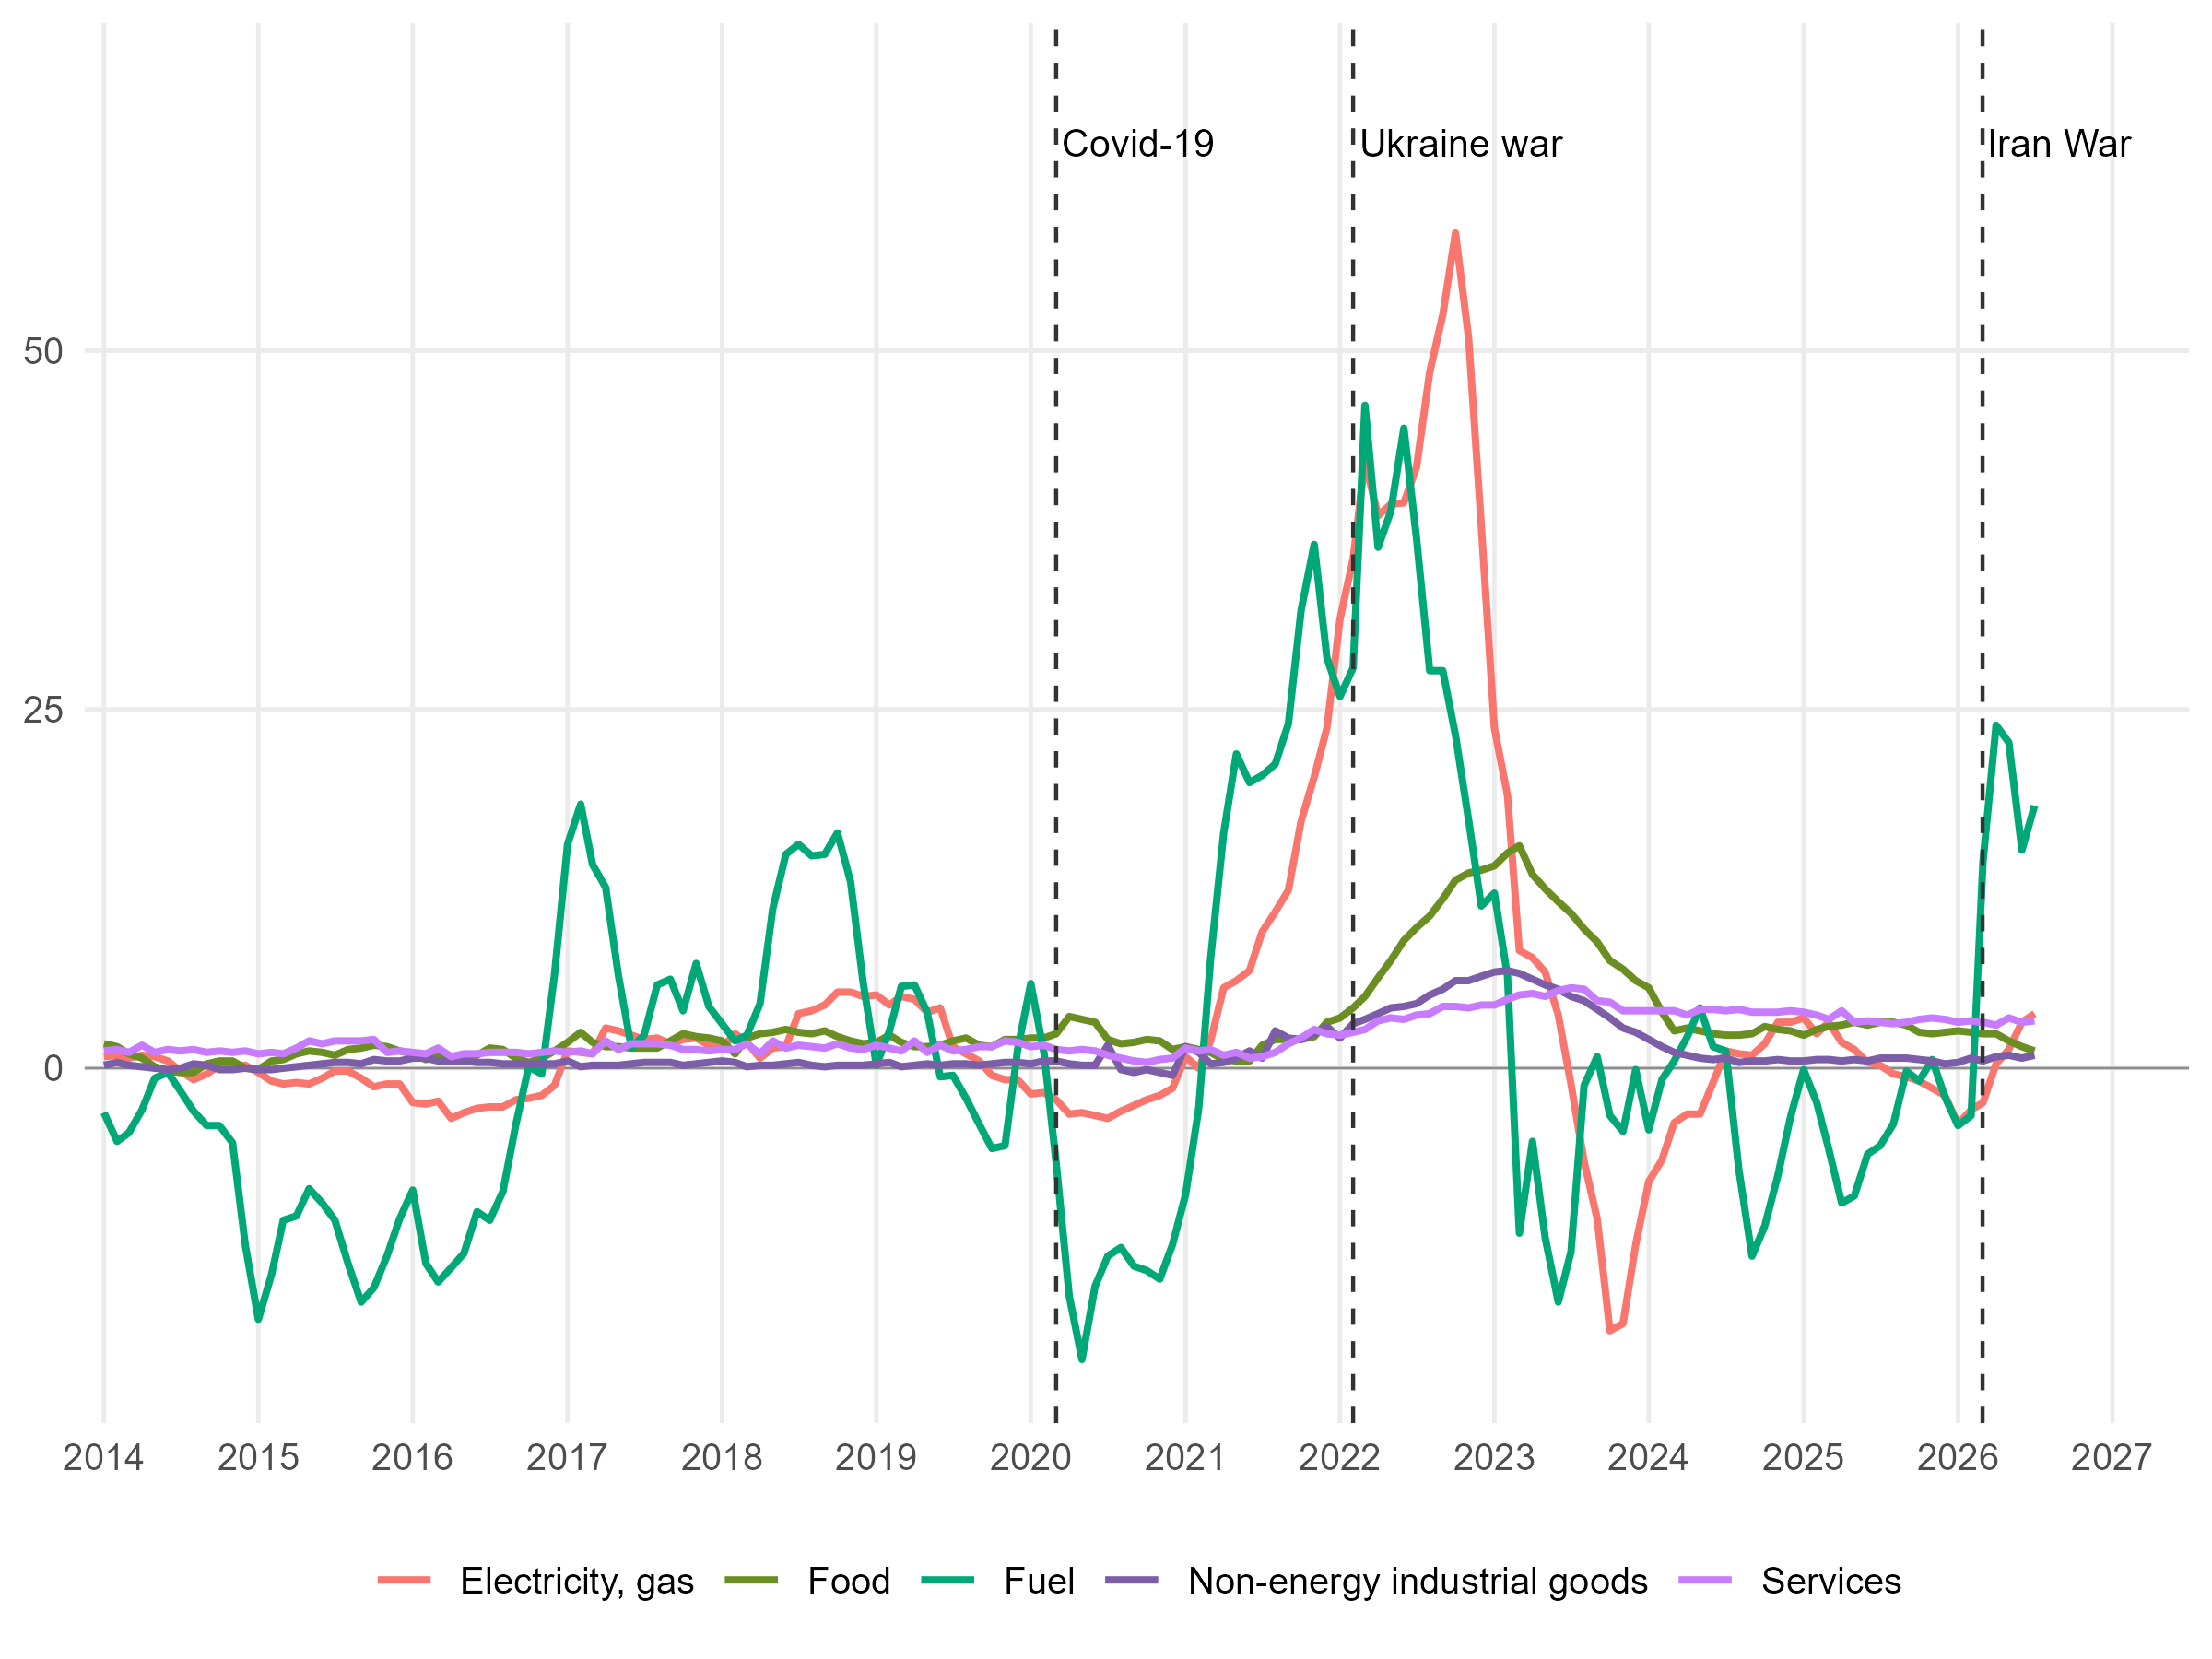
\includegraphics[scale=0.6]{fig/fig_EA_2014_2026_hicp_components.png}
\label{fig:hicp}
\captionsetup{font=footnotesize, format=hang, singlelinecheck=false, justification=justified}
\caption*{%Notes:\\
Sources: Eurostat HICP euro-area aggregate; authors' calculations.}
\end{figure}
%%%%%%%%%%%%%%%%%%%%%%%%%%%%%%%%%%%%%%%%%%%%%%%%%%%%%%%%%%%%%%



\subsection*{Consumption Data and Harmonization Challenges}

The heterogeneity of consumption patterns among households is well-documented, but the accurate
measurement of household-level consumption continues to present significant challenges. Estimating
HICP inflation by household category requires Household Budget Surveys (HBS), which are national
surveys on consumer expenditure.

The Household Budget Surveys cover a large sample (approximately 150,000 households in the euro area).
Households are required to document their expenditures on consumer goods and services over
a designated period, typically two weeks. These surveys capture the values of expenditures across
COICOP categories. HBS data are generally collected every five years.\footnote{See
\citet{accardo2023measuring}, who estimate developments in consumption inequality between survey waves.} The most recent
complete HBS wave generally refers to 2020. Data for this wave were collected between 2018 and 2022
in most EU Member States, with a few country-specific timing exceptions.

National statistical institutes in Italy and Spain also provide higher-frequency HBS data that can be used for country-specific extensions.
Repeated HBS waves available for Spain suggest that, while
behavioral changes over the course of a few years can be significant, point differences
in the weights of the main consumption categories between low- and high-income households remain
relatively stable (see Appendix~\ref{sec:app-additional-hbs-figures}). Changes in
overall consumption patterns may therefore have a limited effect on measured inflation inequality
when consumption shares move in the same direction across income groups.

%%%%%%%%%%%%%%%%%%%%%%%%%%%%%%%%%%%%%%%%%%%%%%%%%%%%%%%%%%%%%%
\begin{figure}[H]
\centering
\caption{Consumption baskets by income quintiles in the euro area (in \% of total expenditures)}
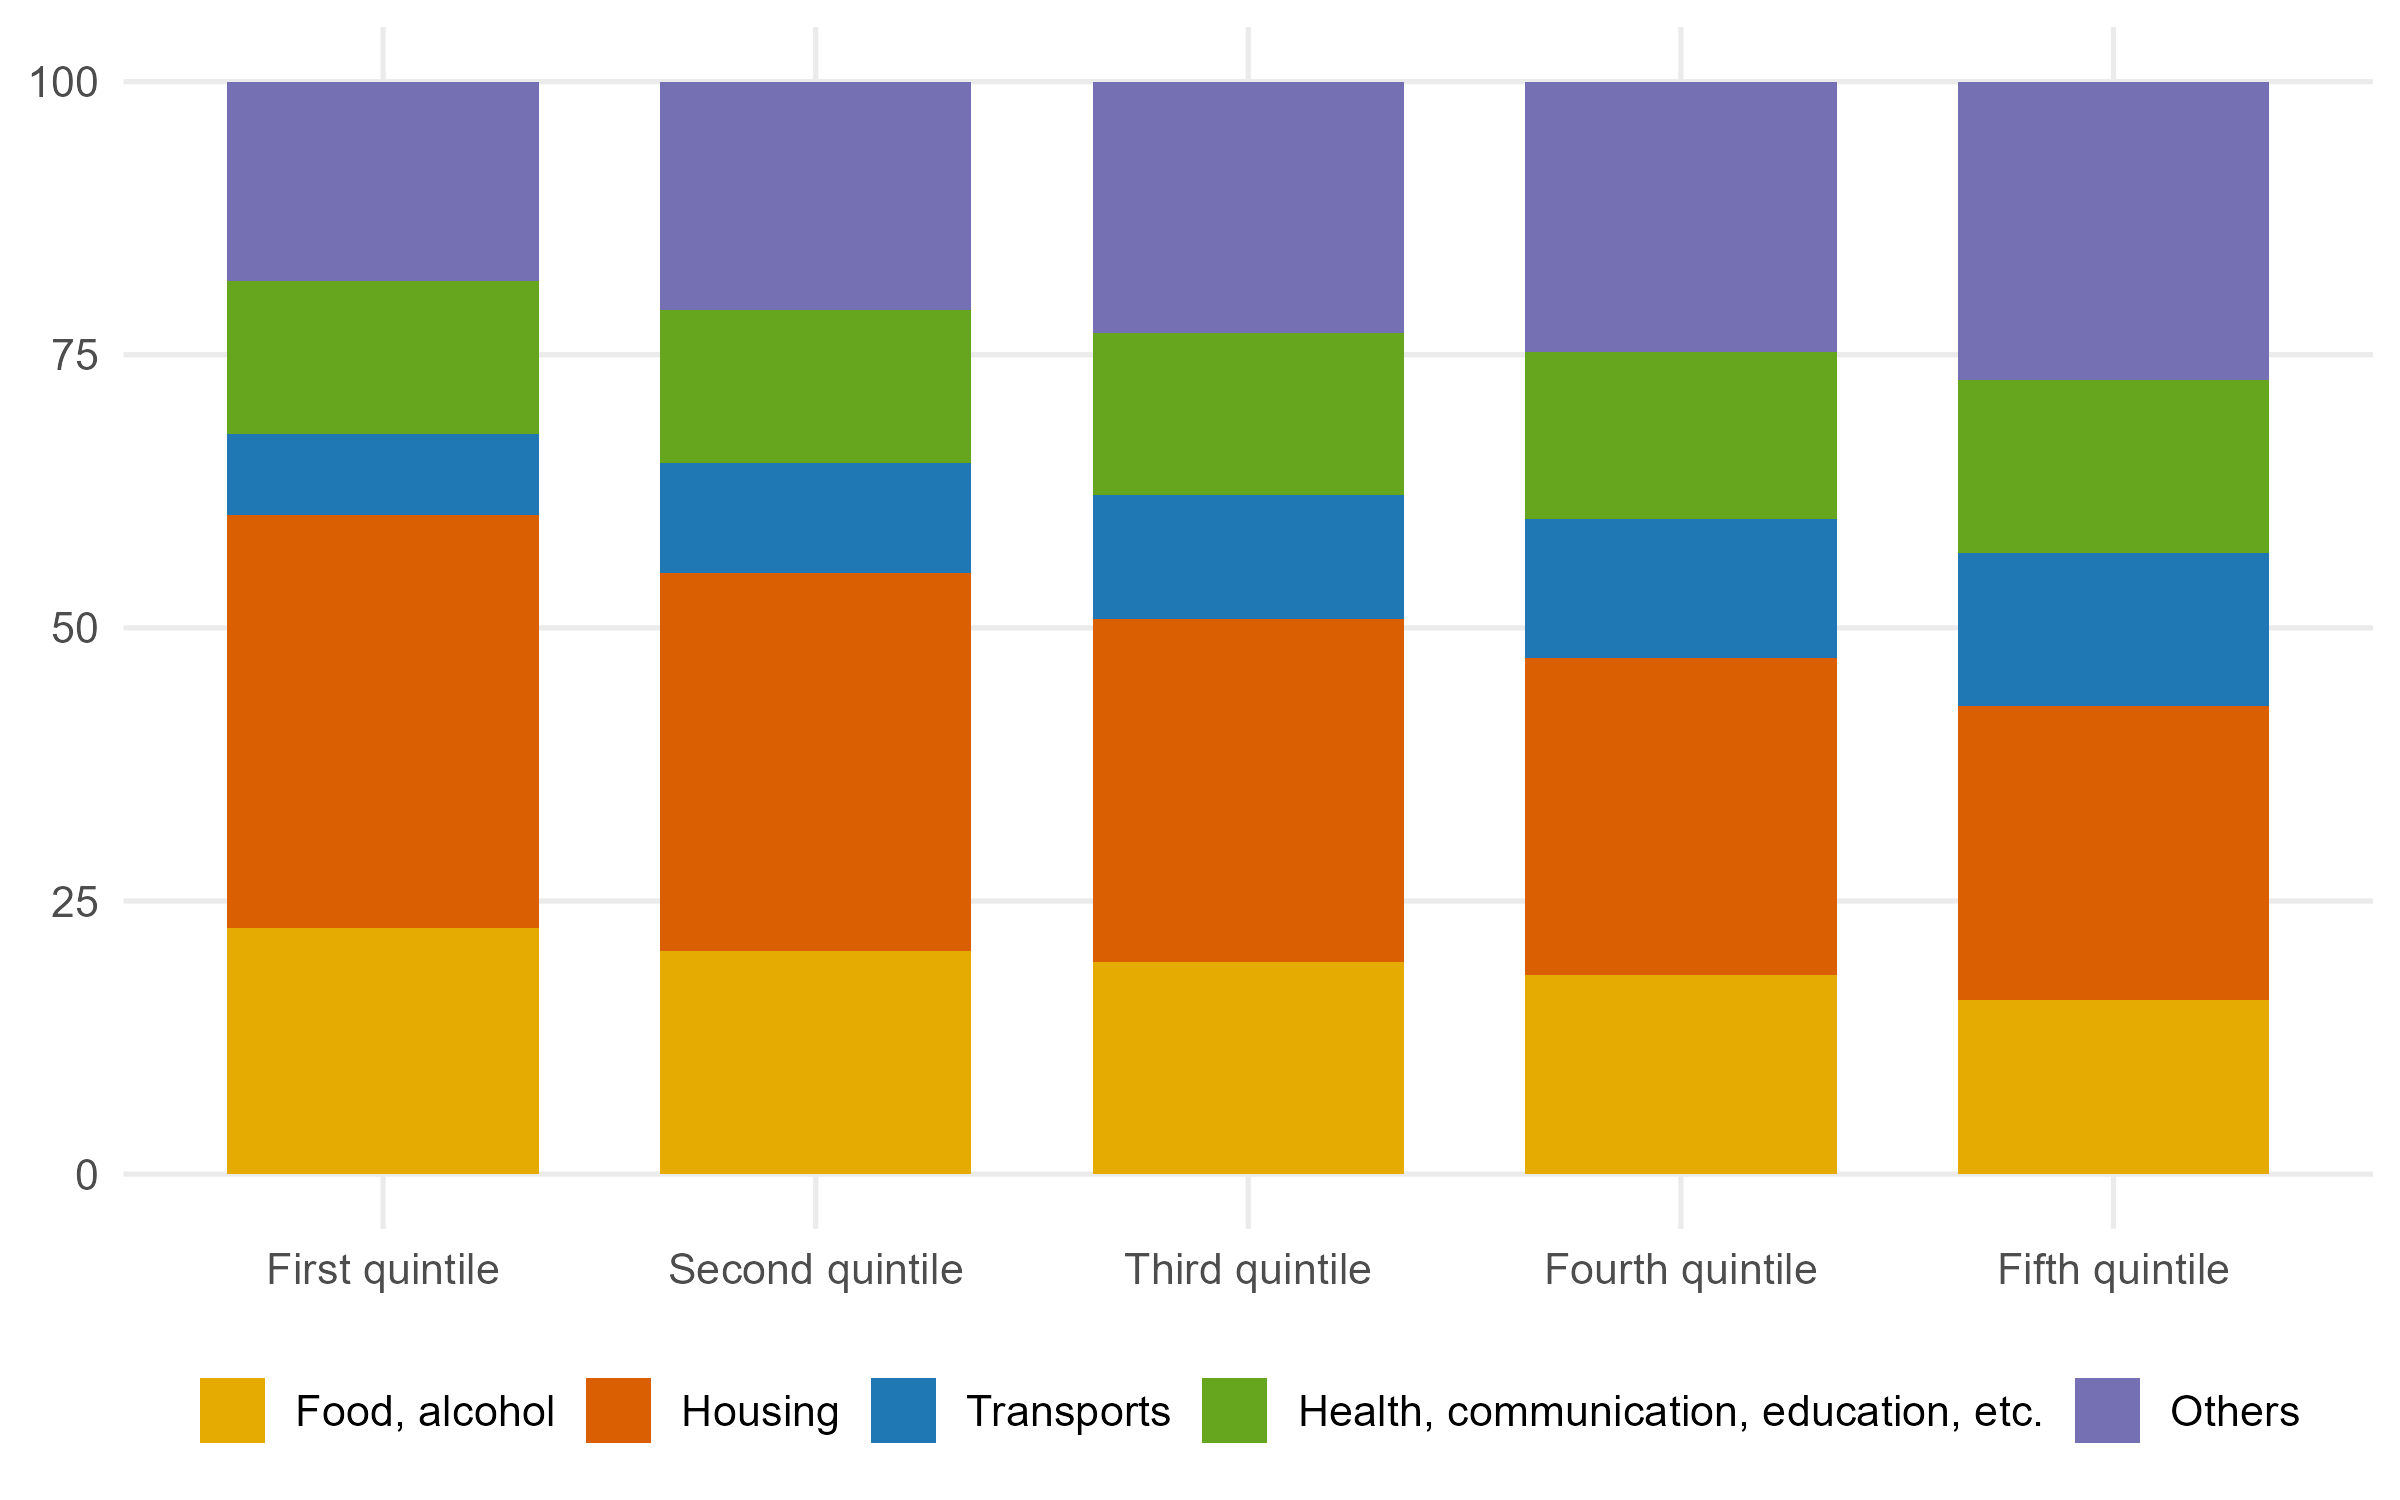
\includegraphics[width=0.86\textwidth,height=0.36\textheight,keepaspectratio]{fig/fig_EA_2020_income_consumption_baskets.png}
\label{fig:hbs}
\captionsetup{font=footnotesize, format=hang, singlelinecheck=false, justification=justified}
\caption*{Notes: Structure of consumption expenditure by income quintile.
The euro-area aggregate combines the 2020 country-level HBS income-quintile
expenditures for all 20 countries and is renormalized to 100 within each
quintile. Italy uses baskets constructed from Istat HBS microdata; see
Appendix~\ref{sec:app-italy-hbs}.\\
Sources: Eurostat HBS, Istat HBS microdata, and authors' calculations.}
\end{figure}
%%%%%%%%%%%%%%%%%%%%%%%%%%%%%%%%%%%%%%%%%%%%%%%%%%%%%%%%%%%%%%


%This infrequent collection may not fully capture short-term fluctuations in consumption patterns, particularly during periods of rapid price changes (e.g. COVID-19), potentially leading to bias in inflation inequality during such periods.\footnote{\cite{accardo2023measuring} developed a methodology to address the issue of low-frequency data in household consumption surveys.} Significant changes in weights between successive waves of HBS can also result in abrupt variations in inflation estimates by category. To address this, a linear interpolation method is proposed to smooth variations.\footnote{To mitigate this issue, two approaches are available in the package: linearly interpolate the HBS weights to smooth out the changes in weights over time, or apply a specific year's HBS weights for all months when calculating inflation rates (or contributions to inflation).}
While HBS expenditure shares are observed only at low frequency, our weighting approach combines
household-specific HBS expenditure structures with monthly HICP inflation rates. As a result,
aggregate consumption patterns can evolve continuously over the business cycle, reflecting changes
in the HICP. However, because cross-household expenditure heterogeneity is assumed to remain constant
between two HBS waves, we use linear interpolation to smooth discrete changes between survey waves.


Figure~\ref{fig:hbs} presents consumption baskets by income quintile. Lower-income households allocate
a larger share of expenditure to essentials such as food and energy, increasing their exposure to
price shocks in these categories. Housing and food account for a substantially larger
share of expenditure among lower-income households. Energy-related expenditure for housing and
private transport is also much higher in rural areas than in cities, reflecting differences in
heating needs and mobility constraints.


HICP and HBS are not directly harmonized. HICP item weights are updated every year and may rely on
national accounts or other national sources, while HBS expenditure structures are observed at lower
frequency. Depending on the level of data available, HICP and HBS are therefore merged at 3-digit
COICOP in each country. In some cases, data published directly by national statistical institutes
can be used instead of relying only on the Eurostat dataset. This approach is particularly valuable
when the nationally published data provide greater granularity, recency, or frequency.\footnote{The
\texttt{inflationinequality} R package allows the use of national data at 4-digit COICOP.}

The HBS contains many household characteristics that can be used to segment inflation exposure. In
this paper, we focus on three dimensions: income, the age of the household reference person, and the
area of residence.\footnote{In recent HBS waves, Eurostat generally requests the Degree of
Urbanisation (DEGURBA) variable, built from a common European methodology based on a 1 km$^2$
population grid. It classifies residence areas into cities (densely populated areas), towns and
suburbs (intermediate density areas), and rural areas (thinly populated areas), using comparable
thresholds across EU countries: urban centers of at least 50,000 inhabitants and 1,500 inhabitants
per km$^2$, urban clusters of at least 5,000 inhabitants and 300 inhabitants per km$^2$, and all
remaining areas.} These variables make it possible to compare inflation experiences not only across
the income distribution, but also across demographic groups and territorial contexts. Although
imputed rent is outside the official HICP coverage, we retain it when constructing group-specific
expenditure profiles; Appendix~\ref{sec:app-weight-normalization} explains this treatment and its
implications for aggregation. Appendix Table~\ref{tab:rent-mapping-robustness} also reports the
sensitivity of the results to alternative rent mappings. For the euro area, the June 2021--June
2023 income-quintile inflation gap is 0.9 point under our baseline mapping of HBS actual
and imputed rents (041+042) to HICP actual rents (041), compared with $-0.5$ point when only HBS
actual rents are mapped to HICP 041 and 1.3 points when rents are excluded altogether. The treatment
of rents therefore matters for the magnitude, and sometimes the sign, of measured inflation
inequality, which supports retaining imputed rents in the group expenditure profiles rather than
redistributing their expenditure share mechanically across non-housing items. This analysis uses all
available waves of the HBS since 1999 and matches them with the closest corresponding HICP year.
Country-specific extensions based on national HBS microdata are described in the appendices when
harmonized Eurostat inputs are incomplete for the required household breakdowns.


%The Consumer Price Index (CPI) and Household Budget Surveys (HBS) are categorized according to the COICOP nomenclature. However, the relationship between the COICOP-CPI and COICOP-HBS classifications is not bijective. To address this, all CPI items are retained while expenditures from the HBS that fall outside the scope of consumption--such as taxes and work-related investment expenditures--are excluded.

% Adjustments are made to the nomenclature for items that lack direct correspondence or are categorized differently. Where feasible, matching is conducted at COICOP digit 4, and at COICOP digit 3 where finer disaggregation is unavailable (e.g., transport services, where modal breakdowns are absent in the HBS), ensuring the inclusion of all CPI products.

%We explain the harmonized methodology applied across all euro area countries, utilizing an R package. The average of inflation measures by categories equals average inflation (cf. Jaravel?). The package allows the use of custom national data where available.
These data constraints motivate the weighting methodology below. A simple use of HBS expenditure
shares would generally not aggregate back to the official HICP, because the HBS all-household basket
does not necessarily coincide with the annually updated HICP item weights. We therefore start from
the official HICP product weights and use HBS only to distribute each product's expenditure across
household groups. The Row and Column Adjustment Scaling (RAS) calibration preserves the relative HBS
expenditure profiles while imposing the row and column margins required by the HICP construction.

\subsection*{Group-Specific Weights}

Let $\omega^{\mathrm{HICP}}_{j,y}$ denote the official annual HICP weight of product category $j$ in weight
year $y$. Let $g$ denote a household group, such as an income quintile, an age group, or a
residence-area group. Let $y'$ denote the HBS wave matched to HICP weight year $y$. Let
$E^{\mathrm{HBS}}_{g,y'}$ and $E^{\mathrm{HBS}}_{\mathrm{all},y'}$ denote total HBS consumption
expenditure by group $g$ and by all households, respectively.

The weights $\omega_{j,g,y}$ are obtained from the RAS calibration. The algorithm preserves the
relative HBS expenditure profiles while making the expenditure-weighted average of group baskets
reproduce the official HICP item weights. Appendix
\ref{sec:app-weight-normalization} describes the RAS algorithm and compares it
with the relative-expenditure normalization.

The calibrated aggregate expenditure matrix $M_{j,g,y}$ is required to satisfy the normalized HICP
item-share margins. Let $s_{g,y}$ denote the share of total household consumption expenditure
accounted for by group $g$ in weight year $y$:
\begin{equation}
s_{g,y}
=
\frac{E^{\mathrm{HBS}}_{g,y'}}{E^{\mathrm{HBS}}_{\mathrm{all},y'}},
\qquad
\sum_g s_{g,y}=1.
\end{equation}
Define the HICP weight normalized over the matched product set as
\[
\bar{\omega}^{\mathrm{HICP}}_{j,y}
=\omega^{\mathrm{HICP}}_{j,y}/
\sum_{k \in \mathcal{J}_y}\omega^{\mathrm{HICP}}_{k,y}.
\]
The RAS calibration imposes:
\begin{equation}
\sum_{j \in \mathcal{J}_y} M_{j,g,y}
=
s_{g,y}
\quad \text{for all } g,
\qquad
\sum_g M_{j,g,y}
=
\bar{\omega}^{\mathrm{HICP}}_{j,y}
\quad \text{for all } j.
\end{equation}

The product margin, $\sum_g M_{j,g,y}=\bar{\omega}^{\mathrm{HICP}}_{j,y}$, ensures that the expenditure-weighted
average of the group-specific weight assigned to each product reproduces the official HICP weight
for that product. The group margin, $\sum_{j \in \mathcal{J}_y} M_{j,g,y}$, fixes the total
expenditure mass of each household group, so that groups can retain different product structures
while aggregating back to the published HICP basket. The final group-specific HICP weight is
obtained by normalizing the calibrated matrix within each group:
\begin{equation}
\omega_{j,g,y}
=
\frac{M_{j,g,y}}{s_{g,y}}
=
\frac{M_{j,g,y}}{\sum_{k \in \mathcal{J}_y}M_{k,g,y}}.
\end{equation}

After aggregation, this calibration closely reproduces the official inflation rate (see
Appendix~\ref{sec:app-weight-normalization}), and validation checks are reported in
Appendix~\ref{sec:app-validation-tests}.

%We use the Household Budget Survey as released by Eurostat once every five years. In contrast, the
%expenditure weights used in the construction of the HICP are updated annually.

The year of the HBS data $y'$ and the HICP weight year $y$ may therefore differ. To align the two sources, each HICP
weight year $y$ is matched with the most recent HBS wave available at or before that year. If no
earlier HBS wave is available, the earliest HBS wave is used.

As a rule, HICP data are available on Eurostat at a level of detail corresponding to the 5-digit
COICOP classification. However, certain product categories lack price data for specific periods. For
instance, early-year price data for medical consultation services ("062") is often unavailable. To
address these gaps, missing price indices are estimated based on the price developments of their
parent product categories. In the case of "062", the price movements of the broader "health
services" category ("06") are used to estimate the missing data.

\subsection*{Group-Level Consumer Price Indices}

Let $p_{j,y,m}$ denote the Laspeyres price index of product category $j$ in month $m$ of year $y$.
Let $p_{j,y,0}$ denote the price reference used for the HICP weight year $y$; in the chained annual
calculation this corresponds to the December price index of the previous year. The aggregation
procedure is as follows: item indices are first unchained within the weight year, aggregated with
annual expenditure weights, and then chained again.\footnote{See Eurostat's \texttt{hicp} R package,
which implements the Eurostat HICP aggregation.} The group-specific within-year price index
therefore combines unchained product indices with the group-specific weights defined above:

\begin{equation}
P_{g,y,m}
=
\sum_{j \in \mathcal{J}_y}
\omega_{j,g,y}
\cdot
\frac{p_{j,y,m}}{p_{j,y,0}}.
\end{equation}

The chained price index for household group $g$, denoted $I_{g,y,m}$, is then obtained by linking
each within-year index to the previous December:

\begin{equation}
I_{g,y,m}
=
I_{g,y-1,12}
\cdot
P_{g,y,m}.
\end{equation}

This notation keeps the two objects distinct: $\omega_{j,g,y}$ is the annual group-specific HICP
weight of product $j$, while $I_{g,y,m}$ is the resulting monthly chained price index for group $g$.


%The HICP data is available on Eurostat at a minimum level of detail corresponding to the 2-digit COICOP classification.

%HICP weights, adjusted each year. HICP weights are used to normalise consumption structures so that aggregation of the indices by category produces the HICP.


%In contrast, essential expenditures, such as housing, food, healthcare, and transportation, constitute almost two-thirds of total consumption for lower-income households, compared to less than half for higher-income households.

\section{Main Results}
\label{sec:main-results}

This section presents our main results. We focus on inflation inequality in the wake of the 2021--23
energy crisis and also document long-run inflation inequality in the euro area.

\subsection{Inflation Inequality in the Euro Area}

%We first describe patterns of inflation inequality over the short run since 2020.

\subsubsection{Short-Run Inflation Inequality}

%Euro area results indicate small or large differences across categories. We also examine product contributions to inflation inequalities.



%In 2022, the contributions of different product categories to the inflation gap (between low and high-income households) tended to cancel each other out (e.g., energy prices vs. services). However, in 2023, rising food prices disproportionately affected low-income households, increasing the inflation gap (Figure 3).

Figure~\ref{fig:ea20_short_run_income} shows that the post-COVID inflation surge translated
into moderate income-based inflation inequality in the euro area. Inflation
rates for the first and fifth income quintiles remained close throughout the 2021--2023
period. Energy and food shocks raised headline inflation sharply, but their effects on the relative
inflation exposure of low- and high-income households largely offset once national consumption
structures and country-level price dynamics are combined across all 20 countries.

This pattern is broadly consistent with recent evidence from \citet{bobasu2023impact} and
\citet{claeys2022inflation}, although small differences remain because of our weighting scheme and
treatment of imputed rents.

%%%%%%%%%%%%%%%%%%%%%%%%%%%%%%%%%%%%%%%%%%%%%%%%%%%%%%%%%%%%%%
\begin{figure}[H]
\centering
\caption{Short-run inflation inequality in the euro area, by income quintile (year on year, in \%)}
\label{fig:ea20_short_run_income}
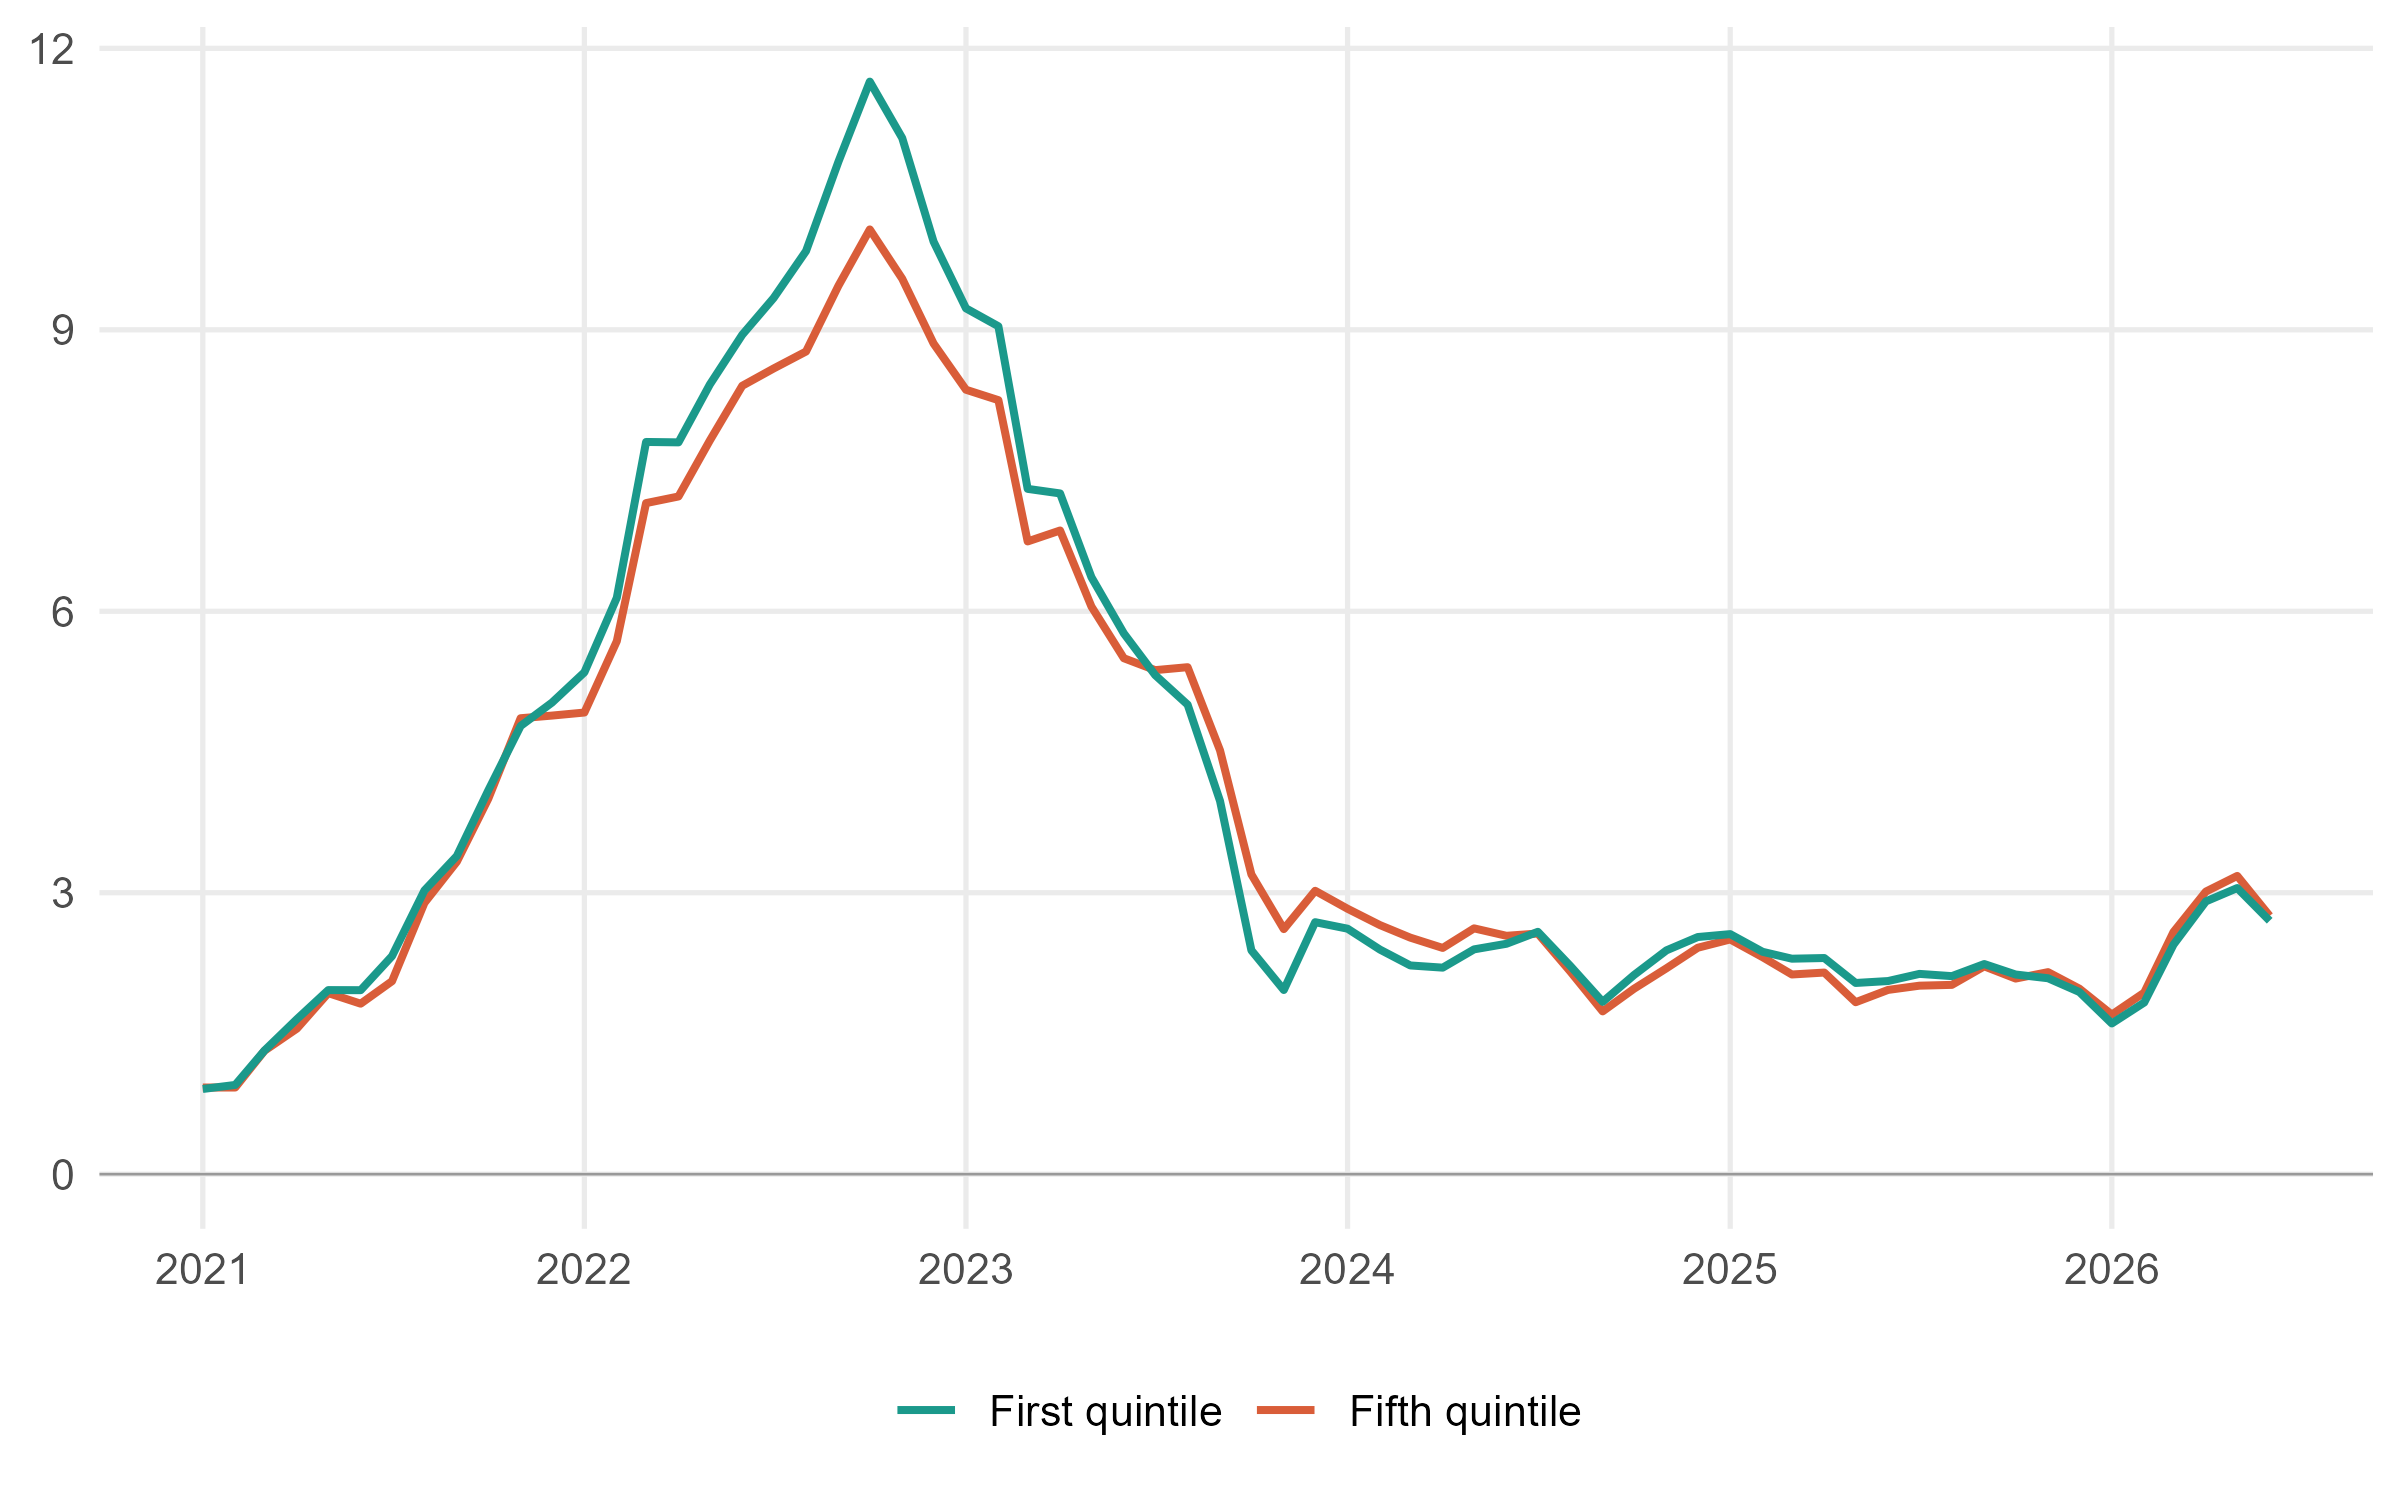
\includegraphics[scale=0.6]{fig/fig_EA20_2020_2026_income_inflation_Q1_Q5.png}
\vspace{6pt}
\captionsetup{font=footnotesize, format=hang, singlelinecheck=false, justification=justified}
\caption*{Notes: This figure reports year-on-year inflation rates for the first and fifth income quintiles in the euro area from January 2020 to July 2026. The country series are aggregated using annual HICP country weights.\\
Sources: Eurostat HICP, HBS, authors' calculations}
\end{figure}
%%%%%%%%%%%%%%%%%%%%%%%%%%%%%%%%%%%%%%%%%%%%%%%%%%%%%%%%%%%%%%
\newpage


\subsubsection{Inflation Inequality by Age and Residence Area}

%Papers on inflation inequality focus on inequality according to household income brackets. However, in the case of most countries, it was inflation differentials between age groups or residence areas that were much more pronounced during the 2021-2023 period.

Figure~\ref{fig:age_rural} presents inflation rates by household category in the euro area,
segmented by age and residence area. To ensure comparability with the 0.9-point cumulative Q1--Q5
gap, we compute all three gaps from chained price-index changes between June 2021 and June 2023,
using indices based in 2020 and the same annual HICP country weights. Cumulative inflation was 15.2
percent for households aged 60 or over and 13.9 percent for households under 30, yielding an age gap
of 1.3 points. It was 15.3 percent in rural areas and 14.3 percent in cities, yielding a rural--city
gap of 1.0 point. The monthly annual inflation rates in the figure show that both gradients varied
over time and temporarily narrowed or reversed as energy inflation receded.

The residence-area differentials reflect differences in the structure of
energy demand. Rural households tend to spend a larger share of their budget on transport fuels and
home energy, partly because commuting distances are longer and the set of available transport
substitutes is more limited. This raises their exposure when energy prices accelerate, but also makes
their measured inflation fall faster when those price pressures unwind.

%%%%%%%%%%%%%%%%%%%%%%%%%%%%%%%%%%%%%%%%%%%%%%%%%%%%%%%%%%%%%%
\begin{figure}[H]
\centering
\caption{Inflation by household categories in the euro area (year on year, in \%)}
\label{fig:age_rural}
\begin{subfigure}{0.48\textwidth}
  \centering
  \caption{By age}
  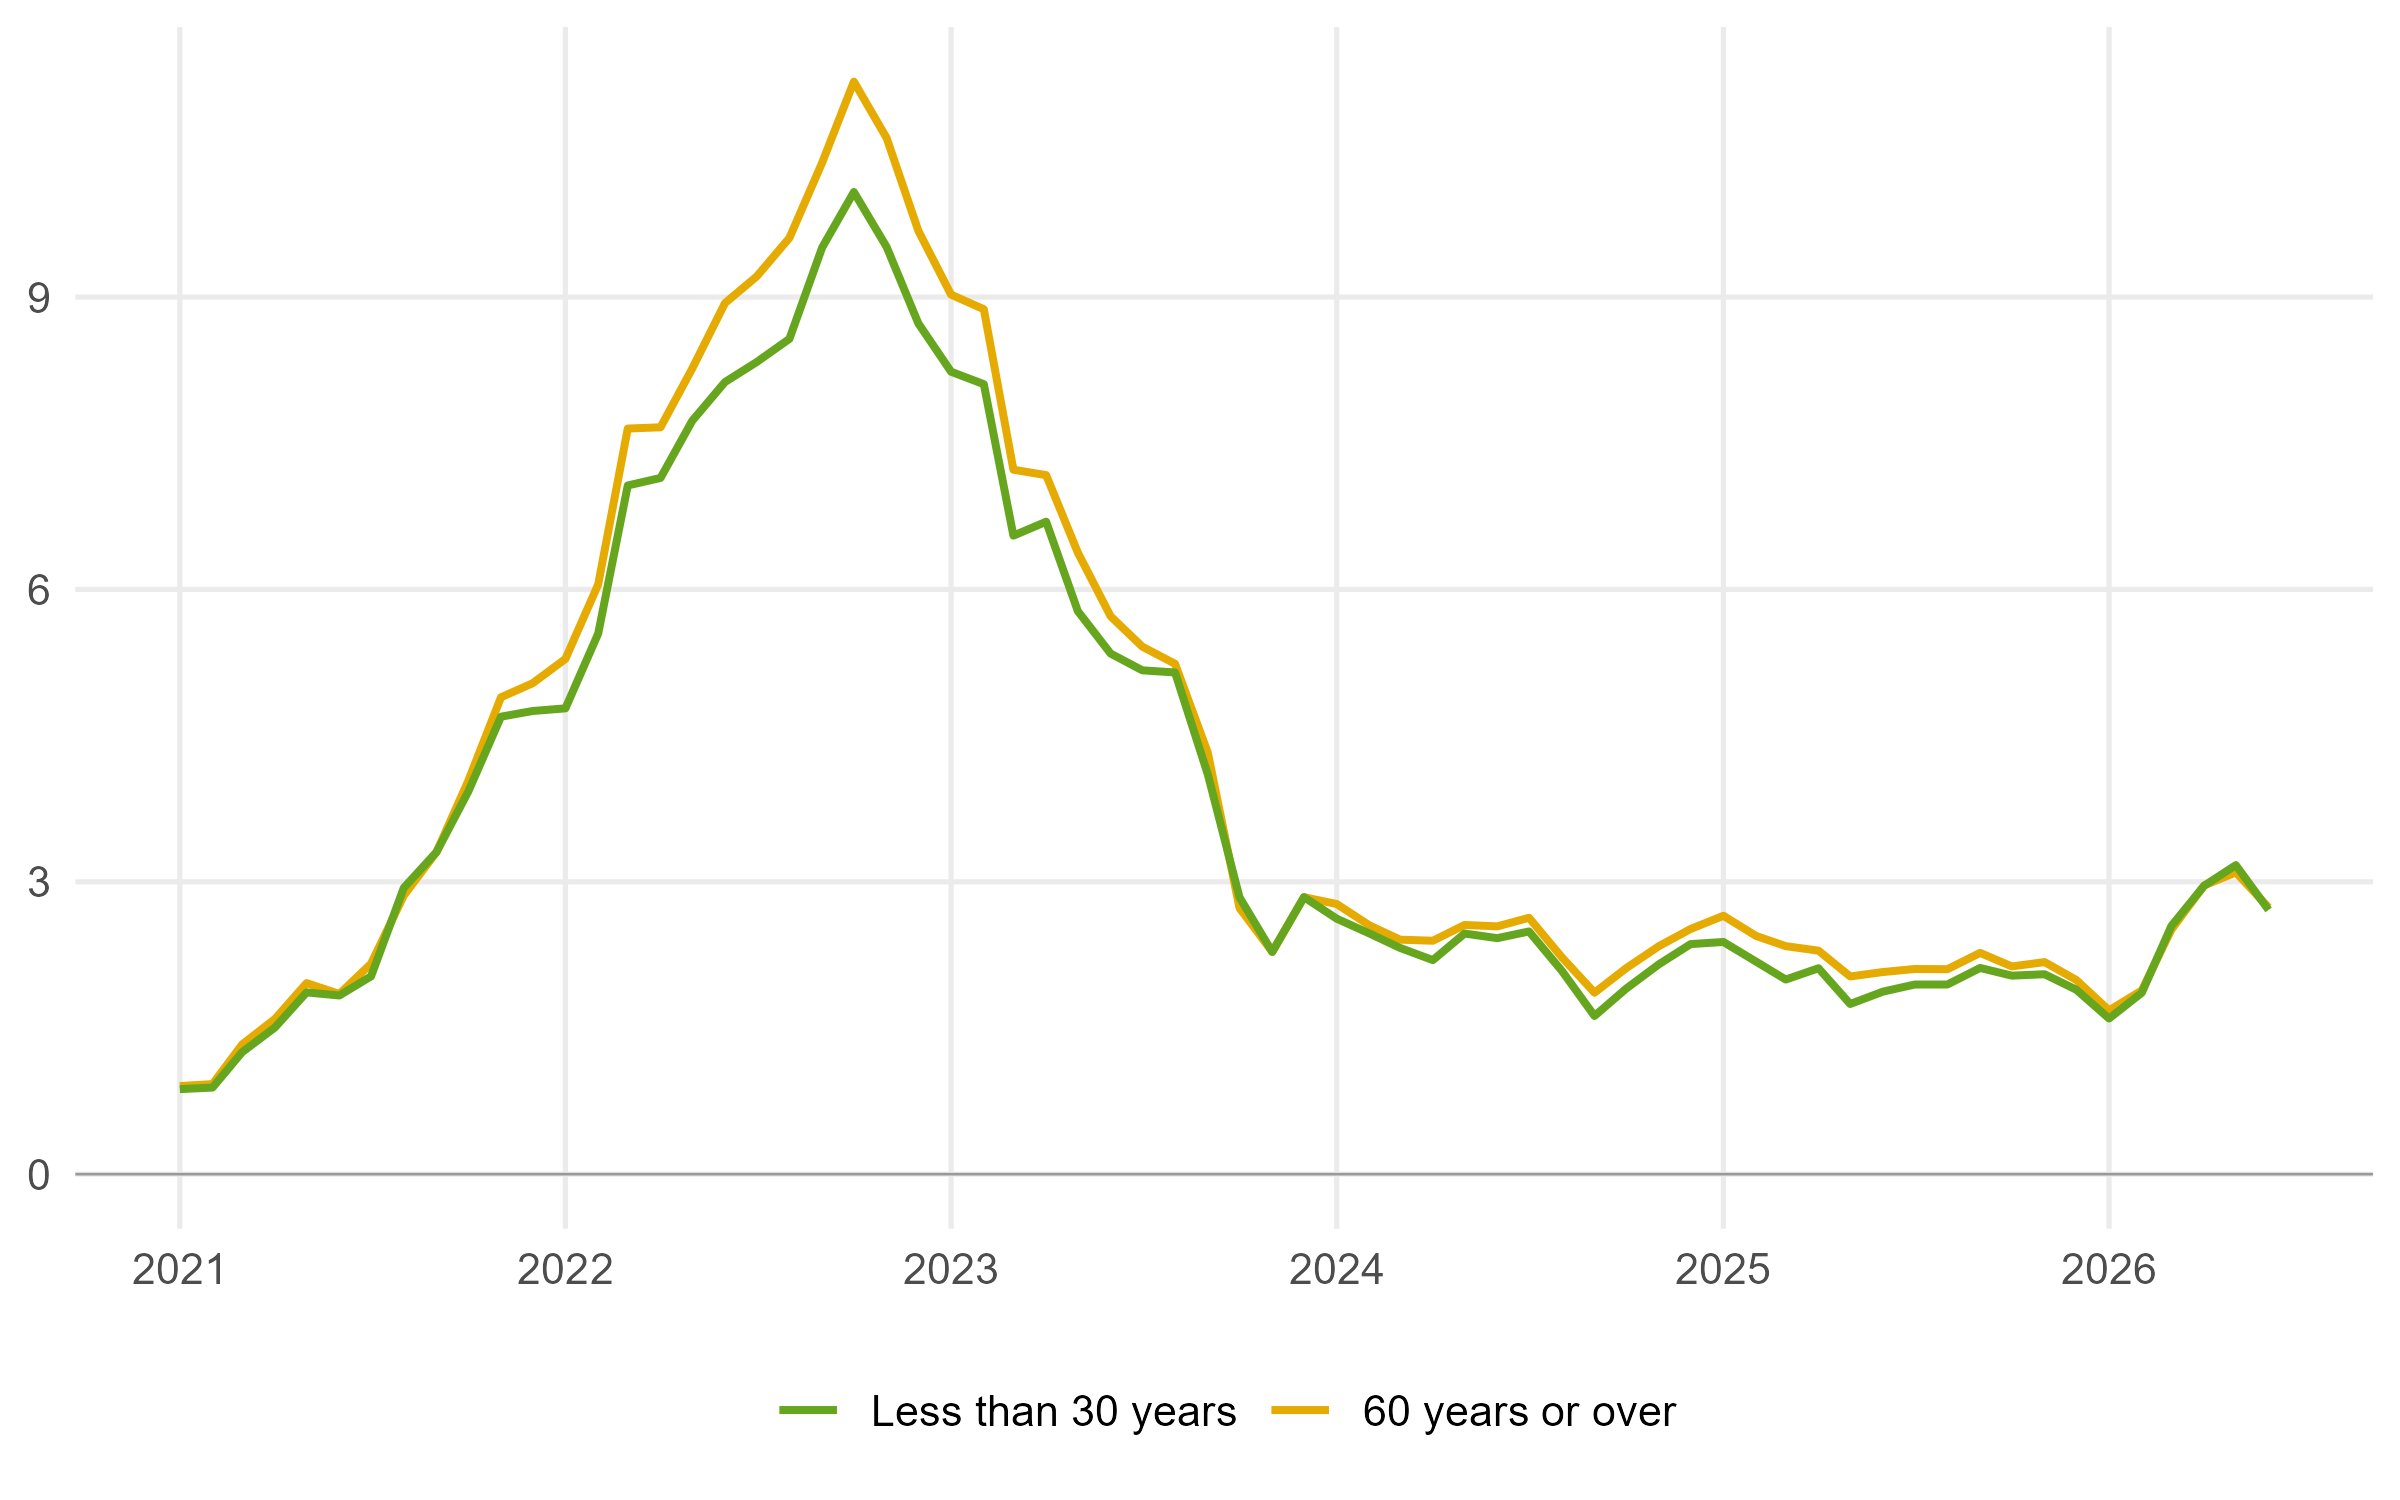
\includegraphics[width=\linewidth,height=6cm]{fig/fig_EA20_2020_2026_age_inflation_under30_60plus.png}
\end{subfigure}
\hfill
\begin{subfigure}{0.48\textwidth}
  \centering
  \caption{By residence area}
  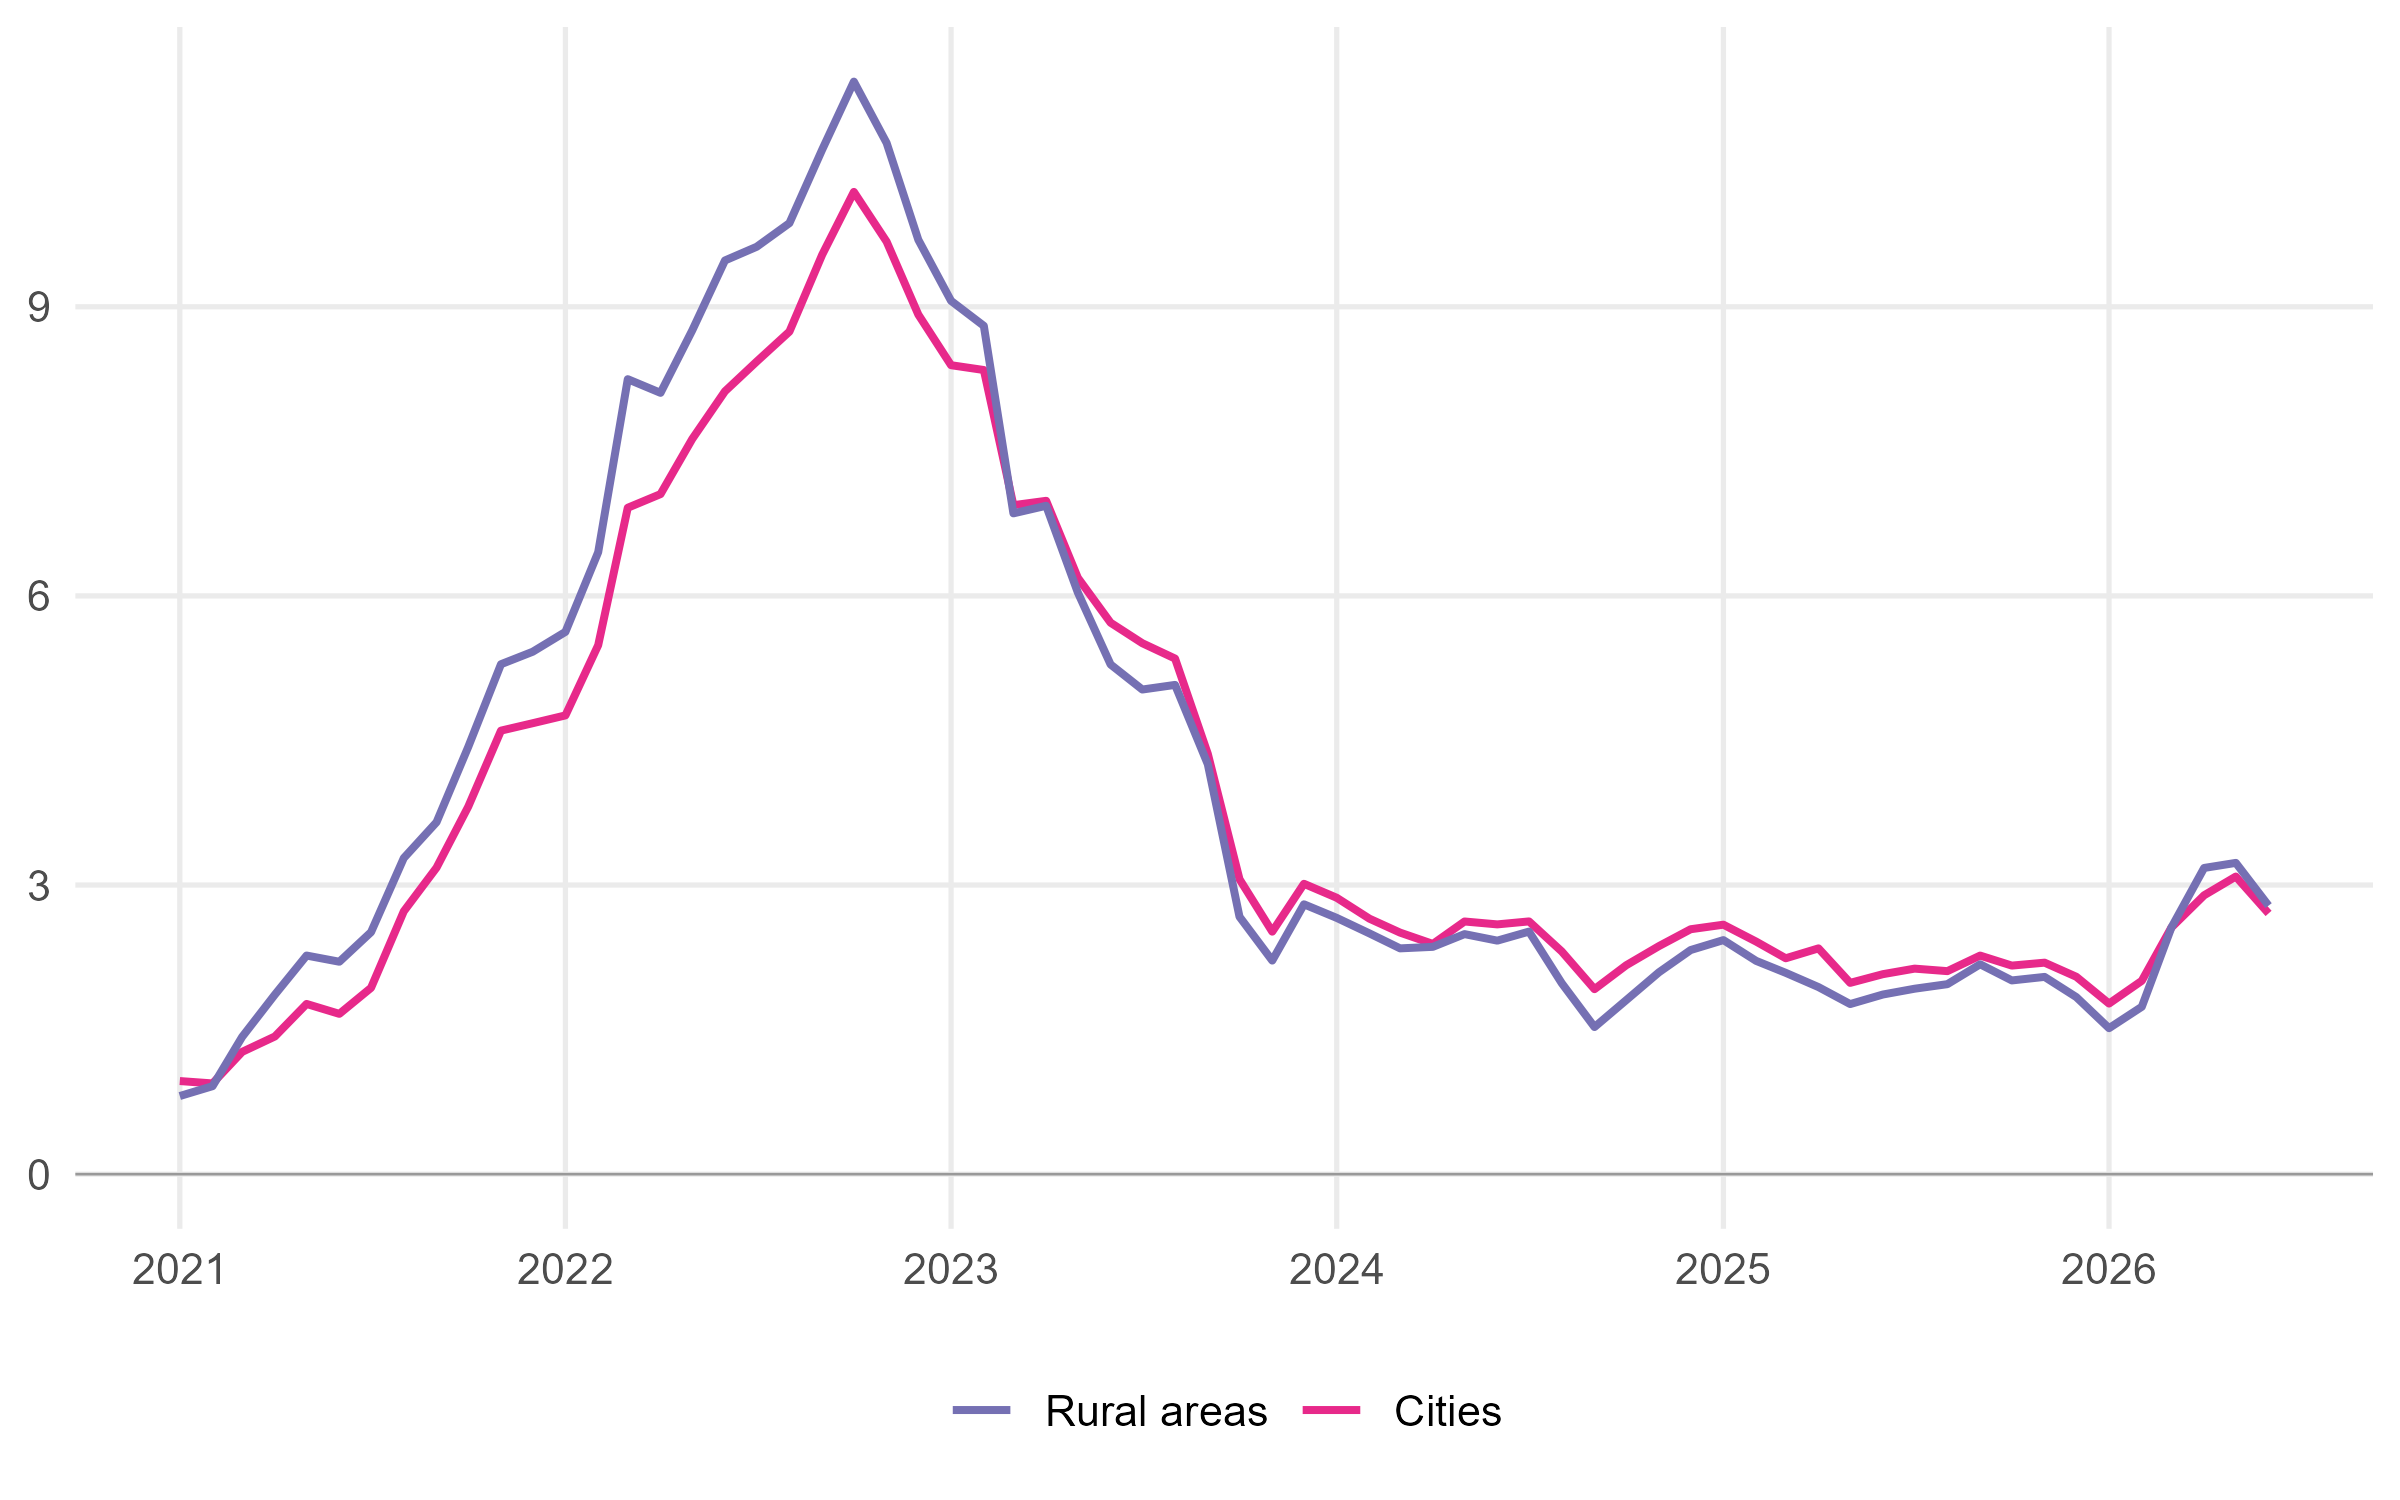
\includegraphics[width=\linewidth,height=6cm]{fig/fig_EA20_2020_2026_urban_inflation_rural_cities.png}
\end{subfigure}
%\label{fig:5}
\vspace{10pt}
\captionsetup{font=footnotesize, format=hang, singlelinecheck=false, justification=justified}
\caption*{Notes: This figure reports year-on-year inflation rates in the euro area by
age (panel a) and residence area (panel b), January 2020 to July 2026. The cumulative gaps discussed
in the text use the same endpoints as the income gap, June 2021 and June 2023, and are calculated as
$100(P_{g,2023\text{-}06}/P_{g,2021\text{-}06}-1)$ for each group before taking the difference.
For age, cumulative inflation is 15.17 percent for households aged 60 or over and 13.90 percent for
households under 30; the 60-or-over minus under-30 gap is therefore 1.27 points, rounded to 1.3. For
residence, cumulative inflation is 15.27 percent in rural areas and 14.31 percent in cities; the
rural--city gap is therefore 0.96 point, rounded to 1.0. All series use chained indices based in
2020 and annual HICP country weights.\\
Sources: Eurostat HICP, HBS, authors' calculations}
\end{figure}
%%%%%%%%%%%%%%%%%%%%%%%%%%%%%%%%%%%%%%%%%%%%%%%%%%%%%%%%%%%%%%
\newpage


\subsubsection{Long-Run Inflation Inequality}

Figure~\ref{fig:ea20_long_run_income} shows a modest but persistent divergence between the first- and
fifth-quintile price indices after 2008. The post-COVID episode produced the largest visible widening
in the series since 2000.

% This suggests that, once country aggregation is taken into account, the
%recent inflation surge was primarily a rather than a strong source of
% inflation inequality for the euro area as a whole.

%%%%%%%%%%%%%%%%%%%%%%%%%%%%%%%%%%%%%%%%%%%%%%%%%%%%%%%%%%%%%%
\begin{figure}[H]
\centering
\caption{Long-run inflation inequality in the euro area, by income quintile (index, 2000 = 100)}
\label{fig:ea20_long_run_income}
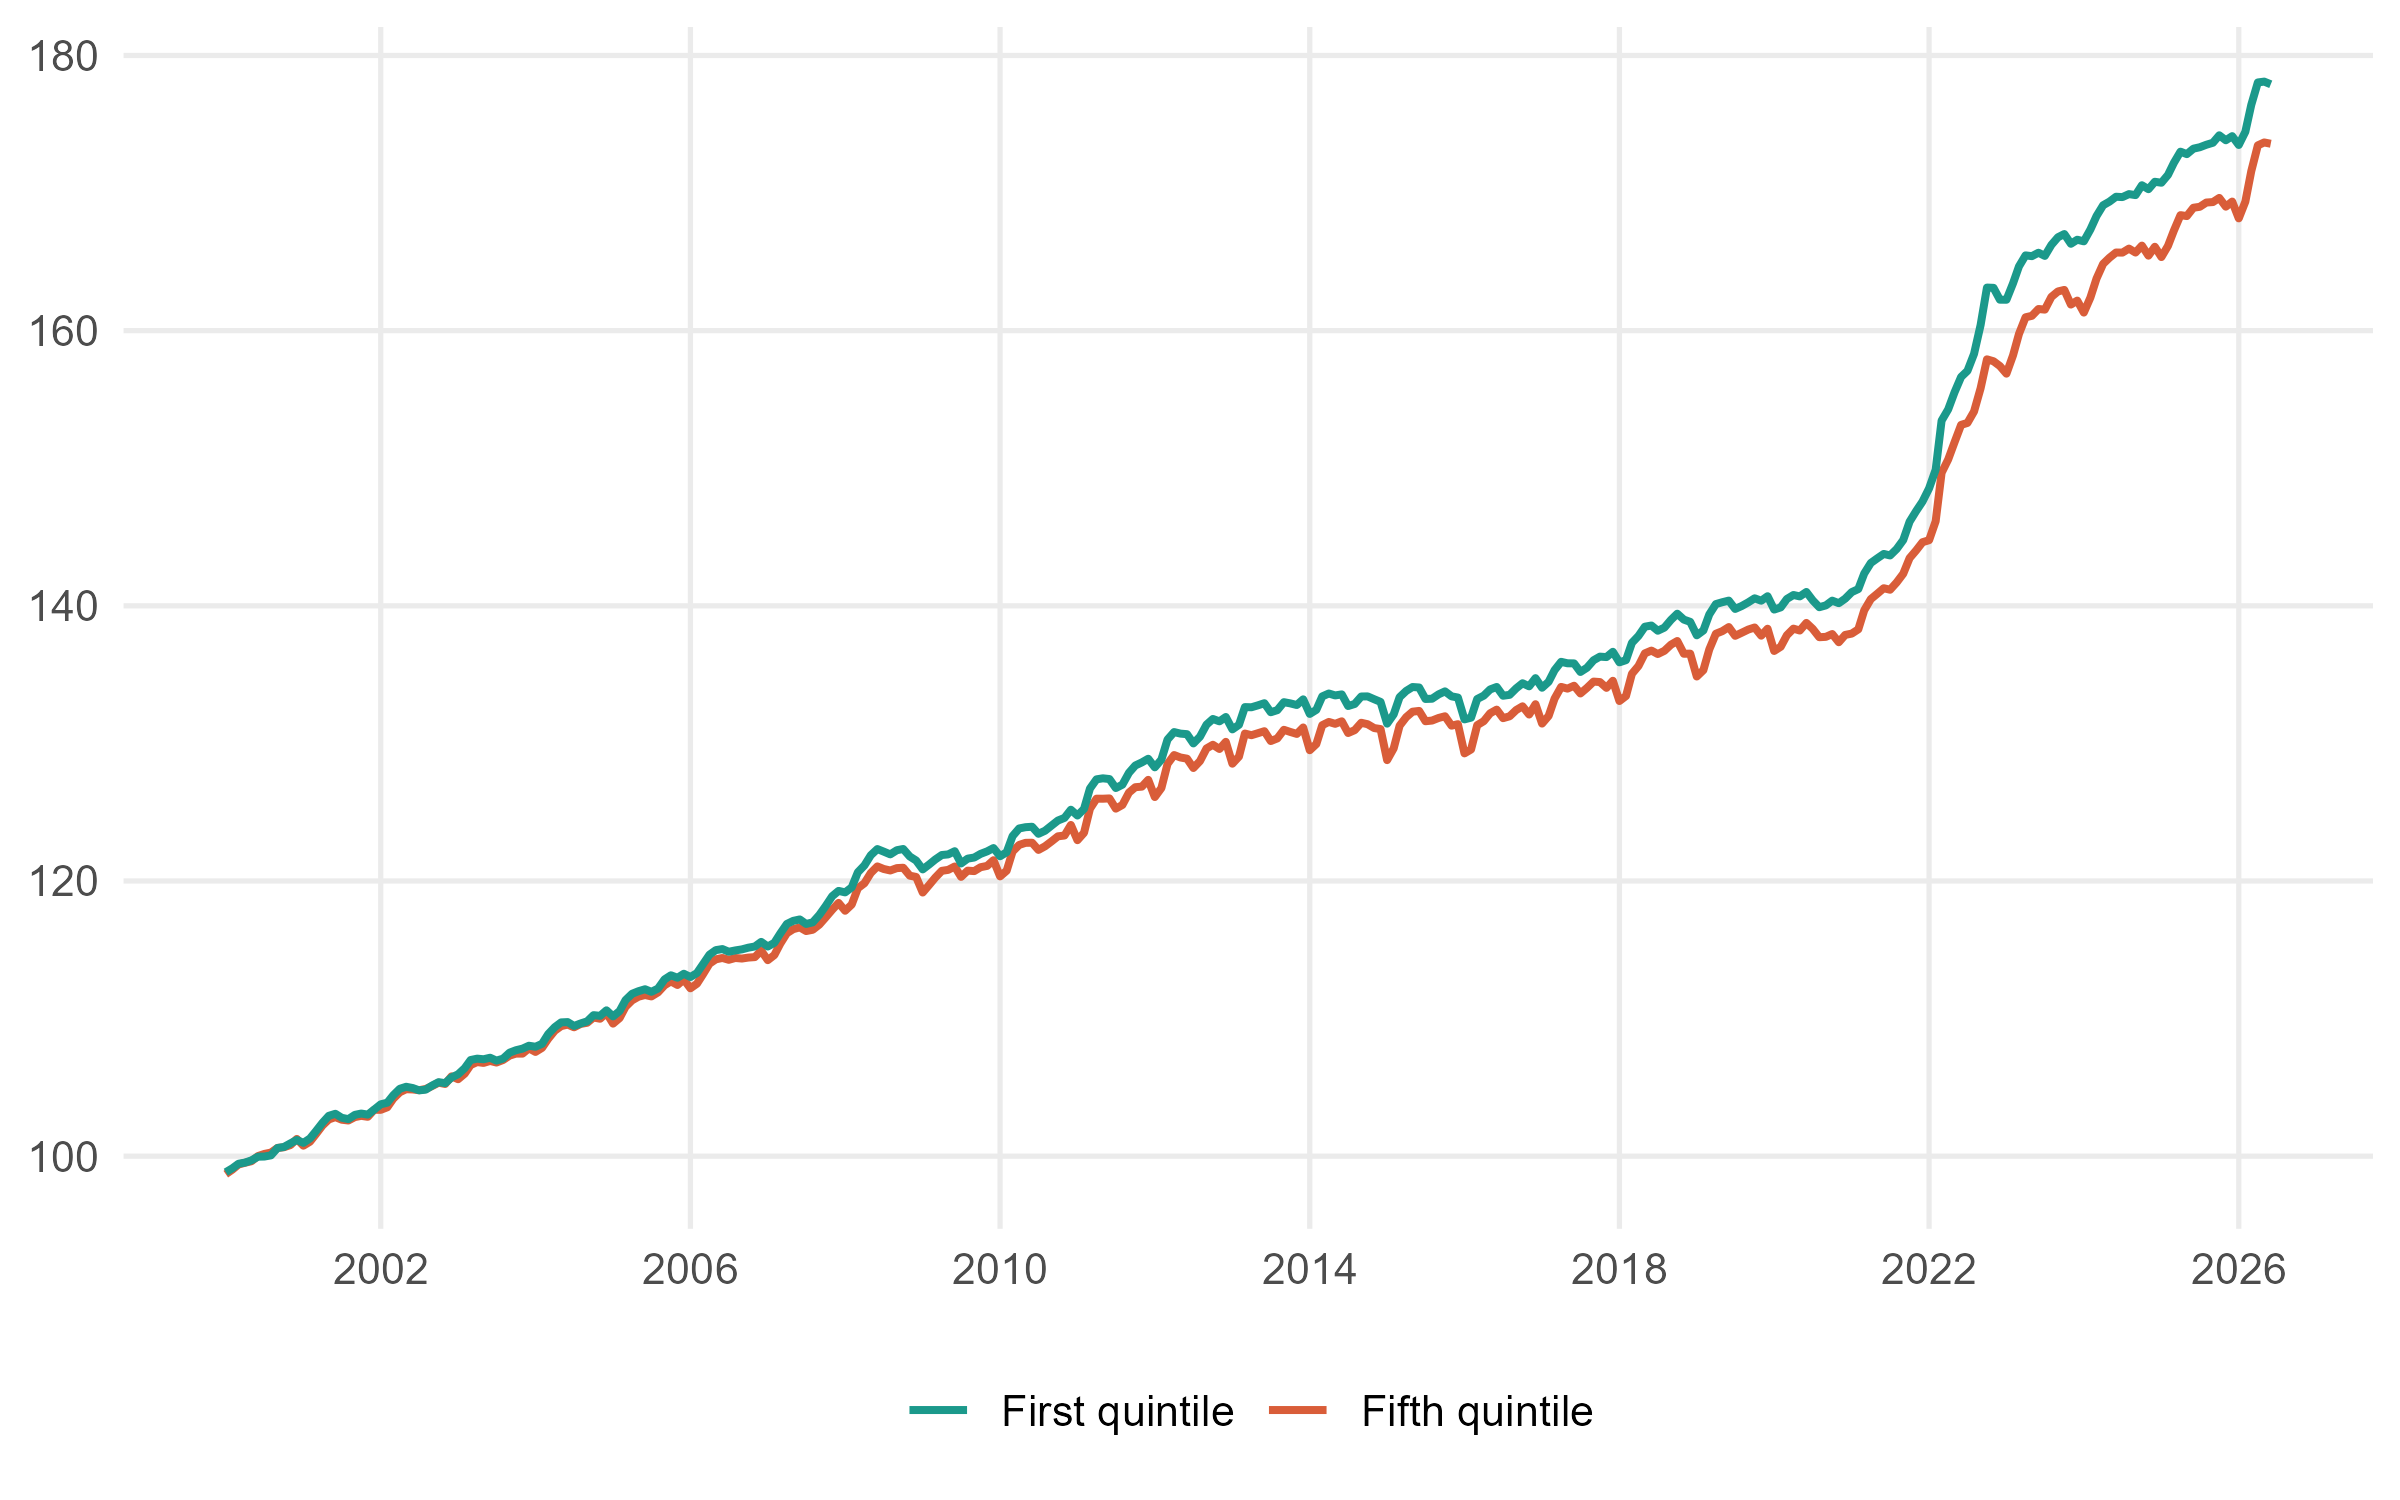
\includegraphics[width=0.76\textwidth,height=0.27\textheight,keepaspectratio]{fig/fig_EA20_2000_2026_income_price_index_Q1_Q5_base2000.png}
\vspace{3pt}
\captionsetup{font=footnotesize, format=hang, singlelinecheck=false, justification=justified}
\caption*{Notes: This figure shows monthly price indices for the first and fifth income quintiles in the euro area, January 2000 to July 2026. Indices are rebased to 2000 = 100.\\
Sources: Eurostat HICP, HBS, authors' calculations}
\end{figure}
%%%%%%%%%%%%%%%%%%%%%%%%%%%%%%%%%%%%%%%%%%%%%%%%%%%%%%%%%%%%%%

This pattern contrasts with the larger long-run gaps documented for the United States in
\cite{jaravel2024distributional}. Several methodological differences may account for the contrasting results. First, the
euro-area indices reported here aggregate national indices and therefore average across countries
whose price dynamics and fiscal responses can offset one another. Second, the euro-area calculation
uses harmonized 3-digit COICOP categories, whereas the U.S. evidence exploits much finer product-level
data. Aggregation within broad categories can conceal persistent differences in the prices paid by
different income groups, which are captured in the U.S. data.


%The resulting euro-area long-run gap should
%therefore be interpreted as a between-category measure and may understate within-category inflation
%inequality.

%\cite{jaravel2021inflation} identifies two key factors explain the different consumption patterns of households. First, technological progress tend to disproportionately benefit higher-income households. Second, globalization has not provided significant compensatory benefits to lower-income households. Instead, its advantages have largely bypassed these groups, exacerbating existing disparities rather than mitigating.

\subsection{Heterogeneous Effects of the 2022--23 Energy Shock Across Countries}

%We observe heterogeneity in inflation inequalities across the euro area. Is there a link between inflation inequalities and inflation levels?

%\subsection*{Four different Patterns of Inflation Inequality}

The 2021--23 inflation episode was marked by a large energy-price shock, especially in natural gas markets,
following Russia's invasion of Ukraine. Although this shock was common to the euro area, its
distributional effects differed across countries because energy mixes, import dependence, household
consumption patterns, and fiscal responses were not uniform.

Table~\ref{tab:country-heterogeneity-cumulative-gap} documents this cross-country heterogeneity by
reporting the cumulative June 2021--June 2023 inflation gap between the first and fifth income quintiles. The
Baltic countries and Ireland display large positive Quintile 1--Quintile 5 gaps, while several large
economies show more compressed gaps.

The interaction between country-specific price dynamics, exposures, and fiscal policies and
group-specific expenditure shares explains these differences. A price increase in a product category generates inflation inequality only to
the extent that the affected category has different expenditure weights across household groups.
Hence, similar income-quintile consumption profiles can still produce different inflation gaps when
national energy prices, food prices, or fiscal cushioning measures evolve differently. Conversely,
large aggregate shocks may generate limited inequality when price increases fall on categories with
similar weights across quintiles or when policy measures dampen prices in essential energy
components.


%%%%%%%%%%%%%%%%%%%%%%%%%%%%%%%%%%%%%%%%%%%%%%%%%%%%%%%%%%%%%%
\begin{table}[H]
\small
\setlength{\tabcolsep}{5pt}
\renewcommand{\arraystretch}{0.95}

\caption{\label{tab:country-heterogeneity-cumulative-gap}Cumulative inflation gap between the first and fifth income quintiles, January 2021--December 2023}
\centering
\begin{tabular}[t]{lllllll}
\toprule
\multicolumn{3}{c}{} & \multicolumn{4}{c}{Inflation gap}\\
\cmidrule(lr){4-7}
Country & \shortstack{Weight\\(2022, \%)} & \shortstack{Cumulative\\inflation} & 2021--2023 & 2021 & 2022 & 2023\\
\midrule
Germany & 28.1 & 18.6 & 0.5 & -0.4 & 0.9 & 0.4\\
France & 20.4 & 14.6 & 0.7 & 0.3 & 0.1 & 0.1\\
Italy & 16.3 & 18.7 & 1.3 & 0.1 & 1.5 & 0.4\\
Spain & 11.0 & 16.5 & -0.2 & 0.8 & 0.9 & -0.7\\
Netherlands & 5.4 & 20.1 & 0.6 & -0.3 & 1.8 & -0.9\\
\addlinespace
Belgium & 4.0 & 19.1 & -0.3 & 1.2 & 1.9 & -2.3\\
Austria & 3.3 & 22.0 & -0.4 & -0.5 & -0.2 & 0.5\\
Portugal & 2.2 & 15.4 & -0.4 & 0.7 & 0.1 & -0.9\\
Greece & 2.2 & 17.9 & 1.4 & 0.3 & 1.2 & -0.5\\
Finland & 1.9 & 13.2 & -1.0 & -0.2 & -1.1 & 0.2\\
\addlinespace
Ireland & 1.5 & 17.8 & 4.2 & 0.4 & 2.8 & 1.1\\
Slovakia & 0.8 & 28.4 & 2.1 & -0.9 & 1.1 & 1.3\\
Croatia & 0.7 & 24.7 & -0.4 & 0.0 & 0.3 & -0.3\\
Lithuania & 0.6 & 34.3 & 3.6 & 0.2 & 3.3 & 0.4\\
Slovenia & 0.4 & 21.2 & 1.3 & 0.1 & 0.5 & 1.4\\
\addlinespace
Luxembourg & 0.3 & 14.5 & 0.3 & 0.1 & 0.2 & -0.1\\
Latvia & 0.3 & 30.8 & 5.9 & -0.2 & 4.6 & 2.4\\
Estonia & 0.2 & 36.5 & 6.8 & 0.5 & 4.3 & 1.5\\
Cyprus & 0.2 & 15.9 & 0.3 & 0.0 & 0.7 & 0.2\\
Malta & 0.1 & 15.7 & 1.7 & -0.4 & 0.2 & 1.2\\
\addlinespace
\midrule
\textbf{Euro area} & \textbf{100.0} & \textbf{17.8} & \textbf{0.6} & \textbf{0.1} & \textbf{0.9} & \textbf{0.0}\\
\bottomrule
\end{tabular}
\vspace{-0.4em}
\begin{flushleft}
\footnotesize{Notes. Cumulative changes compare January 2021 with December 2023; annual rates compare annual-average indices. The gap is Q1 minus Q5. Weights are 2022 EA20 HICP shares. National product indices are first aggregated within each country; national monthly movements are then aggregated to EA20 using annual country weights. The same observed product-country pipeline feeds Table~2. Entries are percentage points. Sources: Eurostat, authors' calculations.}
\end{flushleft}
\end{table}

%%%%%%%%%%%%%%%%%%%%%%%%%%%%%%%%%%%%%%%%%%%%%%%%%%%%%%%%%%%%%%

Housing energy and food raised the Quintile 1--Quintile 5 gap by 2.2 points between June 2021 and
June 2023, but transport offset more than half of that increase
(Table~\ref{tab:ea20-income-gap-product-contributions}).

%%%%%%%%%%%%%%%%%%%%%%%%%%%%%%%%%%%%%%%%%%%%%%%%%%%%%%%%%%%%%%
\begin{table}[H]
\small
\setlength{\tabcolsep}{4.2pt}
\renewcommand{\arraystretch}{0.95}

\caption{\label{tab:ea20-income-gap-product-contributions}Product-group contributions to euro-area cumulative income inflation gaps, January 2021--December 2023}
\centering
\resizebox{\textwidth}{!}{%
\begin{tabular}{lrrrrr}
\toprule
Product group & Product weight & Cumulative inflation & Q1 contribution & Q5 contribution & Inflation gap\\
\midrule
Food and non-alcoholic beverages & 16.6 & 4.4 & 5.2 & 3.8 & 1.4\\
Alcoholic beverage, tobacco and narcotics & 4.3 & 0.6 & 0.9 & 0.4 & 0.4\\
Clothing and footwear & 5.2 & 1.0 & 0.8 & 1.1 & -0.3\\
Housing (rentals and repairs) & 12.2 & 1.7 & 1.4 & 1.8 & -0.4\\
Water, electricity, gas and other fuels & 6.3 & 3.4 & 4.6 & 2.7 & 1.9\\
\addlinespace
Fuel & 5.9 & 1.8 & 1.4 & 1.9 & -0.5\\
Transport (excluding fuel) & 8.9 & 0.8 & 0.5 & 1.1 & -0.5\\
Other & 40.5 & 4.1 & 3.3 & 4.6 & -1.4\\
\midrule
\textbf{Total} & \textbf{100.0} & \textbf{17.8} & \textbf{18.2} & \textbf{17.5} & \textbf{0.6}\\
\bottomrule
\end{tabular}%
}
\vspace{-0.4em}
\begin{flushleft}
\footnotesize{Notes. Product contributions are derived from the same observed product-country indices as Table~1. Product indices are aggregated within each country before national monthly movements are aggregated to EA20 with annual country weights. Cumulative changes compare January 2021 with December 2023. The chain-linked decomposition is exact; no normalization or residual allocation is used. The gap is Q1 minus Q5. Weights are 2022 EA20 expenditure shares. Sources: Eurostat, authors' calculations.}
\end{flushleft}
\end{table}

%%%%%%%%%%%%%%%%%%%%%%%%%%%%%%%%%%%%%%%%%%%%%%%%%%%%%%%%%%%%%%


\subsection{Direct and Indirect Exposure to Energy Price Shocks}

This section examines whether this exposure arose primarily from households'
direct purchases of energy or from cost increases transmitted through production networks. We
combine an input--output model with group-specific expenditure weights to decompose the simulated
inflation effects into direct and indirect components.

Let $\mathbf{A}$ denote the matrix of intermediate-input
coefficients in the euro area and let $\mathbf{s}$ be the sectoral price shocks. The Leontief price response
is
\begin{equation}
\Delta\mathbf{p}
=\underbrace{\mathbf{s}}_{\text{direct}}
+\underbrace{\left[(\mathbf{I}-\mathbf{A}^{\mathsf{T}})^{-1}-\mathbf{I}\right]
\mathbf{s}}_{\text{indirect}}.
\end{equation}
The first term is the price change in the sectors initially shocked. The second term captures domestic
and cross-country propagation through intermediate inputs. Let $\mathbf{M}$ denote the
NACE--COICOP bridge from \citet{cai2020bridging}, normalized within each consumption category, and
let $\mathbf{w}_g$ denote the expenditure weights of household group $g$. The corresponding
direct, indirect, and total household-price effects are
\begin{align}
\Delta\pi_g^{\mathrm{direct}}
&=\mathbf{w}_g^{\mathsf{T}}\mathbf{M}\mathbf{s},\\
\Delta\pi_g^{\mathrm{indirect}}
&=\mathbf{w}_g^{\mathsf{T}}\mathbf{M}
\left[(\mathbf{I}-\mathbf{A}^{\mathsf{T}})^{-1}-\mathbf{I}\right]\mathbf{s},\\
\Delta\pi_g
&=\Delta\pi_g^{\mathrm{direct}}+\Delta\pi_g^{\mathrm{indirect}}.
\end{align}
Distributional exposure is the difference between group effects. For income quintiles, for example,
$\Delta\pi_{Q1-Q5}=\Delta\pi_{Q1}-\Delta\pi_{Q5}$, with the same decomposition into direct and
indirect components.

The simulation imposes a  27 percent production-price shock in every euro-area country on
oil, refined petroleum and electricity, gas. The initial shock 
$\mathbf{s}$ defines the direct effect; the remaining response generated by the price system
captures domestic and cross-border cost propagation through intermediate inputs. We map the production
price changes to consumption products and aggregate them using official HICP country and product
weights for the average basket and expenditure weights for Q1 and Q5.

The mapping assumes complete and immediate pass-through from basic-price changes to the
corresponding HICP consumption categories. The bridge aligns classifications but does not separately
model retail and transport margins, taxes, subsidies, imported final goods, or incomplete
pass-through. The resulting effects should therefore be read as exposure under a common accounting
assumption, not as causal estimates of consumer-price responses.

%%%%%%%%%%%%%%%%%%%%%%%%%%%%%%%%%%%%%%%%%%%%%%%%%%%%%%%%%%%%%%
\begingroup
\renewcommand{\scriptsize}{\fontsize{8.5}{10}\selectfont}
\begin{table}[H]
\centering
\caption{Effect of a 27\% energy-sector shock by product group, euro area, 2021--2023}
\label{tab:shock-oil-gas-chain-ea20}
\scriptsize
\setlength{\tabcolsep}{3.0pt}
\begin{tabular}{lrrrrrr}
\toprule
Product group & Average effect & Q1 effect & Q5 effect & Inflation gap & Direct gap & Indirect gap \\
\midrule
Food and non-alcoholic beverages & 0.4 & 0.5 & 0.4 & 0.2 & 0.0 & 0.2 \\
Alcoholic beverage, tobacco and narcotics & 0.1 & 0.1 & 0.1 & 0.0 & 0.0 & 0.0 \\
Clothing and footwear & 0.1 & 0.1 & 0.1 & 0.0 & 0.0 & 0.0 \\
Housing (rentals and repairs) & 0.2 & 0.2 & 0.2 & 0.0 & 0.0 & 0.0 \\
Water, electricity, gas and other fuels & 1.3 & 3.6 & 2.0 & 1.6 & 1.1 & 0.5 \\
Transport & 1.6 & 1.2 & 1.8 & -0.6 & -0.4 & -0.2 \\
Other & 0.7 & 0.6 & 0.7 & -0.1 & 0.0 & -0.1 \\
\midrule
\textbf{Total} & \textbf{4.4} & \textbf{6.2} & \textbf{5.3} & \textbf{1.0} & \textbf{0.7} & \textbf{0.3} \\
\bottomrule
\end{tabular}
\par\vspace{0.35em}\footnotesize\noindent Sources: Eurostat HICP, HBS, FIGARO, authors' calculations.
\par\vspace{0.25em}\footnotesize\noindent Notes. Entries are percentage-point effects of a uniform 27 percent energy-price shock in every euro-area country. Product groups follow the mapping used in Table~\ref{tab:ea20-income-gap-product-contributions}. The average effect uses official HICP product and country weights; Q1 and Q5 use group-specific RAS expenditure weights. When an HBS weight is available only for a broader consumption category than the input--consumption bridge, bridge shares are aggregated using official HICP weights. Direct and indirect gaps sum to the Q1--Q5 inflation gap before rounding. Indirect effects include domestic and cross-country input-output propagation through FIGARO. Totals and gaps are calculated before rounding and may differ slightly from sums or differences of the displayed components. Q1--Q5 denotes the first income quintile minus the fifth.
\end{table}
\vspace{0.6em}

\endgroup
%%%%%%%%%%%%%%%%%%%%%%%%%%%%%%%%%%%%%%%%%%%%%%%%%%%%%%%%%%%%%%

Table~\ref{tab:shock-oil-gas-chain-ea20} shows that the shock raises average euro-area inflation by
4.4 percentage points. Transport and household energy account for 1.6 and 1.3 points, respectively,
while other products and food contribute 0.7 and 0.4 point. These product contributions combine the
sectoral price response from the FIGARO network with each product's weight in the relevant household
basket.

The distributional effect is concentrated in household energy. The shock raises Q1 inflation through
water, electricity, gas, and other fuels by 3.6 points, compared with 2.0 points for Q5, adding 1.6
points to the Q1--Q5 gap. Higher-income households devote a larger share of their consumption basket
to transport and are therefore more exposed to refined-petroleum price shocks. This channel lowers
the Q1--Q5 inflation gap by 0.6 point, but does not offset the household-energy channel. The total
simulated gap is 1.0 point, of which 0.7 point reflects direct exposure and 0.3 point indirect
production-network propagation. Its proximity to the observed 0.9-point gap in
Table~\ref{tab:ea20-income-gap-product-contributions} should not be interpreted as a model fit: the
simulation applies a uniform shock with complete pass-through, whereas observed consumer prices also
reflect country-specific taxes, subsidies, regulated tariffs, and other price shocks.

The energy shock widens the income gap mainly because lower-income households devote more of their budgets to
electricity, gas, and other household fuels. Production networks reinforce this direct exposure,
but account for less than one third of the simulated gap. Price caps, tariff shields, and tax or
charge reductions can therefore reduce inflation inequality most strongly when they lower the
retail prices of household energy, the component that generates the largest direct gap.

\FloatBarrier

\section{Effects of Household Fiscal Policies on Inflation Inequality}
\label{sec:fiscal-policies}

This section evaluates the distributional effects of unconventional fiscal policies implemented during the 2021–2023 energy crisis 
that directly changed consumer prices faced by households, including electricity and gas price caps and shields, 
VAT and energy-tax reductions, cuts in regulated charges, and fuel rebates.

\subsection{Constructing No-Policy Counterfactual Price Indices}
\label{sec:no-policy-construction}

In response to the energy crisis, euro area governments introduced a broad array of measures to
mitigate household exposure to rising energy costs
\citep{arregui2022targeted,dao2023unconventional,garciaMiralles2023support,levell2026welfare}.
These included both direct income support, such as cash transfers to vulnerable groups, and
price-based interventions, including temporary VAT reductions and price ceilings on gas,
electricity, and fuel. Despite this variety,  
governments in the euro area relied predominantly on measures that directly reduced consumer energy prices
rather than on narrowly targeted income support. We use \cite{sgaravatti2021national}'s dataset
\footnote{https://www.bruegel.org/dataset/national-policies-shield-consumers-rising-energy-prices}
 to identify the price-relevant measures and dates. We then
construct counterfactual HICP component paths without those interventions. Combining the Bruegel
inventory with national sources for Spanish and Portuguese food-product VAT cuts, measures acting
directly on prices in the 20 euro-area countries accounted for EUR 268.0 billion. Of this price-based
support, EUR 235.2 billion was delivered through untargeted measures and EUR 32.8 billion through
measures targeted at vulnerable households.

The measures differed substantially across euro area countries. Some governments relied
primarily on regulated retail-price caps or tariff shields, while others used VAT and excise-tax
reductions, fuel rebates, system-charge reductions, or calibrated block-tariff schemes.
Table~\ref{tab:ea20-price-counterfactual-measures} in the appendix reports the euro-area inventory
and identifies the measures simulated in our price counterfactuals. We construct these indices
where the necessary statutory, price, and unit-conversion information is available;
Appendix~\ref{sec:app-counterfactuals} reports the country-level series.

We compare observed policy-inclusive retail prices with estimated no-policy price paths for the
affected products. Because the measures operate through administered prices, tax-inclusive prices,
retail price ceilings, or unit rebates, their direct effects are confined to the covered product
categories.

We distinguish three cases according to the information available. Measures with observed
no-policy tariffs, statutory tax rates, or statutory unit rebates require no calibration: the
affected component, policy window, and monthly price wedge come from the underlying sources, and
we apply the observed or statutory ratio directly.
When the inventory lacks the monthly tariff path, unit price, or coverage weights needed for direct
reconstruction, we choose one
measure-specific intensity parameter so that the geometric mean of the implied monthly no-policy
price ratios over the active policy months equals an audited aggregate-equivalent target ratio.
For regulated-price shields, price caps, and administered tariffs, we use an observed no-policy
reference tariff when available and otherwise calibrate an aggregate-equivalent price wedge. For
VAT and excise changes, we back out the reduced tax-inclusive price and reapply the normal rate;
coverage and pass-through are calibrated only when full statutory coverage cannot be established.
For unit subsidies and fuel rebates, we add the statutory absolute price wedge to the observed
monthly price path or, without a retail unit-price series, calibrate it in HICP component-index
units. Evidence from
\citet{drolsbach2023pass} suggests that temporary fuel-tax reductions and discounts were largely
passed through to consumer prices in 2022 in several euro area countries, although pass-through
varied over time and by fuel type. This supports treating these measures as retail-price wedges in
the counterfactual construction.

Counterfactual price indices are constructed at COICOP digit 3 by replacing the observed
 HICP  with a no-policy component-index. Let $P_{j,t}$
denote the observed HICP component index for product $j$ in month $t$, and let $\widetilde P_{j,t}$
denote the corresponding counterfactual index. For each simulated measure, we recover a
counterfactual retail price $\widetilde p_{j,t}$ and apply the implied price ratio to the observed
component index:
\begin{equation}
\widetilde P_{j,t}
=
P_{j,t}
\frac{\widetilde p_{j,t}}{p_{j,t}} .
\end{equation}

\paragraph{VAT and Excise-Tax Reductions.}
For VAT or excise-tax reductions, the observed retail price includes the reduced policy tax rate.
Following the standard tax-inclusive price logic used to assess the inflation effects of VAT changes
\citep{gautier2013vat}, the no-policy price is obtained by backing out the reduced tax-inclusive
price and reapplying the normal tax rate:
\begin{equation}
\widetilde p_{j,t}
=
p_{j,t}
\frac{1+\tau^{0}_{j,t}}{1+\tau^{1}_{j,t}},
\end{equation}
where $\tau^{1}_{j,t}$ is the policy tax rate and $\tau^{0}_{j,t}$ is the no-policy tax rate.

%To allow for incomplete coverage of the COICOP component and incomplete pass-through, measure $k$
%uses the calibrated ratio
%\begin{equation}
%\frac{\widetilde p_{j,t}}{p_{j,t}}
%=
%\left(\frac{1+\tau^{0}_{j,t}}{1+\tau^{1}_{j,t}}\right)^{\kappa_k},
%\end{equation}
%where the single parameter $\kappa_k$ is calibrated to the audited average price ratio. Thus,
%$\kappa_k=1$ corresponds to full coverage and pass-through; values below one attenuate the
%statutory wedge. When the inventory does not separately identify the two tax rates, the audited
%aggregate-equivalent wedge is retained and explicitly classified as such.

\paragraph{Administered Prices.}
For regulated or administered-price measures, such as electricity or gas tariff shields and retail
price caps, the counterfactual price is taken from a no-policy reference path:
\begin{equation}
\widetilde p_{j,t}
=
p^{\mathrm{ref}}_{j,t}.
\end{equation}
When the observed tariff and the no-policy reference tariff are both available, the no-policy retail
price is obtained by rescaling the observed price. If $T^{\mathrm{obs}}_{j,t}$ denotes the regulated
tariff actually applied and $T^{\mathrm{ref}}_{j,t}$ the tariff that would have applied without the
intervention, then:
\begin{equation}
p^{\mathrm{ref}}_{j,t}
=
p_{j,t}
\frac{T^{\mathrm{ref}}_{j,t}}{T^{\mathrm{obs}}_{j,t}} .
\end{equation}

%For administered-price measure $k$, let $R^{\mathrm{ref}}_{k,t}$ denote the available
%reference-to-observed tariff ratio. We allow incomplete transmission to the HICP component through
%a single measure-specific parameter $\lambda_k$:
%\begin{equation}
%\frac{\widetilde p_{j,t}}{p_{j,t}}
%=1+\lambda_k\left(R^{\mathrm{ref}}_{k,t}-1\right).%
%\end{equation}
%The parameter $\lambda_k$ is chosen so that the geometric mean of the monthly implied ratios over
%the policy window equals the audited measure-level price ratio. When no monthly reference tariff is
%available, we set $R^{\mathrm{ref}}_{k,t}=\exp(\theta_k)$ and calibrate the constant log wedge
%$\theta_k$ to the same target. The information basis and calibration method used for each measure
%are recorded in the policy inventory.

\paragraph{Subsidies and Rebates.}
For unit subsidies, fuel rebates, or per-kWh support schemes, the observed price is lower than the
no-policy price by the statutory support amount. The counterfactual price is obtained by adding the
support amount $s_{j,t}$ back to the observed unit price:
\begin{equation}
\widetilde p_{j,t}
=
p_{j,t}+s_{j,t}.
\end{equation}
For transport-fuel rebates, $s_{j,t}$ is recovered from the statutory pump discount, expressed in
euros per litre, and applied to a monthly retail-fuel price consistent with the HICP transport-fuel
component. Following \citet{bonnet2025compensating}, we refer to these interventions as pump-price
rebates or subsidies because they reduced the tax-inclusive price paid by consumers, although their
technical implementation sometimes operated through fuel excise taxation rather than through a
direct transfer to households. The no-rebate fuel index is obtained by rescaling the observed HICP
transport-fuel component:
\[
\widetilde P_{j,t}
= P_{j,t}
\frac{p^{M}_{j,t}+s_{j,t}}{p^{M}_{j,t}} .
\]
More generally, when the Bruegel dataset identifies a subsidy but does not supply a monthly unit
price, we set $s_{k,t}=\delta_k\bar P_j$ in component-index units. This yields the time-varying ratio
$1+\delta_k\bar P_j/P_{j,t}$. The single parameter $\delta_k$ is calibrated.

% so that the geometric
%mean of this ratio over the active months matches the audited aggregate-equivalent ratio.
%Outside the months in which a rebate is active, the observed and counterfactual fuel indices
%coincide. When only part of the statutory rebate was borne by the public sector or passed through to
%the posted retail price, the effective amount added back to the observed price is adjusted
%accordingly, using the country-specific information reported in the policy inventory.

For a small set of price-relevant interventions, the policy inventories identify the measure but do
not provide the monthly no-policy tariff schedule, tariff-block utilization, or eligible-household
weights needed for a direct statutory reconstruction. We therefore add these cases as separate
calibrated layers, identified from \citet{sgaravatti2021national} and \citet{arregui2022targeted},
rather than merging them with the VAT or unit-subsidy calculations. This applies to block-tariff or
price-cap schemes in Germany, the Netherlands, Cyprus, Ireland, Italy, and Slovenia, and to
Belgium's extension of the social energy tariff and basic energy package. The calibrated ratios are
applied only to the relevant COICOP energy components and policy months, and the corresponding
assumption tables are reported with the counterfactual outputs. These layers should be interpreted
as aggregate-equivalent price effects, not as statutory tariff reconstructions.

%We therefore distinguish the information basis of the counterfactuals. The first layer uses statutory
%tax rates, unit rebates, or observed reference tariffs; the second uses aggregate-equivalent calibrated
%wedges when a statutory reconstruction is incomplete. 

%We identifiy the layer used
%for each measure. Uncertainty about the choice of components, dates, price trajectories, and treatment
%of the intervention pertains to this second layer, not to measures for which those inputs are observed
%or set by statute. The headline counterfactual combines both layers and is consequently an accounting
%estimate conditional on the calibrated measures. Results based only on statutory and observed-reference
%measures provide the directly reconstructed benchmark; the difference between that benchmark and the
%headline estimate is the contribution of calibrated layers and is the appropriate object for sensitivity
%analysis.

%The counterfactual component indices are then used in the same household-group inflation procedure
%as the observed indices. Replacing the observed component indices $P_{j,t}$ with $\widetilde
%P_{j,t}$ yields a chained counterfactual group index $\widetilde I_{g,t}$. The counterfactual
%inflation rate for group $g$ is then computed as the year-on-year growth rate of this index.

Table~\ref{tab:ea20-policy-category-contributions} summarizes the resulting policy decomposition.
We allocate overlapping measures across four policy families using their absolute monthly log
wedges, then anchor the contributions to the aggregate effects reported below. Administered-price
measures account for most of the reduction in the Q1--Q5 inflation gap ($-0.9$ point), while fuel
subsidies and rebates increase it by 0.2 point because higher-income households spend more on
private transport. The targeted measures account for $-0.4$ point of the total $-1.1$-point
reduction despite representing EUR 32.8 billion of the EUR 268.0 billion in price support.

%%%%%%%%%%%%%%%%%%%%%%%%%%%%%%%%%%%%%%%%%%%%%%%%%%%%%%%%%%%%%%
\begin{table}[H]
\scriptsize
\setlength{\tabcolsep}{2.2pt}
\renewcommand{\arraystretch}{0.92}

\caption{\label{tab:ea20-policy-category-contributions}Contributions of household support categories to average inflation and inflation inequality in the euro area, January 2021--December 2023}
\centering
\resizebox{\textwidth}{!}{%
\begin{tabular}[t]{lrrrrrrrrr}
\toprule
\multicolumn{2}{c}{} & \multicolumn{4}{c}{\shortstack{Effect of price policies on\\average inflation}} & \multicolumn{4}{c}{\shortstack{Effect of price policies on\\Q1--Q5 inflation inequality}}\\
\cmidrule(lr){3-6} \cmidrule(lr){7-10}
Policy category & \shortstack{Fiscal cost\\ (EUR bn)} & \shortstack{Average inflation\\2021--2023} & 2021 & 2022 & 2023 & \shortstack{Q1--Q5 inflation gap\\2021--2023} & 2021 & 2022 & 2023\\
\midrule
\multicolumn{10}{l}{\textit{Instrument classification}}\\
VAT cuts & 63.3 & -0.2 & 0.0 & -0.1 & -0.1 & -0.1 & -- & 0.0 & 0.0\\
Administered prices & 163.8 & -1.5 & 0.0 & -0.5 & -0.8 & -0.9 & -- & -0.3 & -0.5\\
Fuel subsidies and rebates & 17.0 & 0.0 & 0.0 & -0.3 & 0.3 & 0.0 & -- & 0.1 & -0.1\\
Other calibrated layer & 16.3 & -0.4 & 0.0 & -0.3 & 0.1 & -0.2 & -- & -0.2 & 0.0\\
Other/unallocated price-policy costs & 8.5 & -- & -- & -- & -- & -- & -- & -- & --\\
\addlinespace
\textbf{Total} & \textbf{268.9} & \textbf{-2.2} & \textbf{-0.1} & \textbf{-1.2} & \textbf{-0.5} & \textbf{-1.1} & \textbf{-0.1} & \textbf{-0.4} & \textbf{-0.5}\\
\midrule
\multicolumn{10}{l}{\textit{Targeted vs Non-targeted}}\\
Untargeted price measures & 236.2 & -1.1 & -0.1 & -0.8 & -0.1 & -0.6 & -- & -0.2 & -0.3\\
Targeted price measures & 32.8 & -1.0 & 0.0 & -0.5 & -0.4 & -0.5 & -- & -0.2 & -0.2\\
\textbf{Total} & \textbf{268.9} & \textbf{-2.2} & \textbf{-0.1} & \textbf{-1.2} & \textbf{-0.5} & \textbf{-1.1} & \textbf{-0.1} & \textbf{-0.4} & \textbf{-0.5}\\
\bottomrule
\end{tabular}
}%
\begin{flushleft}
\footnotesize{Notes. Negative values indicate that policies reduced inflation or the gap. Fiscal costs are in EUR billions. Each identified-instrument row removes the fine country-product-month cells owned by one policy family; Total removes all policies jointly and may differ from the row sum because of interactions. Instrument-level fiscal costs come from unique budget-unit ownership and explicit audited allocations; no price-wedge allocation is used. Other calibrated layer contains identified price measures with calculated effects. Other/unallocated price-policy costs reports the remaining sourced national fiscal cost without an attributable modelled price effect. Joint envelopes are counted once in the ownership registry. Sources: Bruegel, national sources, authors' calculations.}
\end{flushleft}
\end{table}

%%%%%%%%%%%%%%%%%%%%%%%%%%%%%%%%%%%%%%%%%%%%%%%%%%%%%%%%%%%%%%


\subsection{Temporal Effects of Unconventional Fiscal Policies}
\label{sec:temporal-fiscal-effects}

The price-based measures changed both the level and the timing of inflation during the energy
crisis. We compare observed inflation with counterfactual paths that remove the interventions
described in Section~\ref{sec:no-policy-construction}. This comparison isolates their direct effect
on consumer prices; it does not include income transfers or measures directed only at firms.

Figure~\ref{fig:ea_policy_total_cpi_counterfactual} shows the effect on average euro-area inflation.
The no-policy path lies above observed inflation during the main phase of the energy shock, with the
largest difference around the inflation peak in late 2022. VAT and excise reductions, fuel rebates,
price shields, and regulated-price caps therefore compressed the peak rather than preventing the
underlying rise in inflation. As measures expired, the ordering temporarily reversed: year-on-year
inflation was then calculated relative to policy-depressed prices twelve months earlier. This base
effect shifts measured inflation across time and should not be interpreted as evidence that the
measures raised the underlying price level.

\begin{figure}[H]
\centering
\caption{Household price policies: observed and no-policy euro-area inflation (year on year, in \%)}
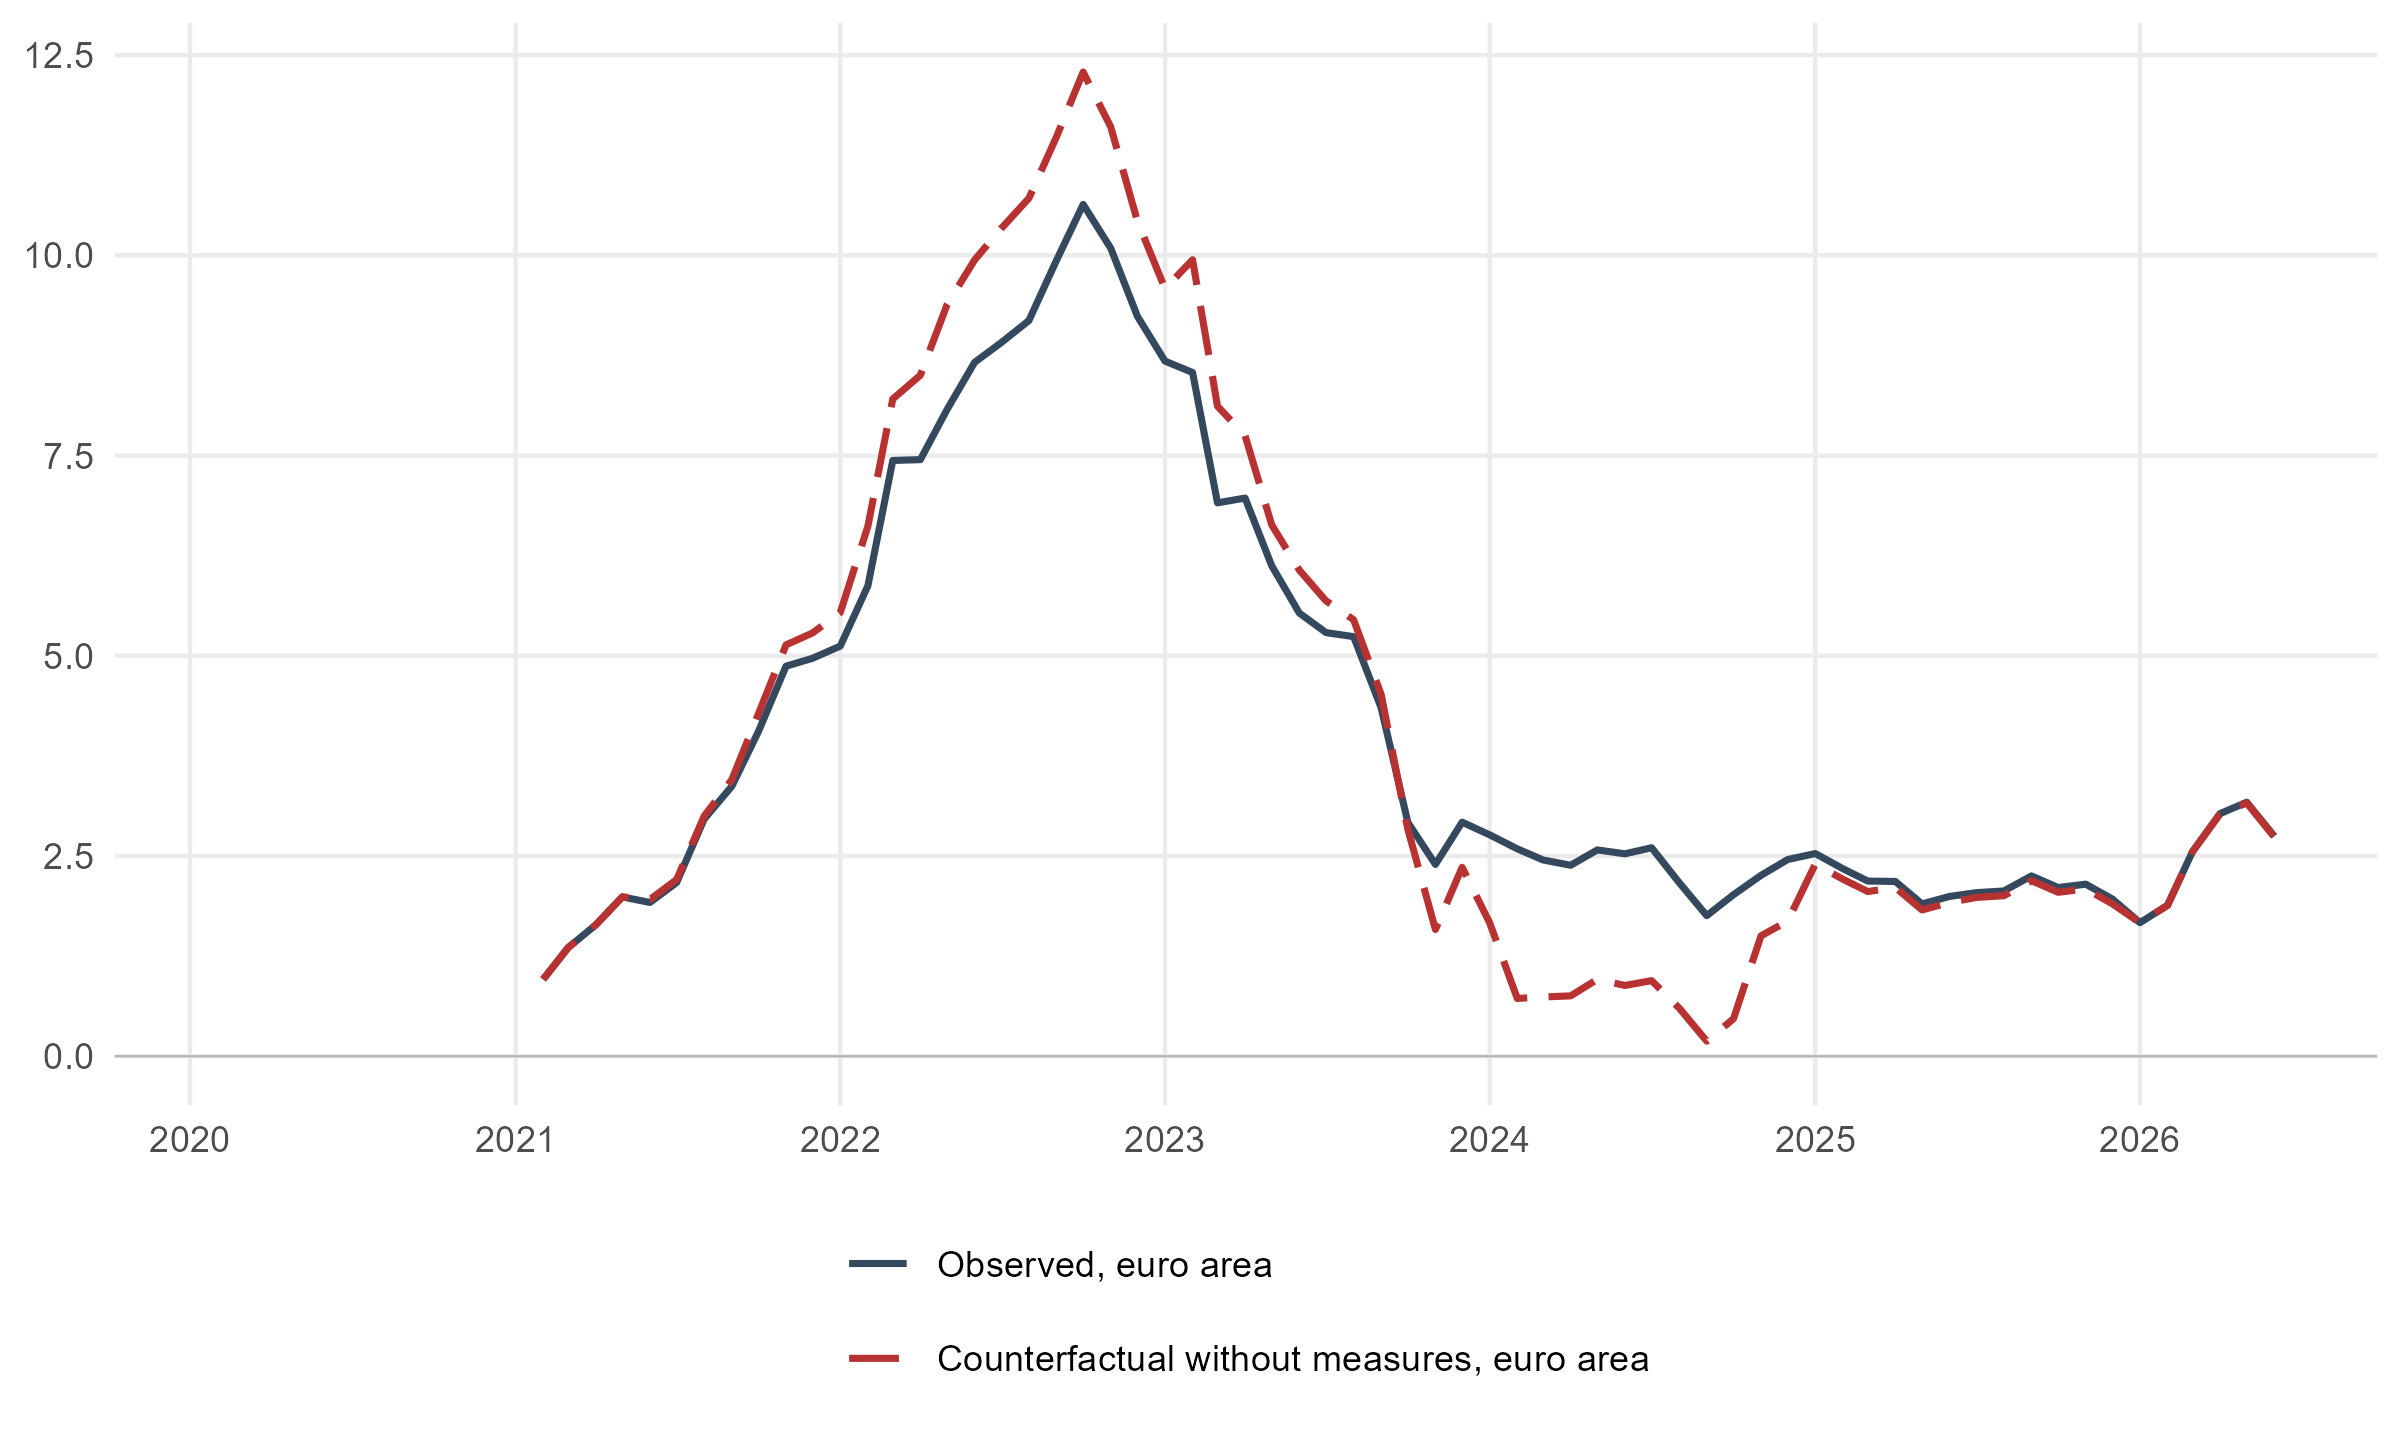
\includegraphics[width=0.86\textwidth,height=0.42\textheight,keepaspectratio]{fig/policy_total_cpi_counterfactual_inflation_EA_policy_sample.png}
\label{fig:ea_policy_total_cpi_counterfactual}
\captionsetup{font=footnotesize, format=hang, singlelinecheck=false, justification=justified}
\caption*{Notes: The no-policy series removes fiscal interventions that directly affected consumer prices. The figure reports year-on-year inflation for all 20 euro-area countries, aggregated with annual HICP country weights, from January 2021 to July 2026. Cumulative inflation is measured between June 2021 and June 2023; the policy effect is defined as observed minus no-policy inflation.\\
Sources: Eurostat HICP; Bruegel energy-policy dataset; authors' calculations.}
\end{figure}

The same timing has a distributional counterpart. Figure~\ref{fig:ea-counterfactual-income-inflation}
shows that, without the price measures, inflation for the first income quintile would have exceeded
that of the fifth quintile by a wider margin during the 2022 peak. The gap subsequently narrowed and
reversed during much of 2024 as energy inflation fell and the earlier policy wedges entered
the year-on-year comparison base. Together with the observed paths in
Figure~\ref{fig:ea20_short_run_income}, this pattern indicates that the measures primarily protected
lower-income households when energy prices were rising fastest. This finding is consistent with
microsimulation evidence that the European fiscal response reduced distributional losses, although
broad price measures were less targeted than income support
\citep{pallotti2024bears,amores2025inflation}.

\begin{figure}[H]
\centering
\caption{Household price policies: no-policy euro-area inflation by income quintile (year on year, in \%)}
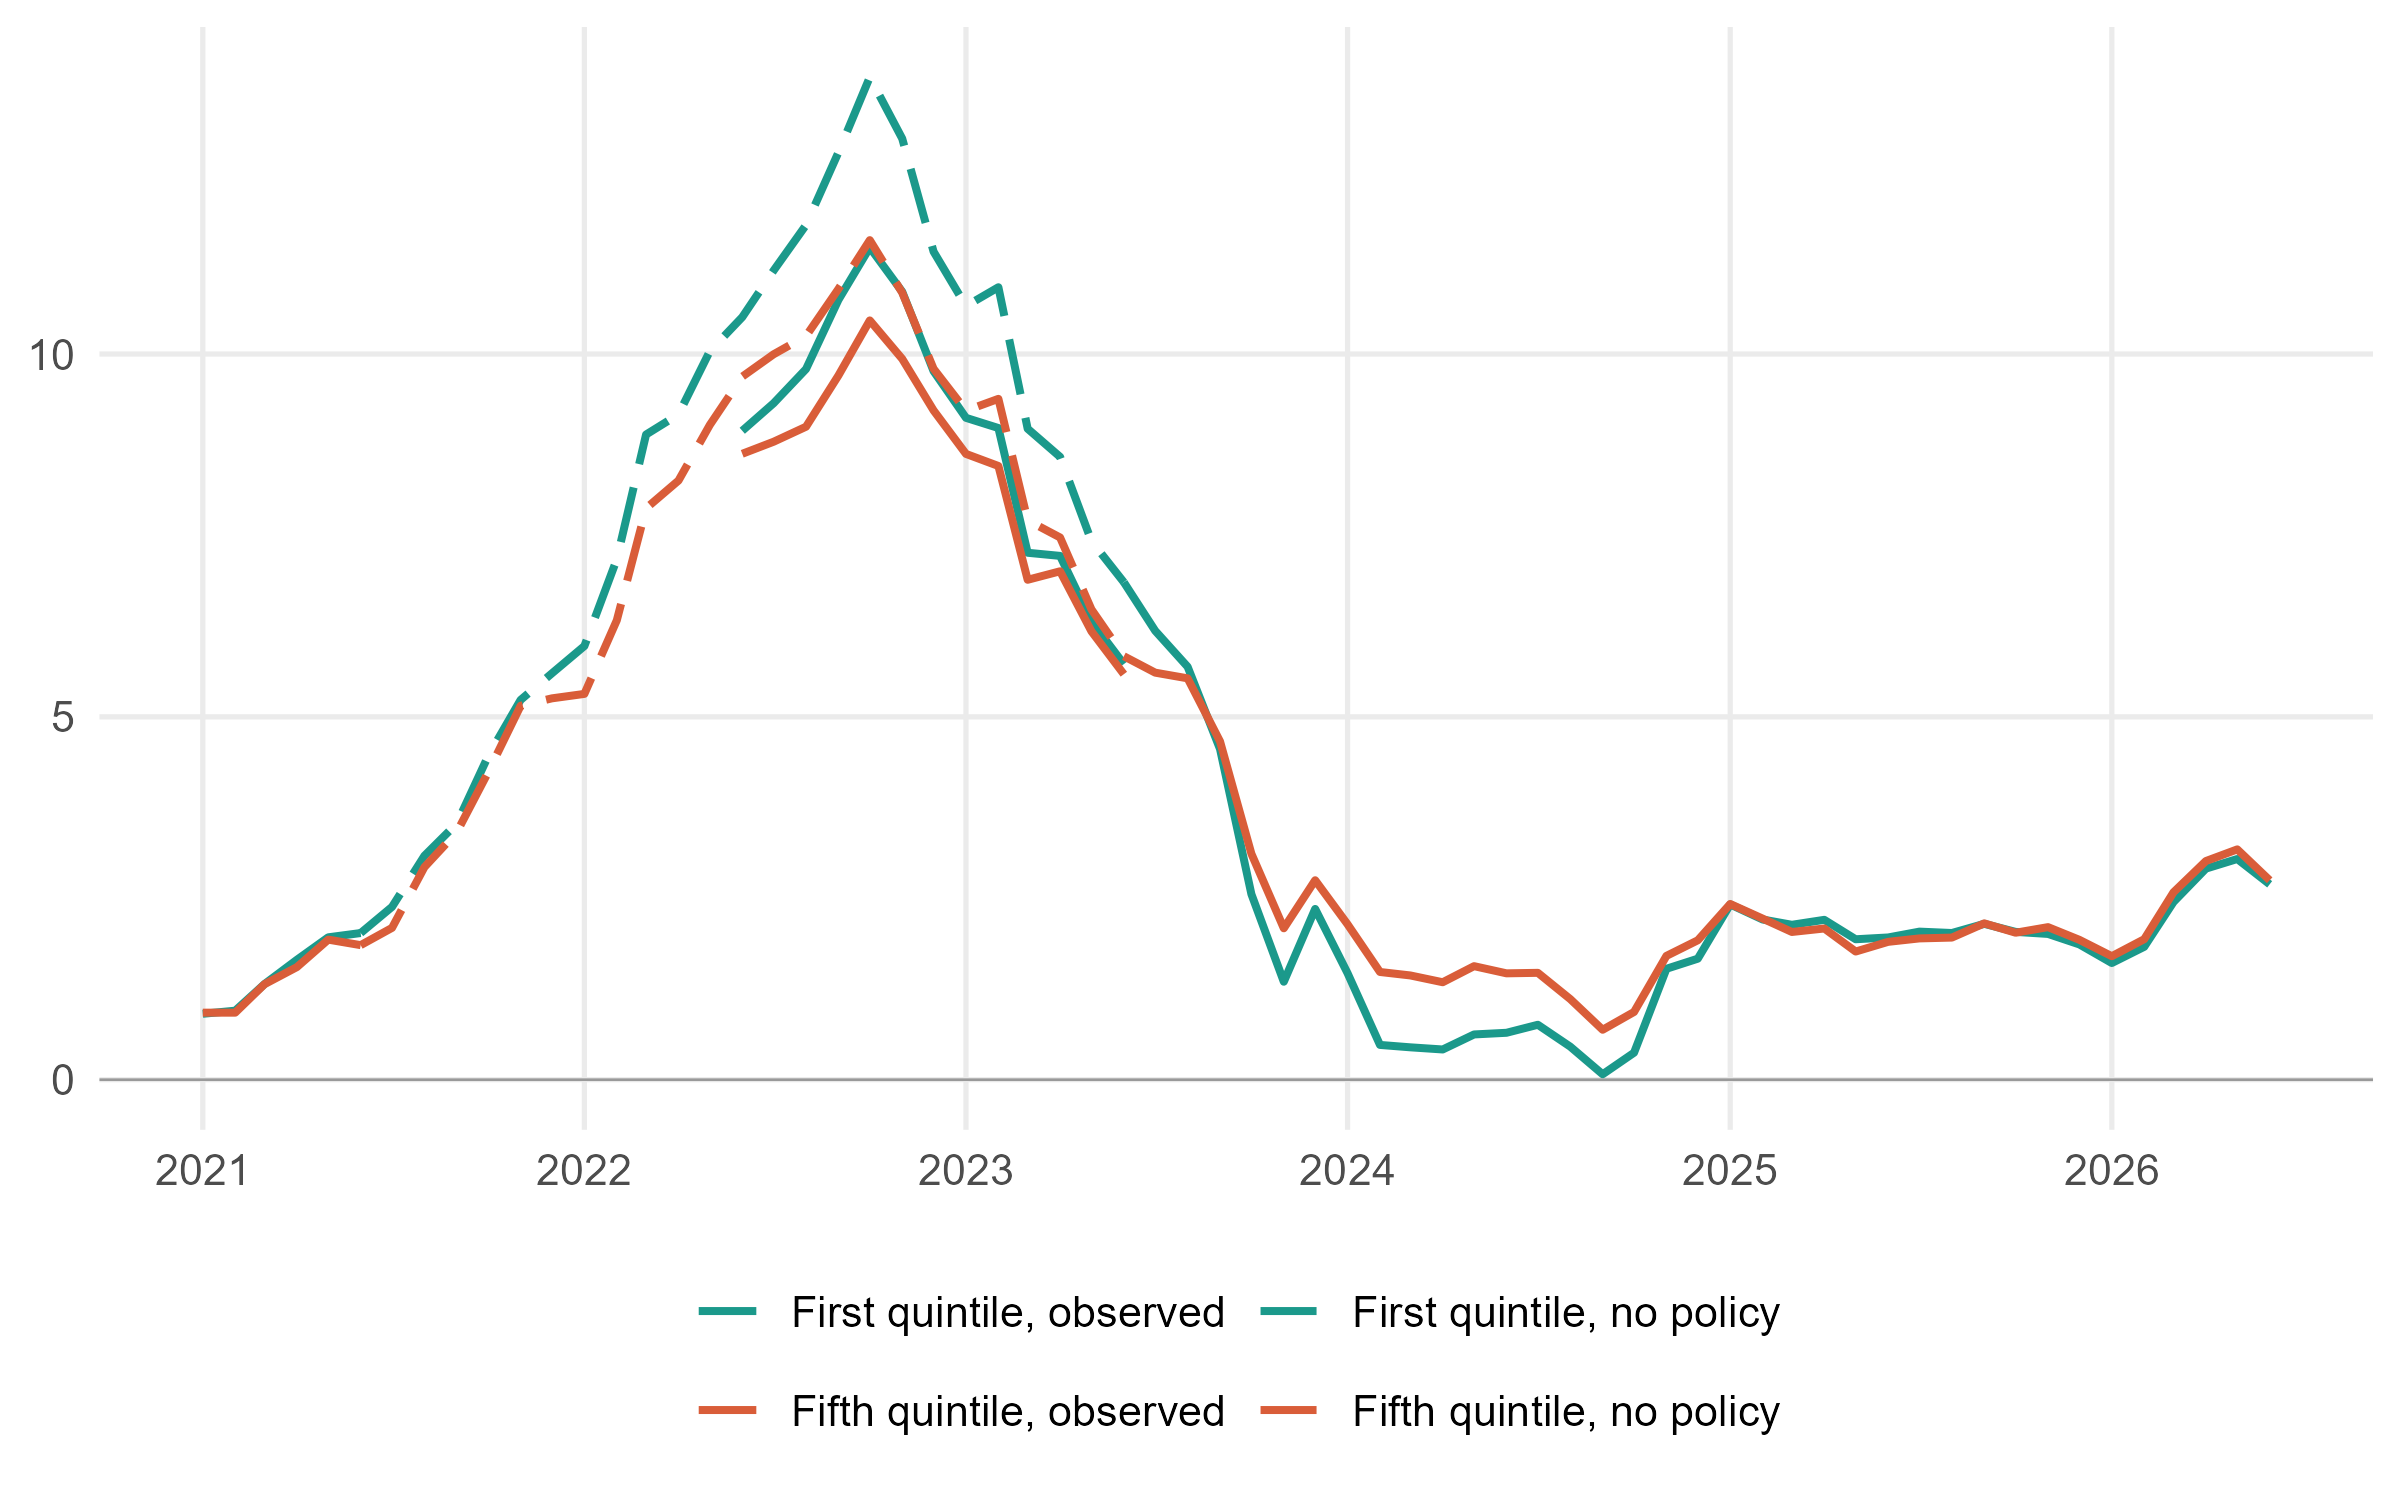
\includegraphics[scale=0.6]{fig/fig_EA20_2021_2026_counterfactual_income_inflation_Q1_Q5.png}
\label{fig:ea-counterfactual-income-inflation}
\captionsetup{font=footnotesize, format=hang, singlelinecheck=false, justification=justified}
\caption*{Notes: The figure reports year-on-year inflation rates in the absence of household price policies for the first and fifth income quintiles,
 from January 2021 to July 2026. Income transfers and firm-only measures are outside the counterfactual. All 20 countries, including Italy and Spain, use RAS expenditure weights and are aggregated using annual HICP country weights.\\
Sources: Eurostat HICP and country weights; household budget surveys; Bruegel energy-policy dataset; authors' calculations.}
\end{figure}

\subsection{Heterogeneity Across Countries and Products}
\label{sec:fiscal-policy-inflation-inequalities}

The aggregate time paths conceal substantial heterogeneity in the effects of the measures. We first
compare countries and then decompose the euro-area effect by product group.

\subsubsection{Differences Across Countries}

Table~\ref{tab:country-heterogeneity-counterfactual-gap} reports the fiscal cost of household price
policies and cumulative no-policy inflation, together with the corresponding income-quintile indices and inflation gap. The
fiscal costs provide context for the scale of the interventions\footnote{These
fiscal costs are not inputs into the price-index counterfactual and do not measure the monetary
benefit received by each household group}. 

%%%%%%%%%%%%%%%%%%%%%%%%%%%%%%%%%%%%%%%%%%%%%%%%%%%%%%%%%%%%%%
\begin{table}[H]
\scriptsize
\setlength{\tabcolsep}{2.5pt}
\renewcommand{\arraystretch}{0.95}

\caption{\label{tab:country-heterogeneity-counterfactual-gap}Household price policies: fiscal cost and no-policy inflation in the 20 euro-area countries, January 2021--December 2023}
\centering
\resizebox{\textwidth}{!}{%
\begin{tabular}{lrrrrrr}
\toprule
Country & \shortstack{Weight\\(2022, \%)} & \shortstack{Fiscal cost\\ (\% of 2022 GDP)} & \shortstack{Counterfactual\\ inflation} & \shortstack{Effect of price policies\\ on average inflation} & \shortstack{Counterfactual\\ inflation gap} & \shortstack{Effect of price policies\\ on inflation inequality}\\
\midrule
Germany & 28.1 & 1.5 & 19.9 & -1.3 & 1.4 & -0.9\\
France & 20.4 & 3.0 & 19.2 & -4.7 & 3.0 & -2.3\\
Italy & 16.3 & 1.8 & 19.5 & -0.8 & 1.6 & -0.3\\
Spain & 11.0 & 1.8 & 19.5 & -3.0 & 1.2 & -1.4\\
Netherlands & 5.4 & 3.5 & 22.7 & -2.6 & 1.8 & -1.2\\
\addlinespace
Belgium & 4.0 & 0.9 & 20.6 & -1.5 & 0.3 & -0.6\\
Austria & 3.3 & 0.9 & 23.4 & -1.4 & 0.3 & -0.7\\
Portugal & 2.2 & 2.4 & 18.1 & -2.7 & 1.0 & -1.4\\
Greece & 2.2 & 4.0 & 19.8 & -1.9 & 2.8 & -1.4\\
Finland & 1.9 & 0.2 & 13.4 & -0.1 & -1.1 & 0.1\\
\addlinespace
Ireland & 1.5 & 0.3 & 18.0 & -0.2 & 4.4 & -0.2\\
Slovakia & 0.8 & 2.1 & 31.8 & -3.4 & 4.3 & -2.2\\
Croatia & 0.7 & 1.3 & 25.5 & -0.7 & 0.1 & -0.5\\
Lithuania & 0.6 & 1.6 & 34.8 & -0.4 & 3.9 & -0.3\\
Slovenia & 0.4 & 0.3 & 21.4 & -0.2 & 1.5 & -0.2\\
\addlinespace
Luxembourg & 0.3 & 1.2 & 15.5 & -1.1 & 0.6 & -0.4\\
Latvia & 0.3 & 1.9 & 31.8 & -1.0 & 6.7 & -0.8\\
Estonia & 0.2 & 0.5 & 36.8 & -0.3 & 6.9 & -0.1\\
Cyprus & 0.2 & 0.7 & 16.0 & 0.0 & 0.3 & 0.0\\
Malta & 0.1 & 4.5 & 17.2 & -1.4 & 1.9 & -0.2\\
\addlinespace
\textbf{Euro area} & \textbf{100.0} & \textbf{2.0} & \textbf{20.0} & \textbf{-2.2} & \textbf{1.8} & \textbf{-1.1}\\
\bottomrule
\end{tabular}%
}
\begin{flushleft}
\footnotesize{Notes. The no-policy counterfactual removes household price policies. Effects are observed minus no-policy values; the gap is Q1 minus Q5. Cumulative changes compare January 2021 with December 2023. Total indices are recomposed from product-country counterfactual prices using official HICP product weights, before national monthly movements are aggregated to EA20 with annual country weights. Fiscal costs are percentages of 2022 nominal GDP; weights are 2022 EA20 HICP shares. Sources: Eurostat, national statistical institutes, Bruegel, national sources, authors' calculations.}
\end{flushleft}
\end{table}

%%%%%%%%%%%%%%%%%%%%%%%%%%%%%%%%%%%%%%%%%%%%%%%%%%%%%%%%%%%%%%

The distributional effects are heterogeneous across countries. Among the countries included in the
euro-area aggregate, the largest reductions in the Quintile 1--Quintile 5 gap are estimated for
France ($-2.2$ points), Slovakia ($-2.1$), Portugal ($-1.5$), Greece ($-1.4$), Spain ($-1.2$),
Lithuania ($-1.1$), and the Netherlands and Germany ($-0.9$ each). Italy has a policy
effect of $-0.3$ point. Estimates close to zero arise either where no policy
layer from Appendix~\ref{sec:app-counterfactuals} enters the country row or where temporary
counterfactual price wedges leave little difference in the June 2021--June 2023 endpoint comparison.
Figure~\ref{fig:ea_policy_total_cpi_counterfactual} and the monthly developments in
Appendix~\ref{sec:app-counterfactuals} complement this cumulative comparison by showing when the
measures affected inflation.

France combines a reported budget of EUR 80.5 billion with a 2.2-point reduction in the
Q1--Q5 inflation gap, whereas Slovakia combines EUR 2.3 billion with a 2.1-point reduction. These
figures refer to economies of different sizes, policy coverage, energy systems, and initial price
exposures. The inflation-gap effect is measured in percentage
points, not as a monetary gain, and it cannot be divided meaningfully by expenditure in euros. A
cost-effectiveness analysis would need household-level policy eligibility, quantities consumed,
tax and transfer rules, and counterfactual expenditures to calculate the fiscal cost and purchasing-
power benefit for each household in a common monetary unit.

\subsubsection{Differences Across Products}

For the euro area, cumulative inflation from the total no-policy HICP index is 16.6 percent.
Counterfactual cumulative inflation is 18.0 percent for Quintile 1 and 16.1 percent for Quintile 5,
compared with observed values of 15.2 and 14.4 percent reported in Table~\ref{tab:country-heterogeneity-cumulative-gap}.
The observed Quintile 1--Quintile 5 gap is therefore 0.9 point, compared with 2.0 points without the
simulated measures. Using unrounded indices, the resulting policy effect is $-1.1$ points.

Table~\ref{tab:ea20-counterfactual-income-gap-product-contributions} reproduces the product-group
decomposition of Table~\ref{tab:ea20-income-gap-product-contributions} using the no-policy paths. It
reports each product group's contribution to cumulative inflation and to the Quintile 1--Quintile 5
gap, together with the effect of the price measures.

%%%%%%%%%%%%%%%%%%%%%%%%%%%%%%%%%%%%%%%%%%%%%%%%%%%%%%%%%%%%%%
\begin{table}[H]
\scriptsize
\setlength{\tabcolsep}{3pt}
\renewcommand{\arraystretch}{0.95}

\caption{\label{tab:ea20-counterfactual-income-gap-product-contributions}Household price policies: product-group contributions to no-policy inflation inequality in the 20-country euro area, June 2021--June 2023}
\centering
\resizebox{\textwidth}{!}{%
\begin{tabular}{lrrrrr}
\toprule
Product group & \shortstack{Counterfactual\\ inflation} & \shortstack{Q1 counterfactual\\ contribution} & \shortstack{Q5 counterfactual\\ contribution} & \shortstack{Counterfactual\\ inflation gap} & \shortstack{Effect of price policies\\ on inflation inequality}\\
\midrule
Food and non-alcoholic beverages & 4.2 & 5.0 & 4.3 & 0.7 & 0.0\\
Alcoholic beverage, tobacco and narcotics & 0.4 & 0.6 & 0.4 & 0.2 & 0.0\\
Clothing and footwear & 0.3 & 0.3 & 0.4 & -0.2 & 0.0\\
Housing (rentals and repairs) & 0.4 & 0.4 & 0.6 & -0.2 & -0.0\\
Water, electricity, gas and other fuels & 7.4 & 10.1 & 7.1 & 3.0 & -1.5\\
\addlinespace
Transport & 2.3 & 1.7 & 3.1 & -1.3 & 0.2\\
Other & 0.3 & 0.2 & 0.4 & -0.1 & 0.0\\
\midrule
\textbf{Total} & \textbf{15.4} & \textbf{18.4} & \textbf{16.3} & \textbf{2.1} & \textbf{-1.2}\\
\bottomrule
\end{tabular}%
}
\vspace{-0.4em}
\begin{flushleft}
\footnotesize{Notes. The no-policy counterfactual replaces prices affected by household price policies and retains other observed prices. The gap is Q1 minus Q5. Policy effects are observed minus no-policy values; negative values indicate that policies reduced the gap. The euro-area aggregate covers all 20 countries using annual HICP country weights. Entries are percentage-point contributions. Totals are calculated before rounding and may differ from the sums of displayed entries. Sources: Eurostat, national statistical institutes, authors' calculations.}
\end{flushleft}
\end{table}

%%%%%%%%%%%%%%%%%%%%%%%%%%%%%%%%%%%%%%%%%%%%%%%%%%%%%%%%%%%%%%

Household energy accounts for the distributional effect. The measures reduce the contribution of
electricity and gas to the Q1--Q5 gap by 1.4 points. Their effect through transport instead increases
the gap by 0.2 point because fuel-price measures also benefit the transport-intensive baskets of
higher-income households; effects through the remaining product groups are close to zero. This
pattern mirrors the input--output simulation: both exercises identify household energy as the main
distributional channel, while transport partly offsets it. The measures thus dampen the direct
exposure that generates most of the energy-shock gap but do less to undo propagation through
production networks.

For comparison, the U.S. distributional CPIs of \citet{jaravel2024distributional} imply cumulative
inflation of 13.0 percent for the first income quintile and 13.5 percent for the fifth between May
2020 and May 2022, a Q1--Q5 gap of $-0.5$ point. The U.S. profile is inverse U-shaped---inflation
reaches 14.7 percent for the middle class---rather than monotonically declining with income. The
sign and size of inflation inequality therefore depend on the composition of the price shock and on
the policies affecting the most exposed products.


\section{Household-Level Inflation}
\label{sec:household-level}

This section moves from inflation indices for broad household groups to estimates constructed from
individual household records. We use the consumption basket reported by each household in the HBS
microdata which we combine with monthly HICP
price indices. This approach show the dispersion within groups and allows us to
examine whether observable household characteristics are systematically associated with inflation
exposure.

%In the empirical application, we use the Spanish EPF, a publicly available HBS microdata source, and match each annual price index to the preceding EPF wave. The HBS survey year is denoted $y'=y-1$ in the expenditure-share formulas below. Household-level inflation is obtained from the price index implied by each household's expenditure shares, and the resulting distributions are weighted using EPF survey weights.

\subsection{Calculating Household Inflation Rates}

We apply fixed-basket Laspeyres at the household level, holding each household's 2020 HBS
basket fixed when calculating inflation for 2021--2023. Let $e^{\mathrm{HBS}}_{i,j,2020}$
denote household $i$'s expenditure on COICOP item $j$ in the 2020 HBS wave, and let $a_{i,2020}$ denote
its survey weight. The household expenditure share is
\begin{equation}
\omega^{\mathrm{HBS}}_{j,i,2020}
=
\frac{a_{i,2020}e^{\mathrm{HBS}}_{i,j,2020}}{\sum_{k \in \mathcal{J}_{i,2020}} a_{i,2020}e^{\mathrm{HBS}}_{i,k,2020}}
=
\frac{e^{\mathrm{HBS}}_{i,j,2020}}{\sum_{k \in \mathcal{J}_{i,2020}} e^{\mathrm{HBS}}_{i,k,2020}}
\end{equation}
using the same convention as the group-specific weights $\omega_{j,g,y}$ defined above. Since the
same survey weight applies to all items within a household, it cancels out in the within-household
basket; it is then used to weight households when constructing cross-household distributions and
summary statistics. For household $i$, the within-year price index in month $m$ of year $y$ is
\begin{equation}
P_{i,y,m}
=
\sum_{j \in \mathcal{J}_{i,2020,y}}
\omega^{\mathrm{HBS}}_{j,i,2020}
\frac{p_{j,y,m}}{p_{j,y,0}}
,
\end{equation}
where $\mathcal{J}_{i,2020,y}$ is the set of household expenditure items observed in the 2020 HBS wave
that can be matched to HICP prices in year $y$. Households are therefore treated as elementary
household groups: the within-year Laspeyres changes are chain-linked at the household level, and
year-on-year monthly inflation rates $\pi_{i,y,m}$ are computed from the resulting chained household
price index.

For each household $i$ in country $c$ and calendar year $y$, average annual inflation is the
arithmetic mean of the 12 monthly year-on-year inflation rates. If $I_{ic,y,m}$ is the chained
household price index, then
\begin{equation}
\pi_{ic,y,m}=100\left(\frac{I_{ic,y,m}}{I_{ic,y-1,m}}-1\right),
\qquad
\bar{\pi}_{ic,y}=\frac{1}{12}\sum_{m=1}^{12}\pi_{ic,y,m}.
\label{eq:average-annual-household-inflation}
\end{equation}
This annual average is the inflation measure used in the household-level regressions and in the
inflation-burden calculation below.

Figure~\ref{fig:ea20-household-inflation-distribution} shows the dispersion of these household-level
inflation rates across the euro-area microdata sample in 2021, 2022, and 2023.

\begin{figure}[H]
\centering
\caption{Distribution of household-level inflation in the euro area, 2021--2023 (in \% of households)}
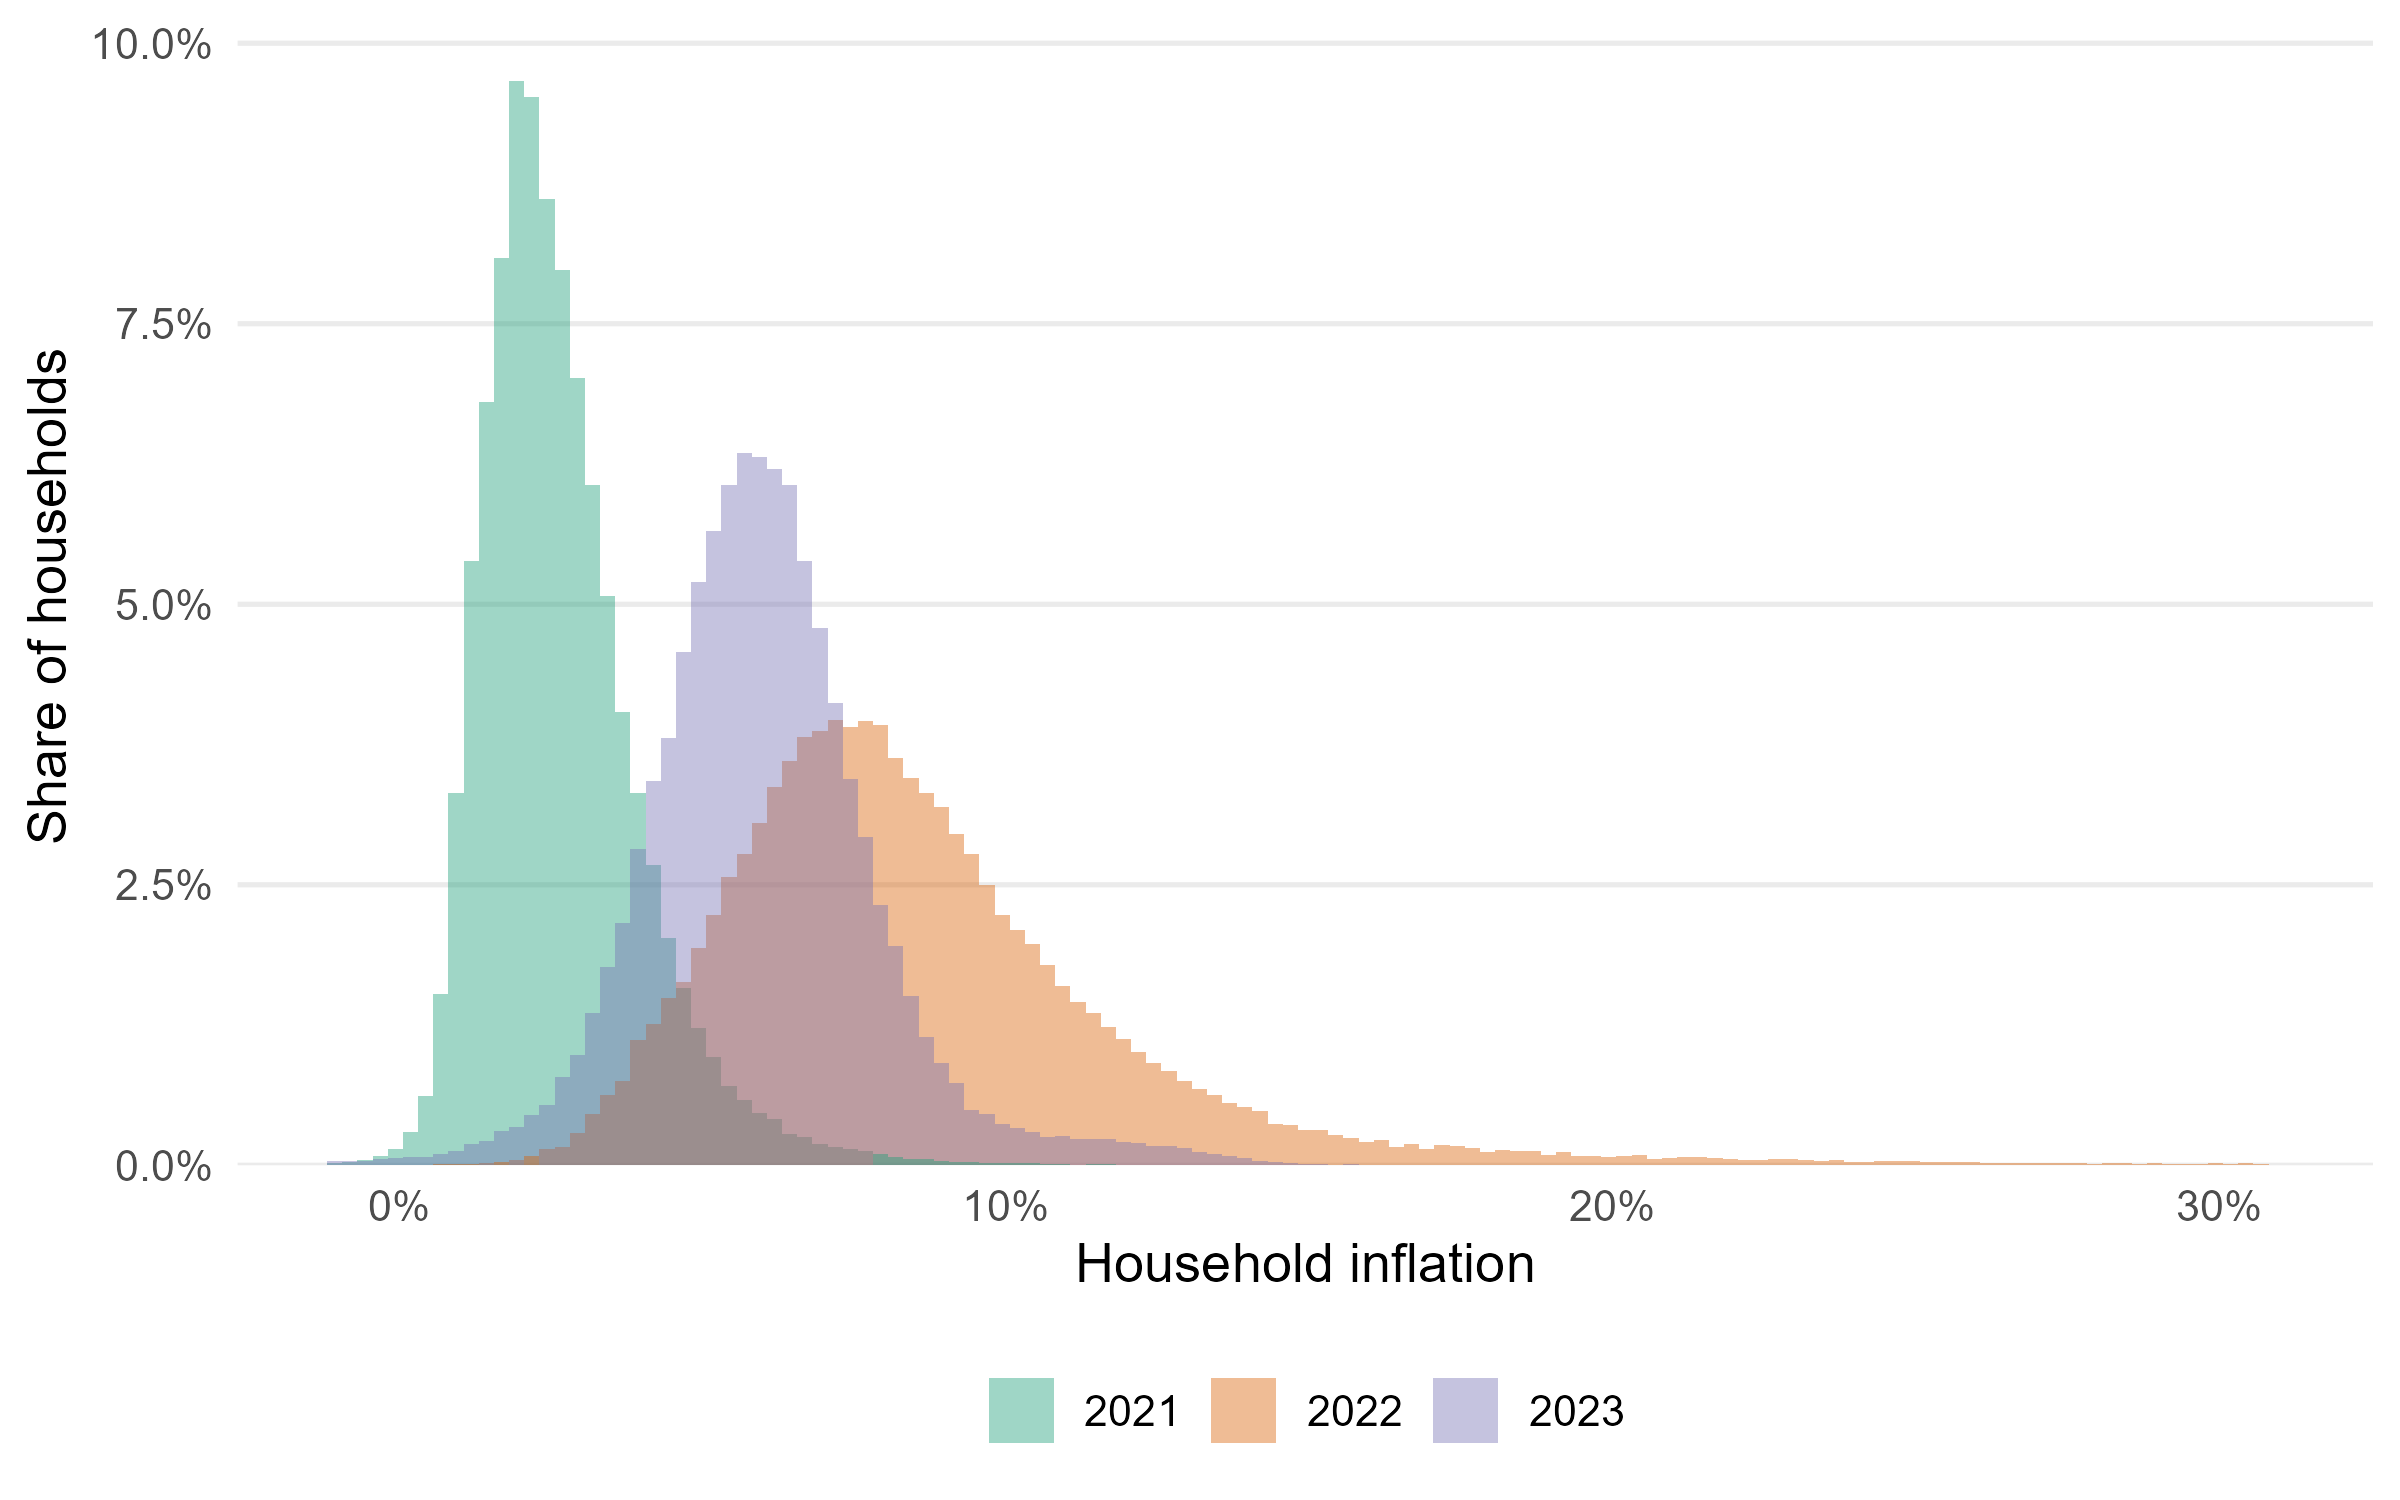
\includegraphics[width=0.86\textwidth,height=0.38\textheight,keepaspectratio]{fig/fig_EA20_household_inflation_distribution_2021_2023.png}
\label{fig:ea20-household-inflation-distribution}
\captionsetup{font=footnotesize, format=hang, singlelinecheck=false, justification=justified}
\caption*{Notes: Histograms report the survey-weighted percentage of households by annual inflation interval, calculated from fixed
2020 household consumption baskets. The displayed range excludes the outer 0.1 percent of the
pooled weighted distribution. The sample covers 19 euro-area countries; Portugal is excluded because
no household basket can be matched to the annual HICP series.\\
Sources: Eurostat HICP and HBS microdata; authors' calculations.}
\end{figure}

%This formula loops over households, product categories, and months. It is more
%computationally demanding than the faster approximation that first aggregates
%item-level annual inflation and then applies household expenditure shares, but
%it is closer to the index construction used for the group-level indicators.

\subsection{Inflation Burden}

Our indicators measure differences in inflation exposure across household groups, but they do
not directly express the cost of inflation relative to household resources. We therefore construct
the burden from HBS microdata rather than combining group-level inflation with an external aggregate
consumption-to-income ratio. For household $i$ in country $c$, let $X_{ic}$ denote total consumption
expenditure, $Y_{ic}$ net household income, and $\bar{\pi}_{ic,y}$ the household's average annual
inflation rate in year $y$, computed from its own COICOP expenditure shares and the corresponding
national HICP price changes. The raw household-level burden is
\begin{equation}
b^{\mathrm{raw}}_{ic,y}=\bar{\pi}_{ic,y}\frac{X_{ic}}{Y_{ic}},
\label{eq:micro-inflation-burden}
\end{equation}
where $\bar{\pi}_{ic,y}$ is measured in percent, so $b^{\mathrm{raw}}_{ic,y}$ is measured in
points of net income. Thus, the indicator allows both individual inflation exposure and
the consumption-to-income ratio to vary across households.

Very small reported incomes can generate mechanically extreme expenditure-to-income ratios. We
therefore winsorize $100X_{ic}/Y_{ic}$ at the survey-weighted 99th percentile within each country,
while retaining the underlying household inflation rate. Denoting the resulting ratio by
$\widetilde{\kappa}_{ic}$, the burden used in the estimates and its aggregation for national income
quintile $q$ are
\begin{equation}
b_{ic,y}=\bar{\pi}_{ic,y}\frac{\widetilde{\kappa}_{ic}}{100},
\qquad
B_{q,y}=\frac{\sum_{c}\sum_{i\in q(c)}a_{ic}b_{ic,y}}
{\sum_{c}\sum_{i\in q(c)}a_{ic}},
\label{eq:aggregate-micro-inflation-burden}
\end{equation}
where $a_{ic}$ is the HBS survey weight and $q(c)$ indicates that equivalized-income quintiles are
defined separately within each country before households are pooled. The survey weights expand the
microdata to national household populations and therefore determine the euro-area aggregation.
The 2020 HBS basket, income, and expenditure observations are held fixed, while household-specific
inflation is calculated for 2021--2023. For each household-year, the inflation rate is computed over
the expenditure categories matched to available HICP items and the matched shares are renormalized
to one. We impose no minimum matched-expenditure threshold.

Higher-income households also generally have greater capacity to absorb a price
shock by reducing discretionary expenditure or substituting toward cheaper varieties. Appendix
Figure~\ref{fig:app-ea-essentials-discretionary} documents the corresponding difference in basket
composition.

Figure~\ref{fig:ea20-inflation-burden} reports the weighted household-level burden. The first
quintile faces a substantially larger burden in every year: 3.1 percent of net income in 2021,
10.2 percent in 2022, and 7.4 percent in 2023, compared with 2.0, 5.7, and 4.1 percent for the fifth
quintile. The Q1--Q5 burden gap therefore widened from 1.1 points in 2021 to 4.5 points at the peak
of the energy-price shock in 2022, before narrowing to 3.3 points in 2023.

\begin{figure}[H]
\centering
\caption{Household-level inflation burden in the euro area, by income quintile (in \% of net income)}
\label{fig:ea20-inflation-burden}
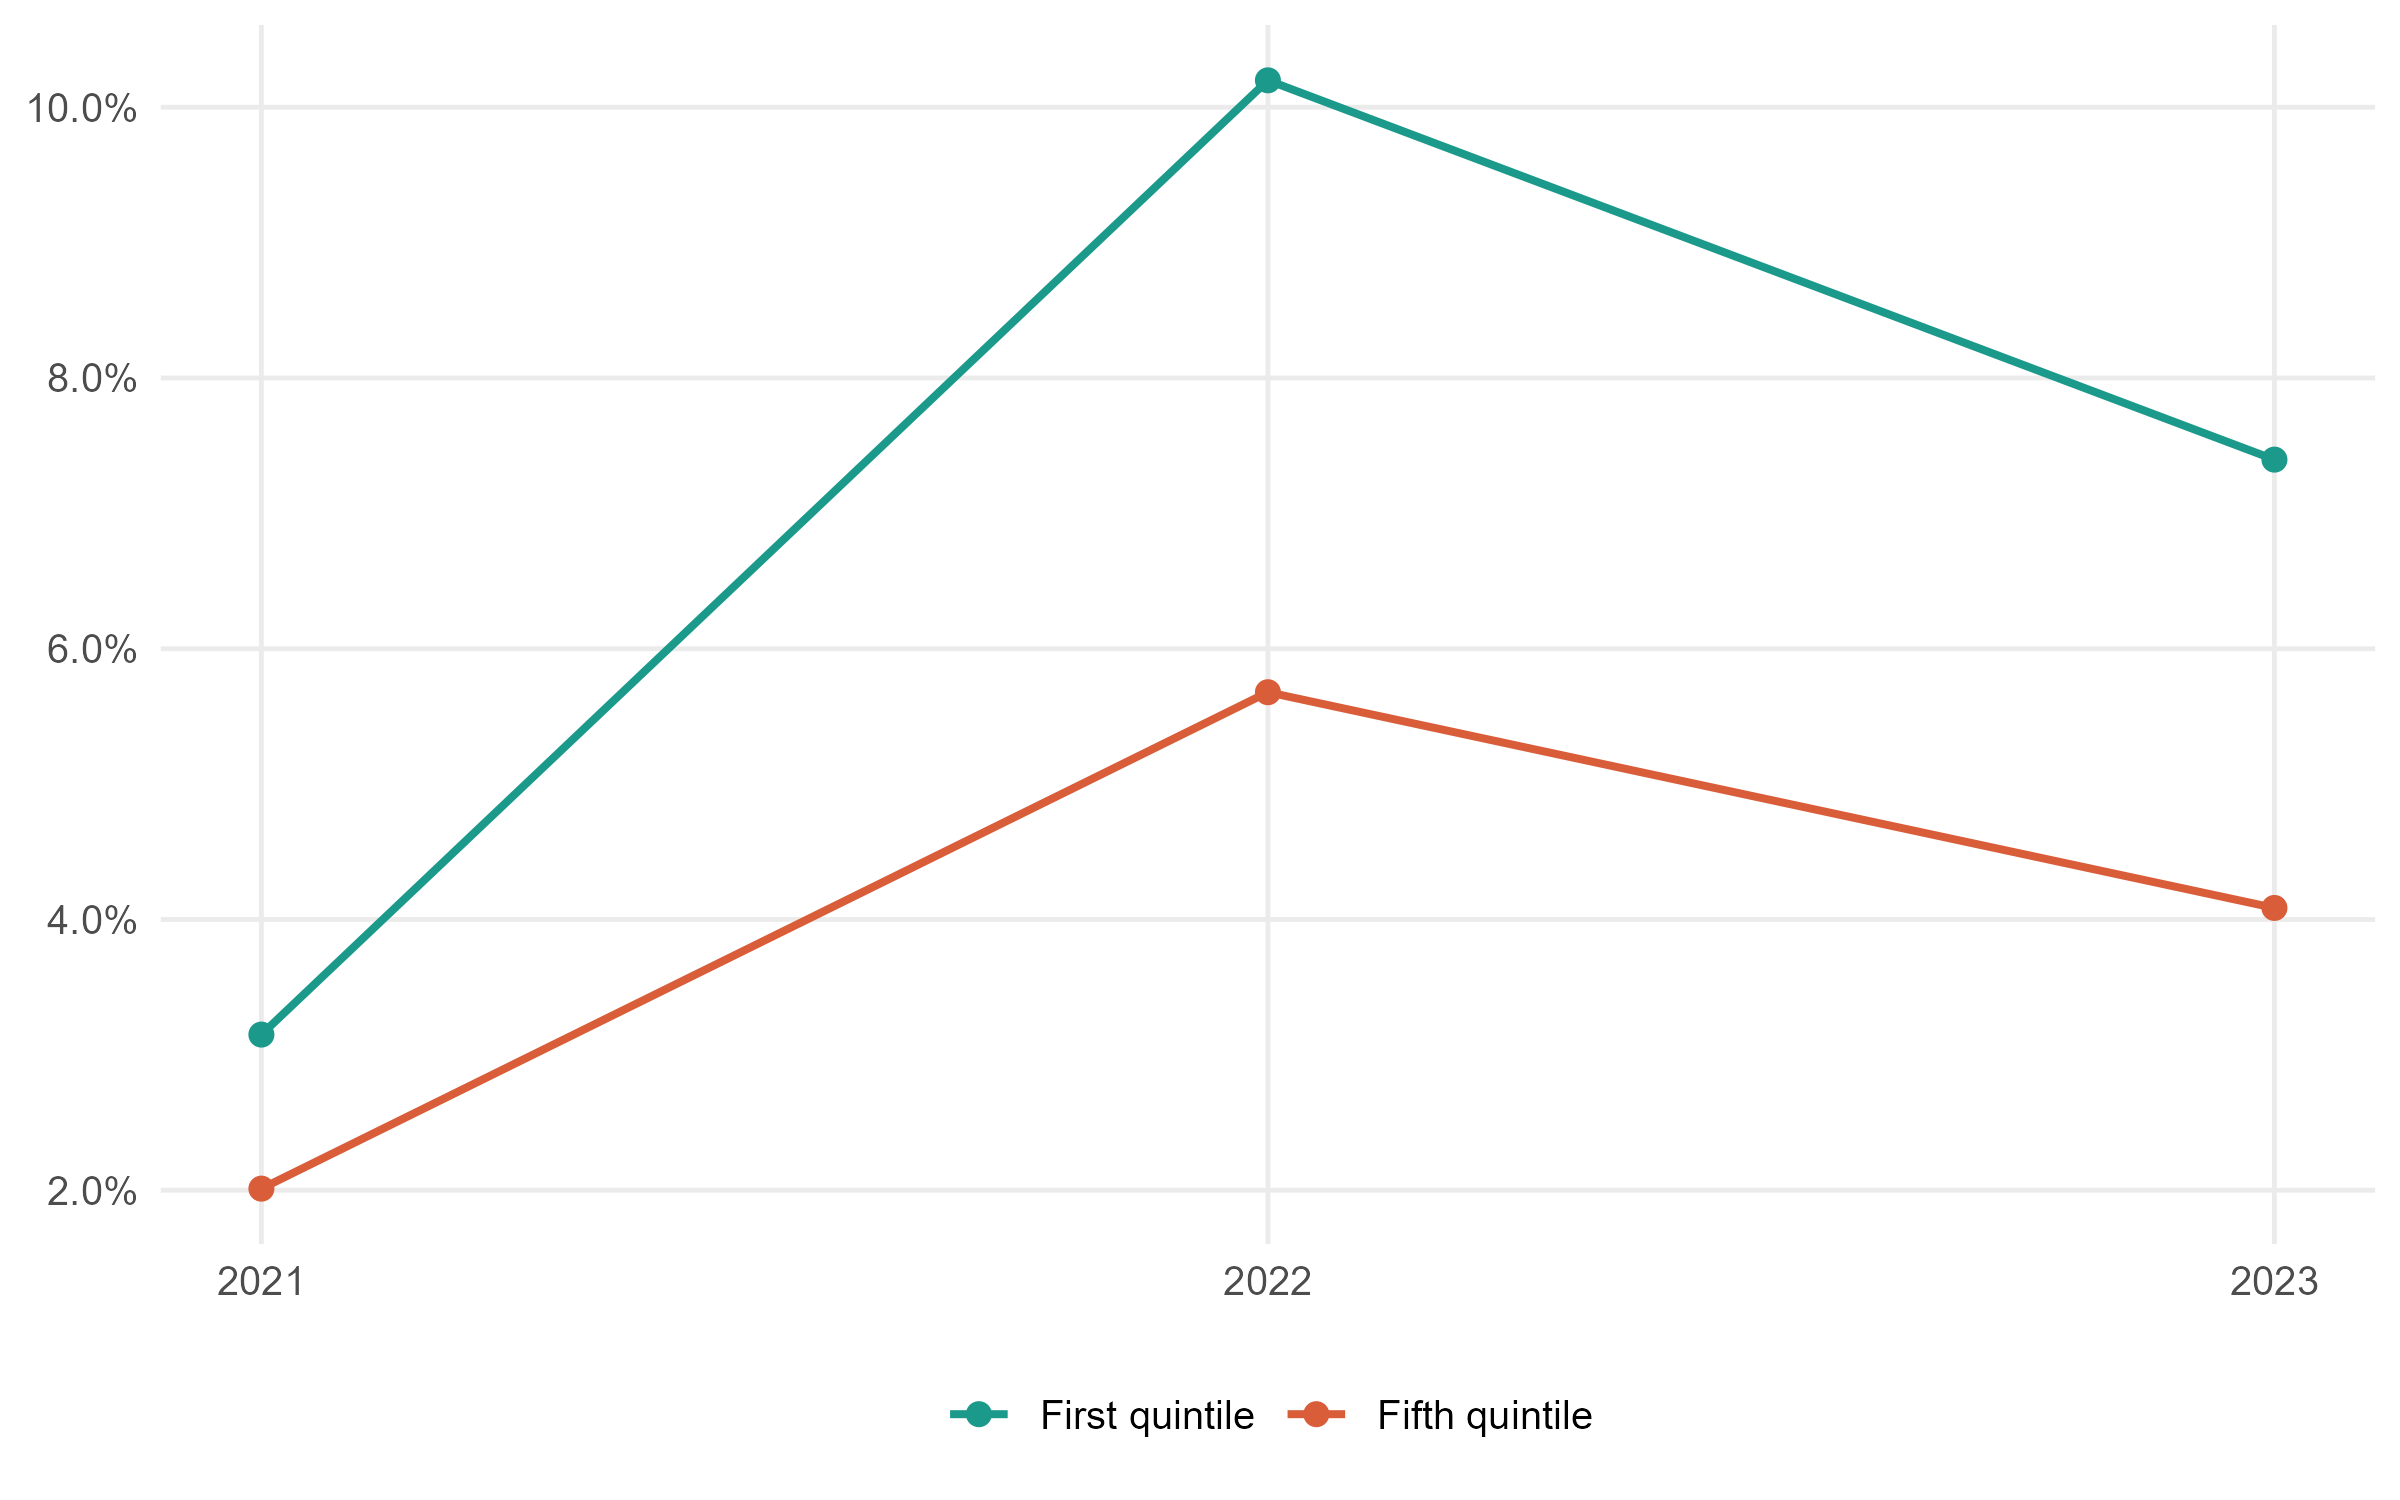
\includegraphics[width=0.78\textwidth,height=0.31\textheight,keepaspectratio]{fig/fig_EA20_2019_2026_income_inflation_burden_Q1_Q5.png}
\vspace{4pt}
\captionsetup{font=footnotesize, format=hang, singlelinecheck=false, justification=justified}
\caption*{Notes: The burden is computed for each household as its annual basket-specific inflation rate multiplied by its consumption-to-net-income ratio. Ratios are winsorized at the survey-weighted national 99th percentile; income quintiles are defined within countries. Estimates use the 2020 HBS microdata and annual inflation for 2021--2023. Italy is excluded because the harmonized micro-income input is unavailable. Portugal is absent because no household basket can be matched to the annual HICP series. The resulting sample covers 18 euro-area countries.\\
Sources: Eurostat HICP and HBS microdata; authors' calculations.}
\end{figure}


\subsection{Household Characteristics and Inflation Exposure}

We pool individual household records from the euro area to examine whether
differences in consumption baskets translate into systematic differences in inflation exposure.
We examine how income quintile, age, household size, and degree of urbanization are associated with
household-specific inflation.

Table~\ref{tab:hbs-inflation-regressions-by-year}
reports separate regressions for 2021, 2022, and 2023, with country fixed effects.
Table~\ref{tab:hbs-inflation-regressions-pooled} pools the three years and includes both country and
year fixed effects. Hence, the coefficients capture conditional differences between households
within countries, net of the included characteristics and common country effects; the pooled
estimates additionally net out the large common changes in inflation across years. They should be
interpreted as descriptive conditional associations, not as causal effects.

\begin{table}[H]
\centering
\caption{Household-level inflation regressions by year, euro-area sample}
\label{tab:hbs-inflation-regressions-by-year}
\scriptsize
\setlength{\tabcolsep}{3pt}
\renewcommand{\arraystretch}{0.9}

\begingroup
\centering
\begin{tabular}{lccc}
   \tabularnewline \midrule \midrule
   Dependent Variable: & \multicolumn{3}{c}{mean\_inflation}\\
   Year                   & 2021            & 2022            & 2023 \\   
   Model:                 & (1)             & (2)             & (3)\\  
   \midrule
   \emph{Variables}\\
   Less than 30 years     & -0.1692         & -2.005$^{***}$  & -0.6680$^{**}$\\   
                          & (0.1129)        & (0.2119)        & (0.2426)\\   
   From 30 to 44 years    & -0.0156         & -1.391$^{***}$  & -0.5693$^{***}$\\   
                          & (0.0844)        & (0.1612)        & (0.0890)\\   
   From 45 to 59 years    & 0.0140          & -0.8904$^{***}$ & -0.2963$^{***}$\\   
                          & (0.0892)        & (0.1706)        & (0.0771)\\   
   Income quintile 2      & 0.1113$^{*}$    & -0.6340$^{**}$  & -0.1970$^{**}$\\   
                          & (0.0602)        & (0.2379)        & (0.0737)\\   
   Income quintile 3      & 0.1693          & -0.6450$^{**}$  & -0.1542\\   
                          & (0.1142)        & (0.2551)        & (0.0905)\\   
   Income quintile 4      & 0.2371$^{*}$    & -0.6881$^{***}$ & -0.1698$^{*}$\\   
                          & (0.1362)        & (0.2367)        & (0.0962)\\   
   Income quintile 5      & 0.3104$^{*}$    & -0.8511$^{***}$ & -0.2247$^{**}$\\   
                          & (0.1562)        & (0.2391)        & (0.1008)\\   
   Household size         & 0.0209          & -0.0696         & 0.1153$^{***}$\\   
                          & (0.0415)        & (0.0800)        & (0.0389)\\   
   Intermediate area      & -0.2723$^{***}$ & -0.7404$^{***}$ & 0.0201\\   
                          & (0.0809)        & (0.1223)        & (0.0456)\\   
   Densely populated area & -0.6118$^{***}$ & -1.432$^{***}$  & -0.0360\\   
                          & (0.0979)        & (0.1364)        & (0.1197)\\   
   \midrule
   \emph{Fixed-effects}\\
   country                & Yes             & Yes             & Yes\\  
   \midrule
   \emph{Fit statistics}\\
   Observations           & 152,438         & 152,440         & 152,440\\  
   R$^2$                  & 0.31975         & 0.66935         & 0.63879\\  
   Within R$^2$           & 0.04698         & 0.09037         & 0.02904\\  
   \midrule \midrule
   \multicolumn{4}{l}{\emph{Clustered (country) standard-errors in parentheses}}\\
   \multicolumn{4}{l}{\emph{Signif. Codes: ***: 0.01, **: 0.05, *: 0.1}}\\
\end{tabular}
\par\endgroup



\vspace{4pt}
\captionsetup{font=footnotesize, format=hang, singlelinecheck=false, justification=justified}
\caption*{\emph{Notes:} The dependent variable is mean annual household inflation, in percent. Regressions are estimated separately by inflation year using household survey weights and include country fixed effects. The omitted categories are income quintile 1 and rural areas. The estimation sample covers 18 euro-area countries; Italy lacks usable harmonized household income and Portugal has no household basket that can be matched to the annual HICP series. Standard errors clustered by country are reported in parentheses.\\
\emph{Sources:} Household Budget Survey microdata; Eurostat HICP; authors' calculations.}
\end{table}

All three regressions use household records from the same 2020 HBS wave and impose no minimum
matched-expenditure threshold. Annual inflation can nevertheless be calculated only when at least
one category in a household's basket matches an HICP item with sufficient monthly price coverage.
After removing the matching threshold, the estimation sample contains 152,438 observations in 2021
and 152,440 in both 2022 and 2023. Only two regression observations therefore lack sufficient price
matches in 2021. The effective estimation sample is otherwise constant across years.

\begin{table}[H]
\centering
\caption{Pooled household-level inflation regression, euro-area sample}
\label{tab:hbs-inflation-regressions-pooled}
\scriptsize
\setlength{\tabcolsep}{3pt}
\renewcommand{\arraystretch}{0.9}

\begingroup
\centering
\begin{tabular}{lc}
   \tabularnewline \midrule \midrule
   Dependent Variable:    & mean\_inflation\\   
   Model                  & Pooled \\   
   Model:                 & (1)\\  
   \midrule
   \emph{Variables}\\
   Less than 30 years     & -0.9546$^{***}$\\   
                          & (0.1083)\\   
   From 30 to 44 years    & -0.6742$^{***}$\\   
                          & (0.0660)\\   
   From 45 to 59 years    & -0.3961$^{***}$\\   
                          & (0.0782)\\   
   Income quintile 2      & -0.2793$^{**}$\\   
                          & (0.1166)\\   
   Income quintile 3      & -0.2369$^{*}$\\   
                          & (0.1335)\\   
   Income quintile 4      & -0.2369$^{*}$\\   
                          & (0.1295)\\   
   Income quintile 5      & -0.2860$^{**}$\\   
                          & (0.1354)\\   
   Household size         & 0.0266\\   
                          & (0.0460)\\   
   Intermediate area      & -0.3333$^{***}$\\   
                          & (0.0536)\\   
   Densely populated area & -0.6906$^{***}$\\   
                          & (0.0764)\\   
   \midrule
   \emph{Fixed-effects}\\
   country                & Yes\\  
   year                   & Yes\\  
   \midrule
   \emph{Fit statistics}\\
   Observations           & 439,512\\  
   R$^2$                  & 0.62133\\  
   Within R$^2$           & 0.02448\\  
   \midrule \midrule
   \multicolumn{2}{l}{\emph{Clustered (country) standard-errors in parentheses}}\\
   \multicolumn{2}{l}{\emph{Signif. Codes: ***: 0.01, **: 0.05, *: 0.1}}\\
\end{tabular}
\par\endgroup



\vspace{4pt}
\captionsetup{font=footnotesize, format=hang, singlelinecheck=false, justification=justified}
\caption*{\emph{Notes:} The dependent variable is mean annual household inflation, in percent. The regression uses household survey weights and includes country and inflation-year fixed effects. The omitted categories are income quintile 1 and rural areas. The estimation sample covers 18 euro-area countries; Italy lacks usable harmonized household income and Portugal has no household basket that can be matched to the annual HICP series. Standard errors clustered by country are reported in parentheses.\\
\emph{Sources:} Household Budget Survey microdata; Eurostat HICP; authors' calculations.}
\end{table}

The income-quintile coefficients change sign over time. Relative to the first quintile, households in the upper
quintiles experienced higher inflation in 2021: the coefficients rise from 0.11 point for
the second quintile to 0.31 point for the fifth. In 2022, all four coefficients are
negative and statistically significant, ranging from $-0.63$ to $-0.85$ points, with the
largest difference for the fifth quintile. The coefficients remain negative in 2023, between
$-0.15$ and $-0.22$ points; three of the four are statistically different from zero at the 10 percent
level. In the pooled specification, they range from $-0.21$ to $-0.26$ point. The second-quintile
coefficient is significant at 5 percent and the fifth-quintile coefficient at 10 percent, whereas
the middle-quintile coefficients are not statistically different from zero. Thus, higher-income households had
slightly higher inflation in 2021 but lower inflation during 2022--23; the results do not support a
stable linear relationship between income rank and household inflation over the full period.

Age differences are largest during the energy-price shock. Relative to households whose reference
person is aged 60 or over, households under 30 experienced 2.01 points lower inflation in
2022 and 0.67 point lower inflation in 2023. The corresponding differences for households
aged 30--44 were $-1.39$ and $-0.57$ points, and those for households aged 45--59 were
$-0.89$ and $-0.30$ points. The pooled coefficients preserve this age gradient, ranging
from $-0.40$ point for ages 45--59 to $-0.95$ point for households under 30.

Household size is also associated with inflation exposure, but its sign varies across years. Each
additional household member is associated with 0.02 point higher inflation in 2021,
0.07 point lower inflation in 2022, and 0.12 point higher inflation in 2023.
The pooled estimate is positive but small, at 0.02 point. This instability suggests that
household size mainly proxies for differences in baskets whose inflation sensitivity depends on the
composition of the shock, rather than a persistent exposure gradient.

Residence differences are concentrated in 2021--22. Conditional on the other covariates and country
effects, inflation in 2022 is estimated to be 0.74 point lower in intermediate-density
areas and 1.43 points lower in densely populated areas than in rural areas. In 2023, the
differences narrow to 0.02 point higher inflation in intermediate areas and 0.04 point
lower inflation in densely populated areas. The pooled estimates are respectively $-0.33$ and
$-0.69$ point. The large 2022 gaps are consistent with rural households allocating larger
shares to home energy and private transport, the categories most exposed to the energy-price shock.

\section{Conclusion}


%This paper a set of public indicators to measure inflation inequalities in real-time monthly 
%across socio-demographic groups in the Euro Area.

%Inflation inequality during the 2021--2023 episode varied more across countries, age groups, and
%residence areas than across income quintiles in the euro-area aggregate. 

This paper constructs indicators to measure inflation inequalities  
across socio-demographic groups in the euro area. Between June 2021 and June 2023,
 the cumulative Quintile 1--Quintile 5 gap was 0.9 point, compared with 1.3 points between
households aged 60 or over and those under 30, and 1.0 point between rural and urban households.
These differentials are concentrated around the energy-price surge and narrowed as energy
inflation receded. Inflation inequalities remain limited in a low-inflation environment.

Similar average inflation rates nevertheless imposed sharply different burdens. In 2022, inflation
absorbed 10.2 percent of net income for households in the first income quintile, compared with 5.7
percent for those in the fifth. Household characteristics also mattered. Age and residence show
the largest conditional differences during the energy shock: the rural--urban gradient is pronounced
in 2021--22 but vanishes in 2023, while the age gradient persists through 2023. Income and household
size display less stable relationships across years. VAT reductions, fuel rebates, and energy price shields
lowered average cumulative inflation by 1.9 points and reduced the aggregate Quintile 1--Quintile 5
gap by 1.1 points in the no-policy comparison.

In the policy counterfactual,
lower household-energy prices reduce the Q1--Q5 gap by 1.4 points, while lower transport prices
increase it by 0.2 point. Unconventional fiscal measures were therefore distributionally
effective mainly because they targeted the retail energy prices to which lower-income households
were directly exposed. These measures had little effect on price increases transmitted through
firms' input costs.

%Consumption-based inflation inequality captures only one dimension of the distributional effects of inflation. A complete assessment also requires accounting for income indexation, transfers, and wealth effects, which may dominate consumption-basket effects for some households \citep{cardoso2022heterogeneous,pallotti2024bears}.

Income alone does not identify vulnerable households: residence and age also capture
differences in heating technology, mobility constraints, and the ability to substitute between
products. More granular transaction and expenditure data would allow future work to measure substitution
within product categories.

In the euro area, price-based fiscal measures temporarily cushioned the distributional effects of the 2021--2023 inflation surge, 
while the subsequent disinflation unfolded alongside monetary tightening aimed at restoring aggregate price stability.
Recent fiscal measures reduced inflation inequality in the euro area, while assessing the distributional
 effects of monetary policy lies beyond the scope of this paper (\cite{ampudia2024shopping}).

An extension of this article would combine household-specific price indices with harmonized euro-area household balance-sheet surveys 
to assess the heterogeneous effects of inflation on household wealth, particularly across debtors and creditors and across 
households with different asset and liability compositions.

%

%A household tax-benefit and energy-consumption microsimulation could also allocate
%the fiscal cost of each measure across the distribution and convert the associated purchasing-power
%gains into euros. This extension would permit genuine cost-effectiveness comparisons across policy
%instruments and countries; the budget totals and inflation-gap effects reported here cannot provide
%such a ranking on their own. Such an integrated approach would sharpen the central lesson of our results:
%aggregate inflation can conceal large differences in the loss of household purchasing power.


%The indicators remain subject to aggregation bias and exclude income and wealth channels. More
%granular scanner, transaction, and household expenditure data would improve measurement within broad
%consumption categories and household groups.

%Granular data make it possible to take into account the income channels, wage indexation to inflation, as well as wealth effects. \cite{cardoso2022heterogeneous} show that in Spain, the distributional effects of inflation through household wealth and income outweigh those arising from consumption patterns. Similarly, \cite{pallotti2024bears} find that net household wealth is the primary driver of inflation inequality across six euro area countries (Germany, France, Italy, Spain, the Netherlands, and Belgium). Their findings highlight that older households are disproportionately affected, primarily due to the adverse impact of inflation on their wealth.

%policy implications
%The heterogeneous impact of inflation across household categories suggests the need for carefully calibrated policy responses. While monetary policy remains the primary tool for controlling aggregate inflation, targeted fiscal measures may be necessary to address acute distributional concerns during periods of elevated inflation.

%Understanding the heterogeneous effects of inflation is crucial to design policies that support vulnerable households face inflationary shocks. While fiscal policy can provide temporary relief, only monetary policy can bring inflation back to target in the long run.
%Monetary policy channel of transmission have lags. What role should fiscal measures in the short run, such as targeted VAT reductions, play in mitigating inflation for the most vulnerable households?

%Possible Extensions Possible extension of this paper for the Euro Area could be first non-homothetic price indices that allows for a more accurate representation of consumption patterns across income groups (Jaravel and Lashkari 2023). S


%Fiscal policy can best contribute to mitigating the negative impact of inflation on households through targeted and temporary support measures (tariff protection, increases in pensions and social benefits).

% These measures must be temporary; fiscal policy is not intended to combat inflation, particularly in indebted countries. Monetary and fiscal policies each have a role to play in addressing the consequences of high inflation. In the long run, only monetary policy is effective in bringing inflation back to its target.


% Bibliographie

 \bibliographystyle{ecta}
 \bibliography{references}
\nocite{*}


\clearpage

\appendix
\renewcommand{\thesection}{\Alph{section}}

%%%%%%%%%%%%%%%%%%%%%%%%%%%%%%%%%%%%%%%%%   APPENDIX  -- SETTING COUNTERS TO ZERO
\setcounter{figure}{0}
\setcounter{table}{0}

% \renewcommand{\thesubsection}{\arabic{subsection})}
%\renewcommand{\thetable}{\Roman{table}}
%\renewcommand{\thefigure}{\Roman{figure}}
\counterwithin{figure}{section}
\counterwithin{table}{section}
\renewcommand{\thefigure}{\Alph{section}.\arabic{figure}}
\renewcommand{\thetable}{\Alph{section}.\arabic{table}}

%\pagenumbering{roman}
 \setcounter{page}{1}
\begin{center}

{\textbf{\Large  Appendix     \\ }}\vspace{0.3cm}
\Large {Erwan Gautier - Jérémi Montornès} \\
\vspace{1cm}
{\Large(Not for publication)}\\
\vspace{1cm}
\today\\



\end{center}




%\addcontentsline{toc}{section}{Annexes}

%\renewcommand{\thetable}{\Alph{section}}
%\renewcommand{\thefigure}{\Alph{section}}

\section{Additional Figures on the Household Budget Surveys}
\label{sec:app-additional-hbs-figures}





%%%%%%%%%%%%%%%%%%%%%%%%%%%%%%%%%%%%%%%%%%%%%%%%%%%%%%%%%%%%%%
\begin{figure}[H]
\centering
\caption{Main COICOP expenditure weights by income quintile, Spain (in \% of total expenditure)}
\label{fig:app-es-income-coicop-weights}
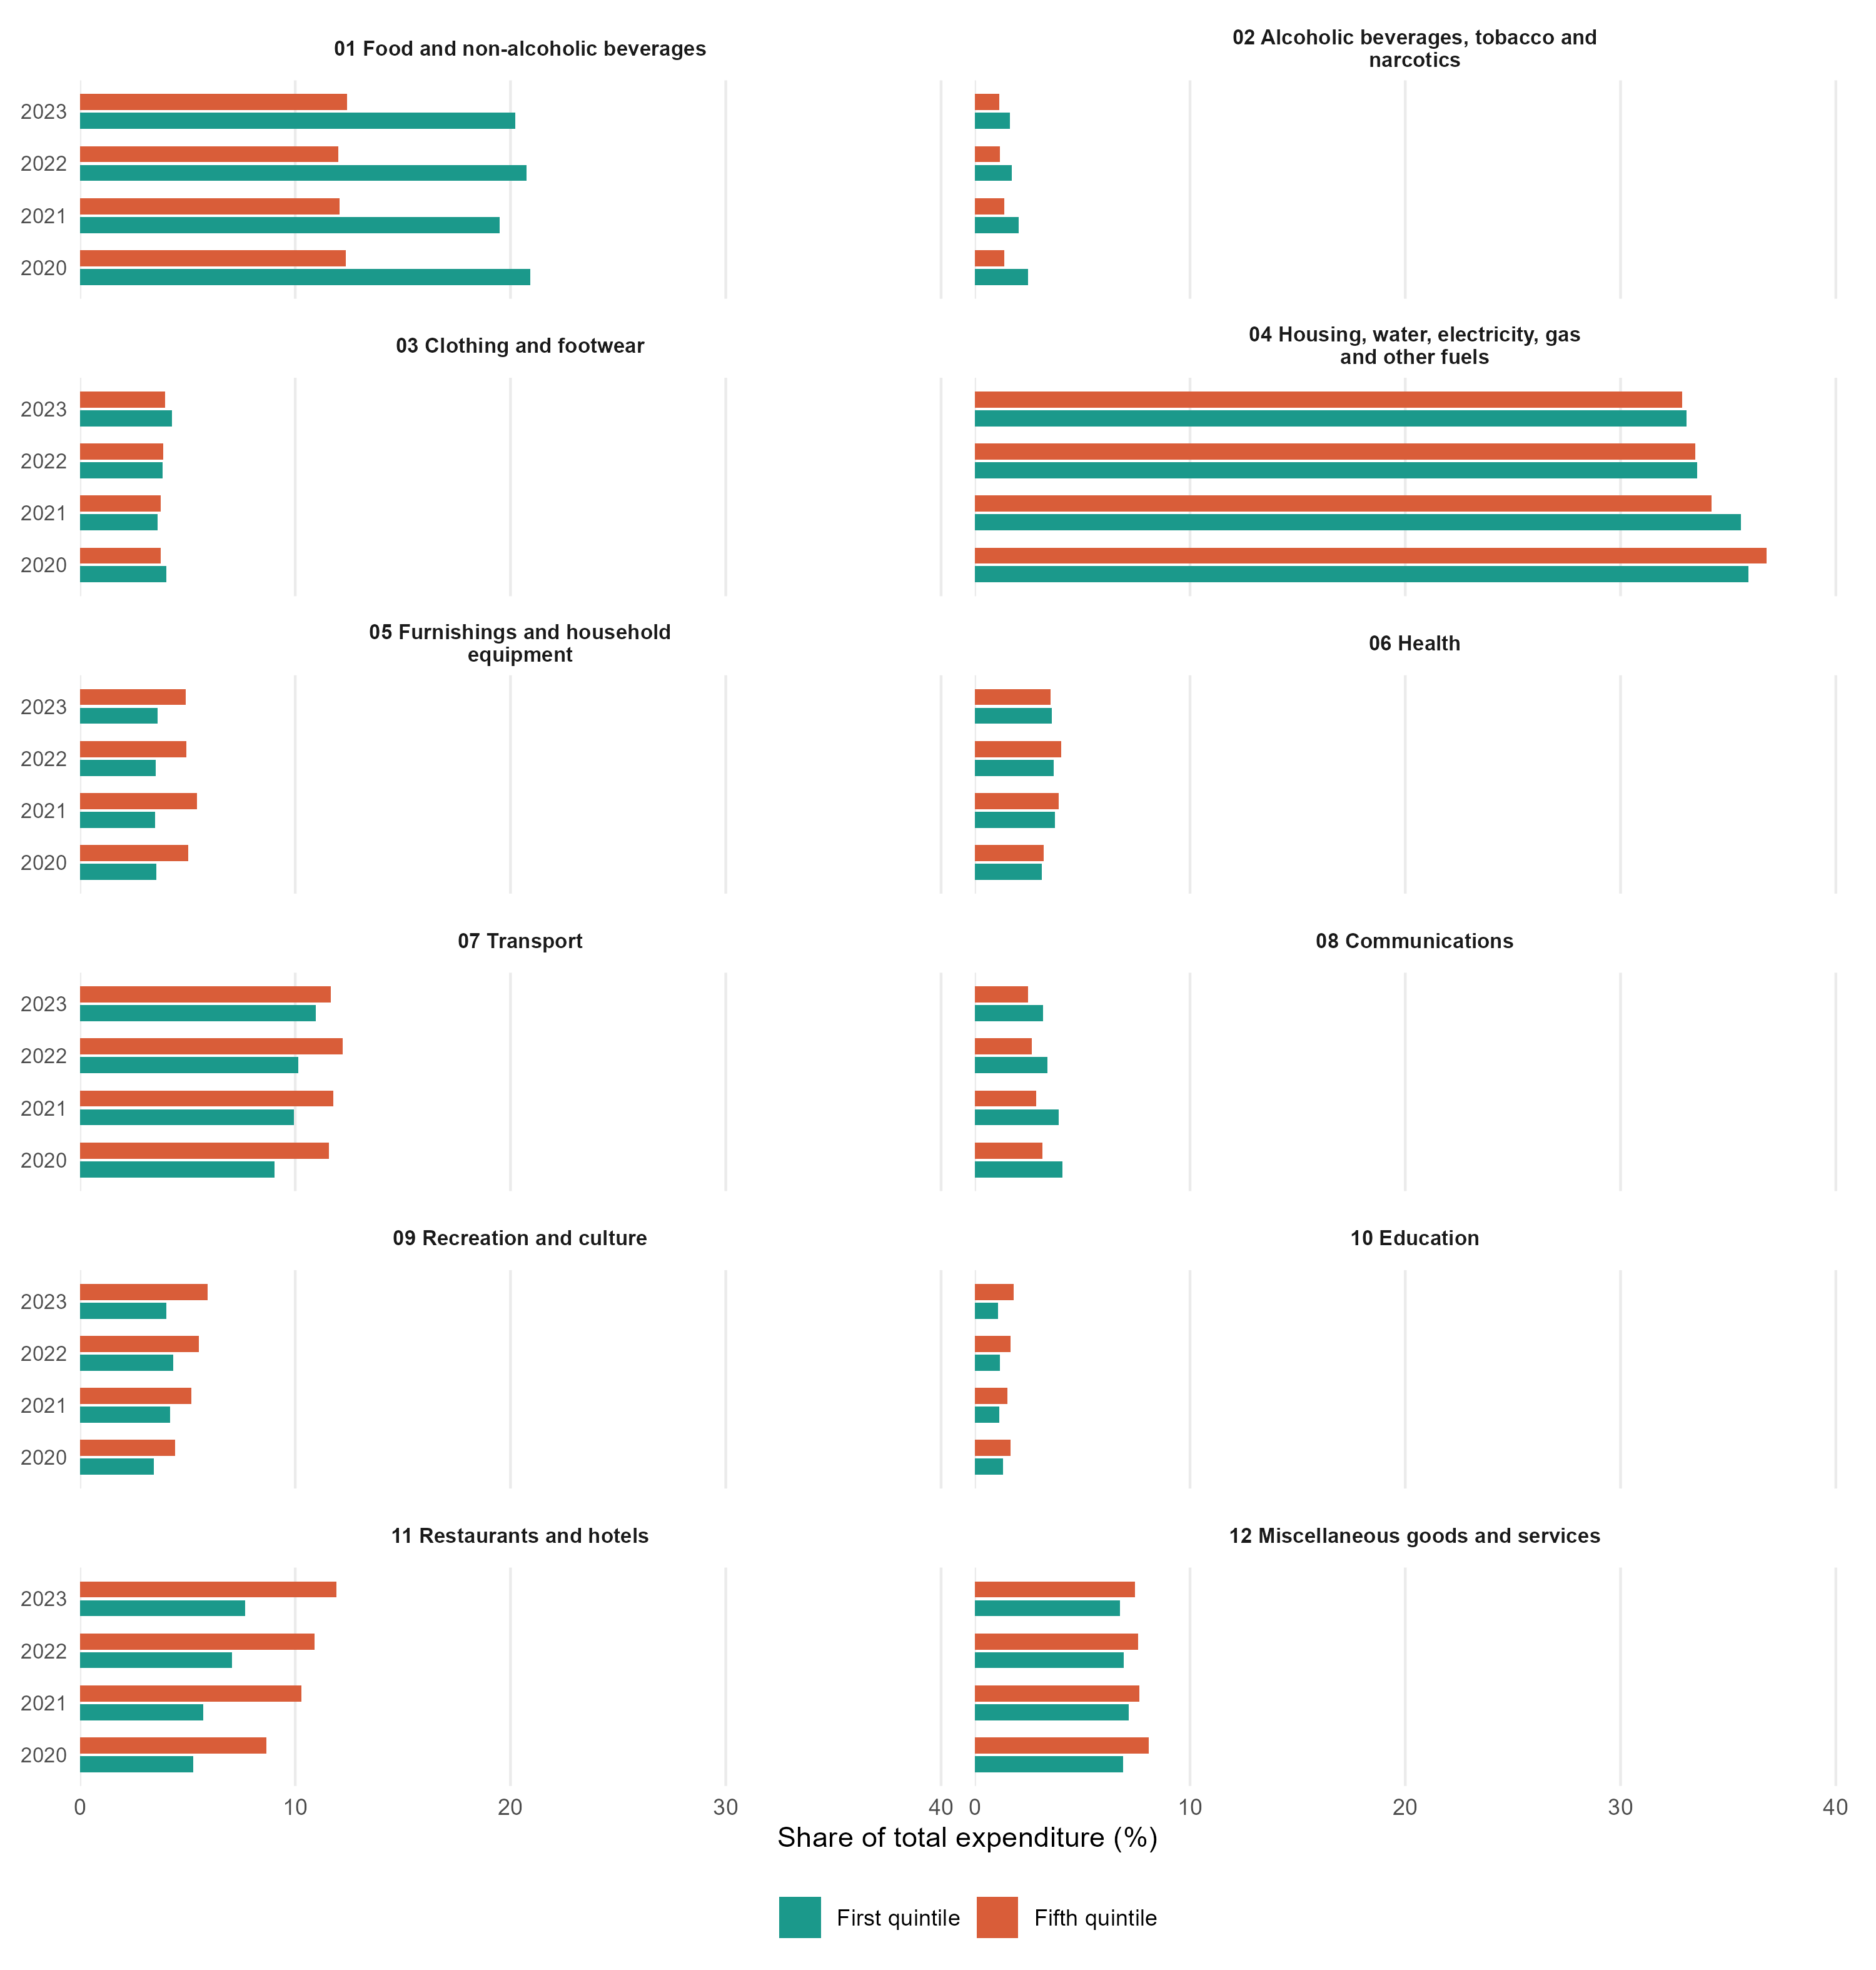
\includegraphics[width=0.98\textwidth,height=0.86\textheight,keepaspectratio]{fig/fig_ES_income_quintile_coicop_weights_2020_2023_grouped_bar.png}
\vspace{8pt}
\captionsetup{font=footnotesize, format=hang, singlelinecheck=false, justification=justified}
\caption*{Notes: The figure reports the share of each main COICOP category in total household expenditure for the first and fifth equivalized-income quintiles. Quintiles are computed separately by year using household weights.\\
Sources: INE Encuesta de Presupuestos Familiares public-use microdata; authors' calculations.}
\end{figure}
%%%%%%%%%%%%%%%%%%%%%%%%%%%%%%%%%%%%%%%%%%%%%%%%%%%%%%%%%%%%%%
\newpage



%%%%%%%%%%%%%%%%%%%%%%%%%%%%%%%%%%%%%%%%%%%%%%%%%%%%%%%%%%%%%%
\begin{figure}[H]
\centering
\caption{Essential and discretionary expenditures by income quintile, euro area (in \% of total expenditure)}
\label{fig:app-ea-essentials-discretionary}
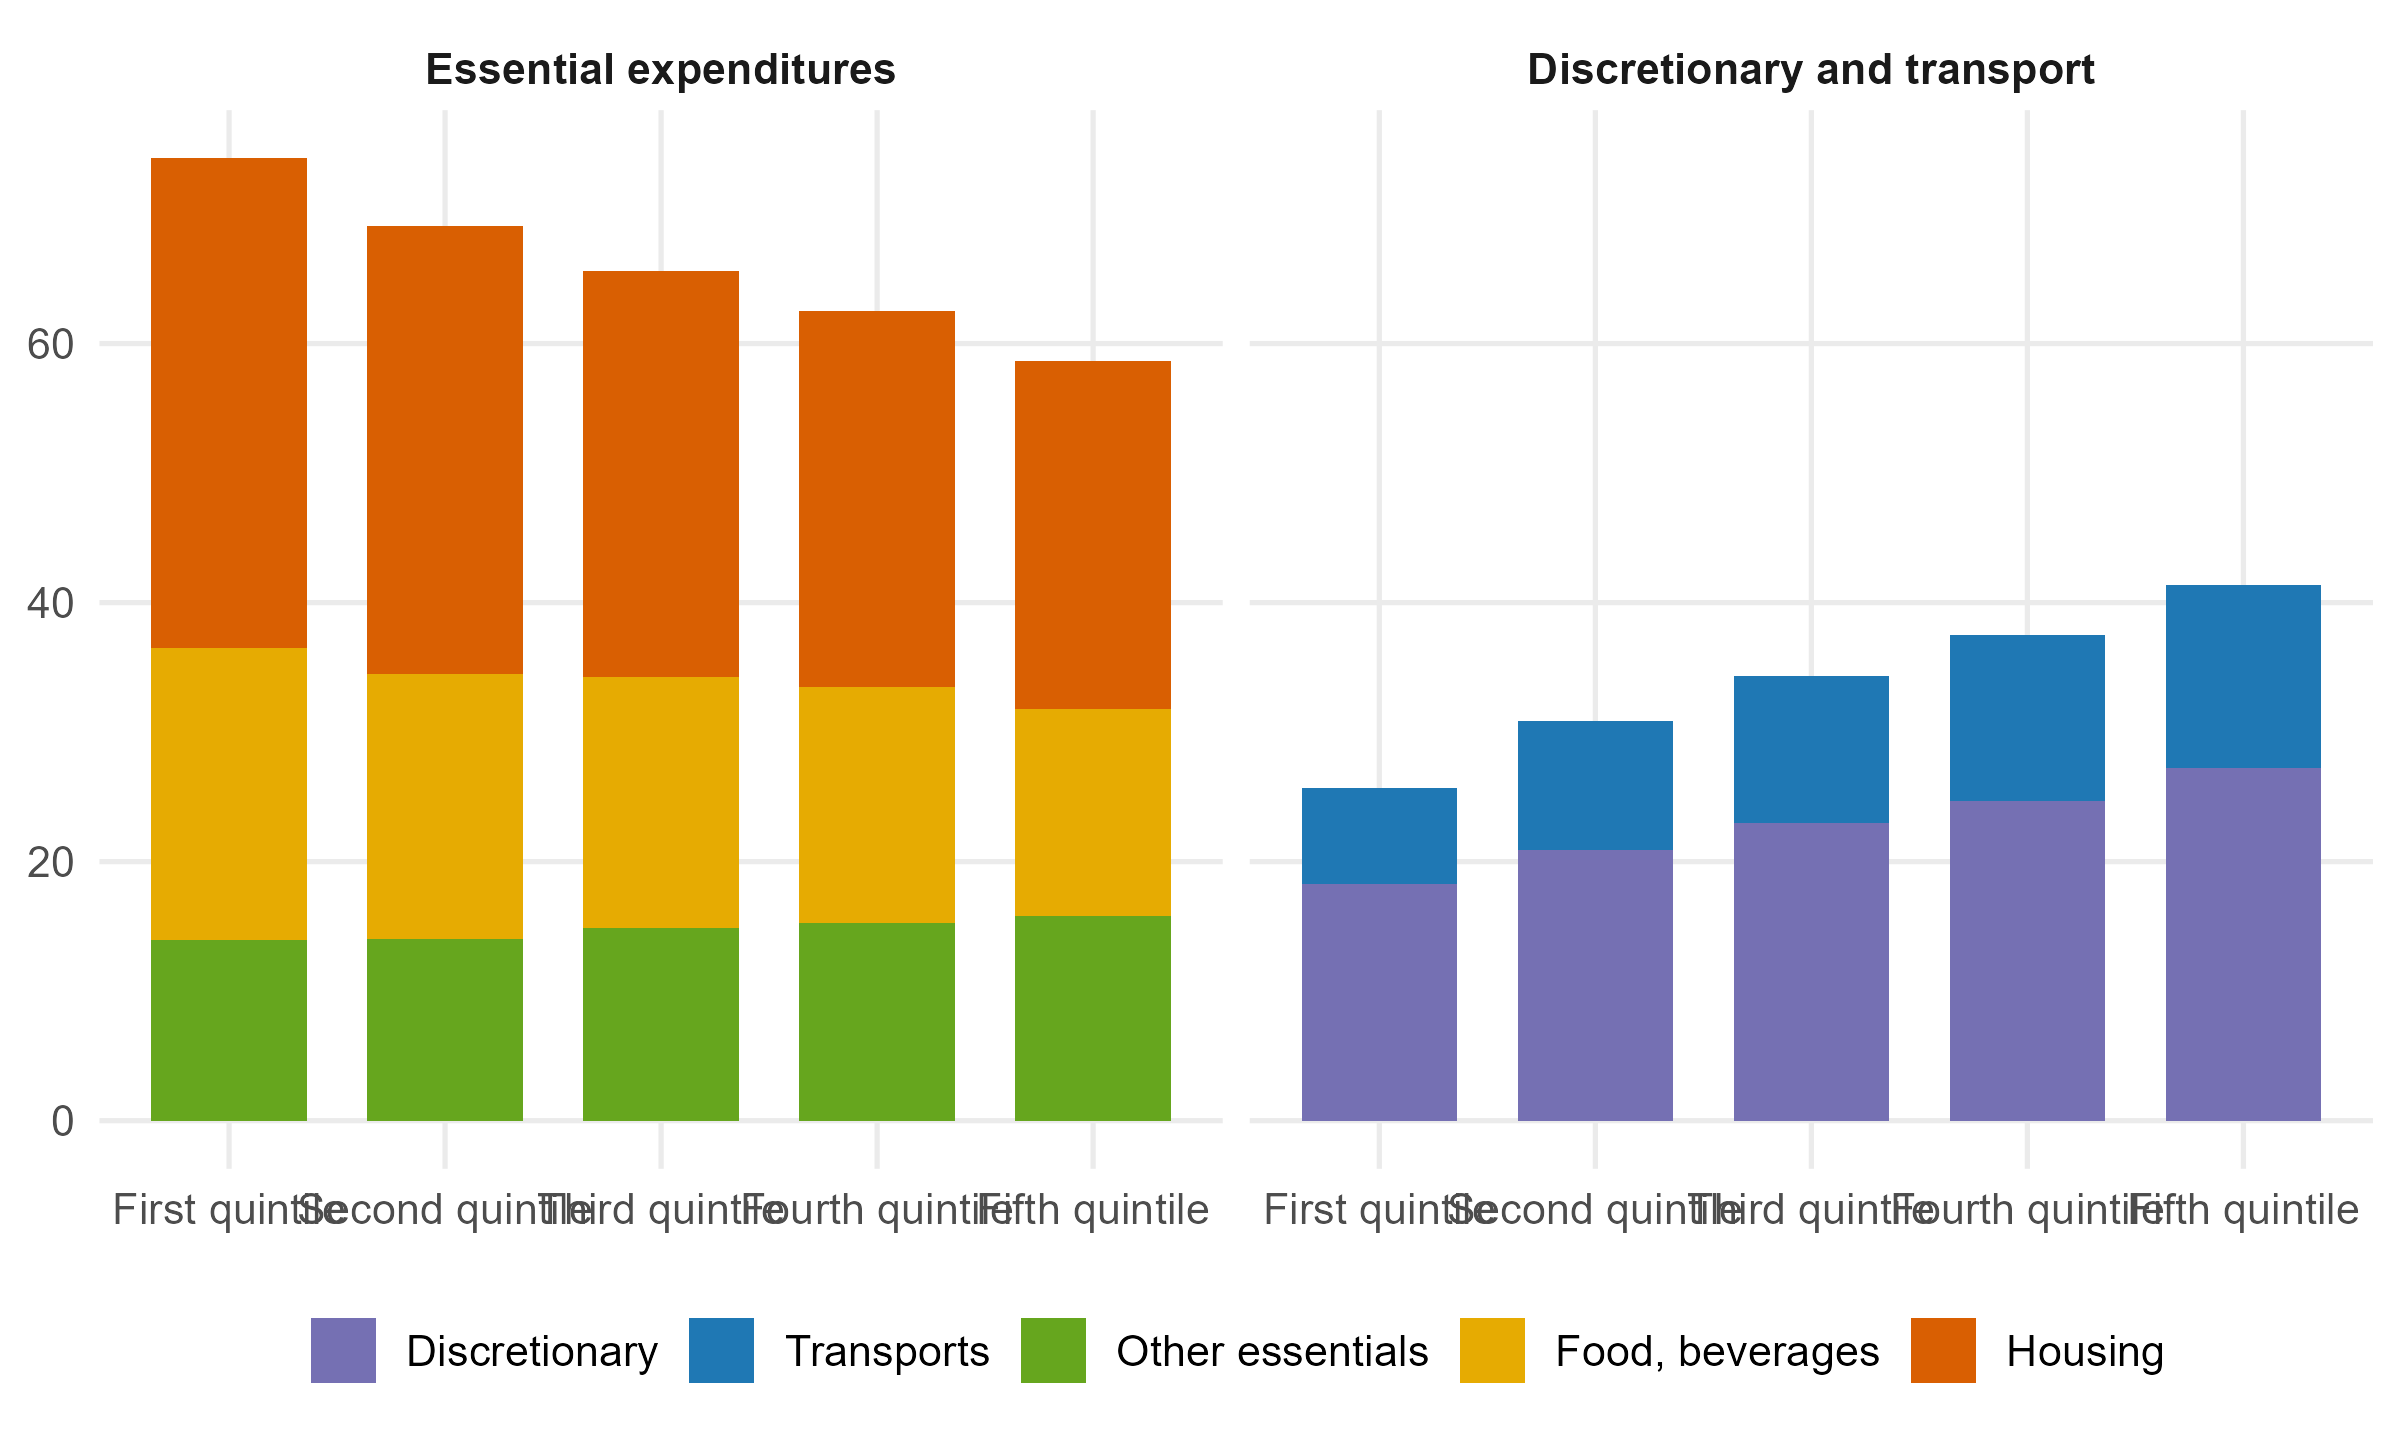
\includegraphics[width=0.96\textwidth,height=0.52\textheight,keepaspectratio]{fig/fig_EA_2015_income_essentials_discretionary_baskets.png}
\vspace{8pt}
\captionsetup{font=footnotesize, format=hang, singlelinecheck=false, justification=justified}
\caption*{Notes: The figure partitions COICOP expenditure shares into essential expenditures and discretionary/transport expenditures. The euro-area aggregate is computed as the unweighted average of available country-level HBS expenditure shares.\\
Sources: Eurostat HBS 2015; authors' calculations.}
\end{figure}
%%%%%%%%%%%%%%%%%%%%%%%%%%%%%%%%%%%%%%%%%%%%%%%%%%%%%%%%%%%%%%

\clearpage
% Auto-generated by scripts/07b_build_counterfactuals_appendix.R.
\clearpage
\begin{landscape}
\section{Counterfactuals}
\label{sec:app-counterfactuals}

This appendix reports country-level observed and counterfactual headline inflation series. Each figure aggregates all simulated energy and food price-policy layers available for the country, using the HICP item weights in the country CPI basket.

% Condensed from data/counterfactual_measure_assumptions.xlsx (include = TRUE).
\scriptsize
\setlength{\LTleft}{0pt}
\setlength{\LTright}{0pt}
\setlength{\tabcolsep}{2pt}
\renewcommand{\arraystretch}{1.08}
\captionof{table}{Price measures included in the national counterfactual simulations}
\label{tab:ea20-price-counterfactual-measures}
\vspace{0.3em}
\begin{longtable}{@{}p{0.72in}p{3.55in}p{1.05in}p{1.15in}p{1.75in}@{}}
\toprule
Country & Included price measures & COICOP components & Assumption window & Instrument classification \\
\midrule
\endfirsthead
\toprule
Country & Included price measures & COICOP components & Assumption window & Instrument classification \\
\midrule
\endhead
\midrule
\multicolumn{5}{r}{\emph{Continued on next page}}\\
\endfoot
\bottomrule
\endlastfoot
Austria & Electricity price brake; electricity and gas excise cuts & CP0451, CP0452 & 2022-05-01--2024-12-01 & Administered: 2; other calibrated: 2. \\
Belgium & Social energy tariffs; household energy VAT cuts; fuel-excise cut & CP0451, CP0452, CP0722 & 2022-03-01--2023-12-01 & VAT/excise: 2; administered: 1; fuel: 1; other calibrated: 2. \\
Croatia & Heating and electricity price support; gas and food VAT cuts & CP0112, CP0113, CP0114, CP0115, CP0116, CP0117, CP0451, CP0452, CP0455 & 2022-04-01--2023-12-01 & VAT/excise: 7; administered: 2. \\
Cyprus & Electricity VAT cuts and bill subsidy; heating- and transport-fuel excise cuts & CP0451, CP0453, CP0722 & 2021-11-01--2023-02-01 & VAT/excise: 2; fuel: 1; other calibrated: 2. \\
Estonia & Energy network-fee rebates; heating, electricity, and gas compensation; fuel- and electricity-excise deferrals; regulated electricity service & CP0451, CP0452, CP0455, CP0722 & 2021-10-01--2024-03-01 & Administered: 4; fuel: 1; other calibrated: 3. \\
Finland & Biofuel-obligation cut; electricity and passenger-transport VAT cuts & CP0451, CP0722, CP0731, CP0732, CP0733, CP0734 & 2022-05-01--2023-12-01 & VAT/excise: 5; fuel: 1. \\
France & Gas and electricity tariff shields; energy-tax cuts; transport-fuel rebates & CP0451, CP0452, CP0722 & 2021-11-01--2023-12-01 & Administered: 2; fuel: 1. \\
Germany & Electricity-levy abolition; electricity and gas price brakes; gas VAT and transport-fuel tax cuts & CP0451, CP0452, CP0722 & 2022-06-01--2024-03-01 & VAT/excise: 1; administered: 2; fuel: 1; other calibrated: 1. \\
Greece & Household electricity and gas subsidies; diesel subsidy & CP0451, CP0452, CP0722 & 2021-09-01--2023-12-01 & Administered: 2; fuel: 1. \\
Ireland & Electricity credits and levy reduction; household energy VAT cuts; transport-fuel excise cuts & CP0451, CP0452, CP0722 & 2022-03-01--2023-09-01 & VAT/excise: 2; fuel: 1; other calibrated: 2. \\
Italy & Electricity and gas charge reductions; social energy bonuses; gas VAT and transport-fuel excise cuts & CP0451, CP0452, CP0722 & 2021-10-01--2023-12-01 & VAT/excise: 1; administered: 2; fuel: 1; other calibrated: 2. \\
Latvia & Heating- and fuel-price compensation; electricity charge reductions & CP0451, CP0452, CP0454, CP0455, CP0722 & 2022-01-01--2023-04-01 & Administered: 1; fuel: 1; other calibrated: 3. \\
Lithuania & Household electricity and gas subsidies & CP0451, CP0452 & 2022-07-01--2023-06-01 & Administered: 2. \\
Luxembourg & Electricity and gas price support; broad temporary VAT cuts; transport-fuel rebate & Numerous COICOP & 2022-02-01--2024-12-01 & VAT/excise: 67; administered: 3; fuel: 1; other calibrated: 1. \\
Malta & Household electricity and transport-fuel price subsidies & CP0451, CP0722 & 2022-01-01--2023-12-01 & Administered: 2. \\
Netherlands & Electricity and gas price caps; energy VAT and tax relief; transport-fuel excise cuts & CP0451, CP0452, CP0722 & 2022-01-01--2023-12-01 & VAT/excise: 2; administered: 2; fuel: 2; other calibrated: 2. \\
Portugal & Zero-VAT food basket; electricity and gas price measures; electricity-network support; transport-fuel tax cuts & CP0111, CP0112, CP0113, CP0114, CP0115, CP0116, CP0117, CP0122, CP0451, CP0452, CP0722 & 2021-09-01--2026-04-01 & VAT/excise: 9; administered: 2; fuel: 1; other calibrated: 1. \\
Slovakia & Household electricity, gas, and heating price caps & CP0451, CP0452, CP0455 & 2023-01-01--2023-12-01 & Administered: 3. \\
Slovenia & Household energy price caps; excise and network-charge reductions; regulated transport-fuel prices & CP0451, CP0452, CP0453, CP0455, CP0722 & 2021-11-01--2023-12-01 & Administered: 5; other calibrated: 5. \\
Spain & Food and household-energy VAT cuts; electricity tax cuts; electricity and gas price measures; transport-fuel rebate & CP0111, CP0114, CP0115, CP0116, CP0117, CP0451, CP0452, CP0722 & 2021-06-01--2026-04-01 & VAT/excise: 8; administered: 4; fuel: 1; other calibrated: 2. \\
\end{longtable}
\par\vspace{0.35em}\footnotesize\noindent Notes: The table summarizes the modelled price measures underlying Table~\ref{tab:ea20-policy-category-contributions}. The last column applies the same mutually exclusive instrument classification as Table~\ref{tab:ea20-policy-category-contributions}; counts sum to the number of included measures for each country. ``Other calibrated'' contains measures that cannot be assigned to the VAT/excise, administered-price, or fuel-support families. The adjacent column reports the affected COICOP components. Transport-fuel measures are assigned only to fuels and lubricants, not to the broader vehicle-operation group used in the product decompositions. Sources: Bruegel Dataset (2021), `National policies to shield consumers from rising energy prices,' version of 26 June 2023; national sources; authors' calculations.

\end{landscape}
\clearpage

\subsection{Austria}
\begin{figure}[H]
\centering
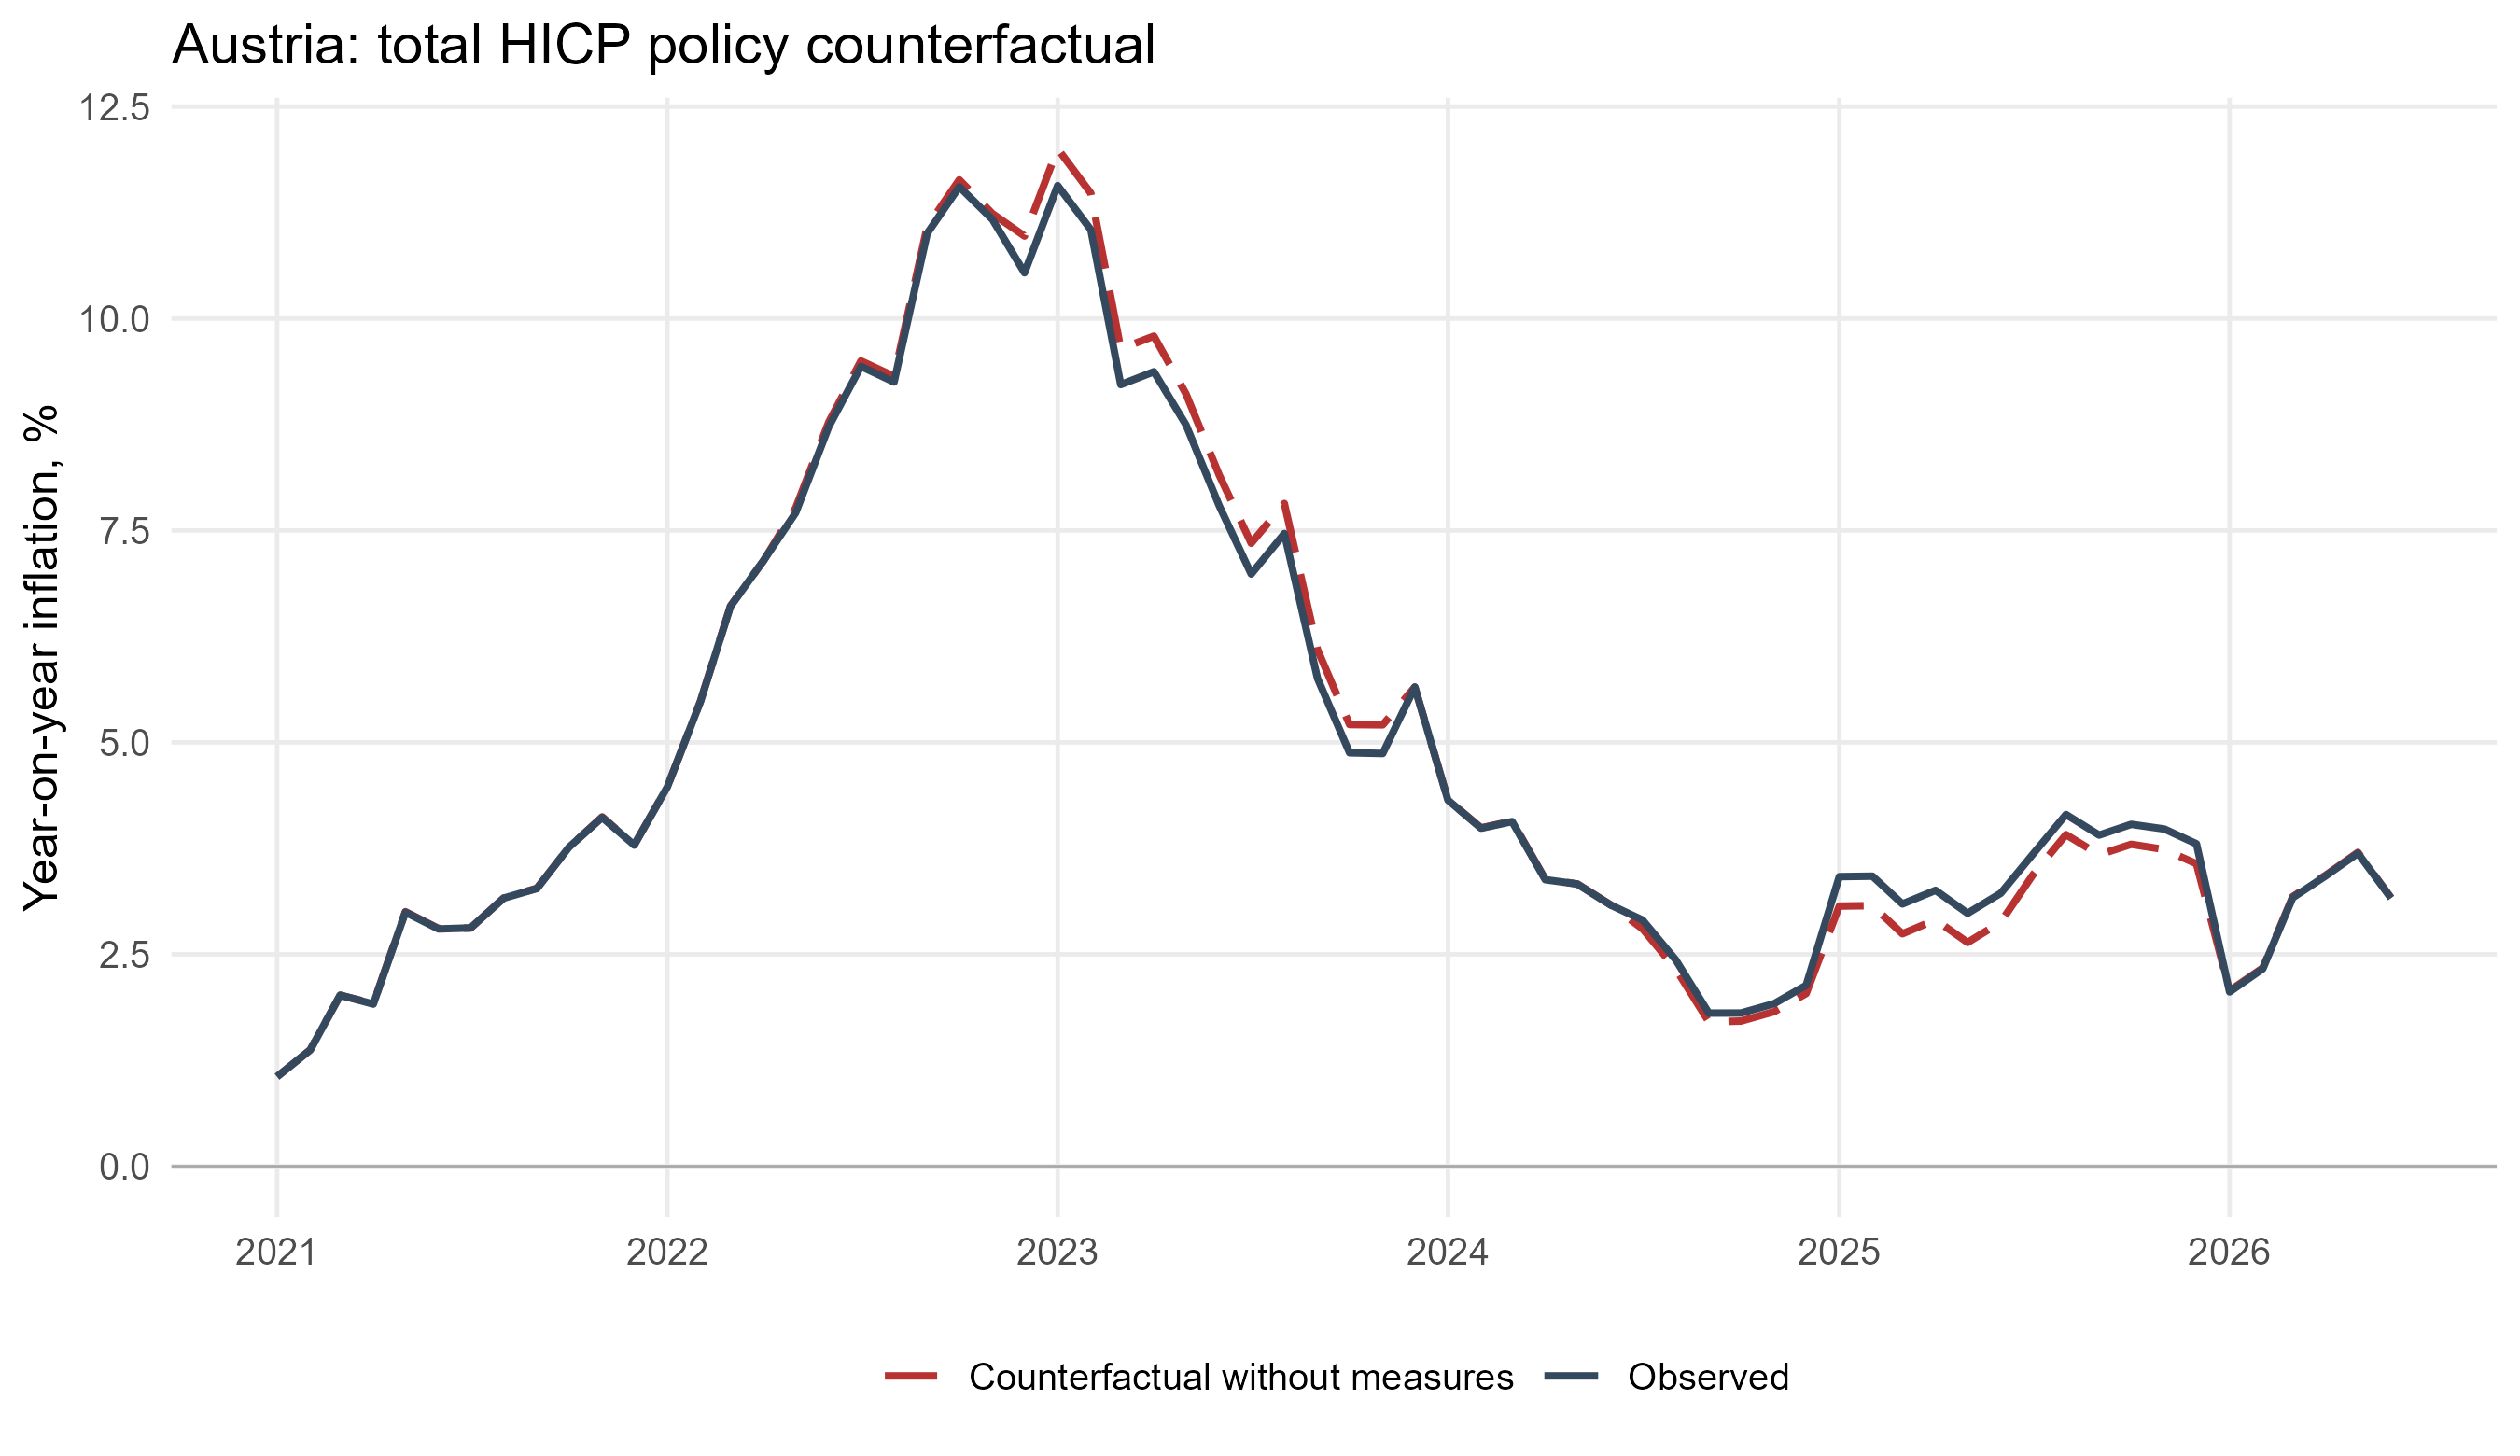
\includegraphics[width=0.86\textwidth,height=0.38\textheight,keepaspectratio]{fig/policy_total_cpi_counterfactual_inflation_AT_austria.png}
\caption{Austria: observed and counterfactual inflation}
\end{figure}

\subsection{Belgium}
\begin{figure}[H]
\centering
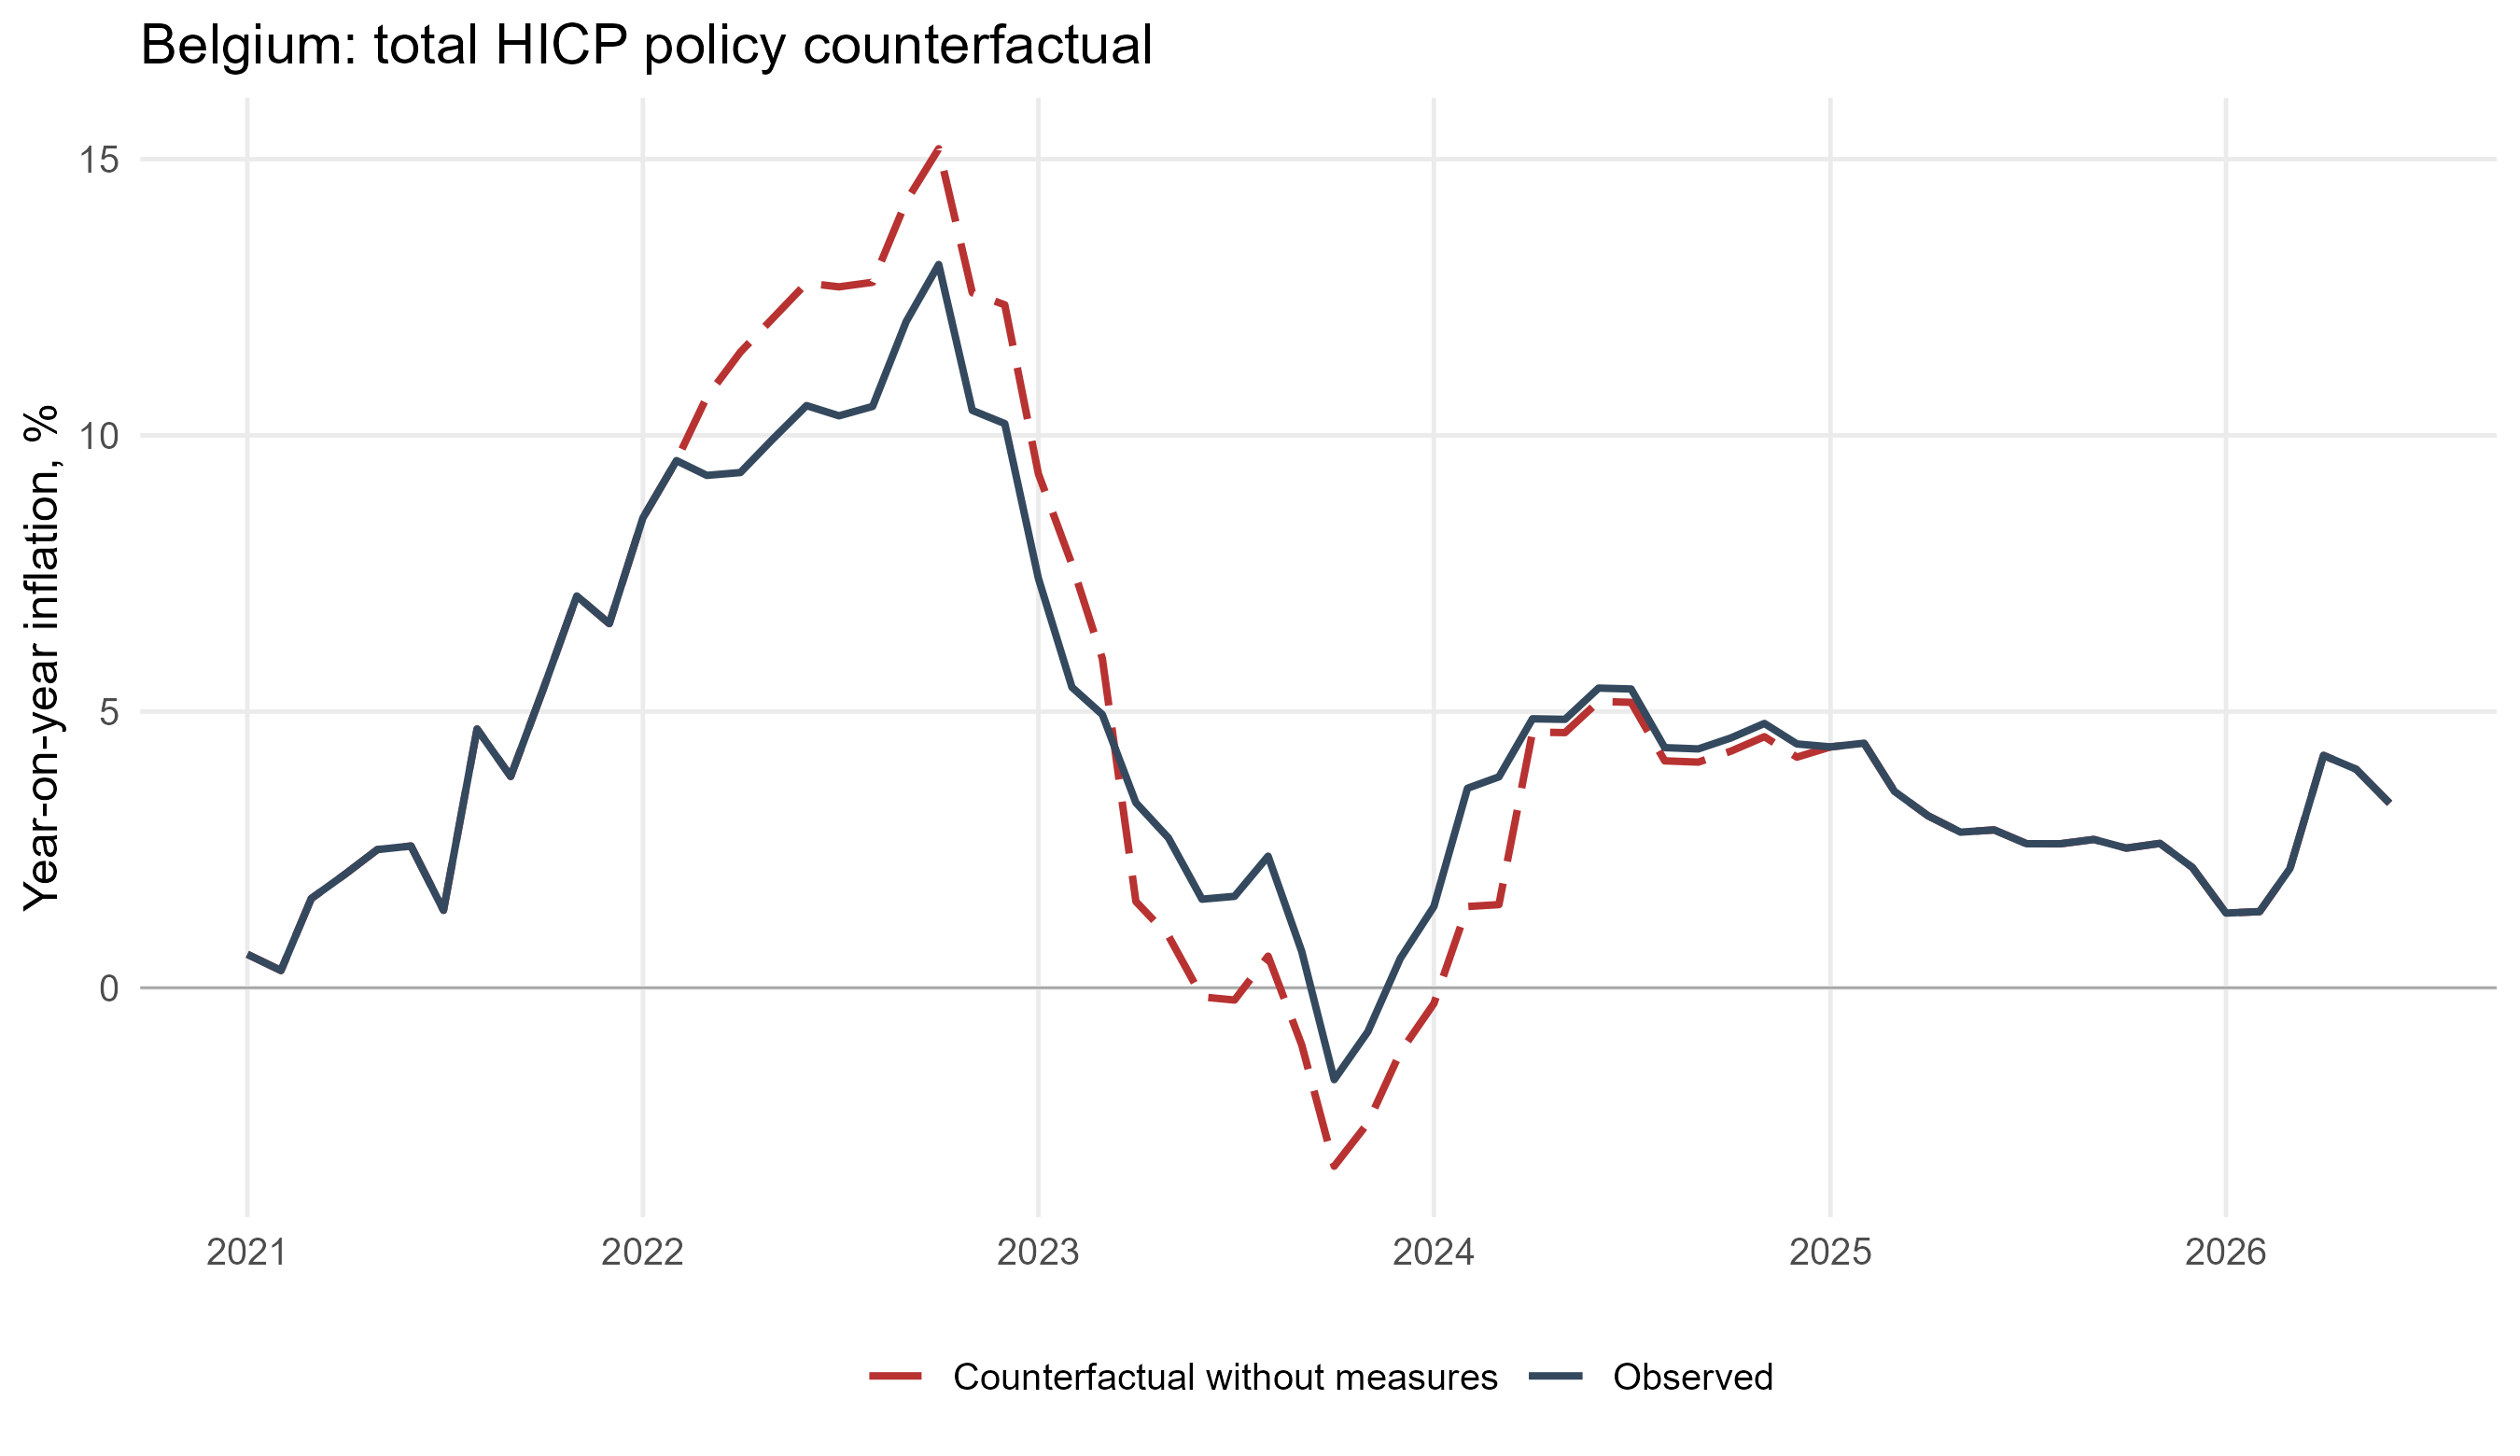
\includegraphics[width=0.86\textwidth,height=0.38\textheight,keepaspectratio]{fig/policy_total_cpi_counterfactual_inflation_BE_belgium.png}
\caption{Belgium: observed and counterfactual inflation}
\end{figure}

\subsection{Cyprus}
\begin{figure}[H]
\centering
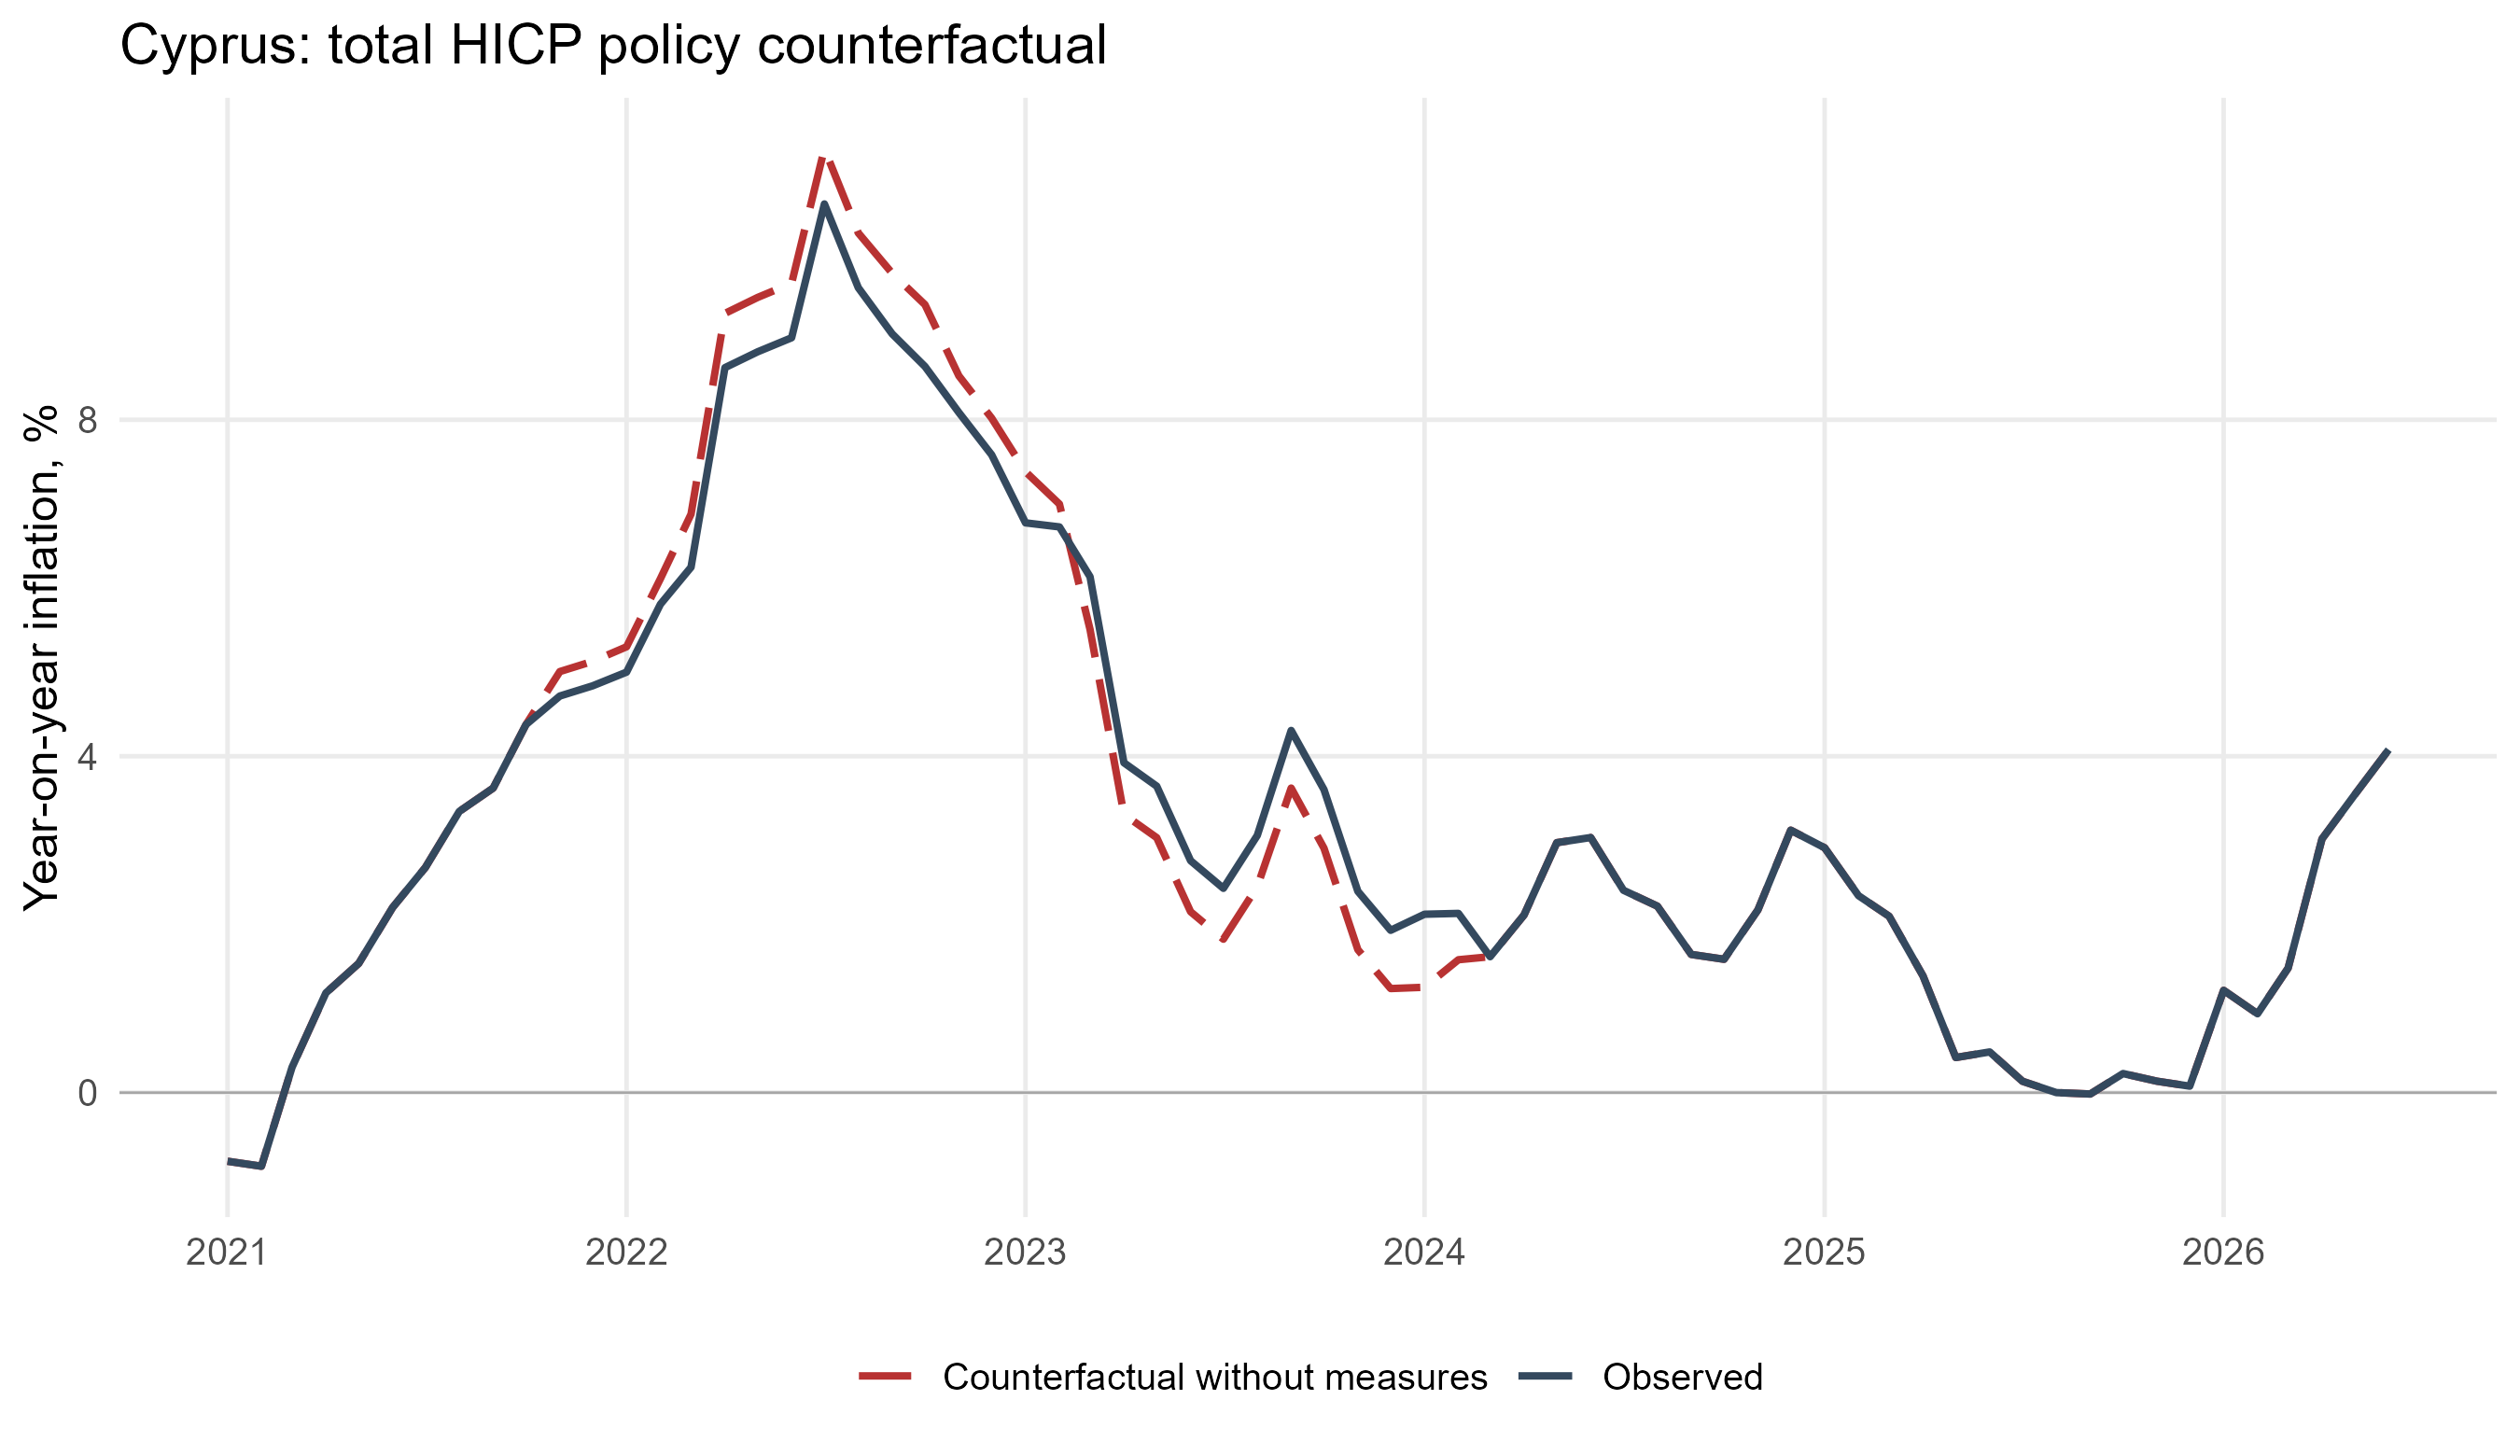
\includegraphics[width=0.86\textwidth,height=0.38\textheight,keepaspectratio]{fig/policy_total_cpi_counterfactual_inflation_CY_cyprus.png}
\caption{Cyprus: observed and counterfactual inflation}
\end{figure}

\subsection{Germany}
\begin{figure}[H]
\centering
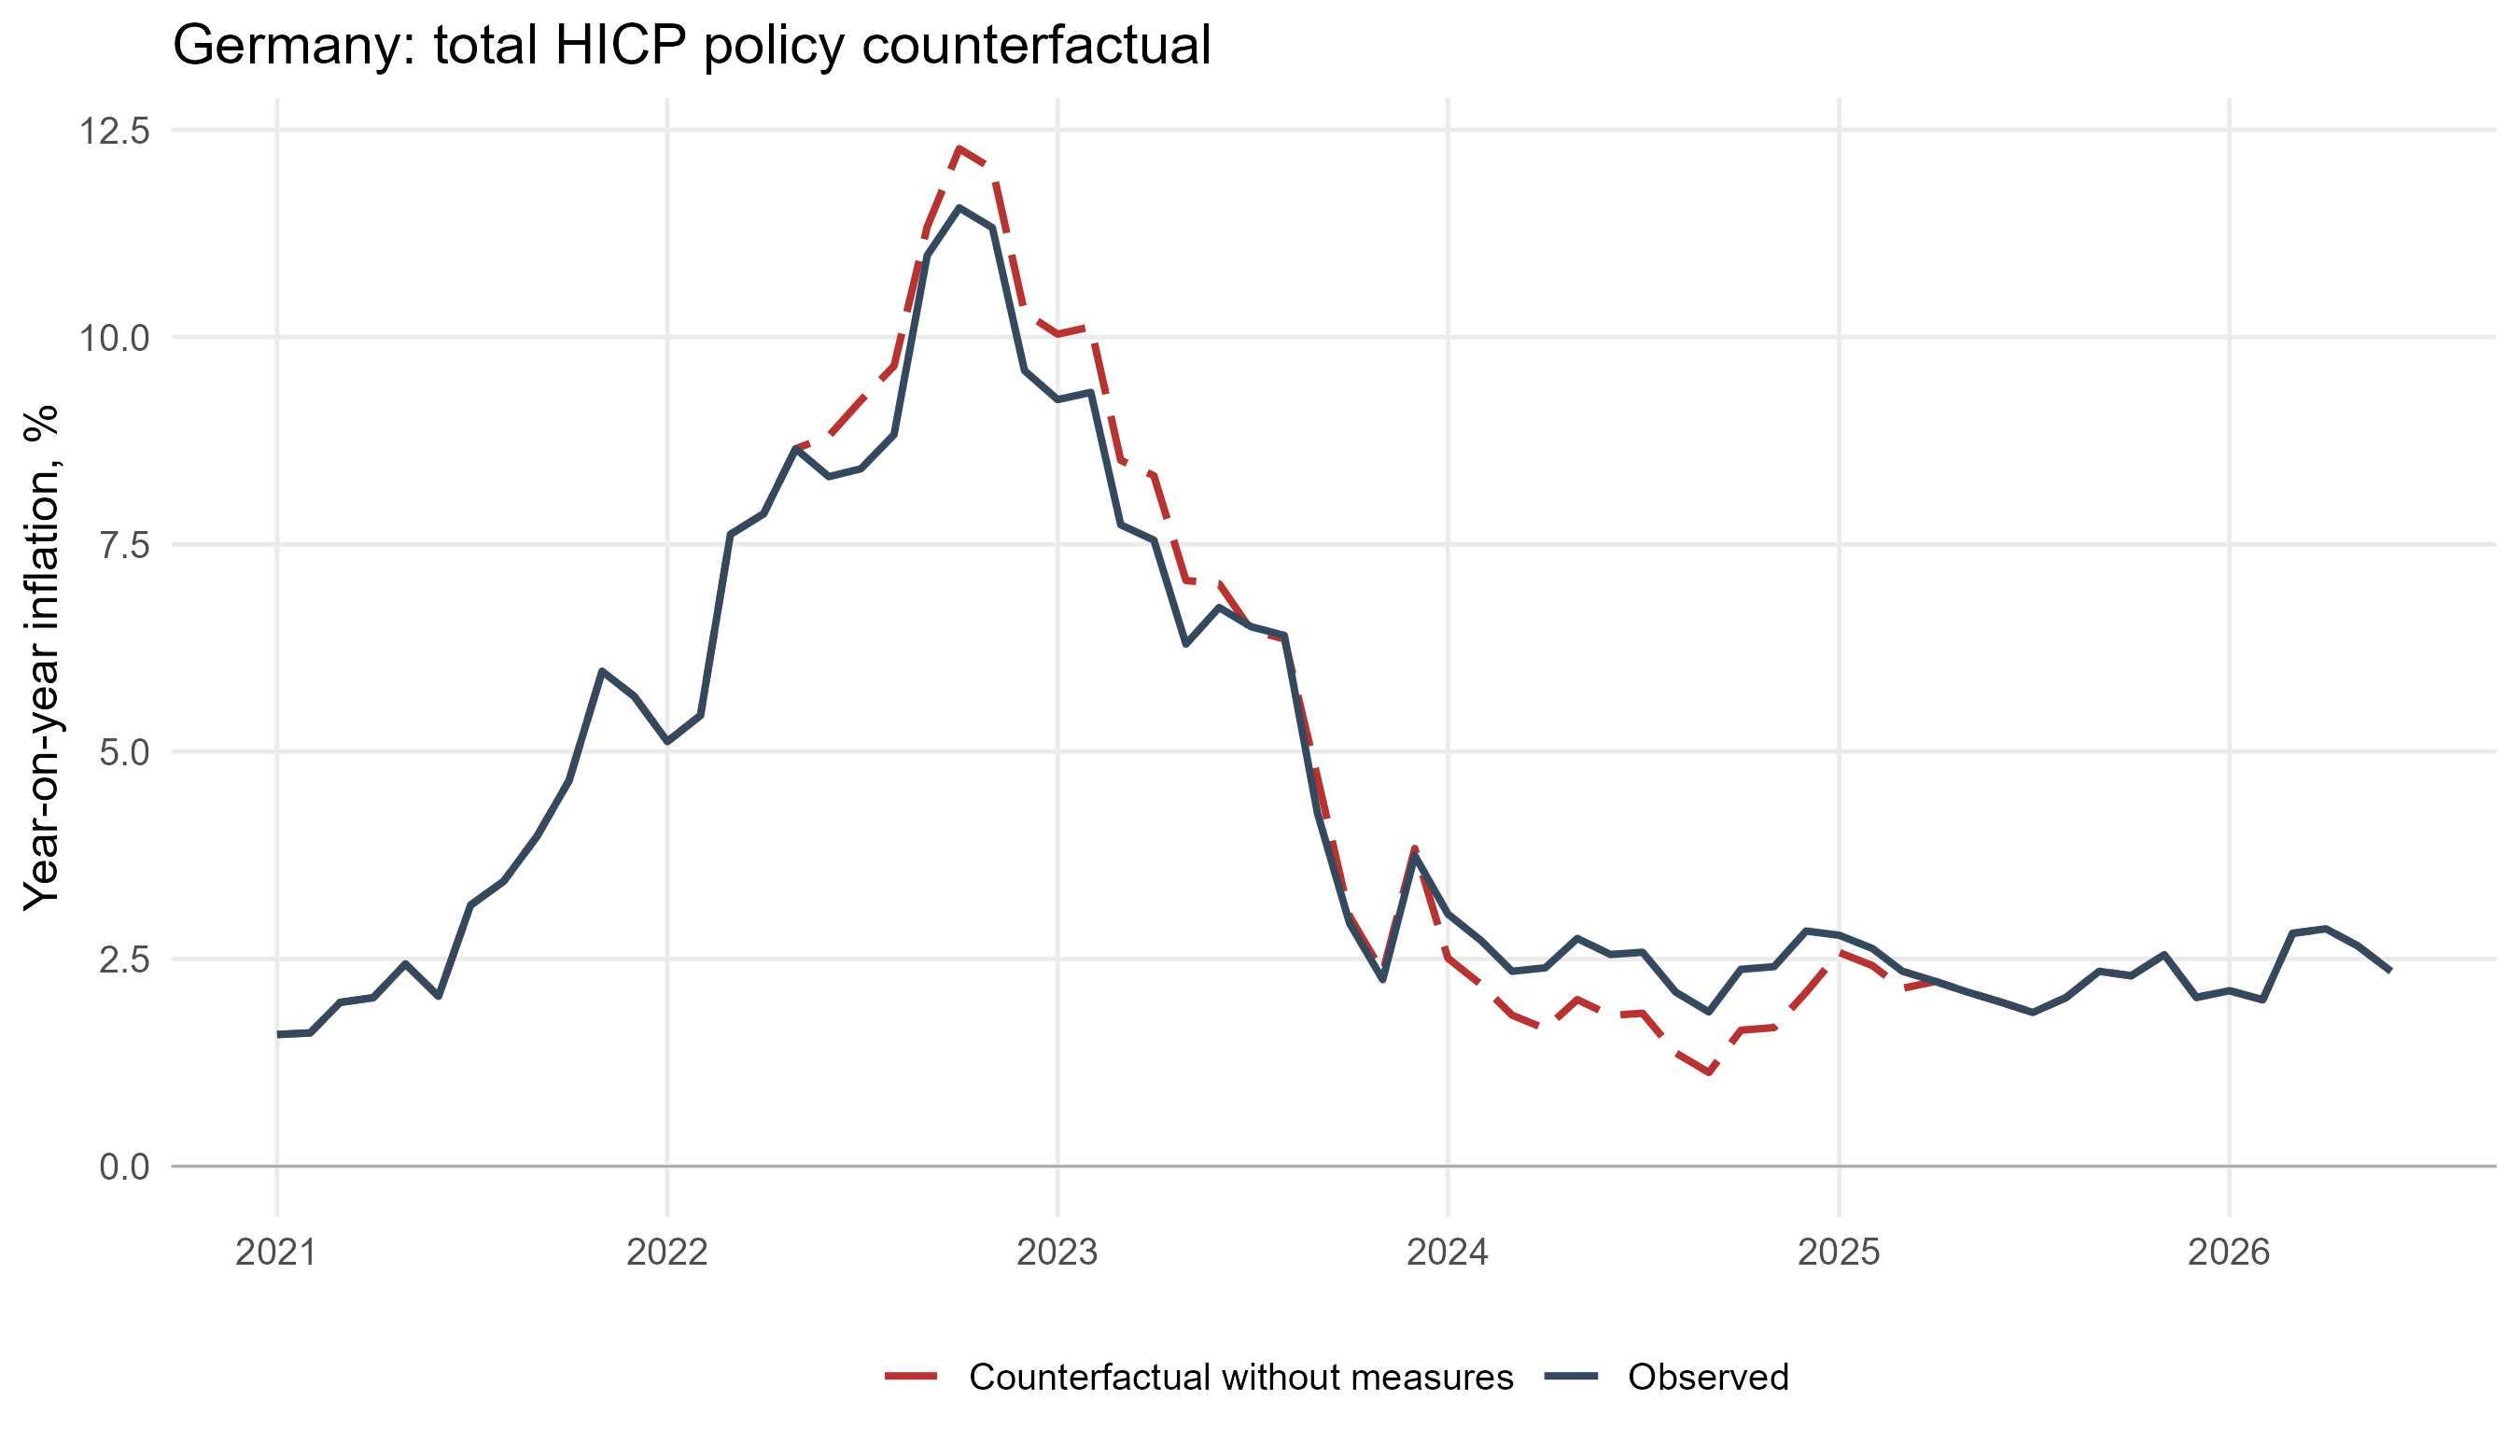
\includegraphics[width=0.86\textwidth,height=0.38\textheight,keepaspectratio]{fig/policy_total_cpi_counterfactual_inflation_DE_germany.png}
\caption{Germany: observed and counterfactual inflation}
\end{figure}

\subsection{Estonia}
\begin{figure}[H]
\centering
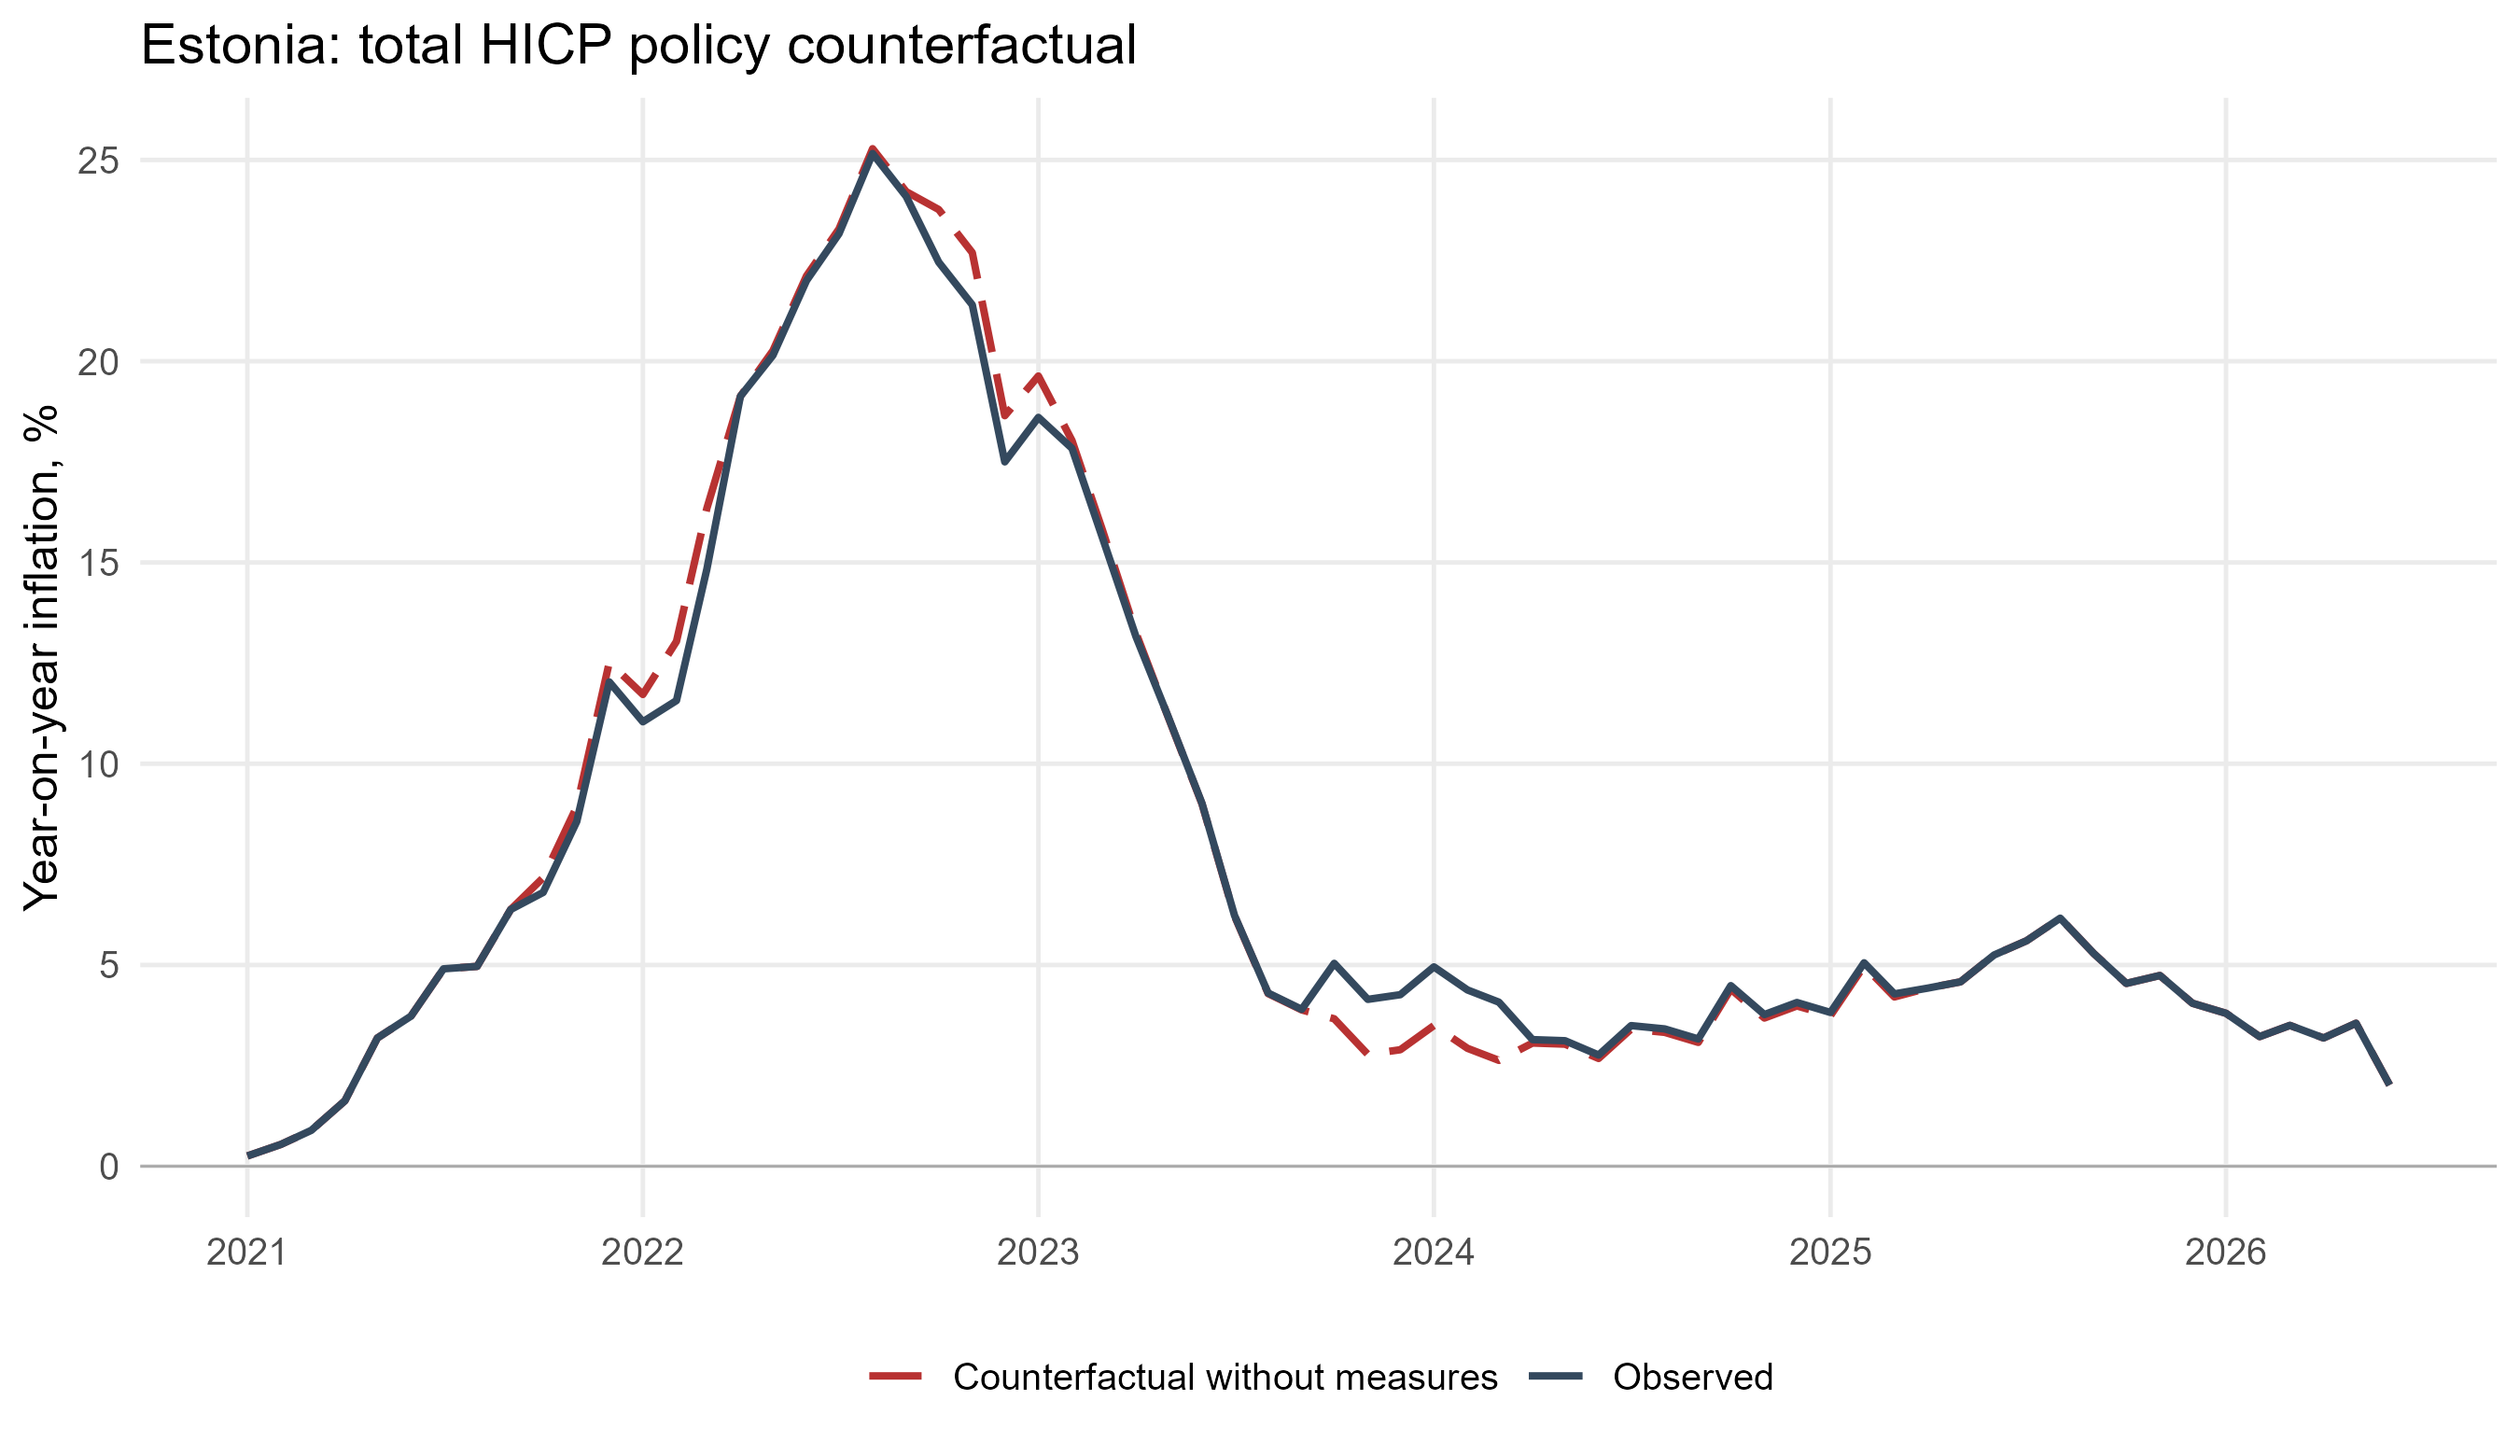
\includegraphics[width=0.86\textwidth,height=0.38\textheight,keepaspectratio]{fig/policy_total_cpi_counterfactual_inflation_EE_estonia.png}
\caption{Estonia: observed and counterfactual inflation}
\end{figure}

\subsection{Greece}
\begin{figure}[H]
\centering
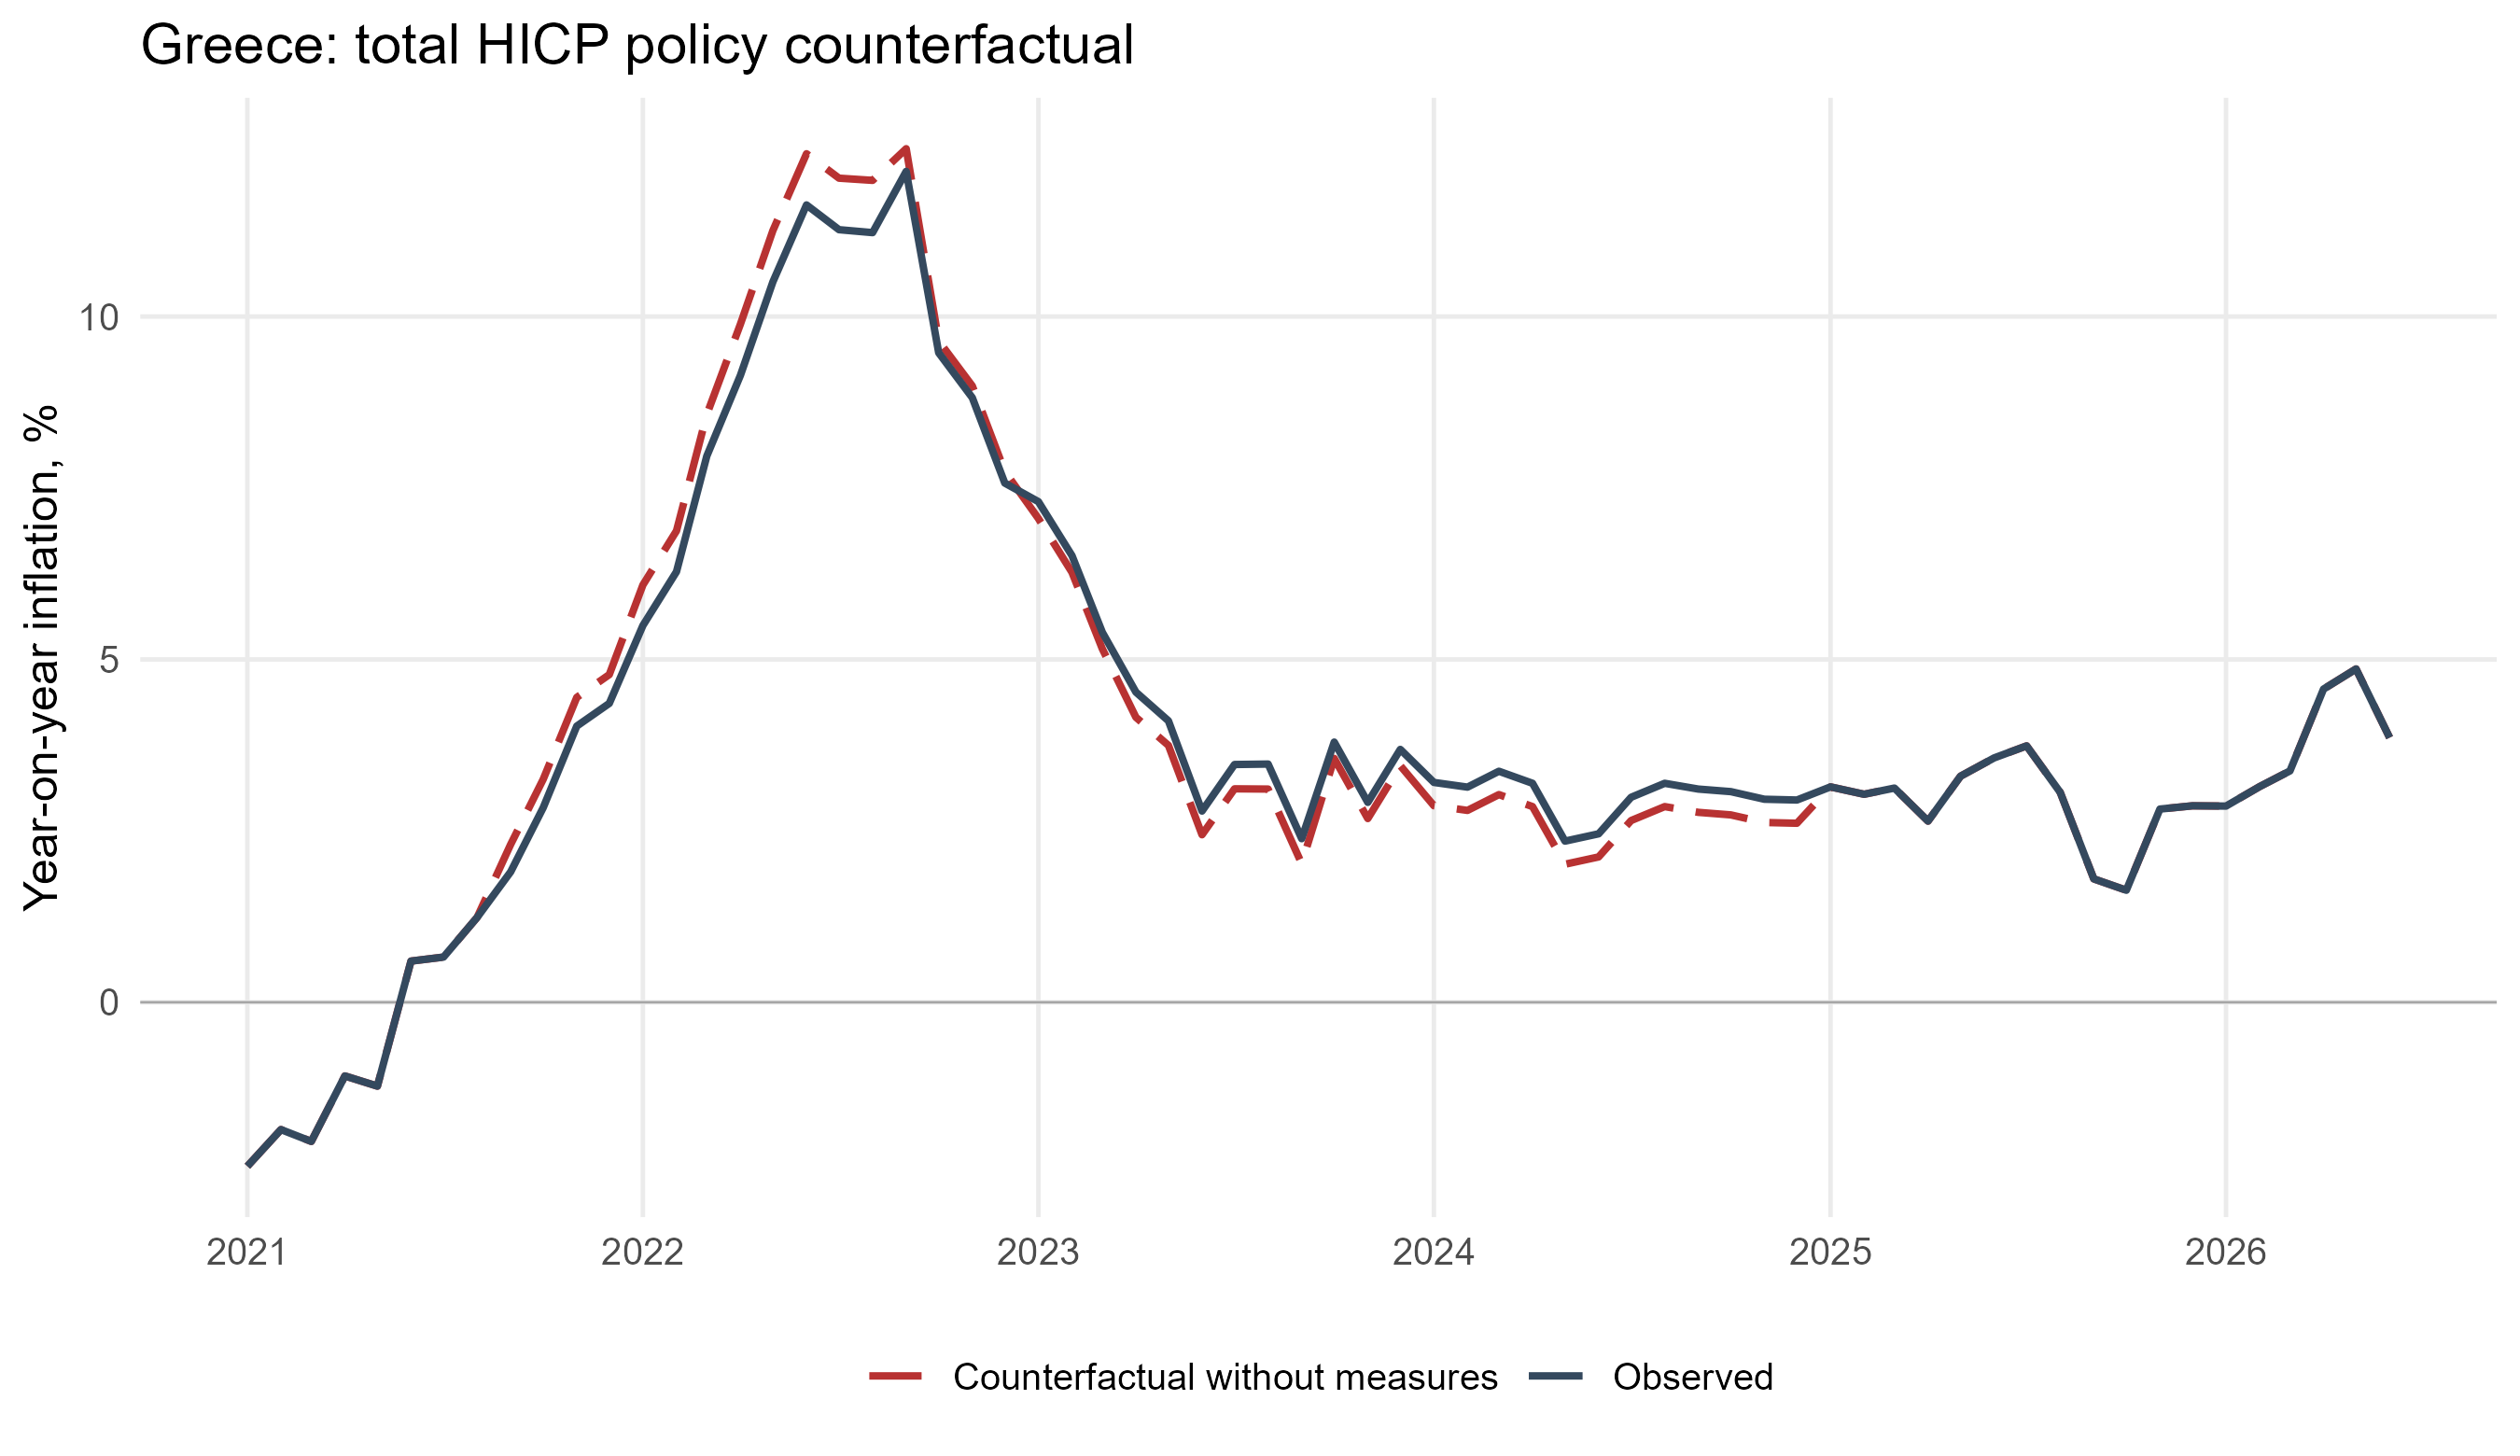
\includegraphics[width=0.86\textwidth,height=0.38\textheight,keepaspectratio]{fig/policy_total_cpi_counterfactual_inflation_EL_greece.png}
\caption{Greece: observed and counterfactual inflation}
\end{figure}

\subsection{Spain}
\begin{figure}[H]
\centering
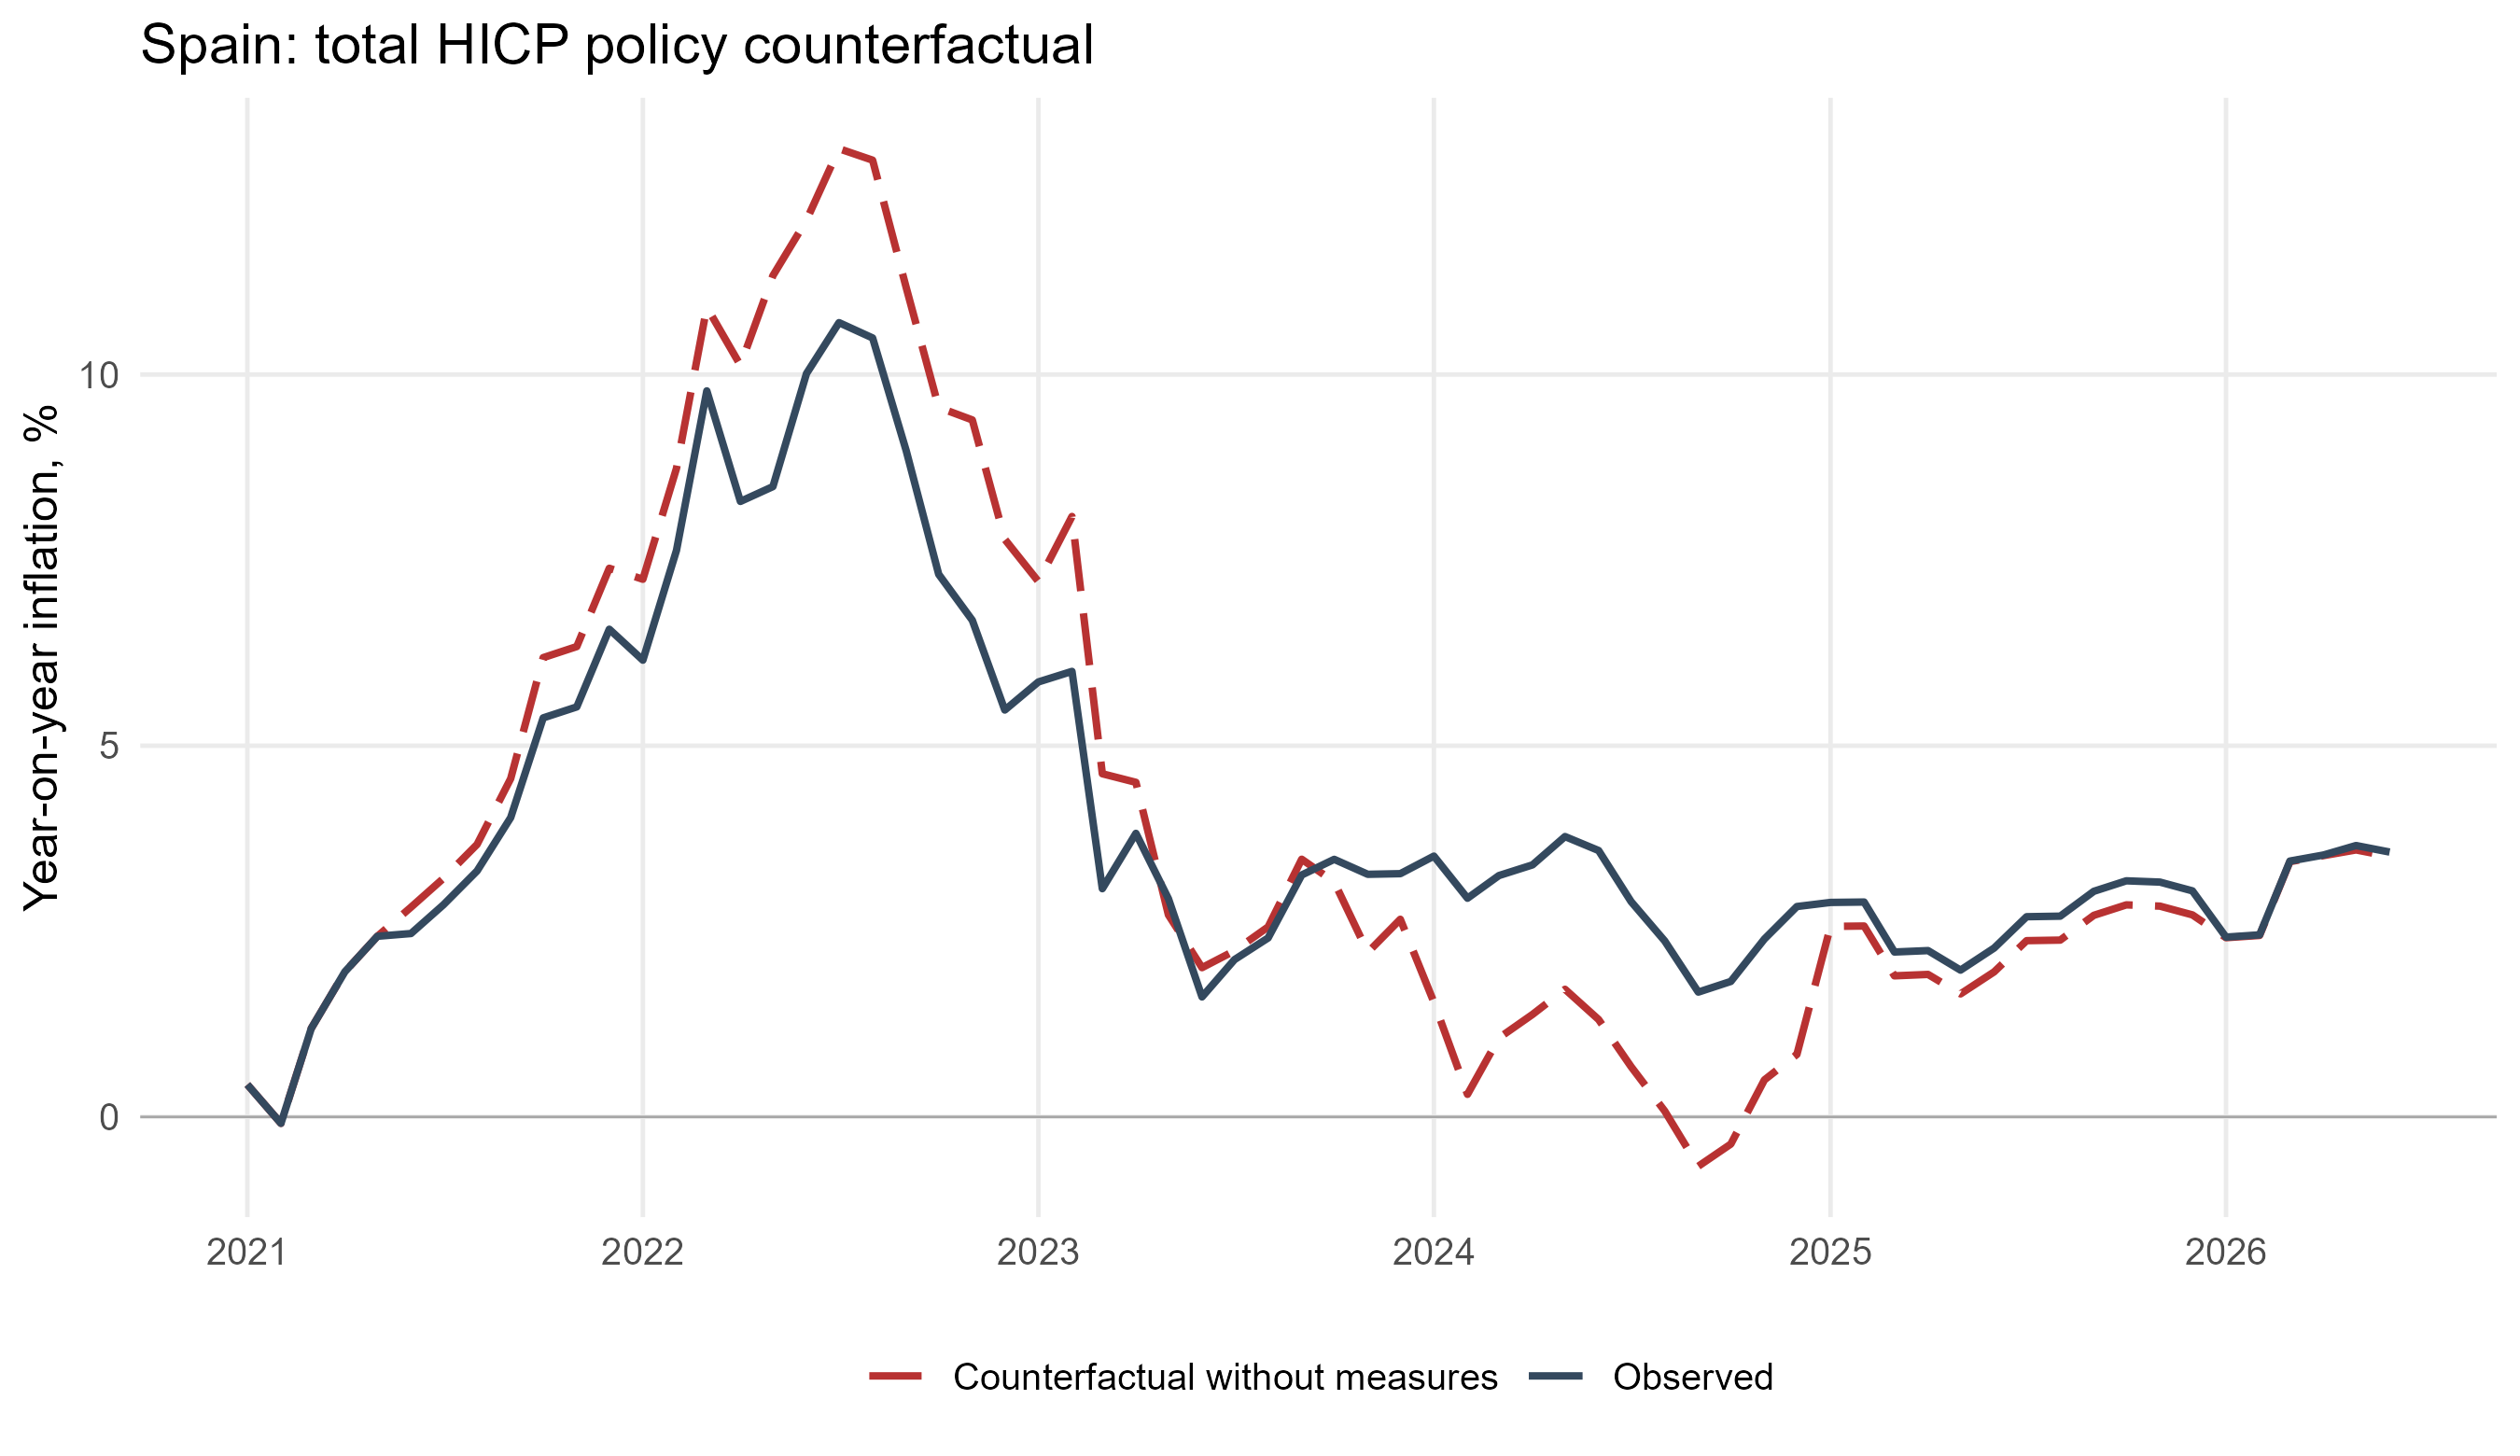
\includegraphics[width=0.86\textwidth,height=0.38\textheight,keepaspectratio]{fig/policy_total_cpi_counterfactual_inflation_ES_spain.png}
\caption{Spain: observed and counterfactual inflation}
\end{figure}

\subsection{Finland}
\begin{figure}[H]
\centering
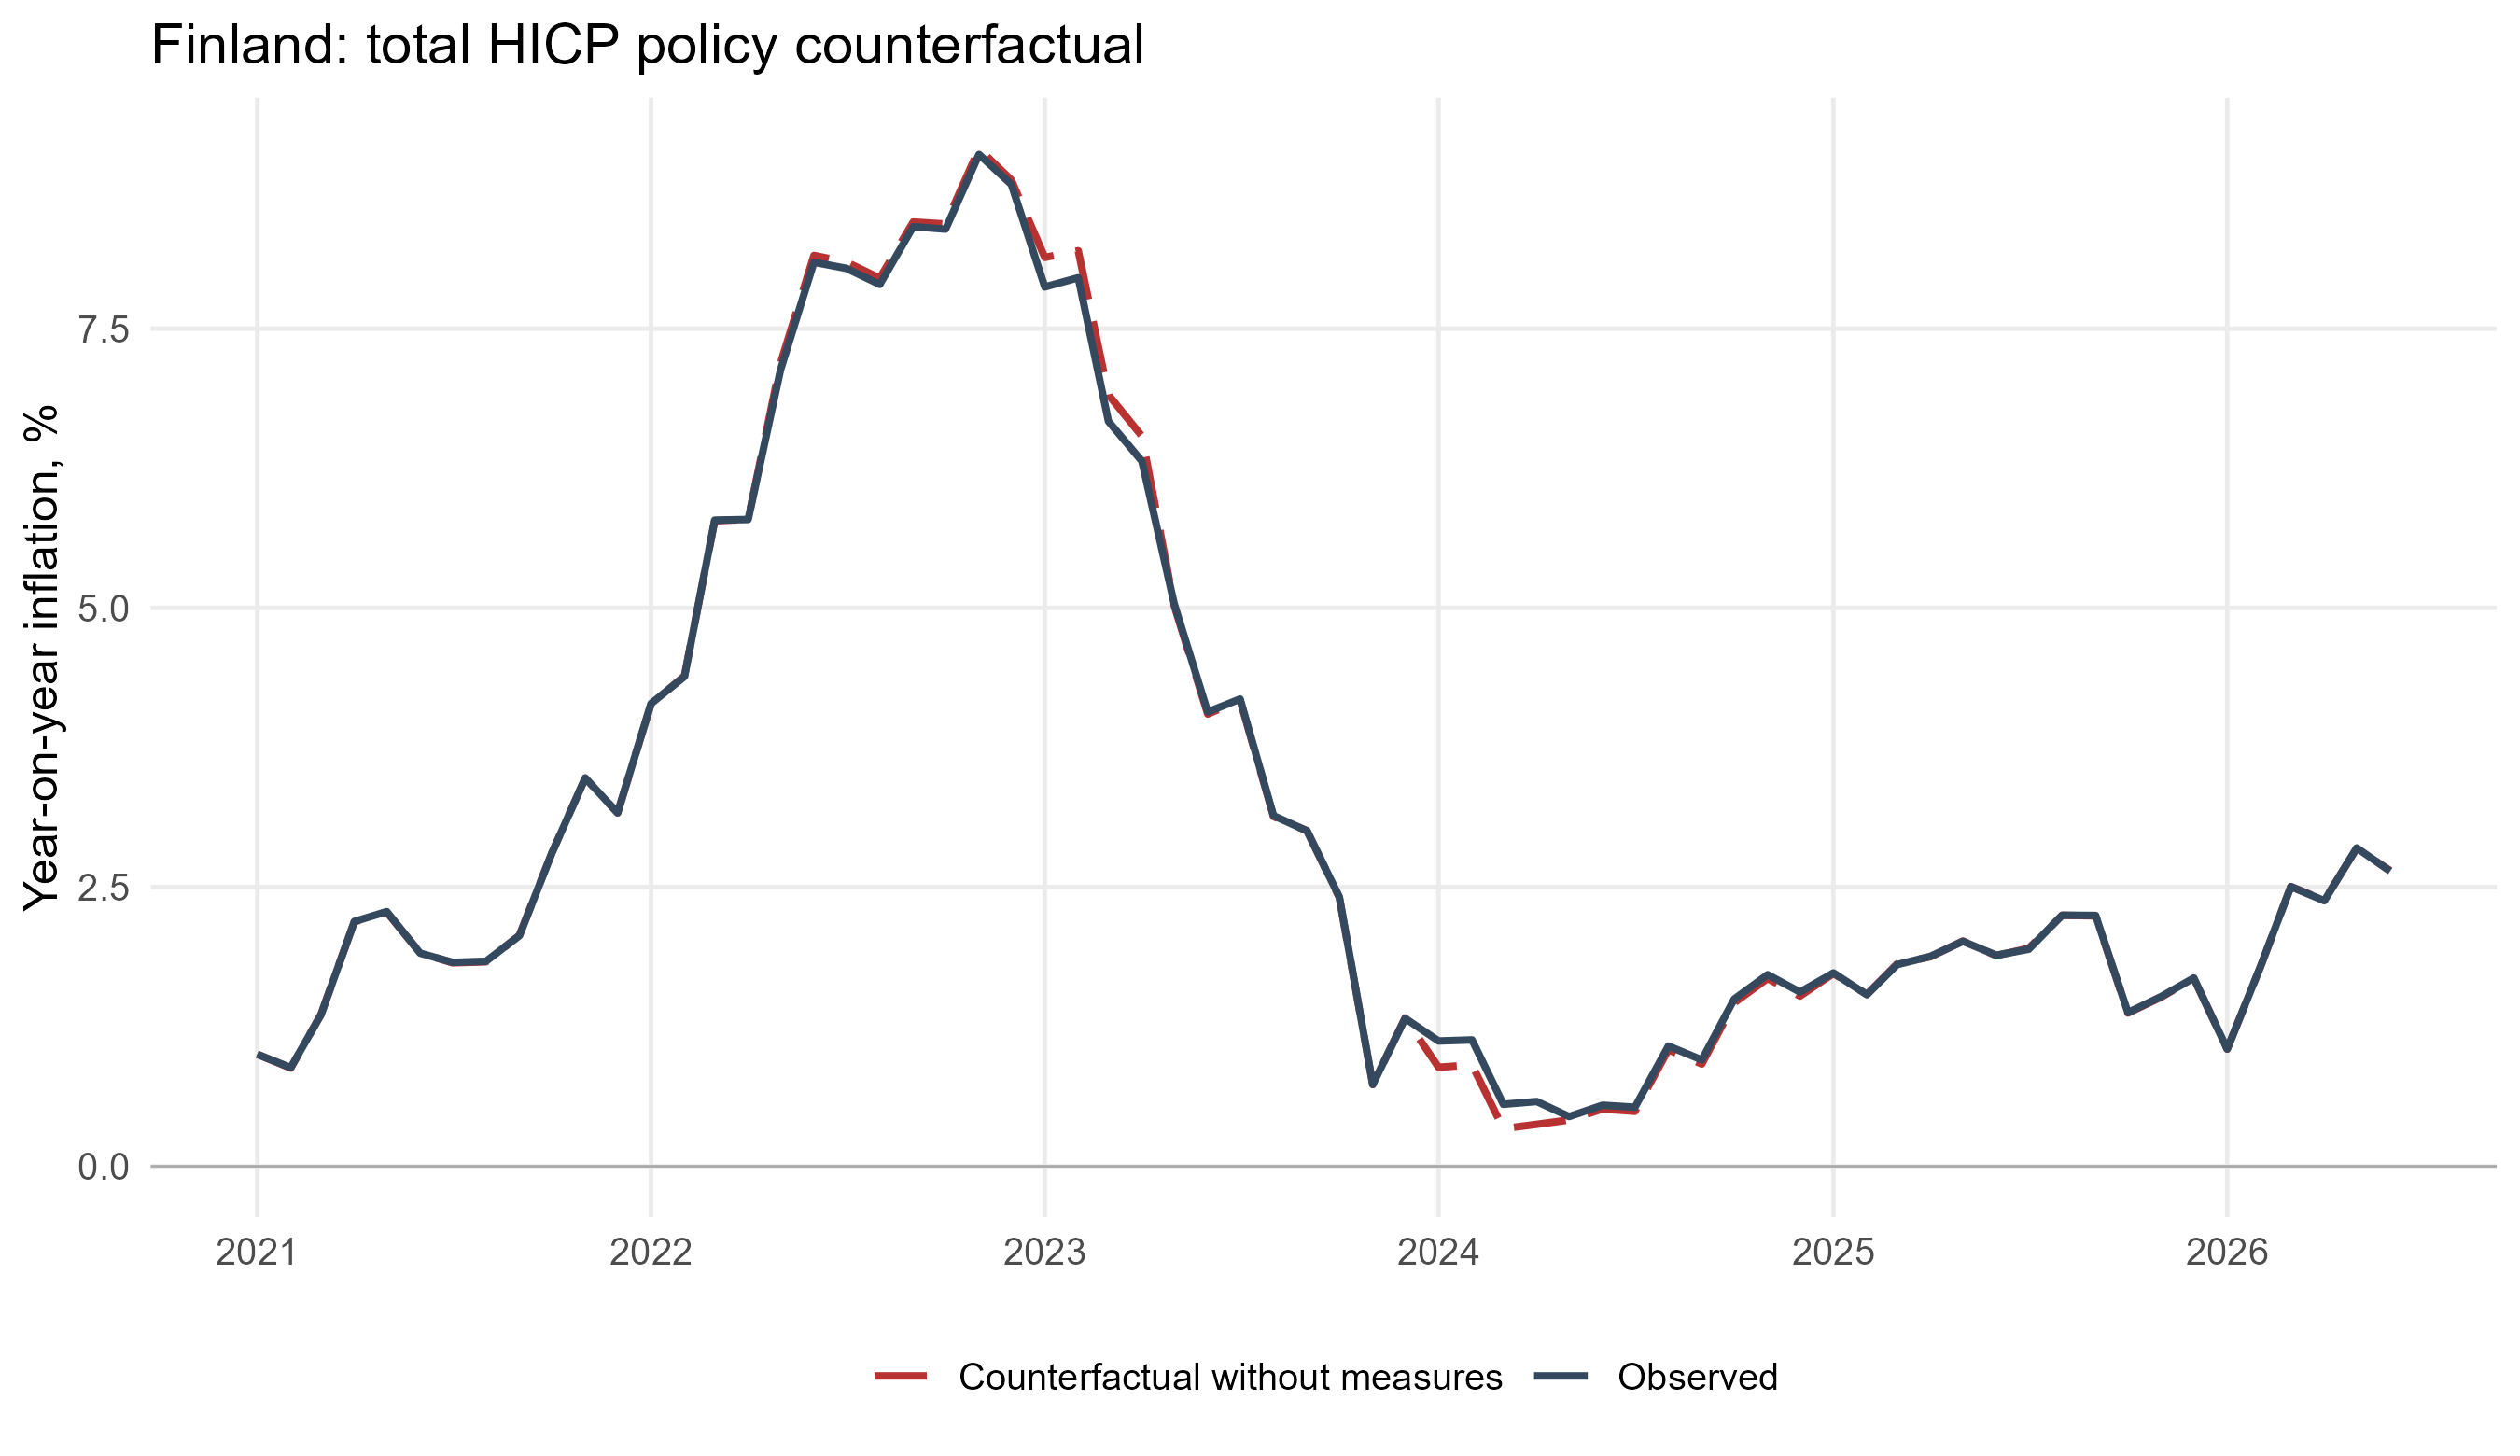
\includegraphics[width=0.86\textwidth,height=0.38\textheight,keepaspectratio]{fig/policy_total_cpi_counterfactual_inflation_FI_finland.png}
\caption{Finland: observed and counterfactual inflation}
\end{figure}

\subsection{France}
\begin{figure}[H]
\centering
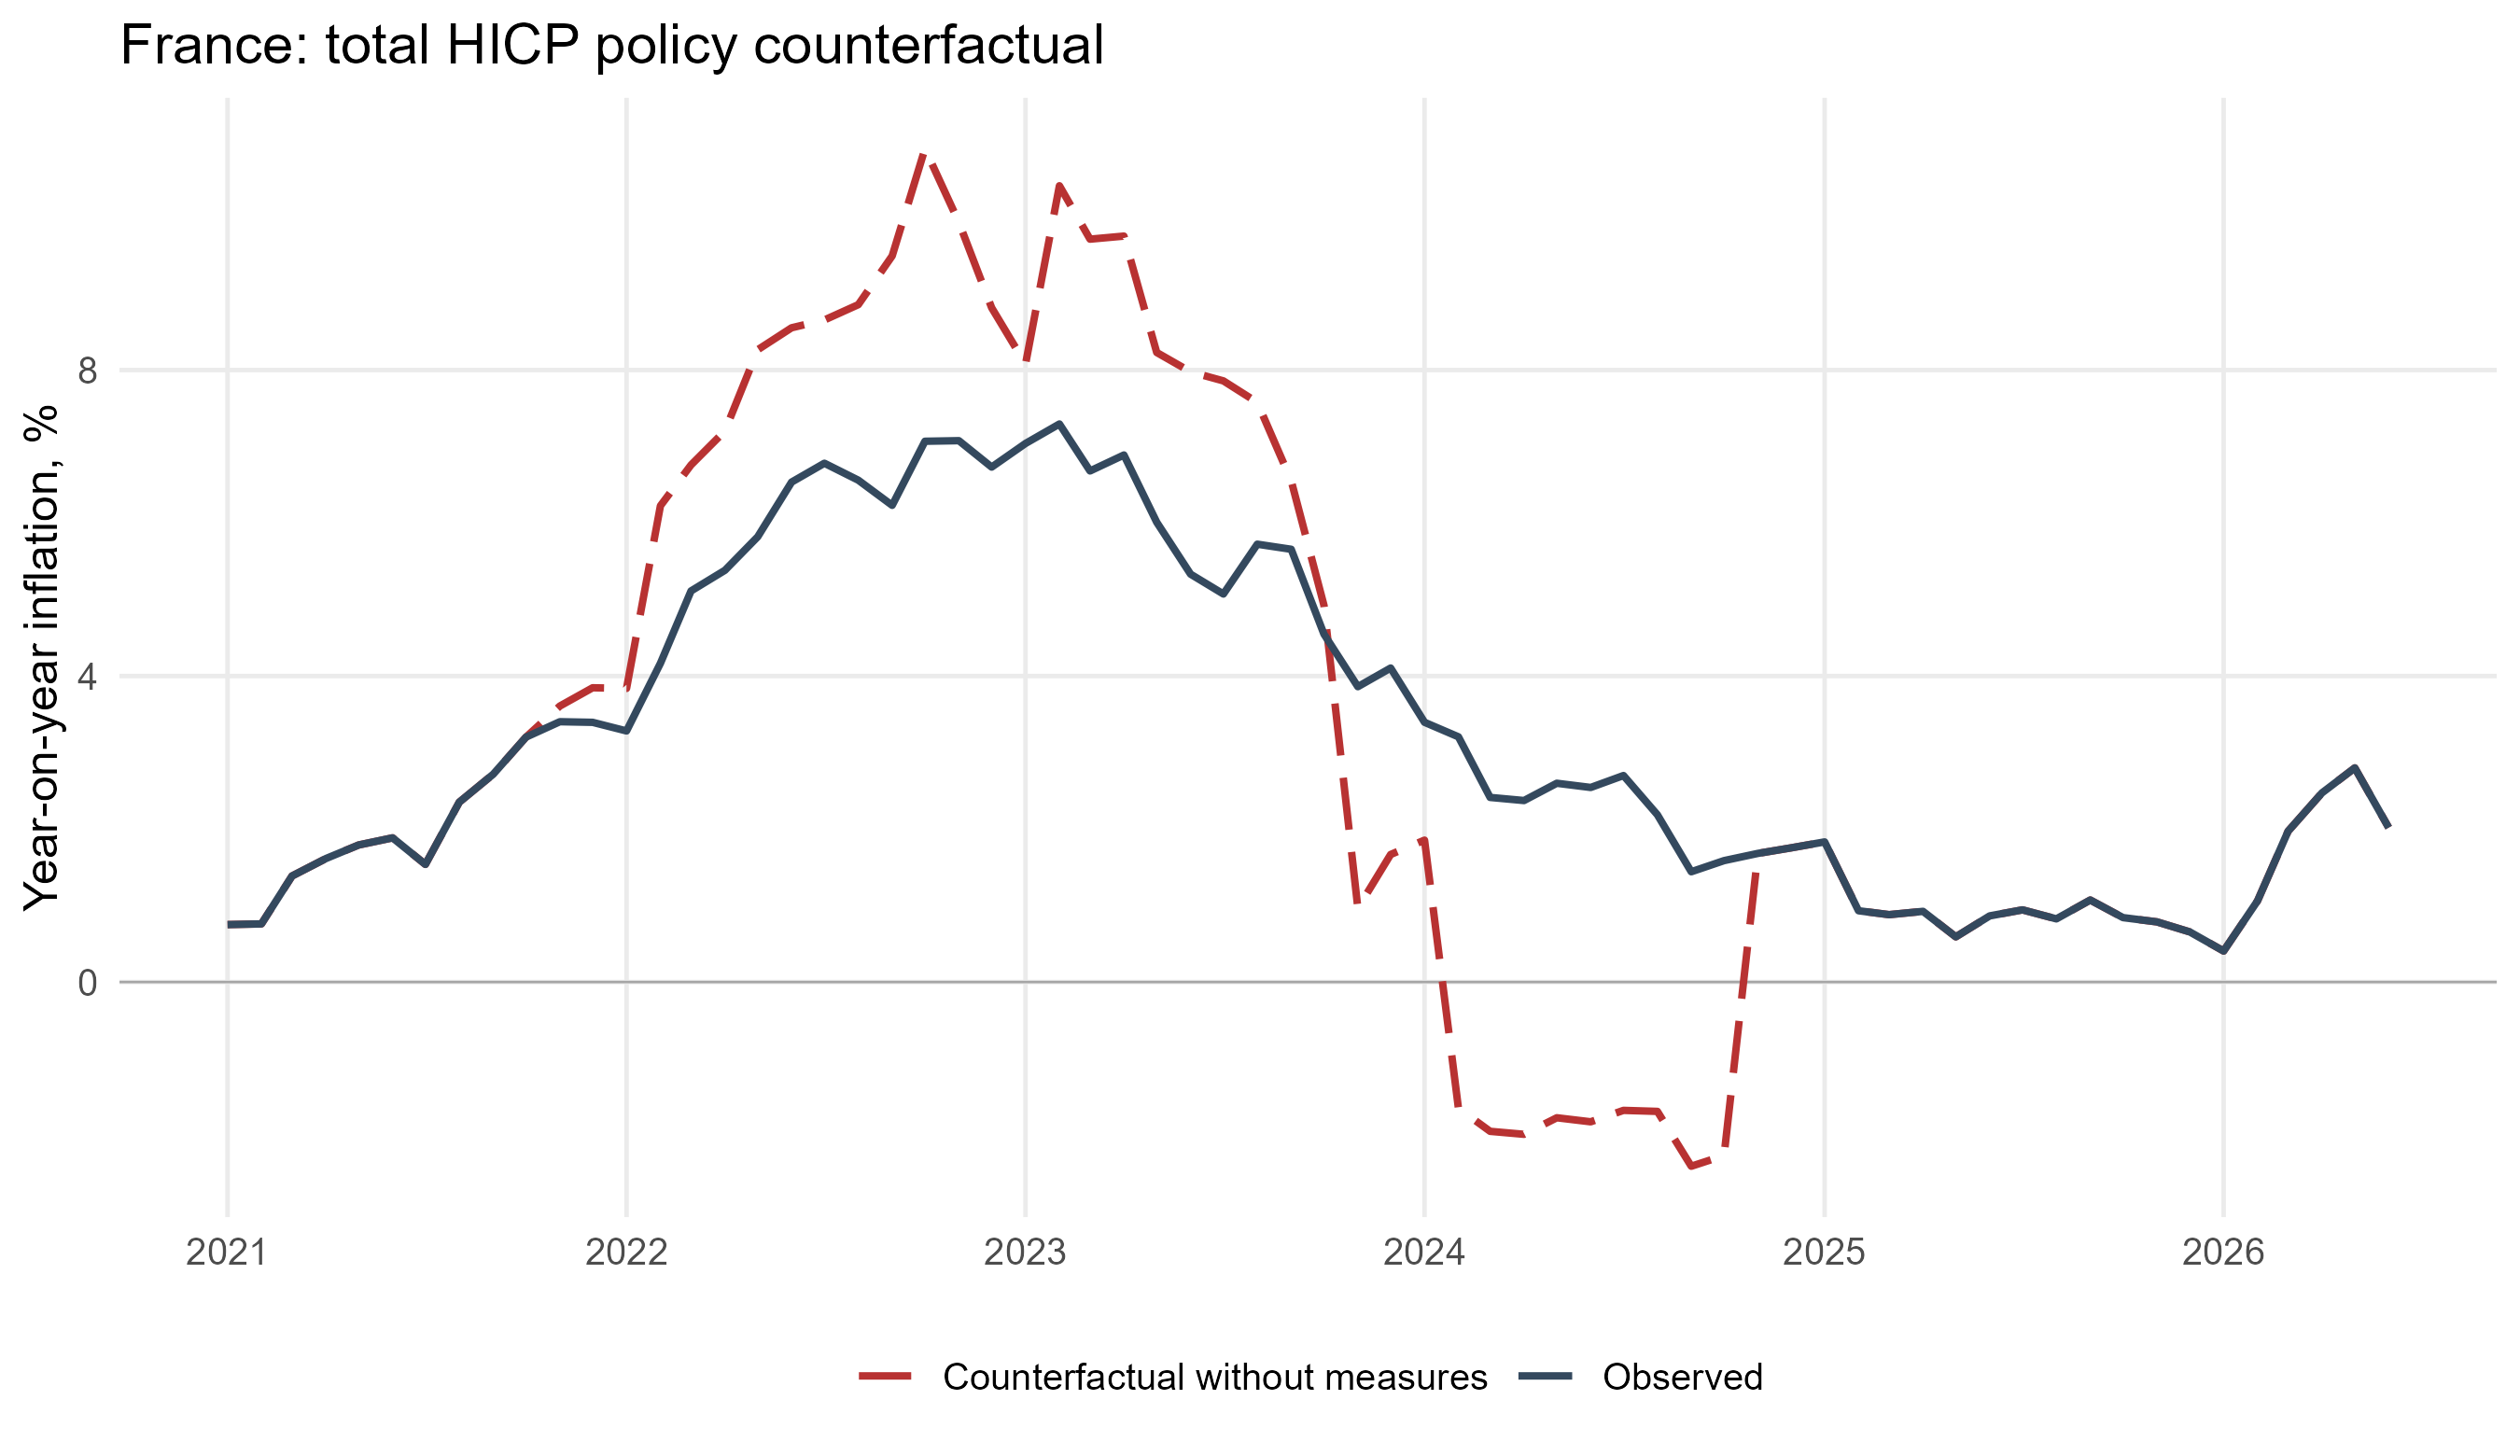
\includegraphics[width=0.86\textwidth,height=0.38\textheight,keepaspectratio]{fig/policy_total_cpi_counterfactual_inflation_FR_france.png}
\caption{France: observed and counterfactual inflation}
\end{figure}

\subsection{Croatia}
\begin{figure}[H]
\centering
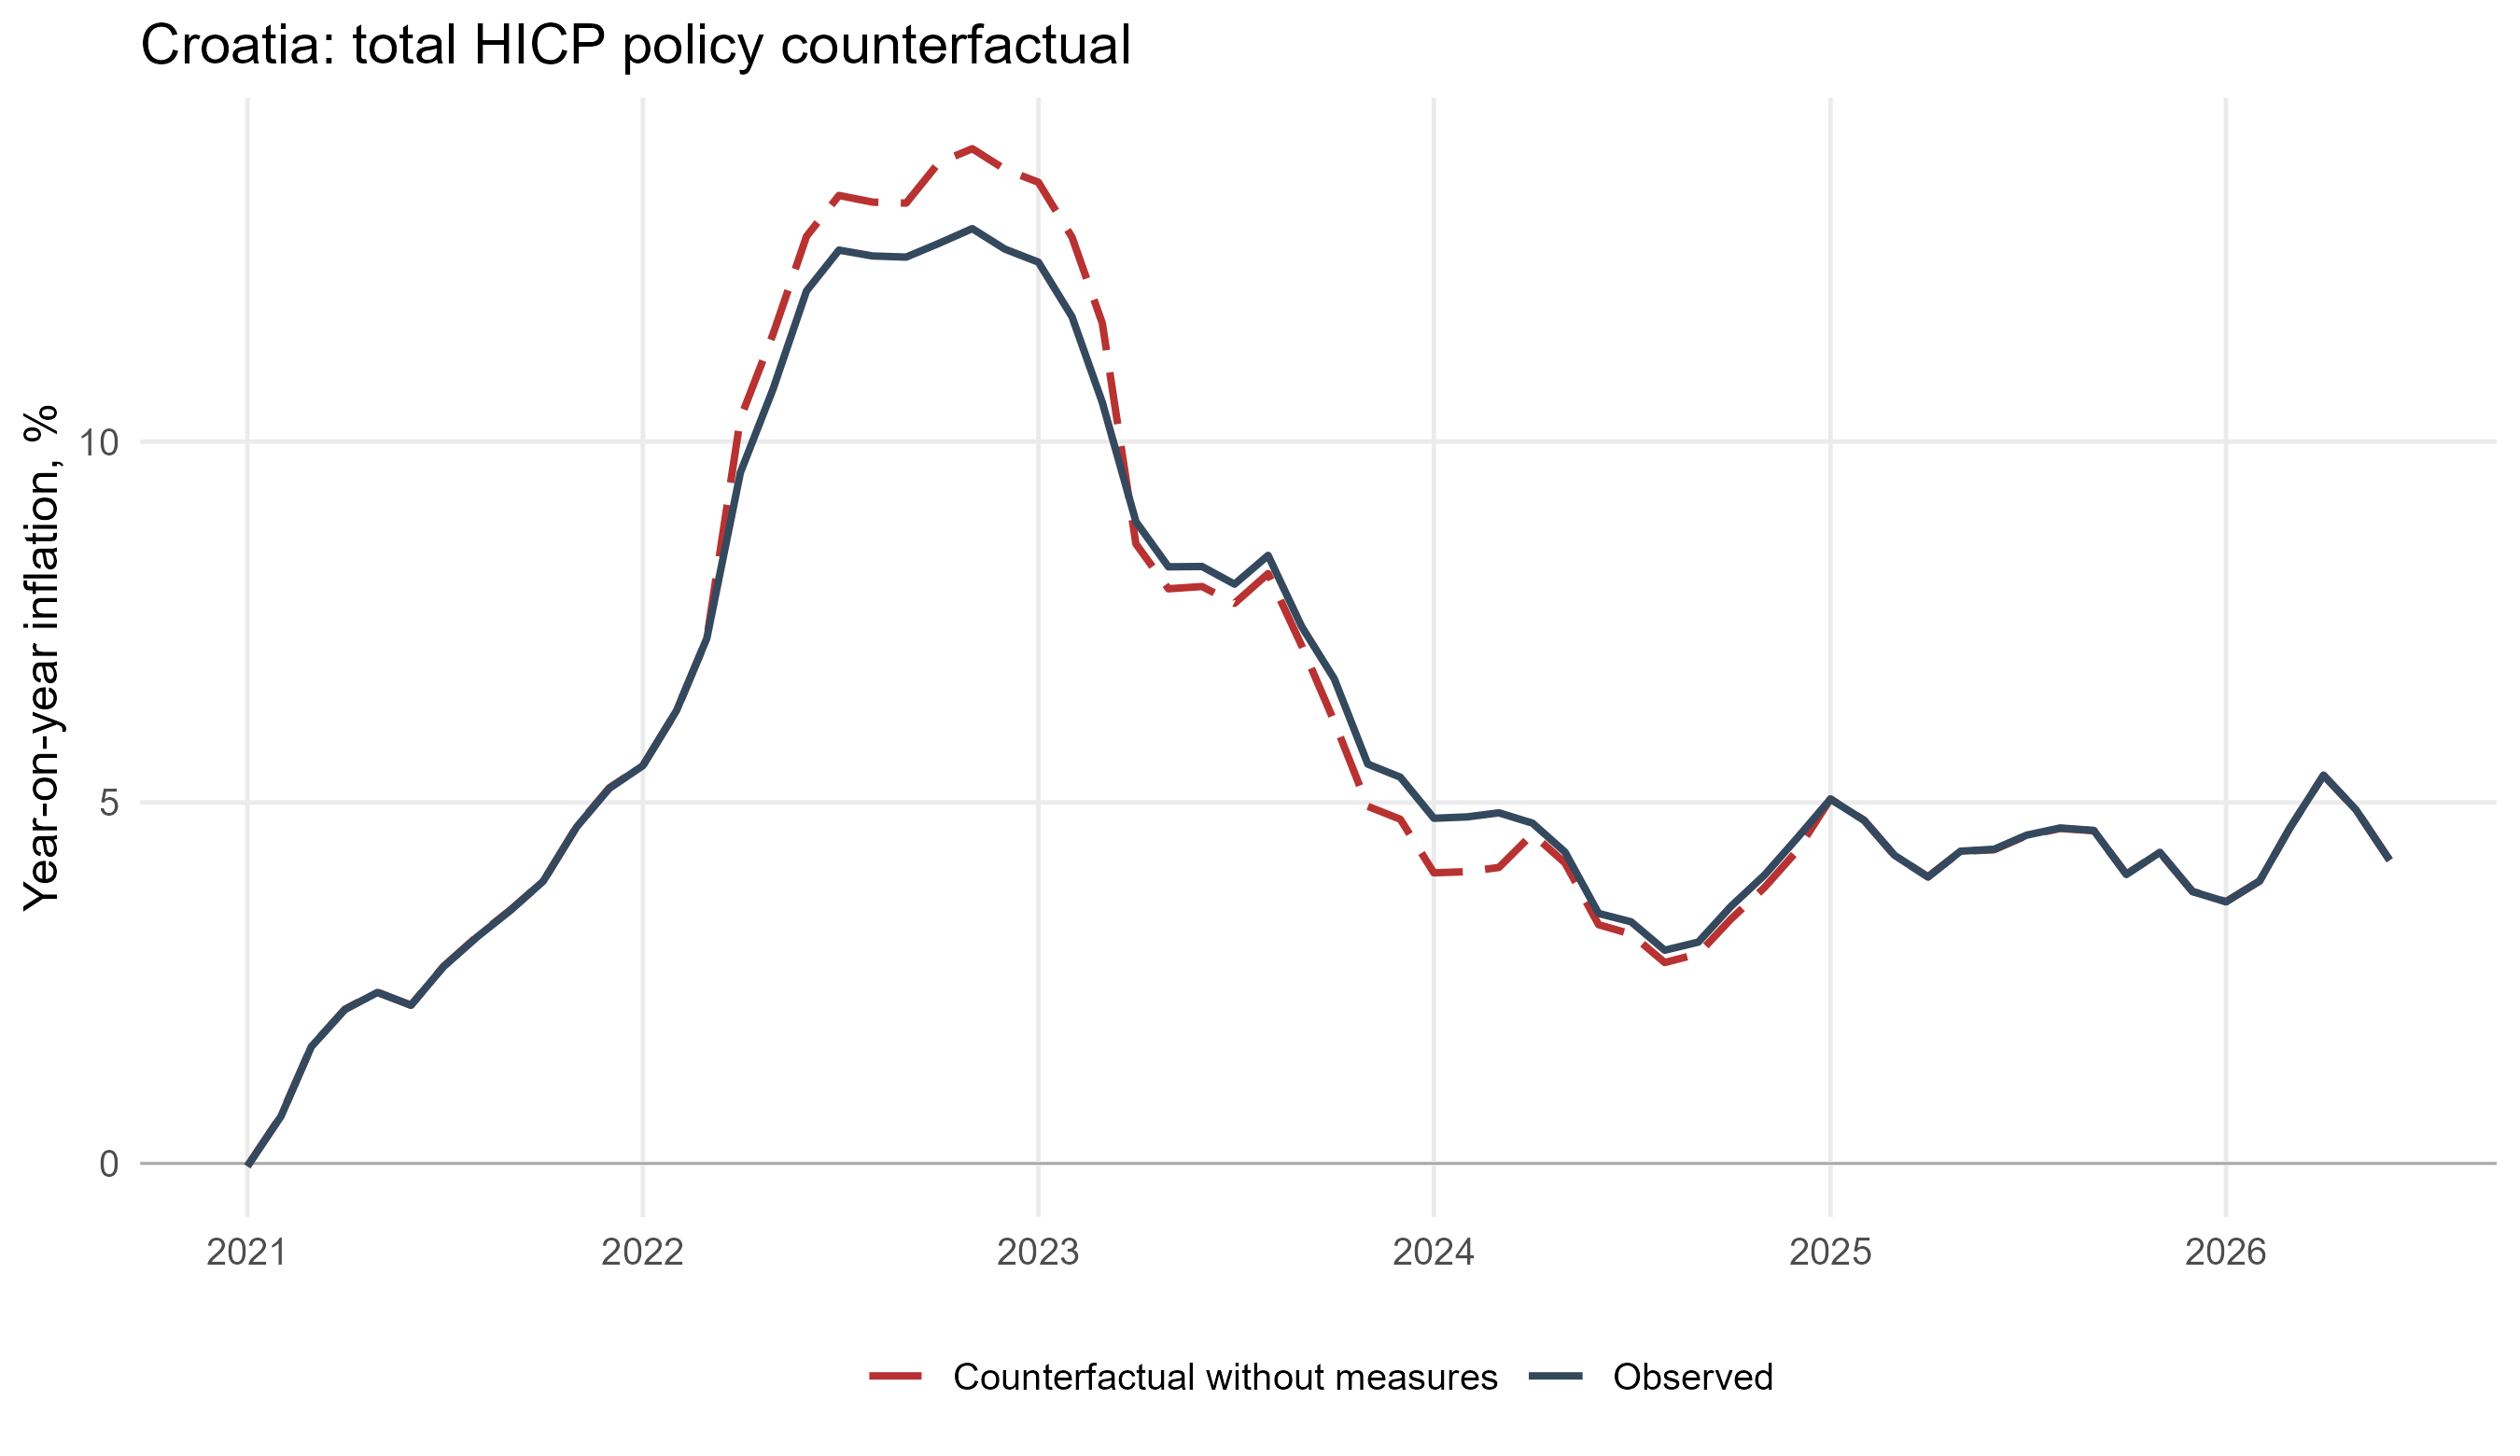
\includegraphics[width=0.86\textwidth,height=0.38\textheight,keepaspectratio]{fig/policy_total_cpi_counterfactual_inflation_HR_croatia.png}
\caption{Croatia: observed and counterfactual inflation}
\end{figure}

\subsection{Ireland}
\begin{figure}[H]
\centering
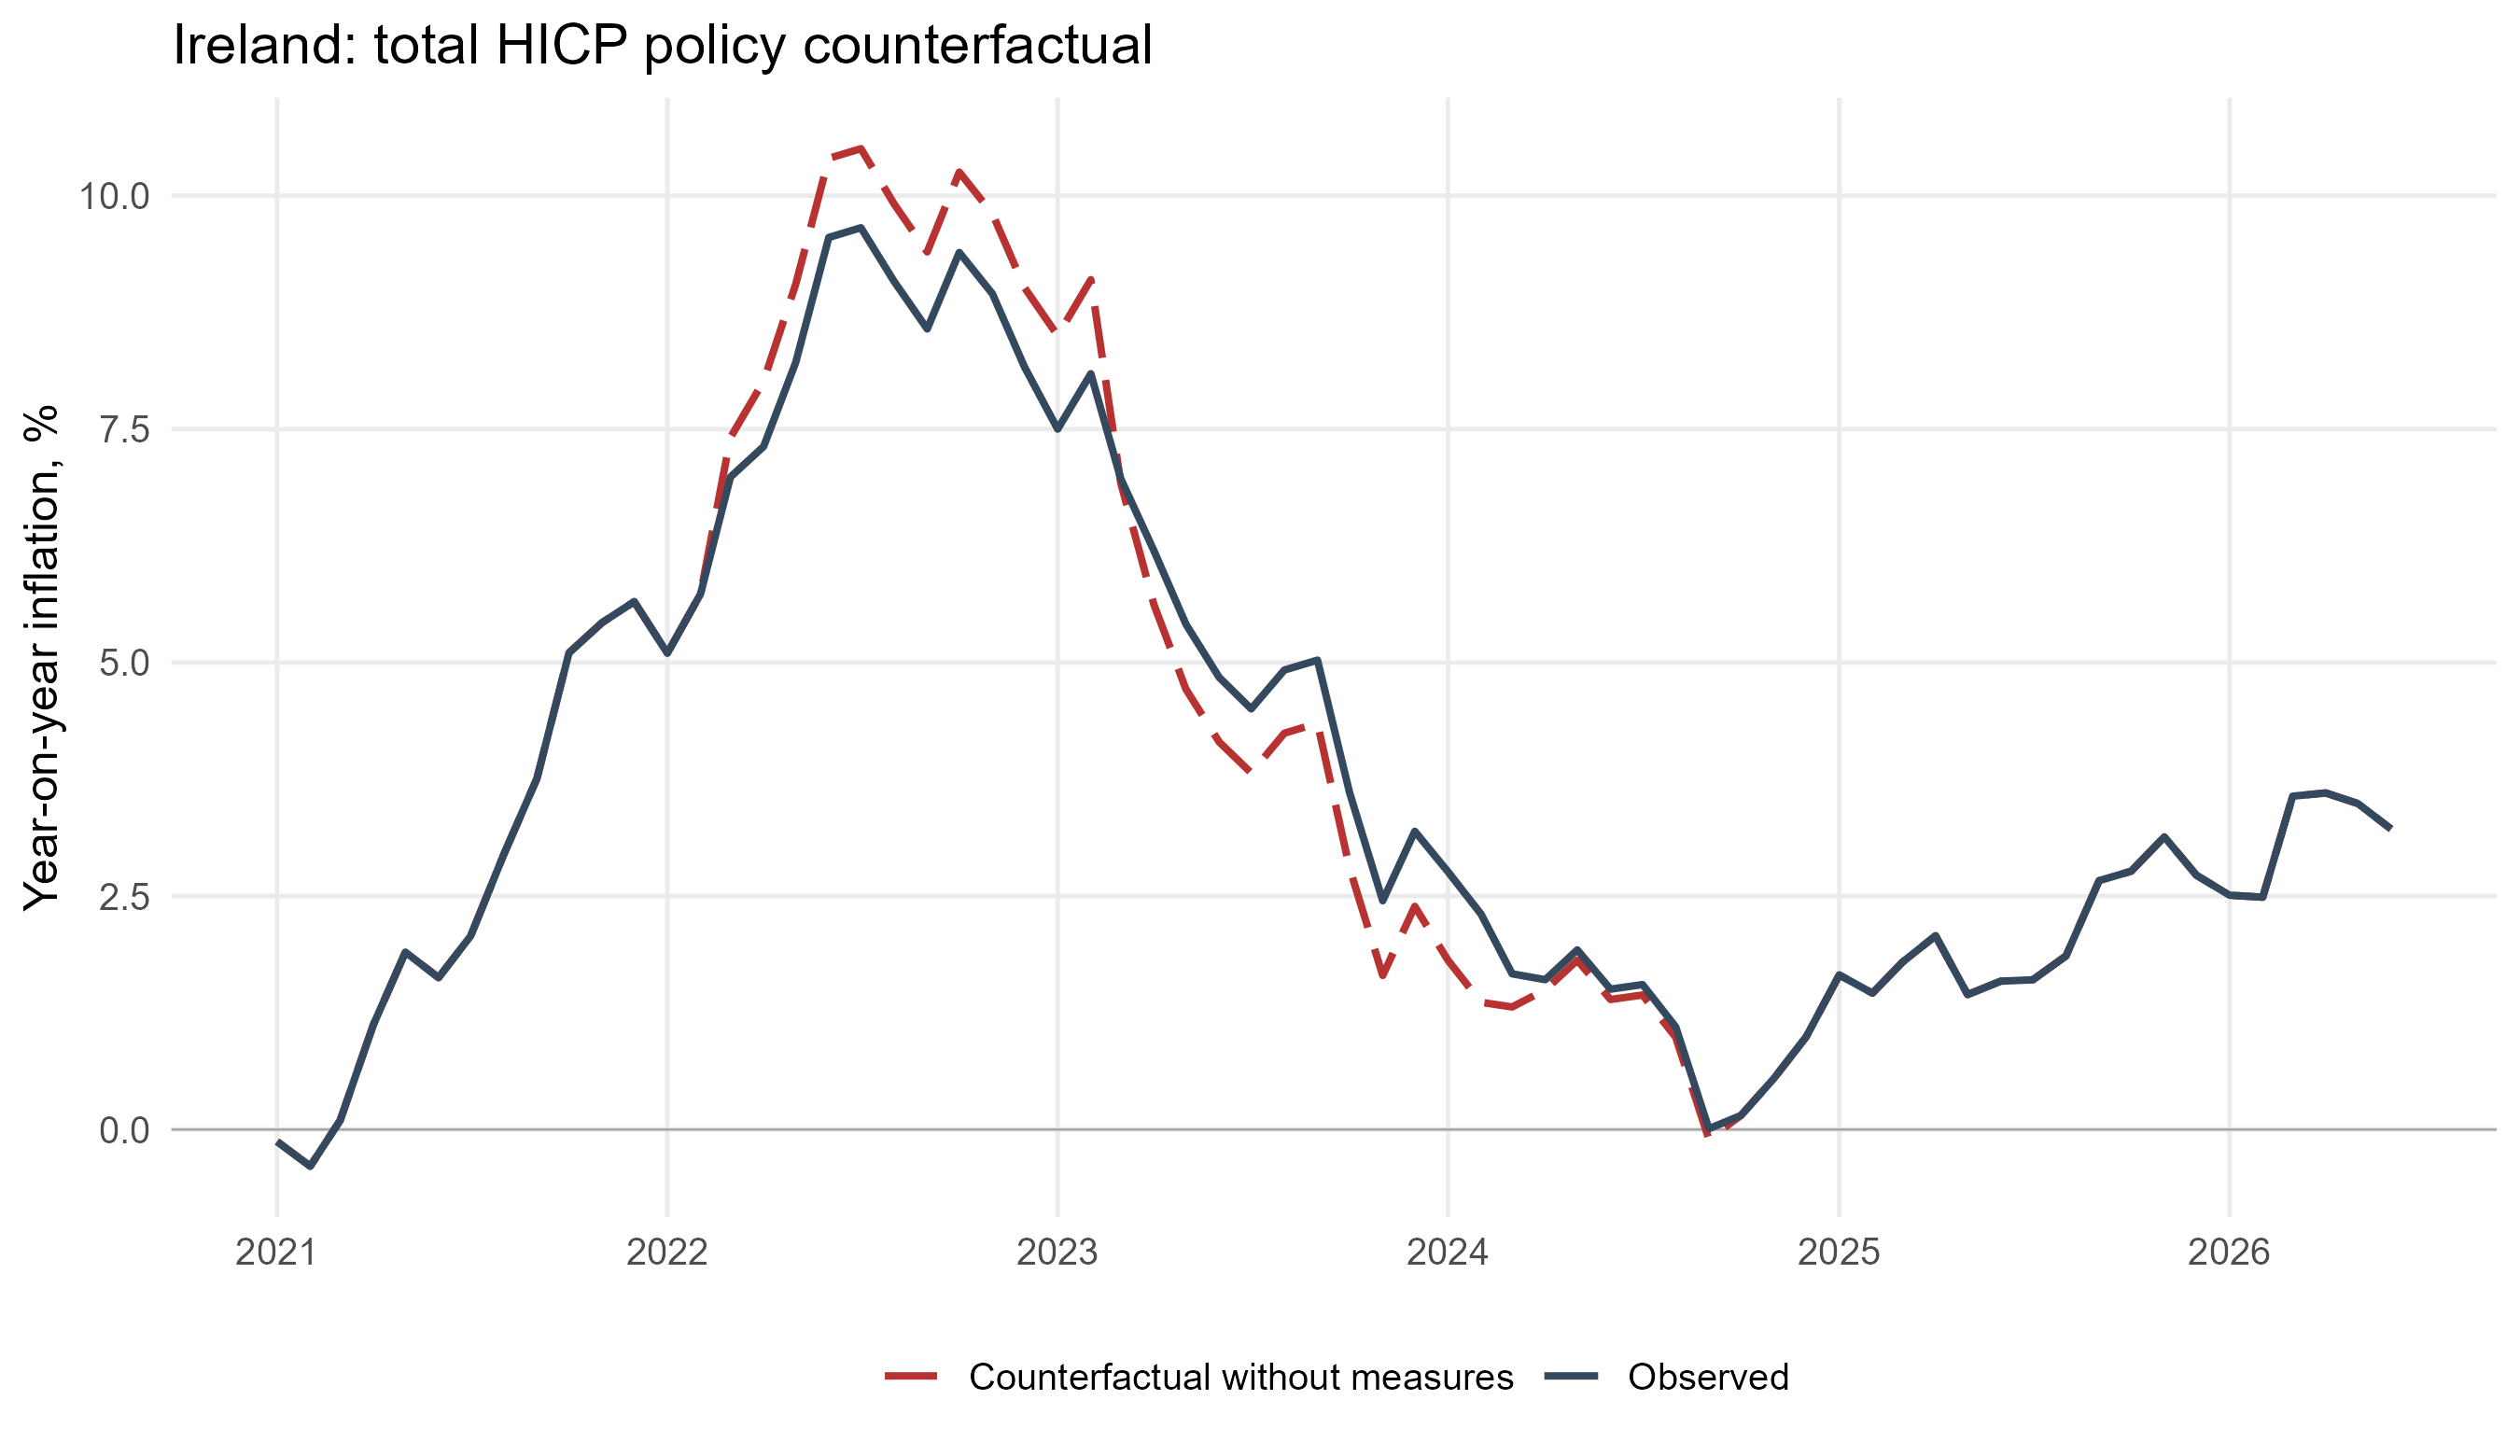
\includegraphics[width=0.86\textwidth,height=0.38\textheight,keepaspectratio]{fig/policy_total_cpi_counterfactual_inflation_IE_ireland.png}
\caption{Ireland: observed and counterfactual inflation}
\end{figure}

\subsection{Italy}
\begin{figure}[H]
\centering
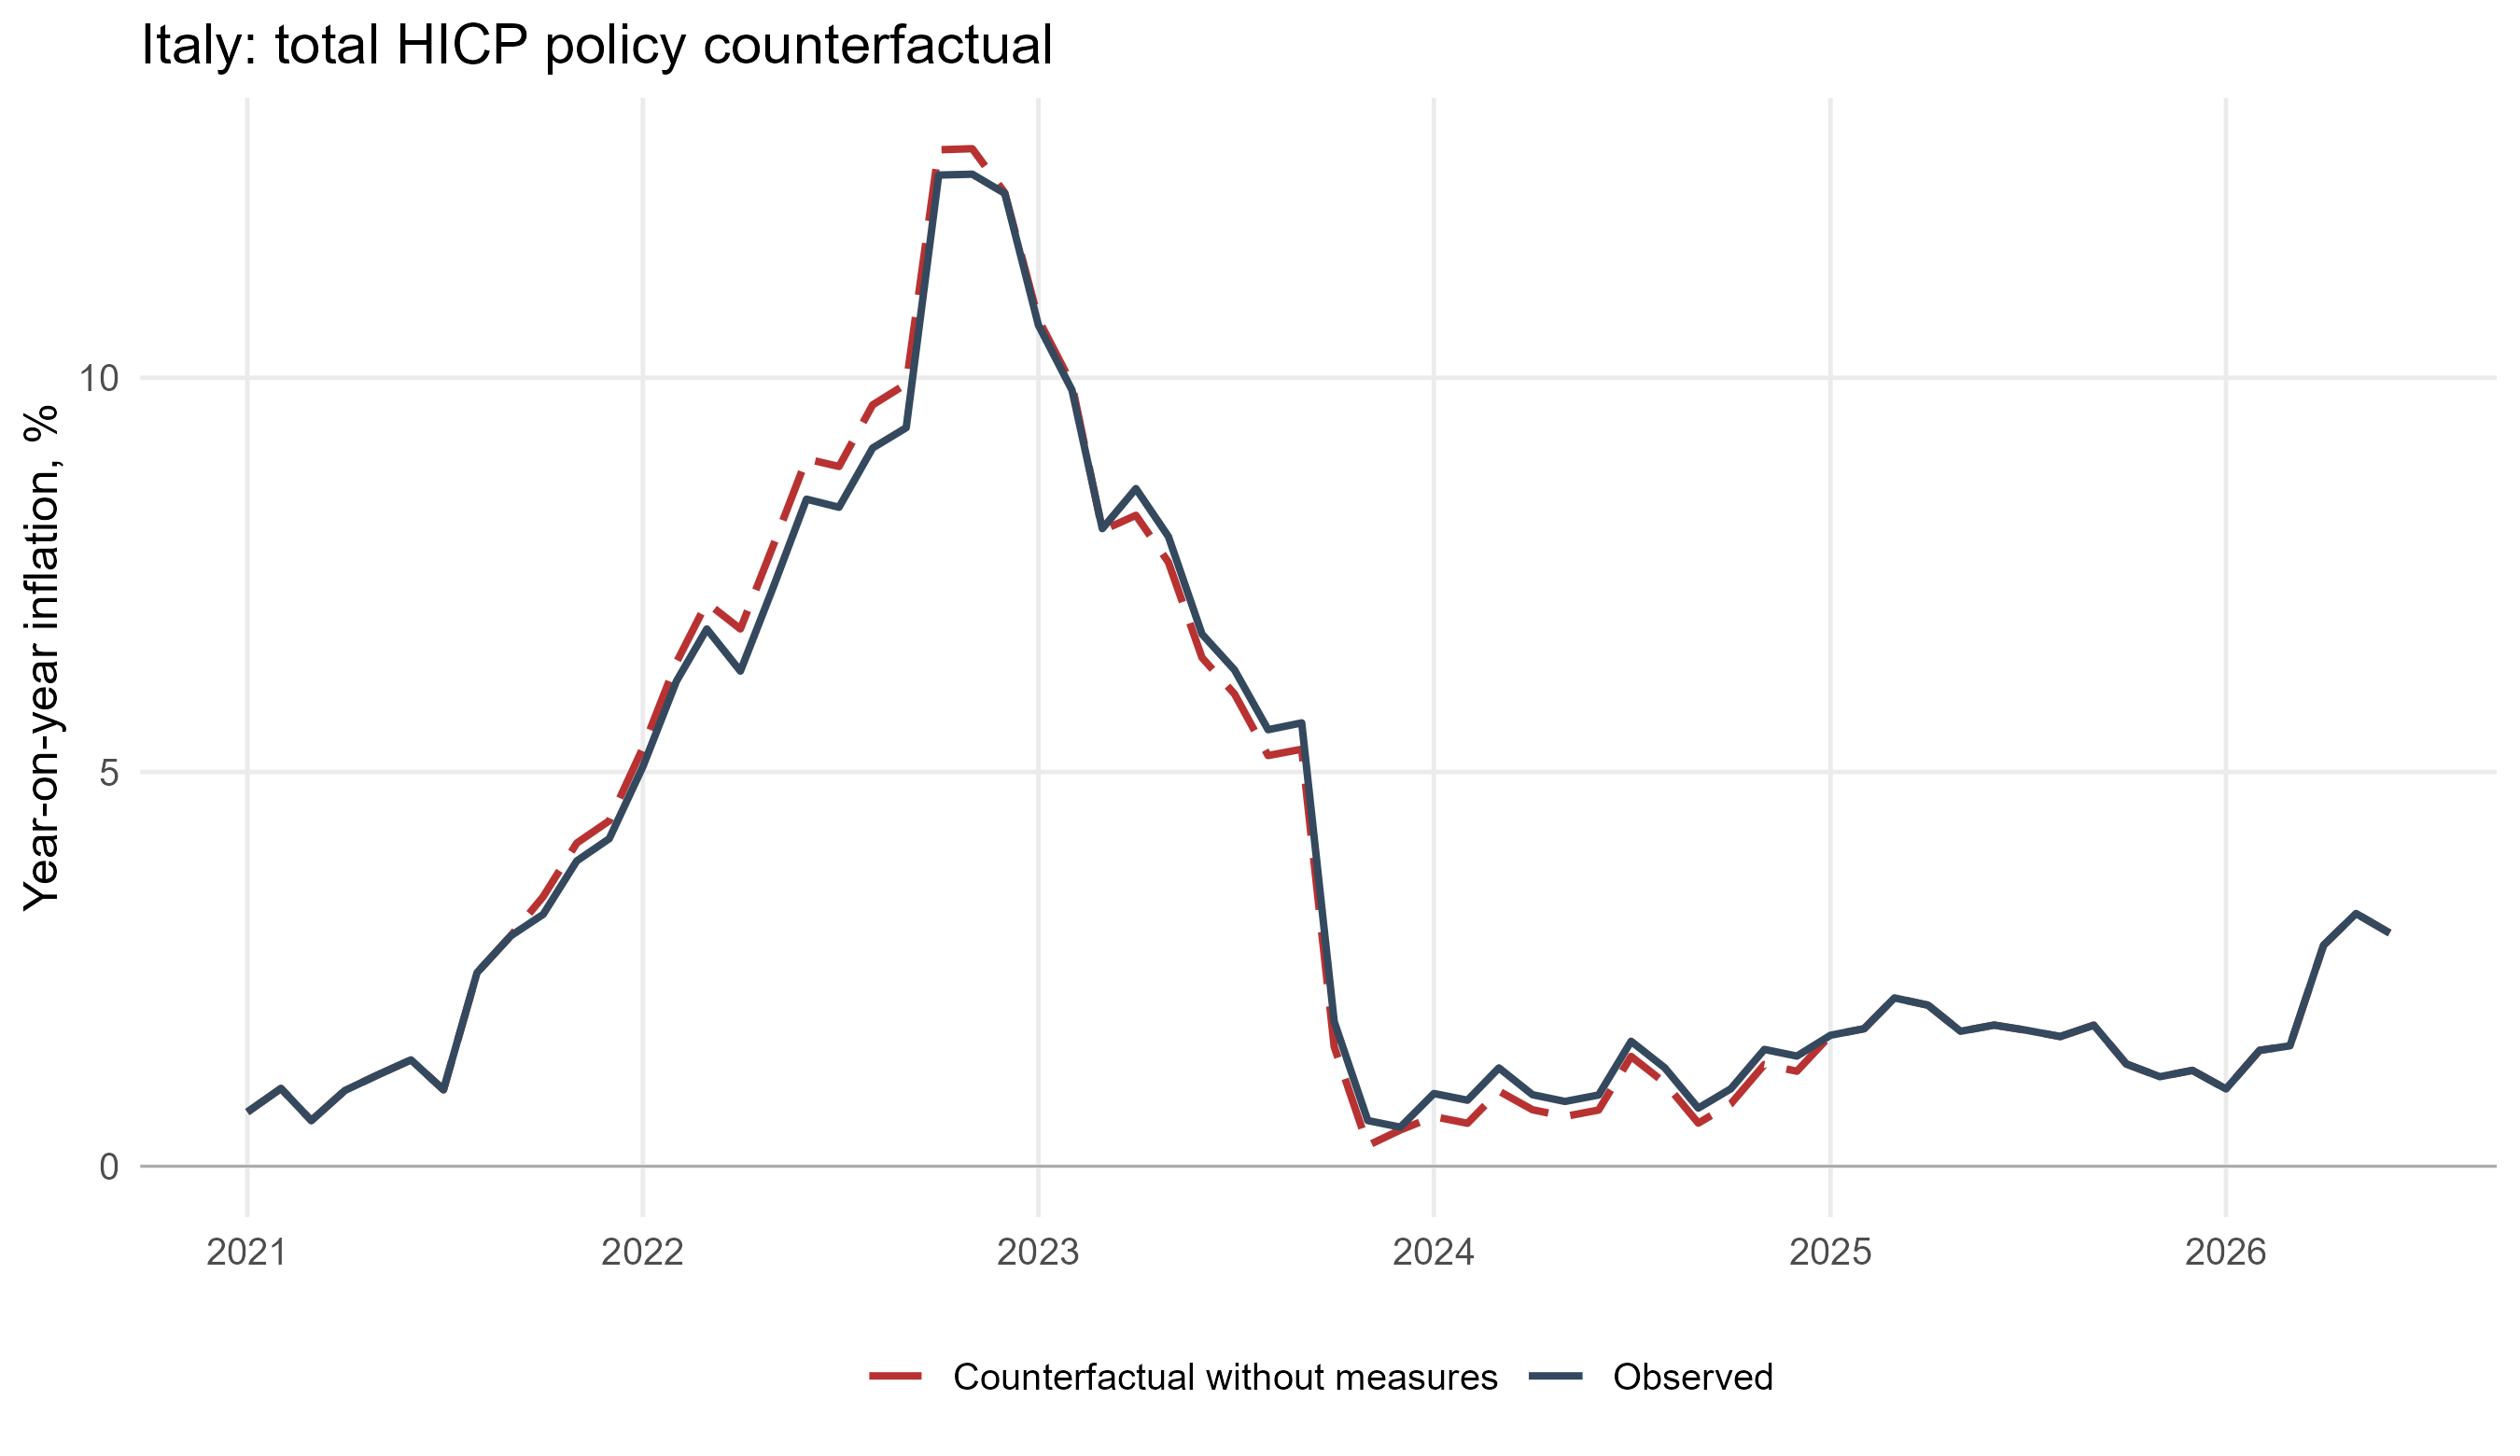
\includegraphics[width=0.86\textwidth,height=0.38\textheight,keepaspectratio]{fig/policy_total_cpi_counterfactual_inflation_IT_italy.png}
\caption{Italy: observed and counterfactual inflation}
\end{figure}

\subsection{Lithuania}
\begin{figure}[H]
\centering
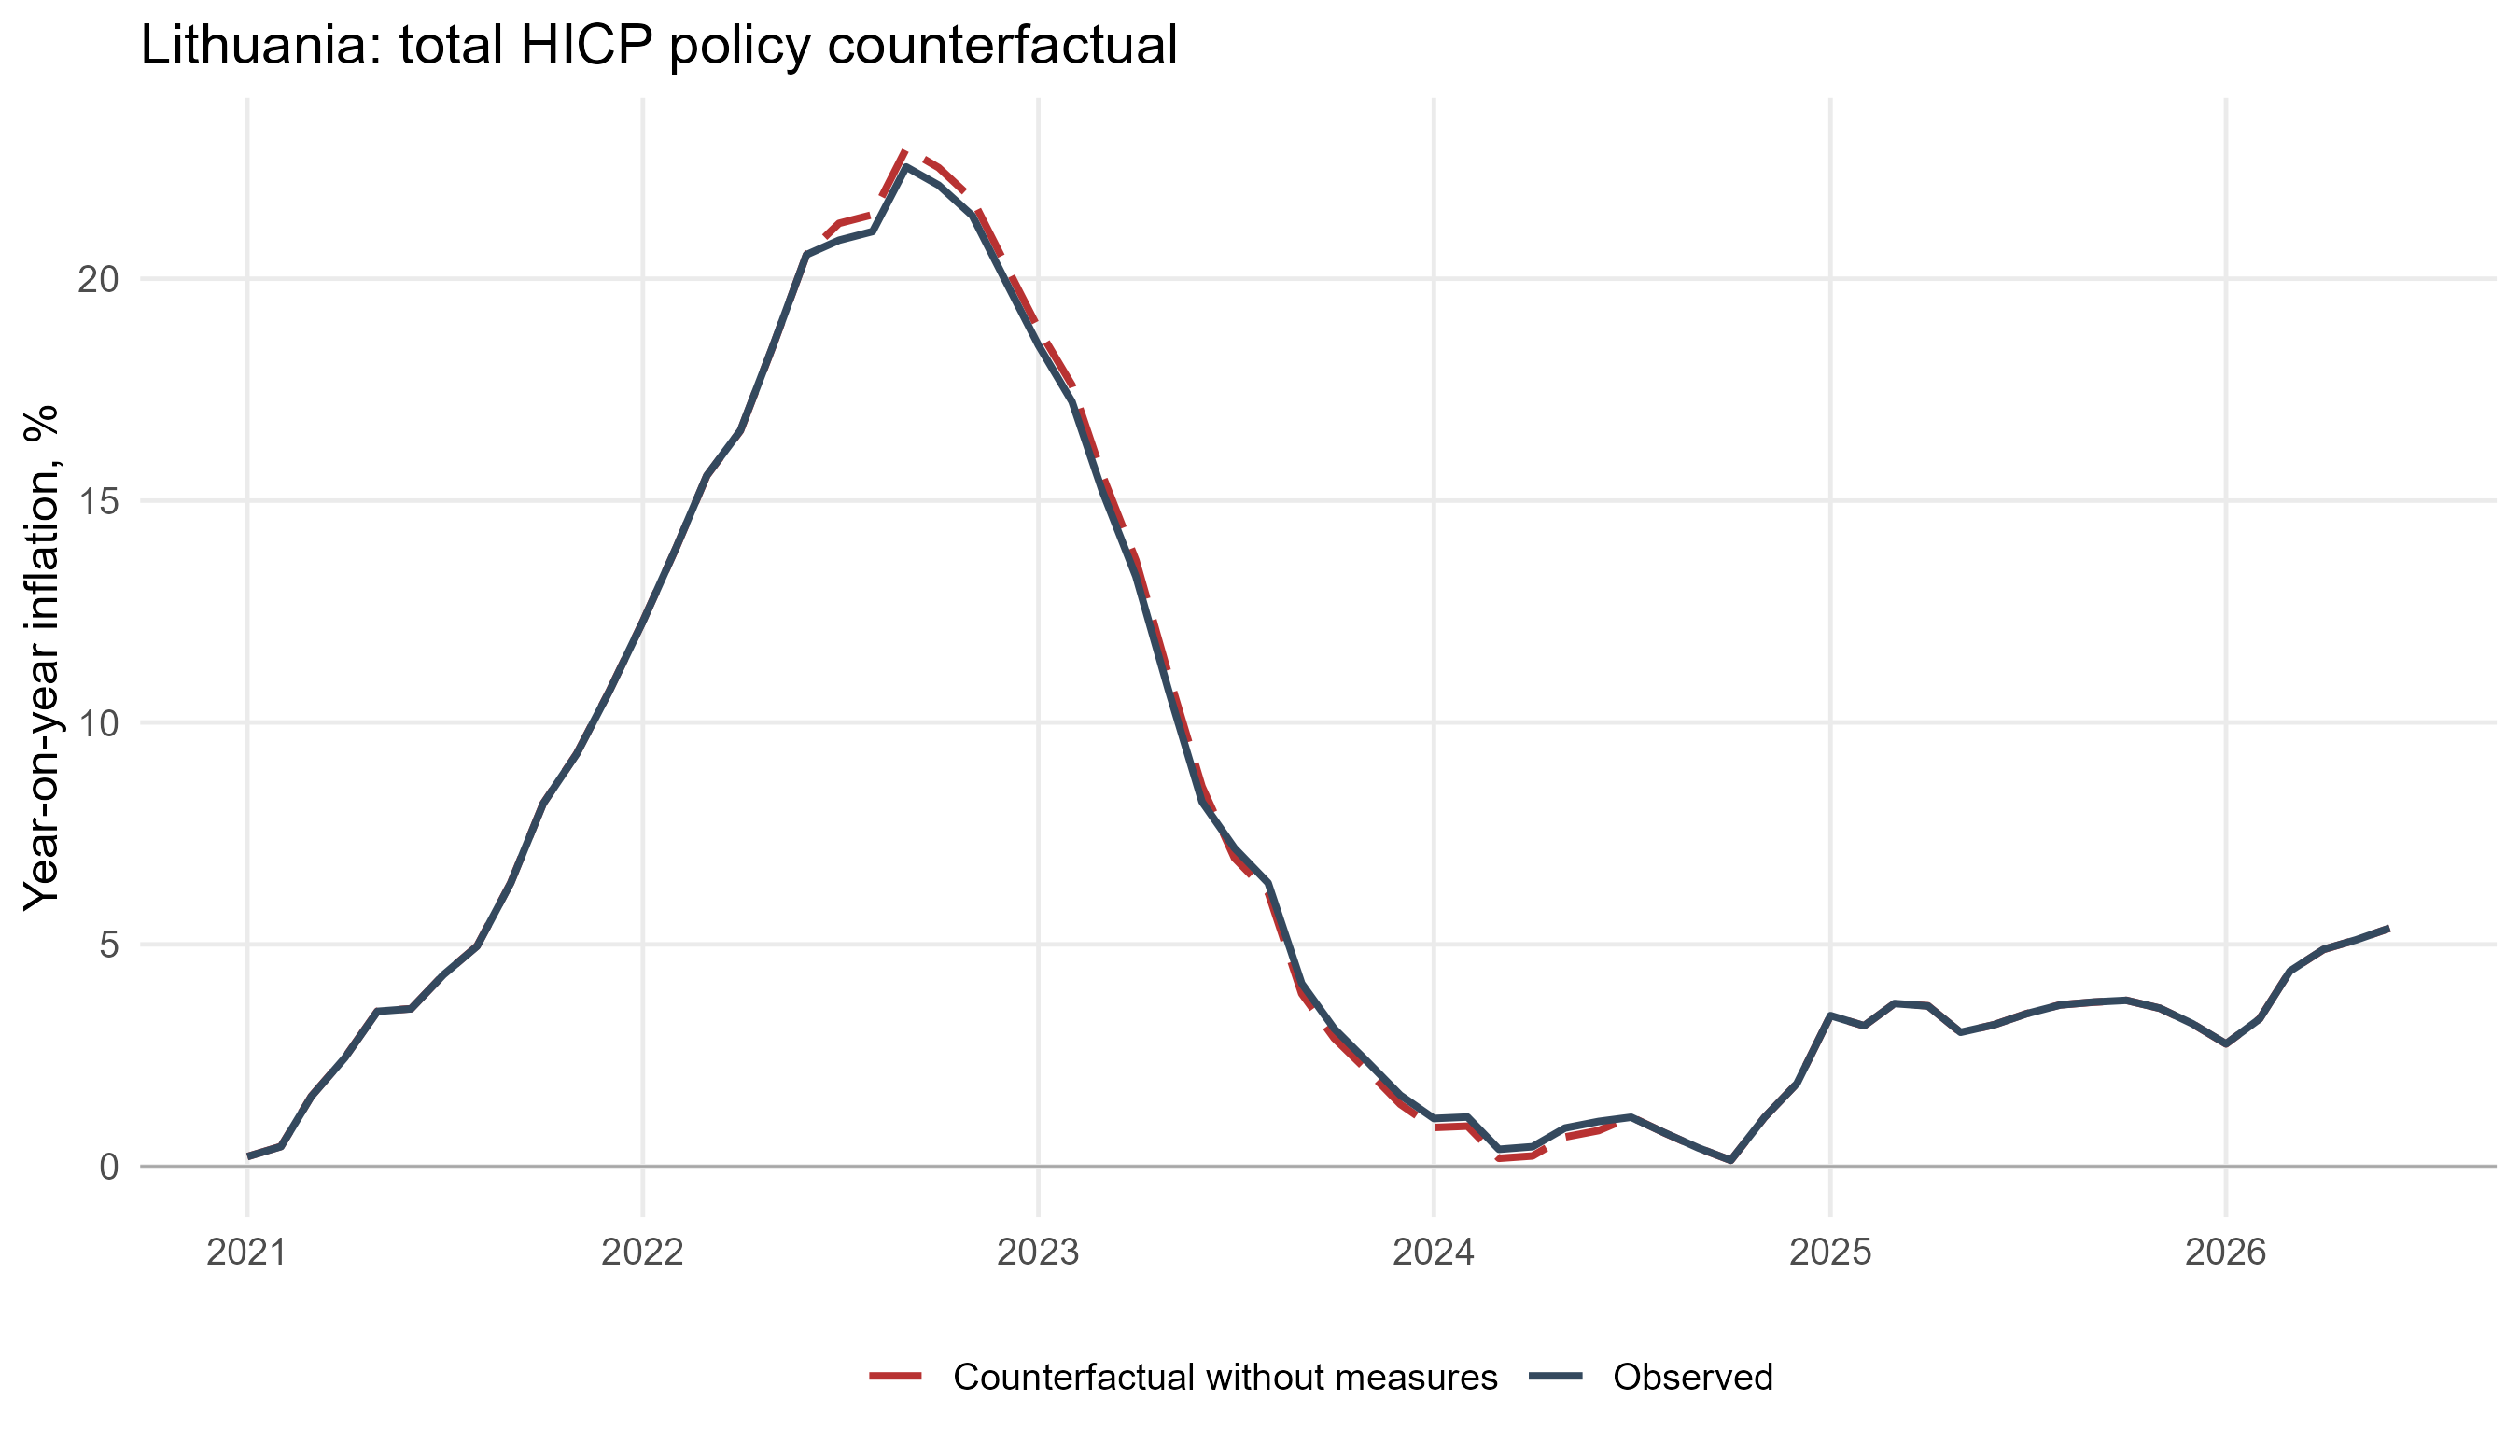
\includegraphics[width=0.86\textwidth,height=0.38\textheight,keepaspectratio]{fig/policy_total_cpi_counterfactual_inflation_LT_lithuania.png}
\caption{Lithuania: observed and counterfactual inflation}
\end{figure}

\subsection{Luxembourg}
\begin{figure}[H]
\centering
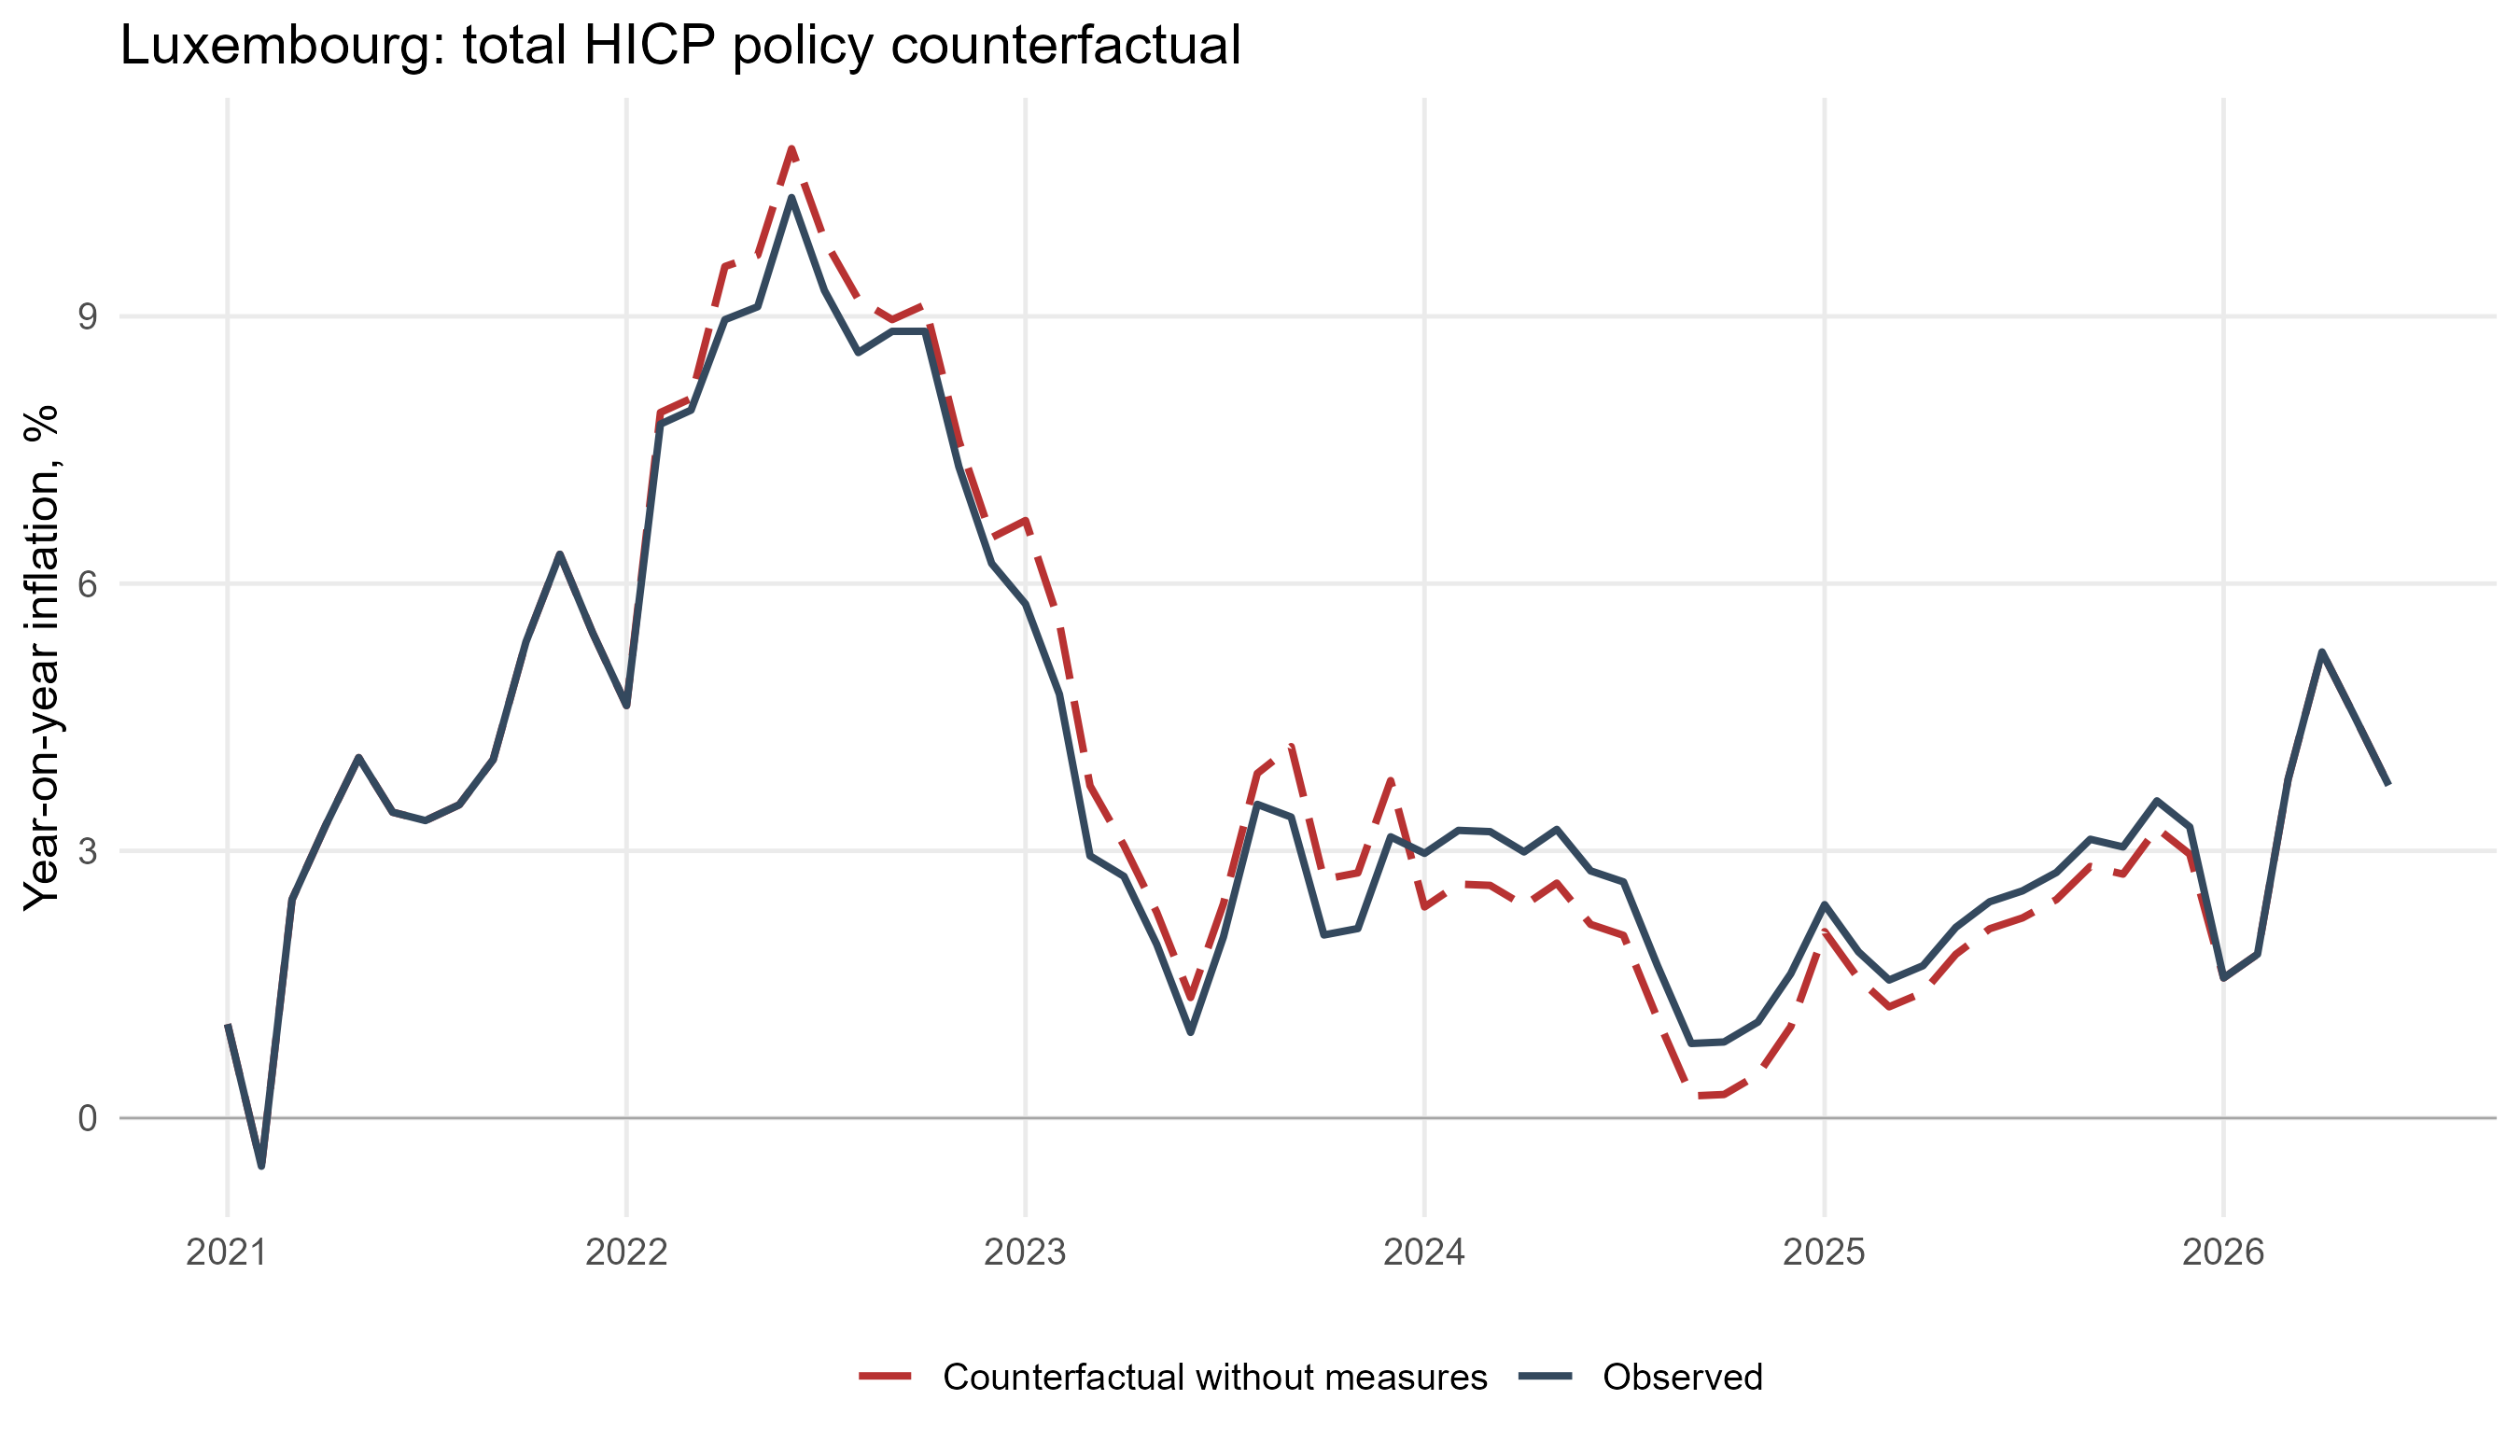
\includegraphics[width=0.86\textwidth,height=0.38\textheight,keepaspectratio]{fig/policy_total_cpi_counterfactual_inflation_LU_luxembourg.png}
\caption{Luxembourg: observed and counterfactual inflation}
\end{figure}

\subsection{Latvia}
\begin{figure}[H]
\centering
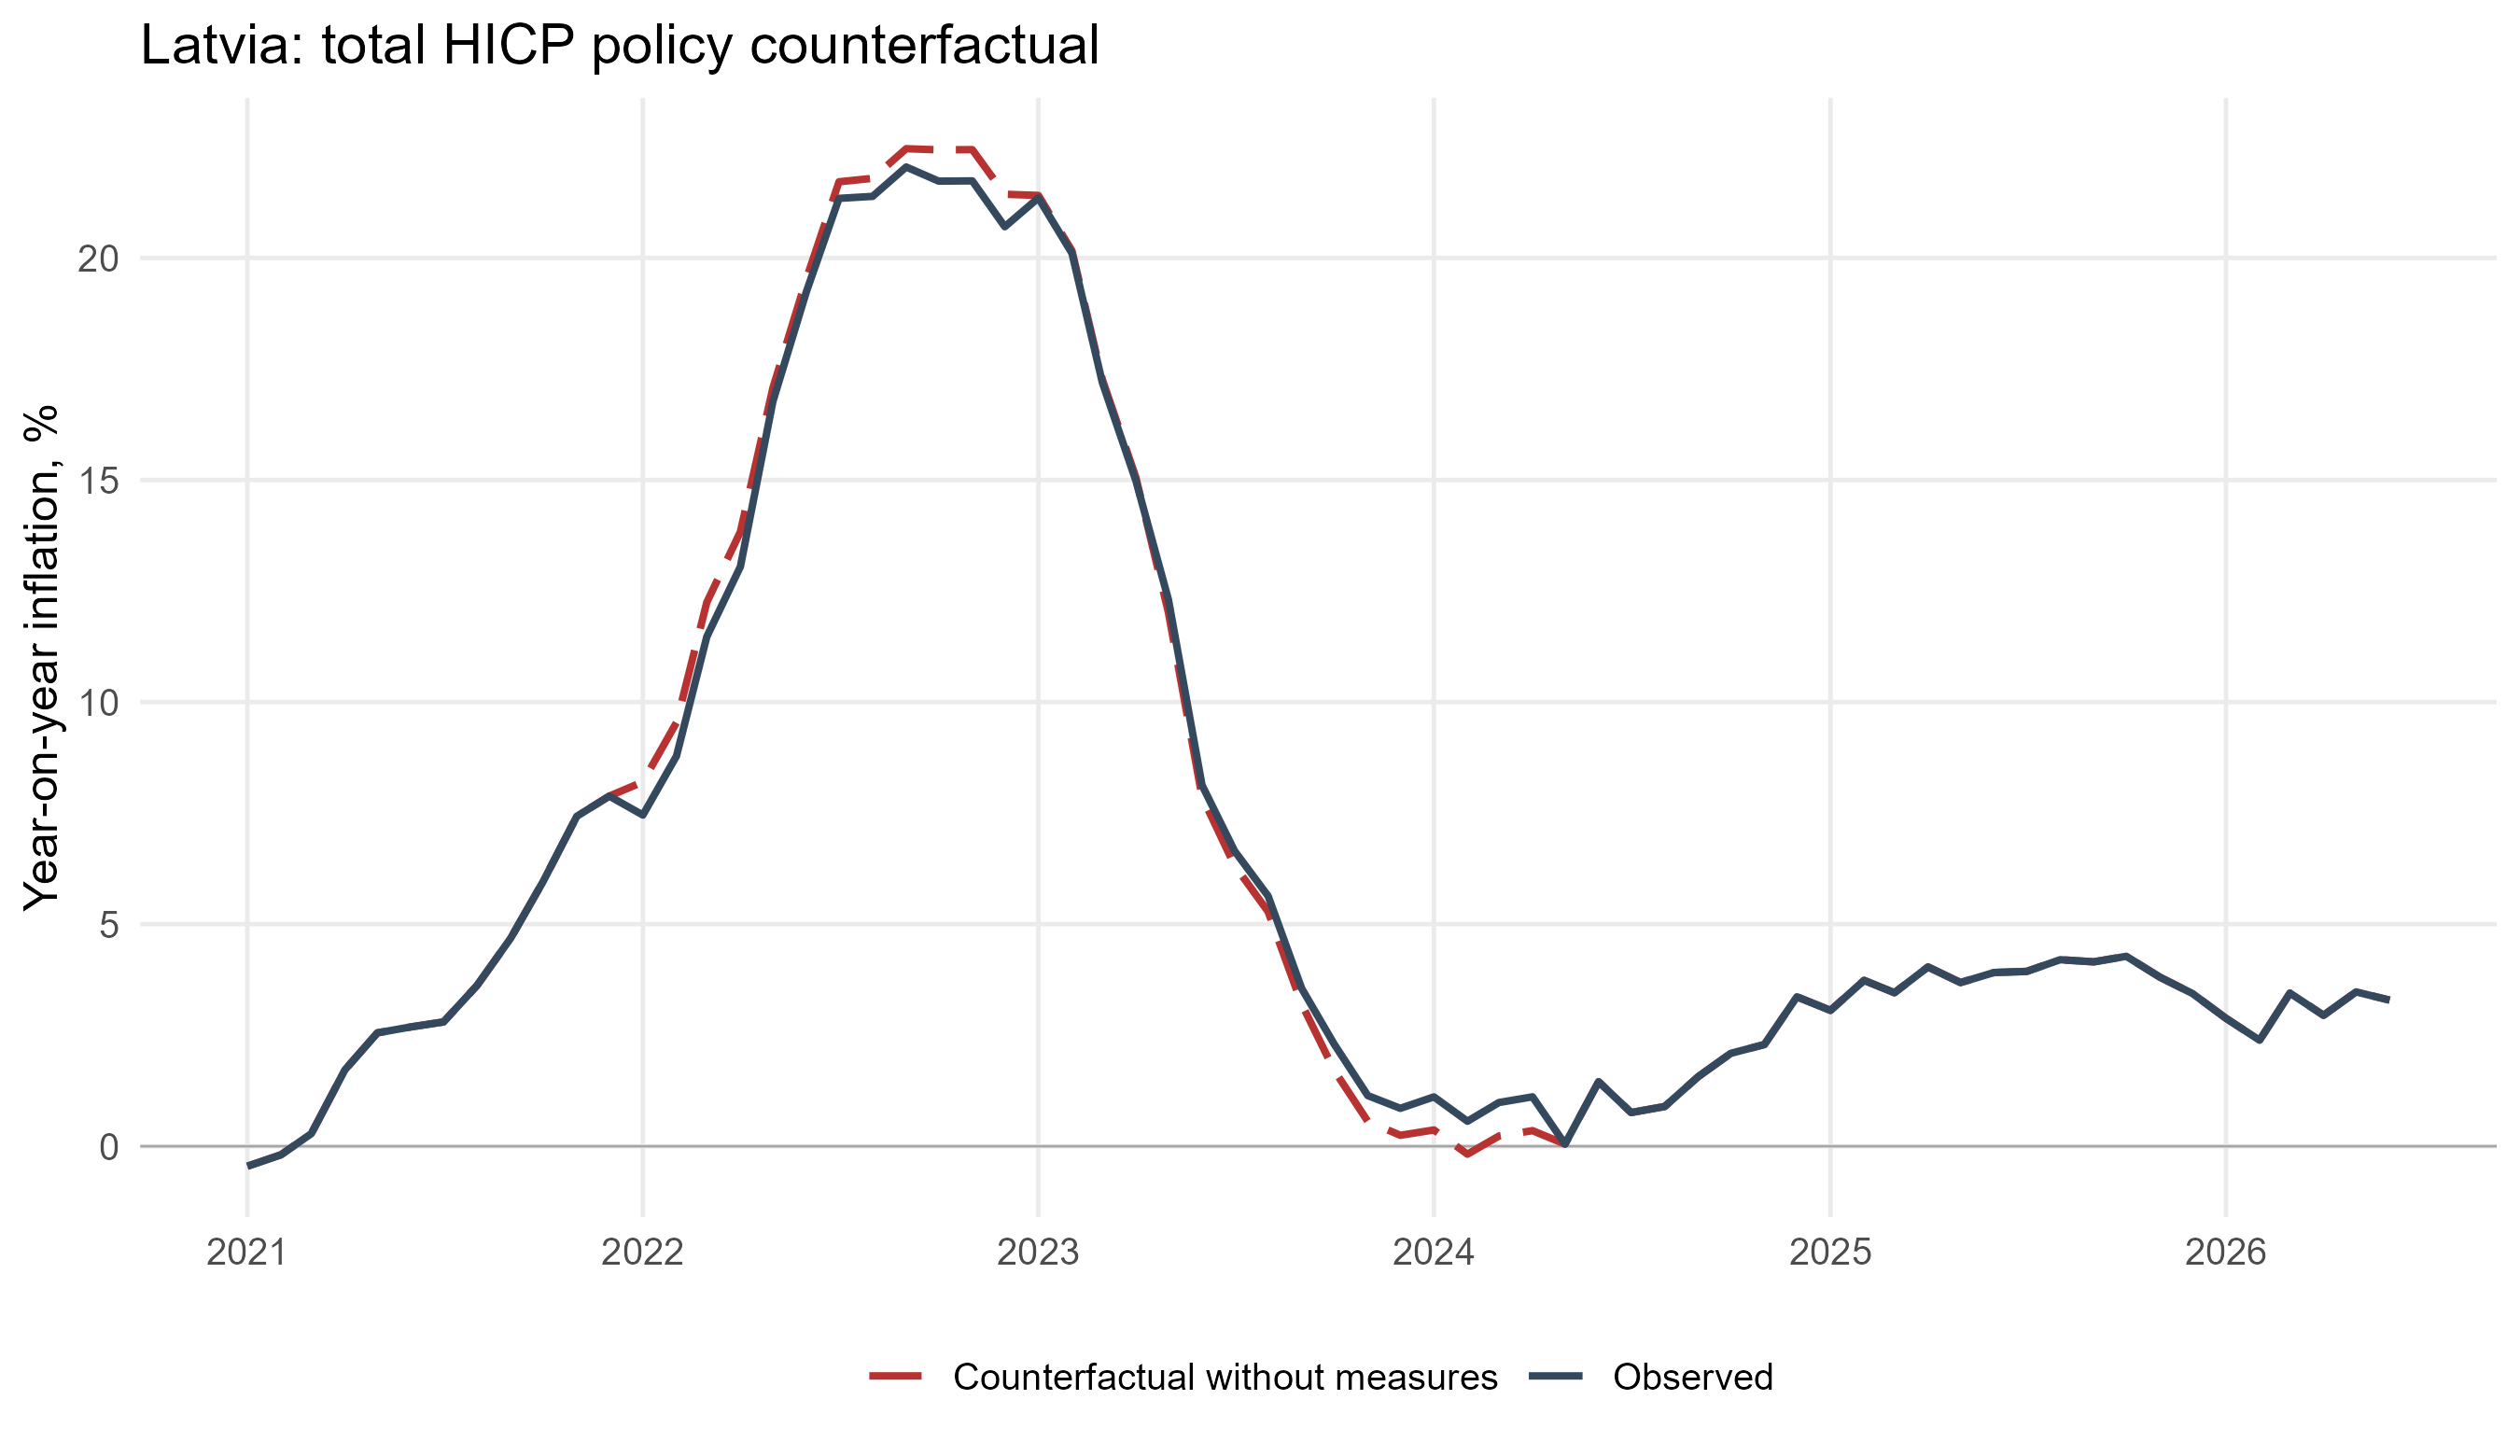
\includegraphics[width=0.86\textwidth,height=0.38\textheight,keepaspectratio]{fig/policy_total_cpi_counterfactual_inflation_LV_latvia.png}
\caption{Latvia: observed and counterfactual inflation}
\end{figure}

\subsection{Malta}
\begin{figure}[H]
\centering
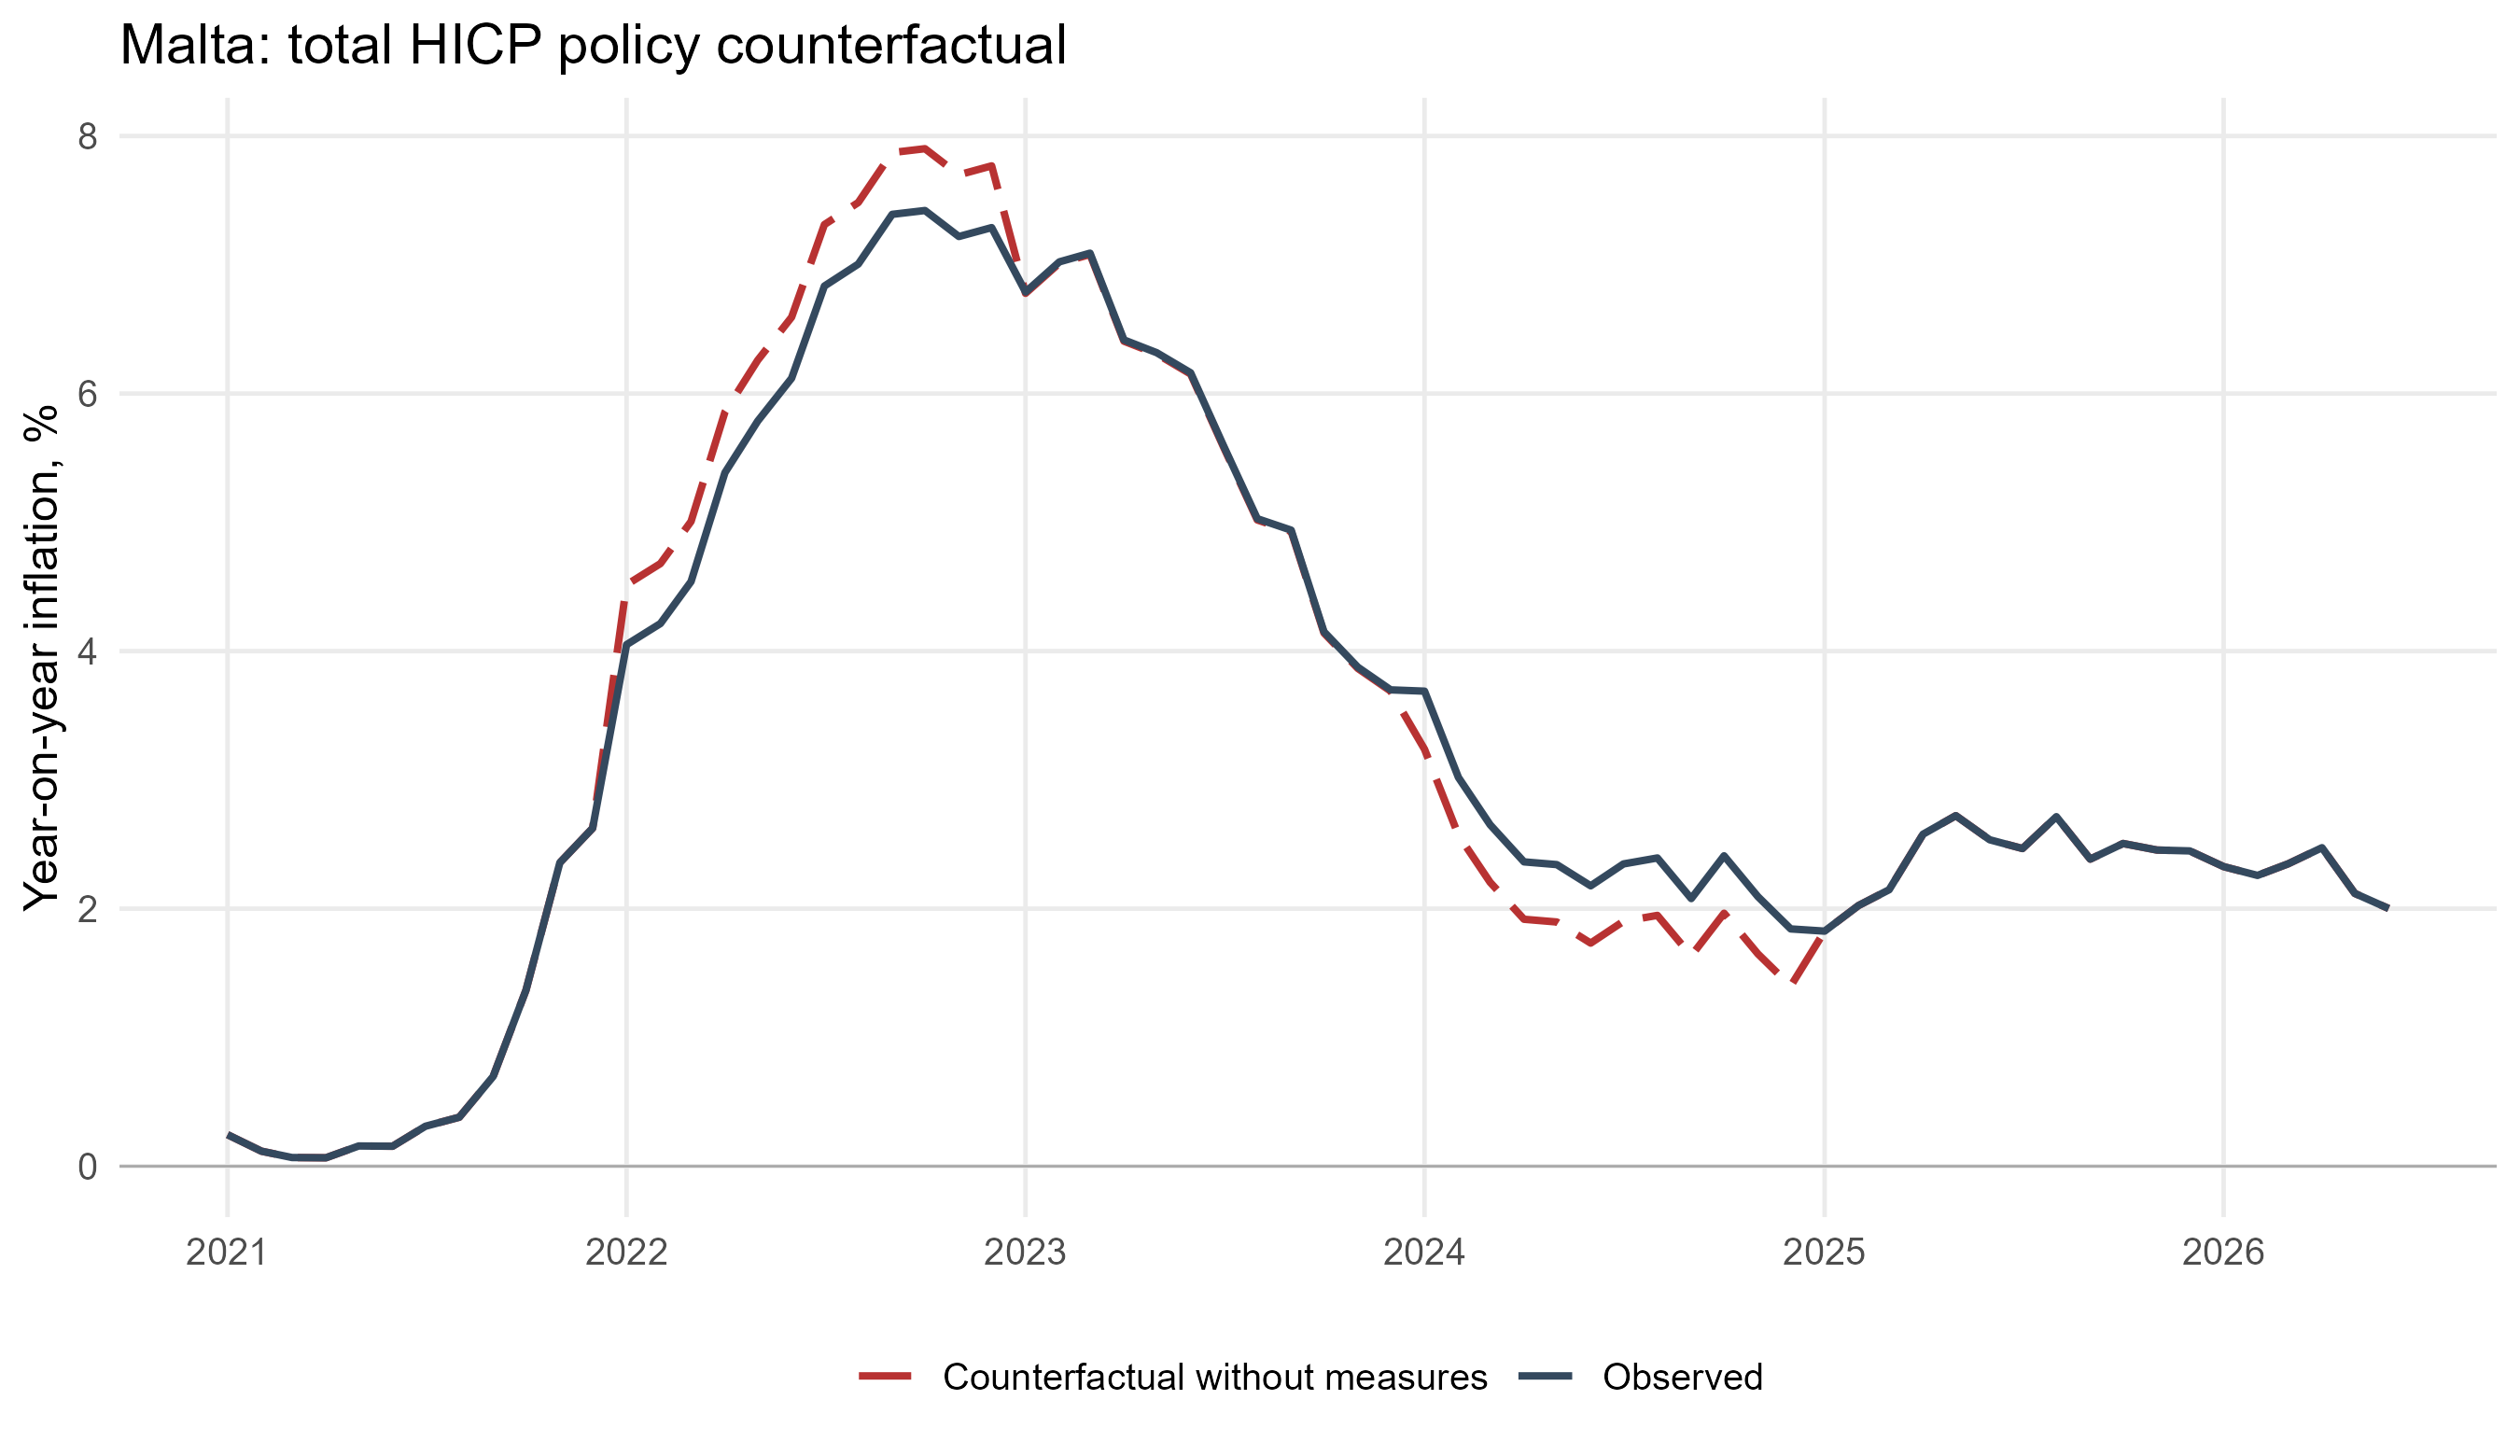
\includegraphics[width=0.86\textwidth,height=0.38\textheight,keepaspectratio]{fig/policy_total_cpi_counterfactual_inflation_MT_malta.png}
\caption{Malta: observed and counterfactual inflation}
\end{figure}

\subsection{Netherlands}
\begin{figure}[H]
\centering
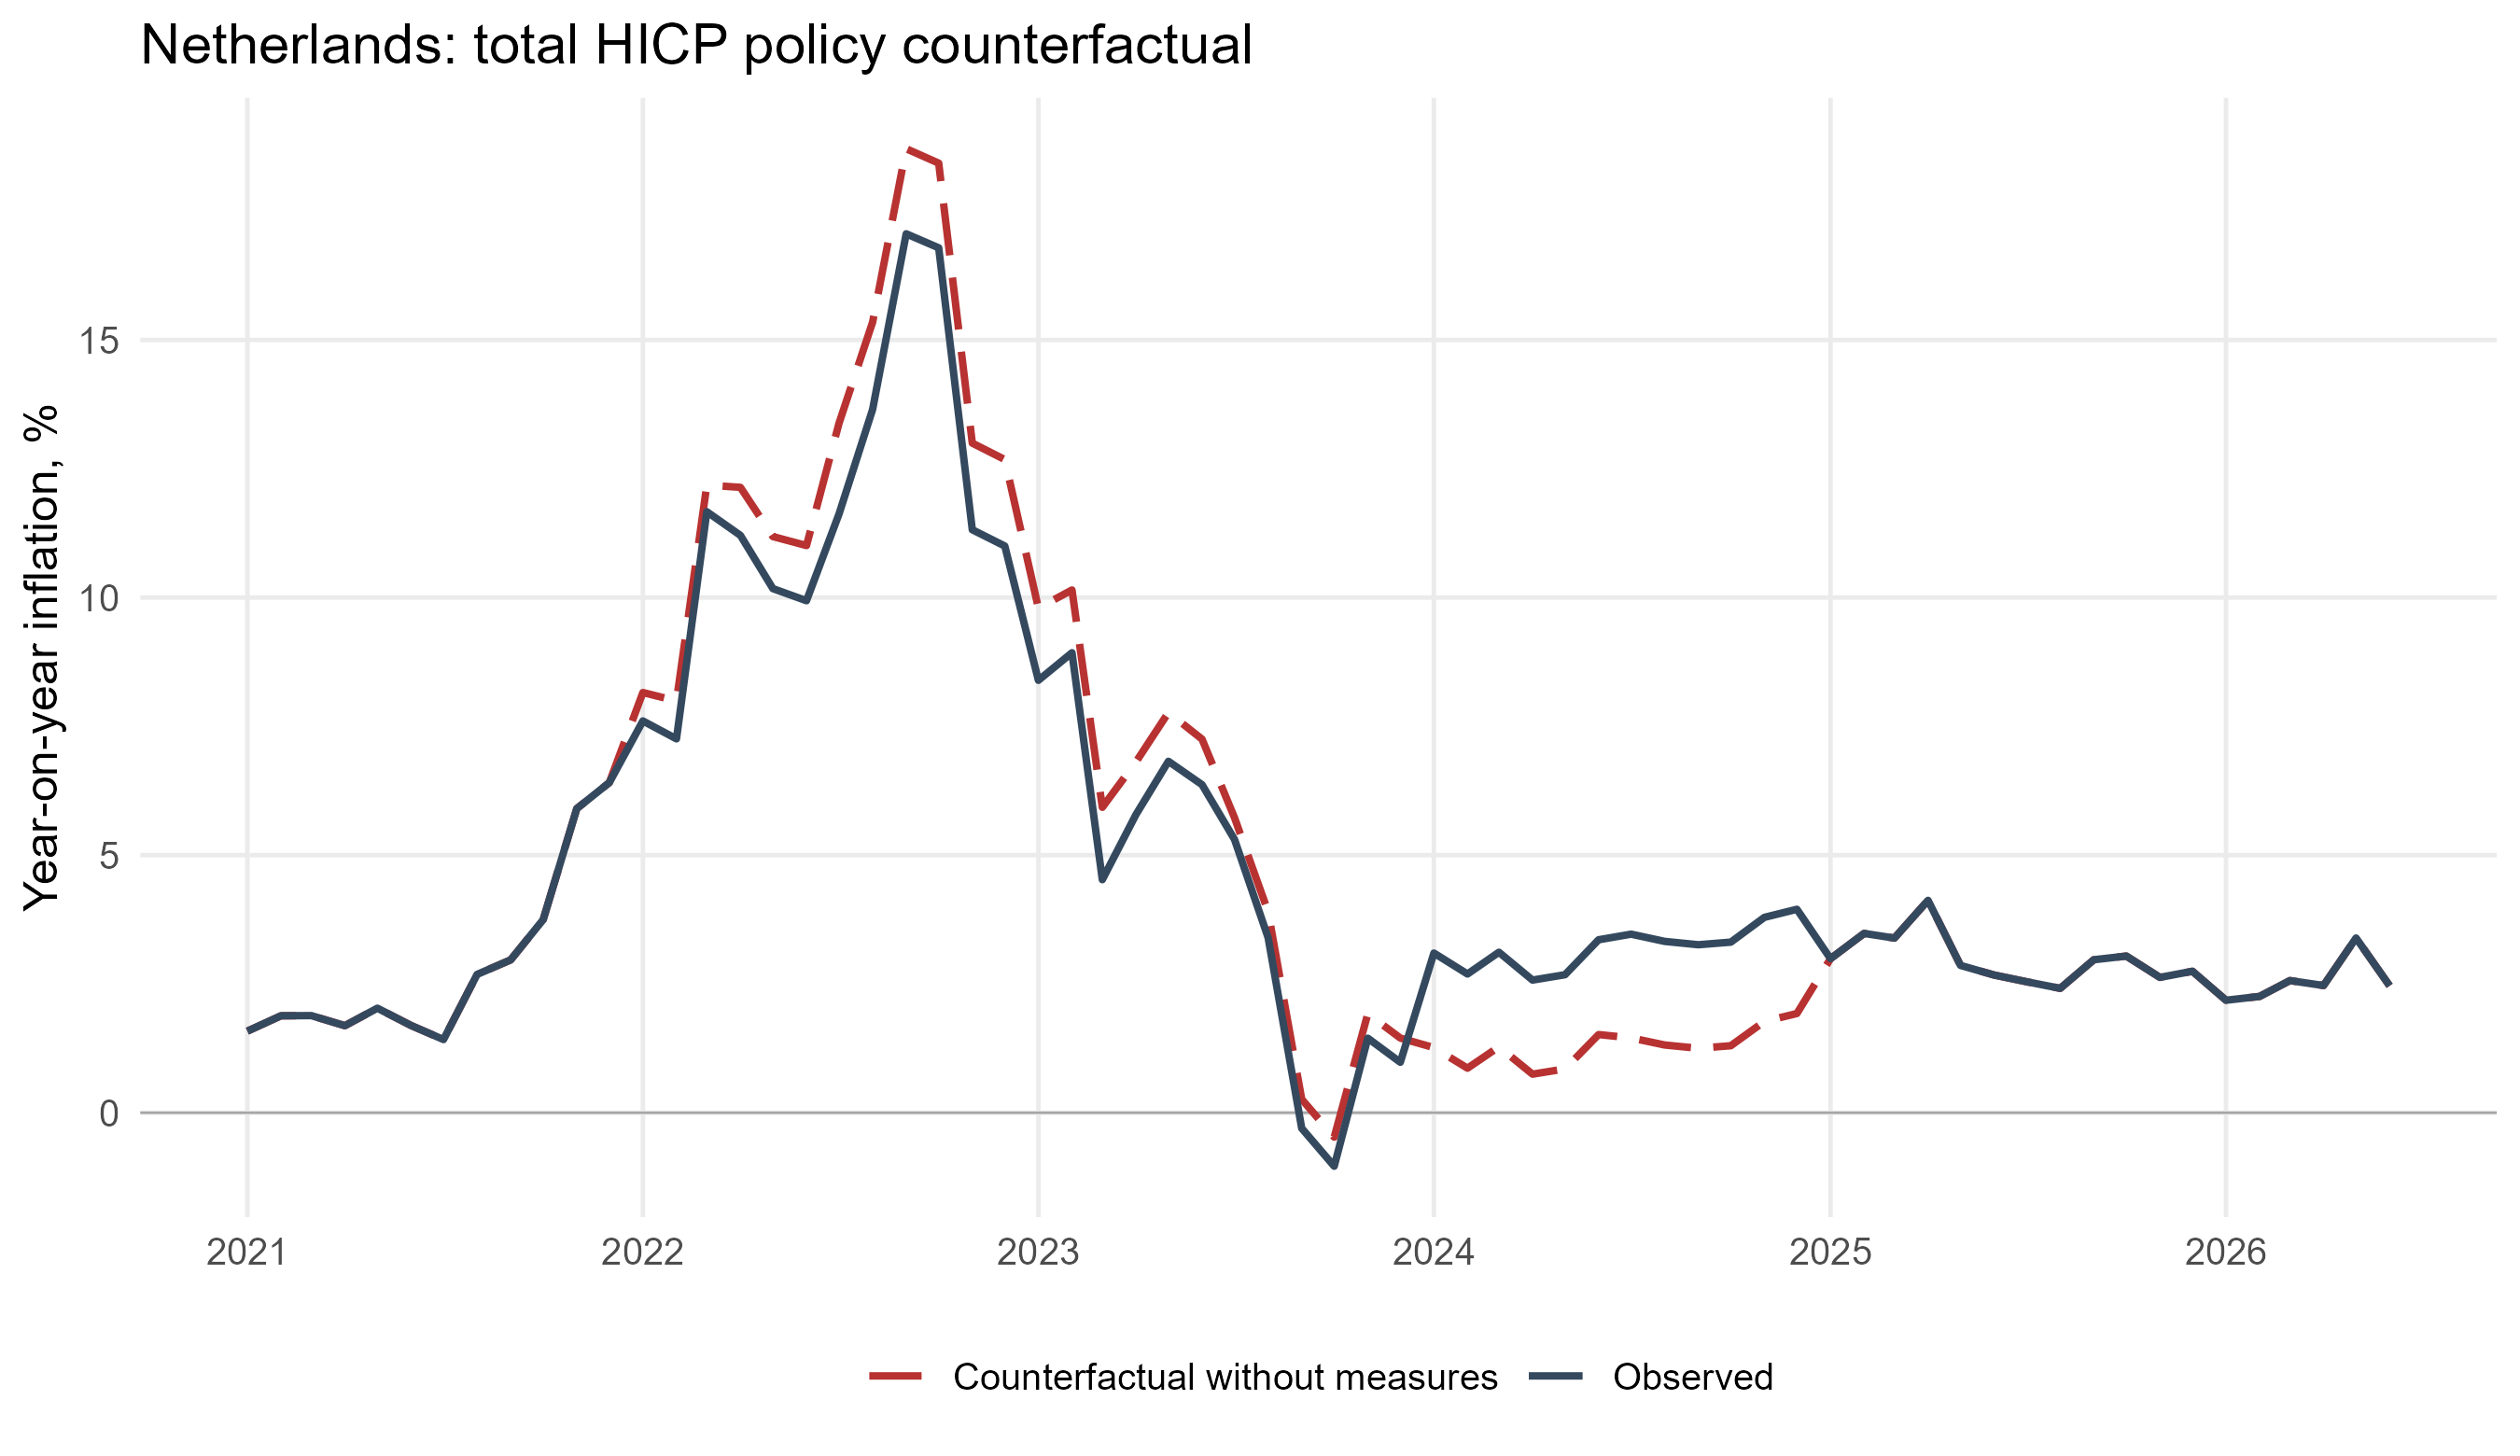
\includegraphics[width=0.86\textwidth,height=0.38\textheight,keepaspectratio]{fig/policy_total_cpi_counterfactual_inflation_NL_netherlands.png}
\caption{Netherlands: observed and counterfactual inflation}
\end{figure}

\subsection{Portugal}
\begin{figure}[H]
\centering
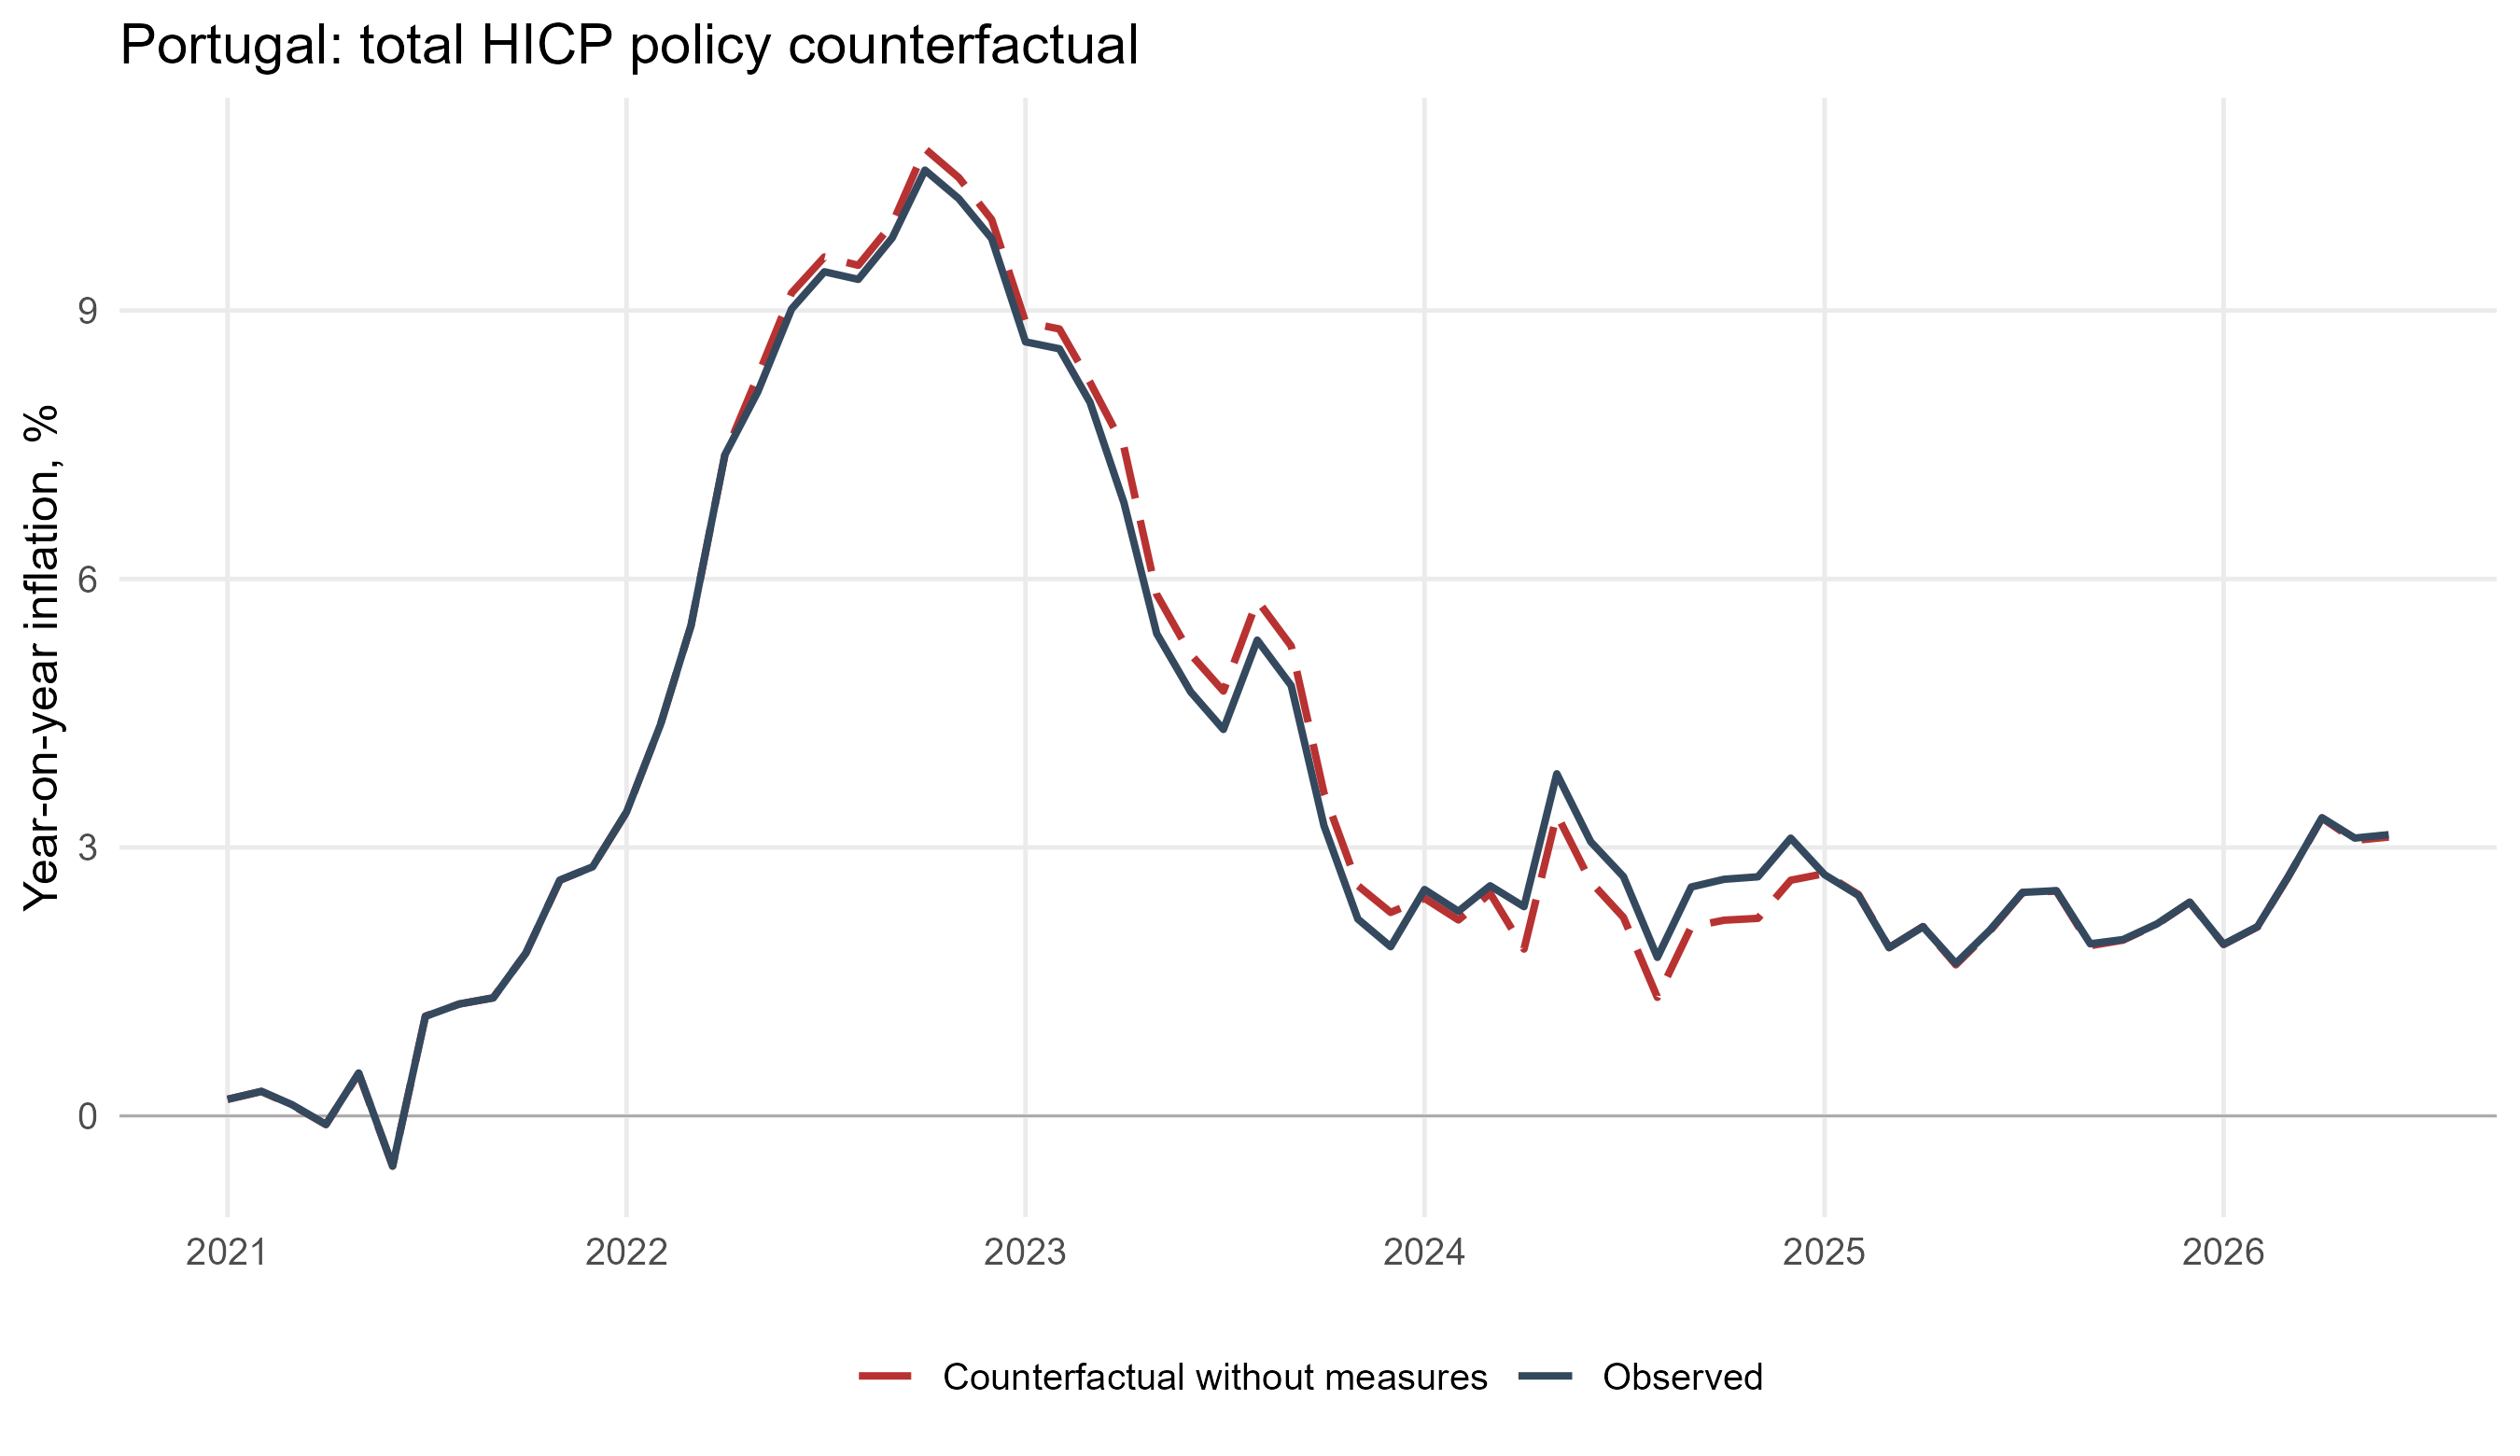
\includegraphics[width=0.86\textwidth,height=0.38\textheight,keepaspectratio]{fig/policy_total_cpi_counterfactual_inflation_PT_portugal.png}
\caption{Portugal: observed and counterfactual inflation}
\end{figure}

\subsection{Slovakia}
\begin{figure}[H]
\centering
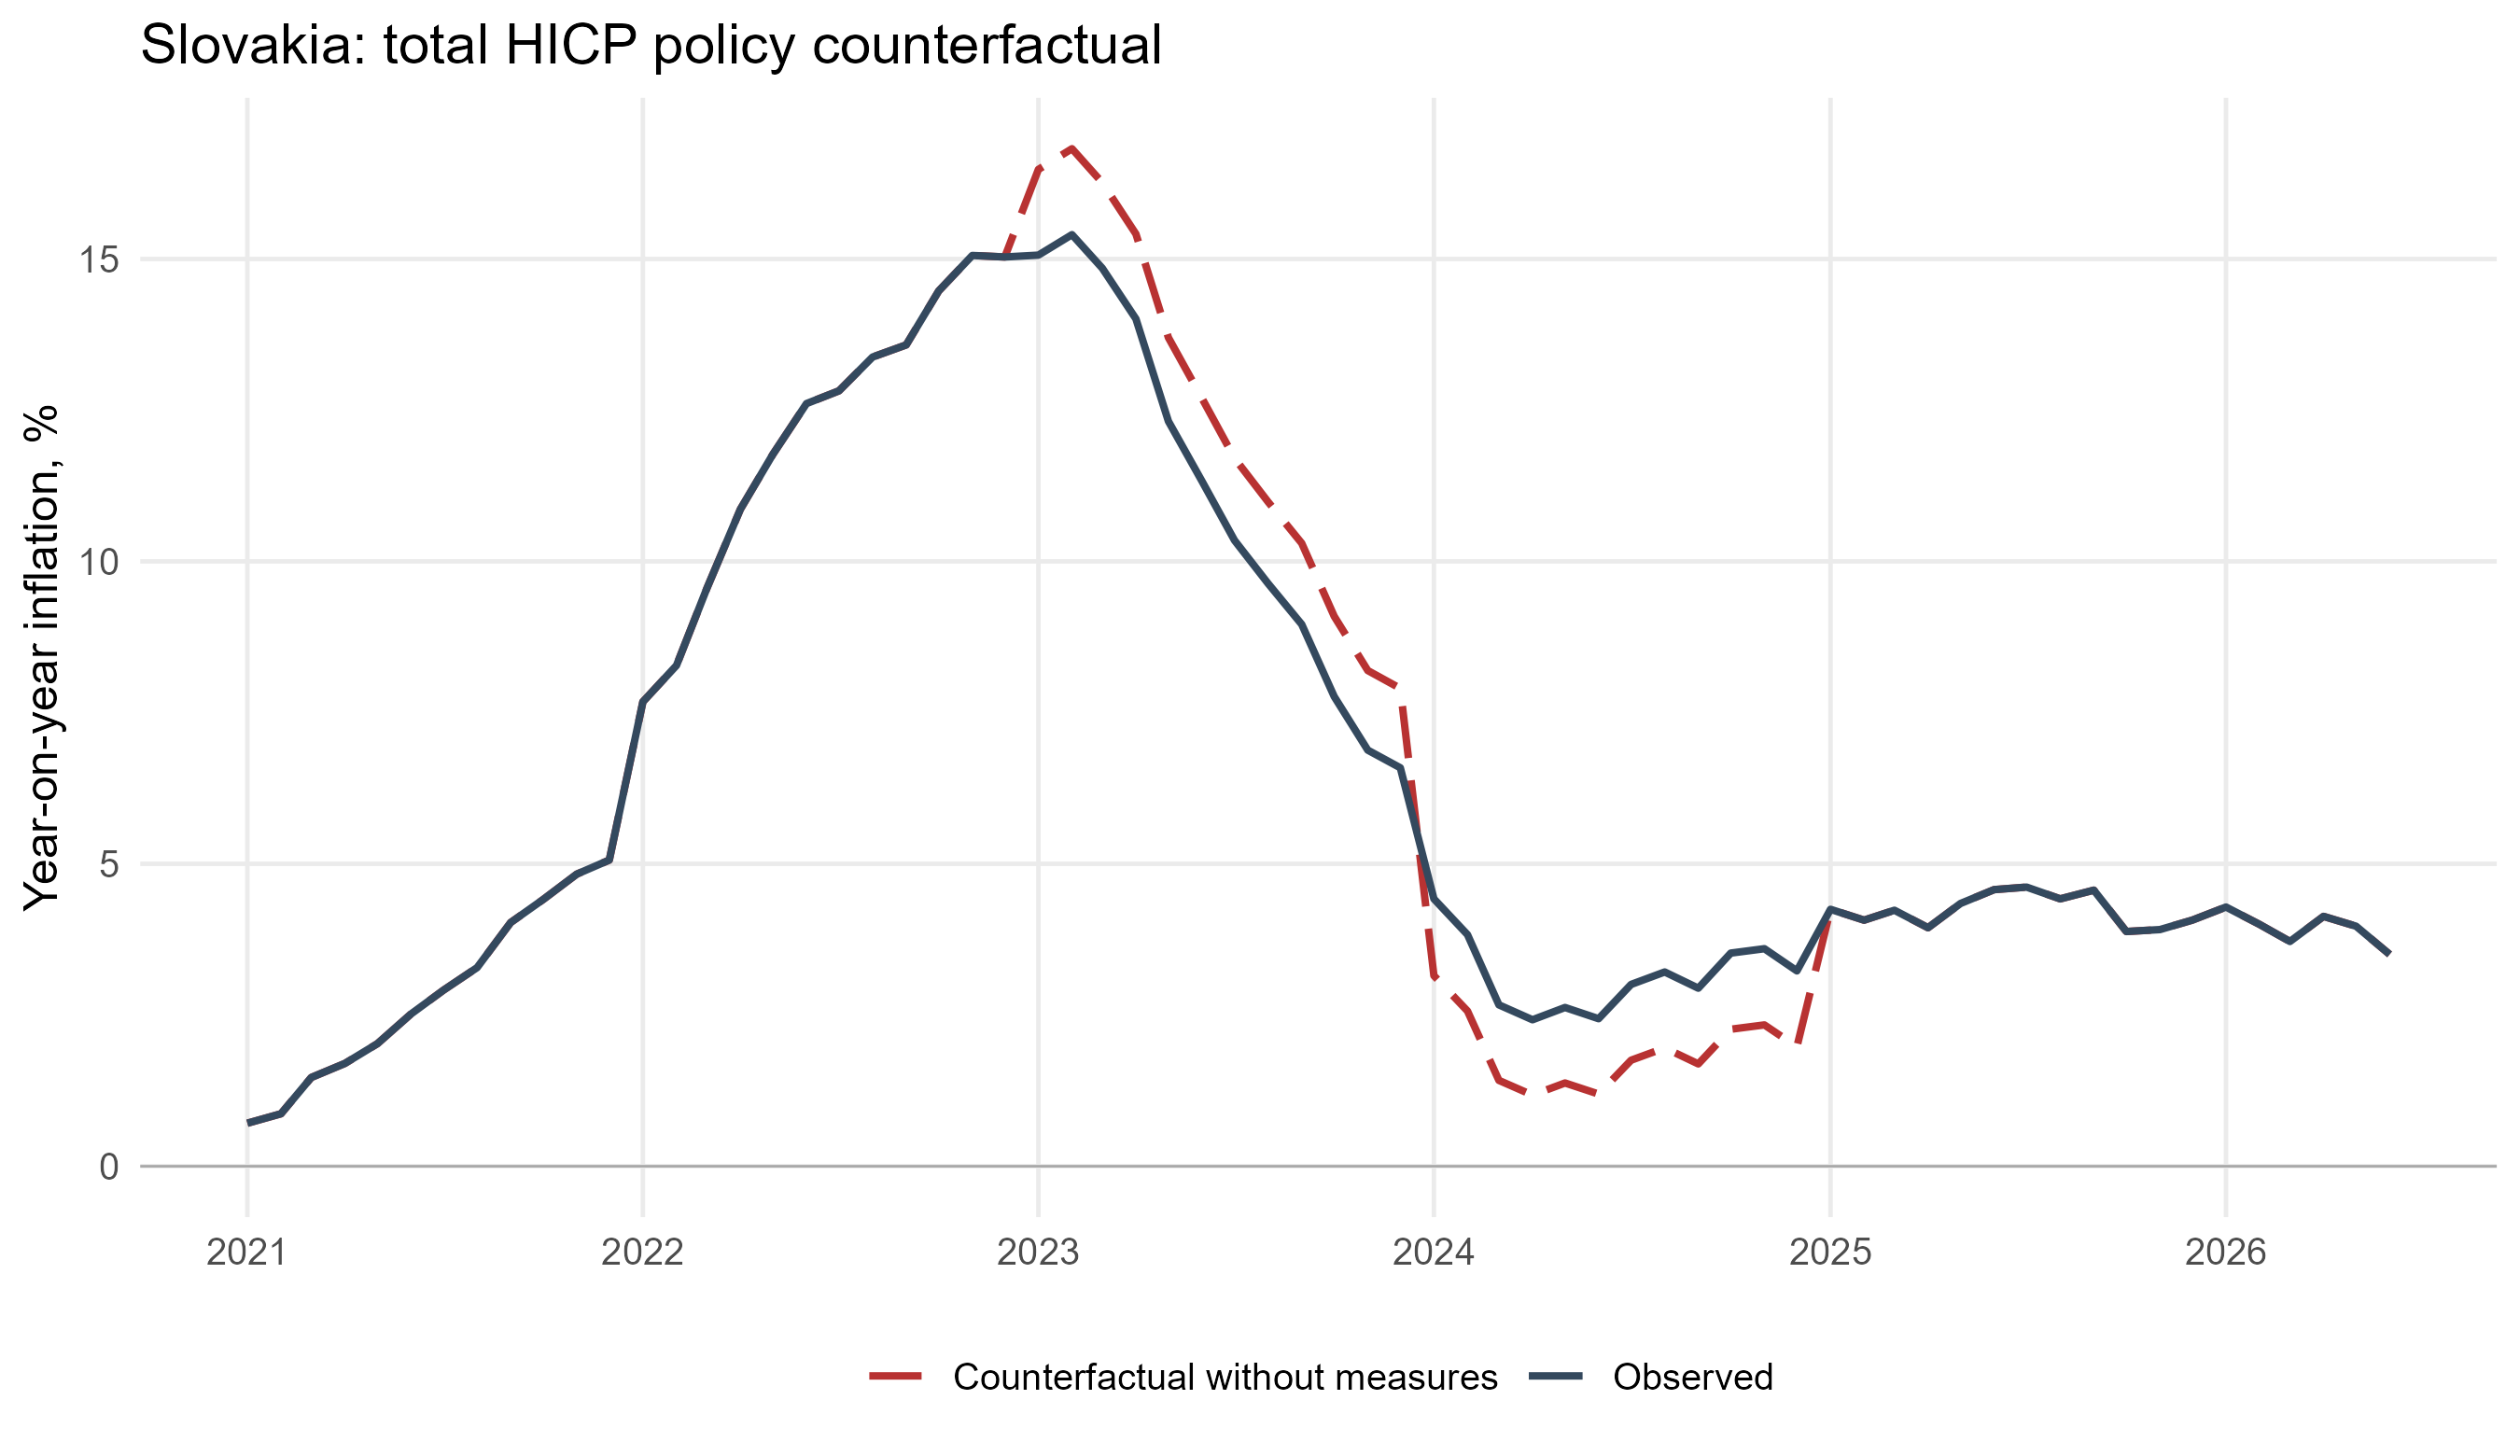
\includegraphics[width=0.86\textwidth,height=0.38\textheight,keepaspectratio]{fig/policy_total_cpi_counterfactual_inflation_SK_slovakia.png}
\caption{Slovakia: observed and counterfactual inflation}
\end{figure}

\subsection{Slovenia}
\begin{figure}[H]
\centering
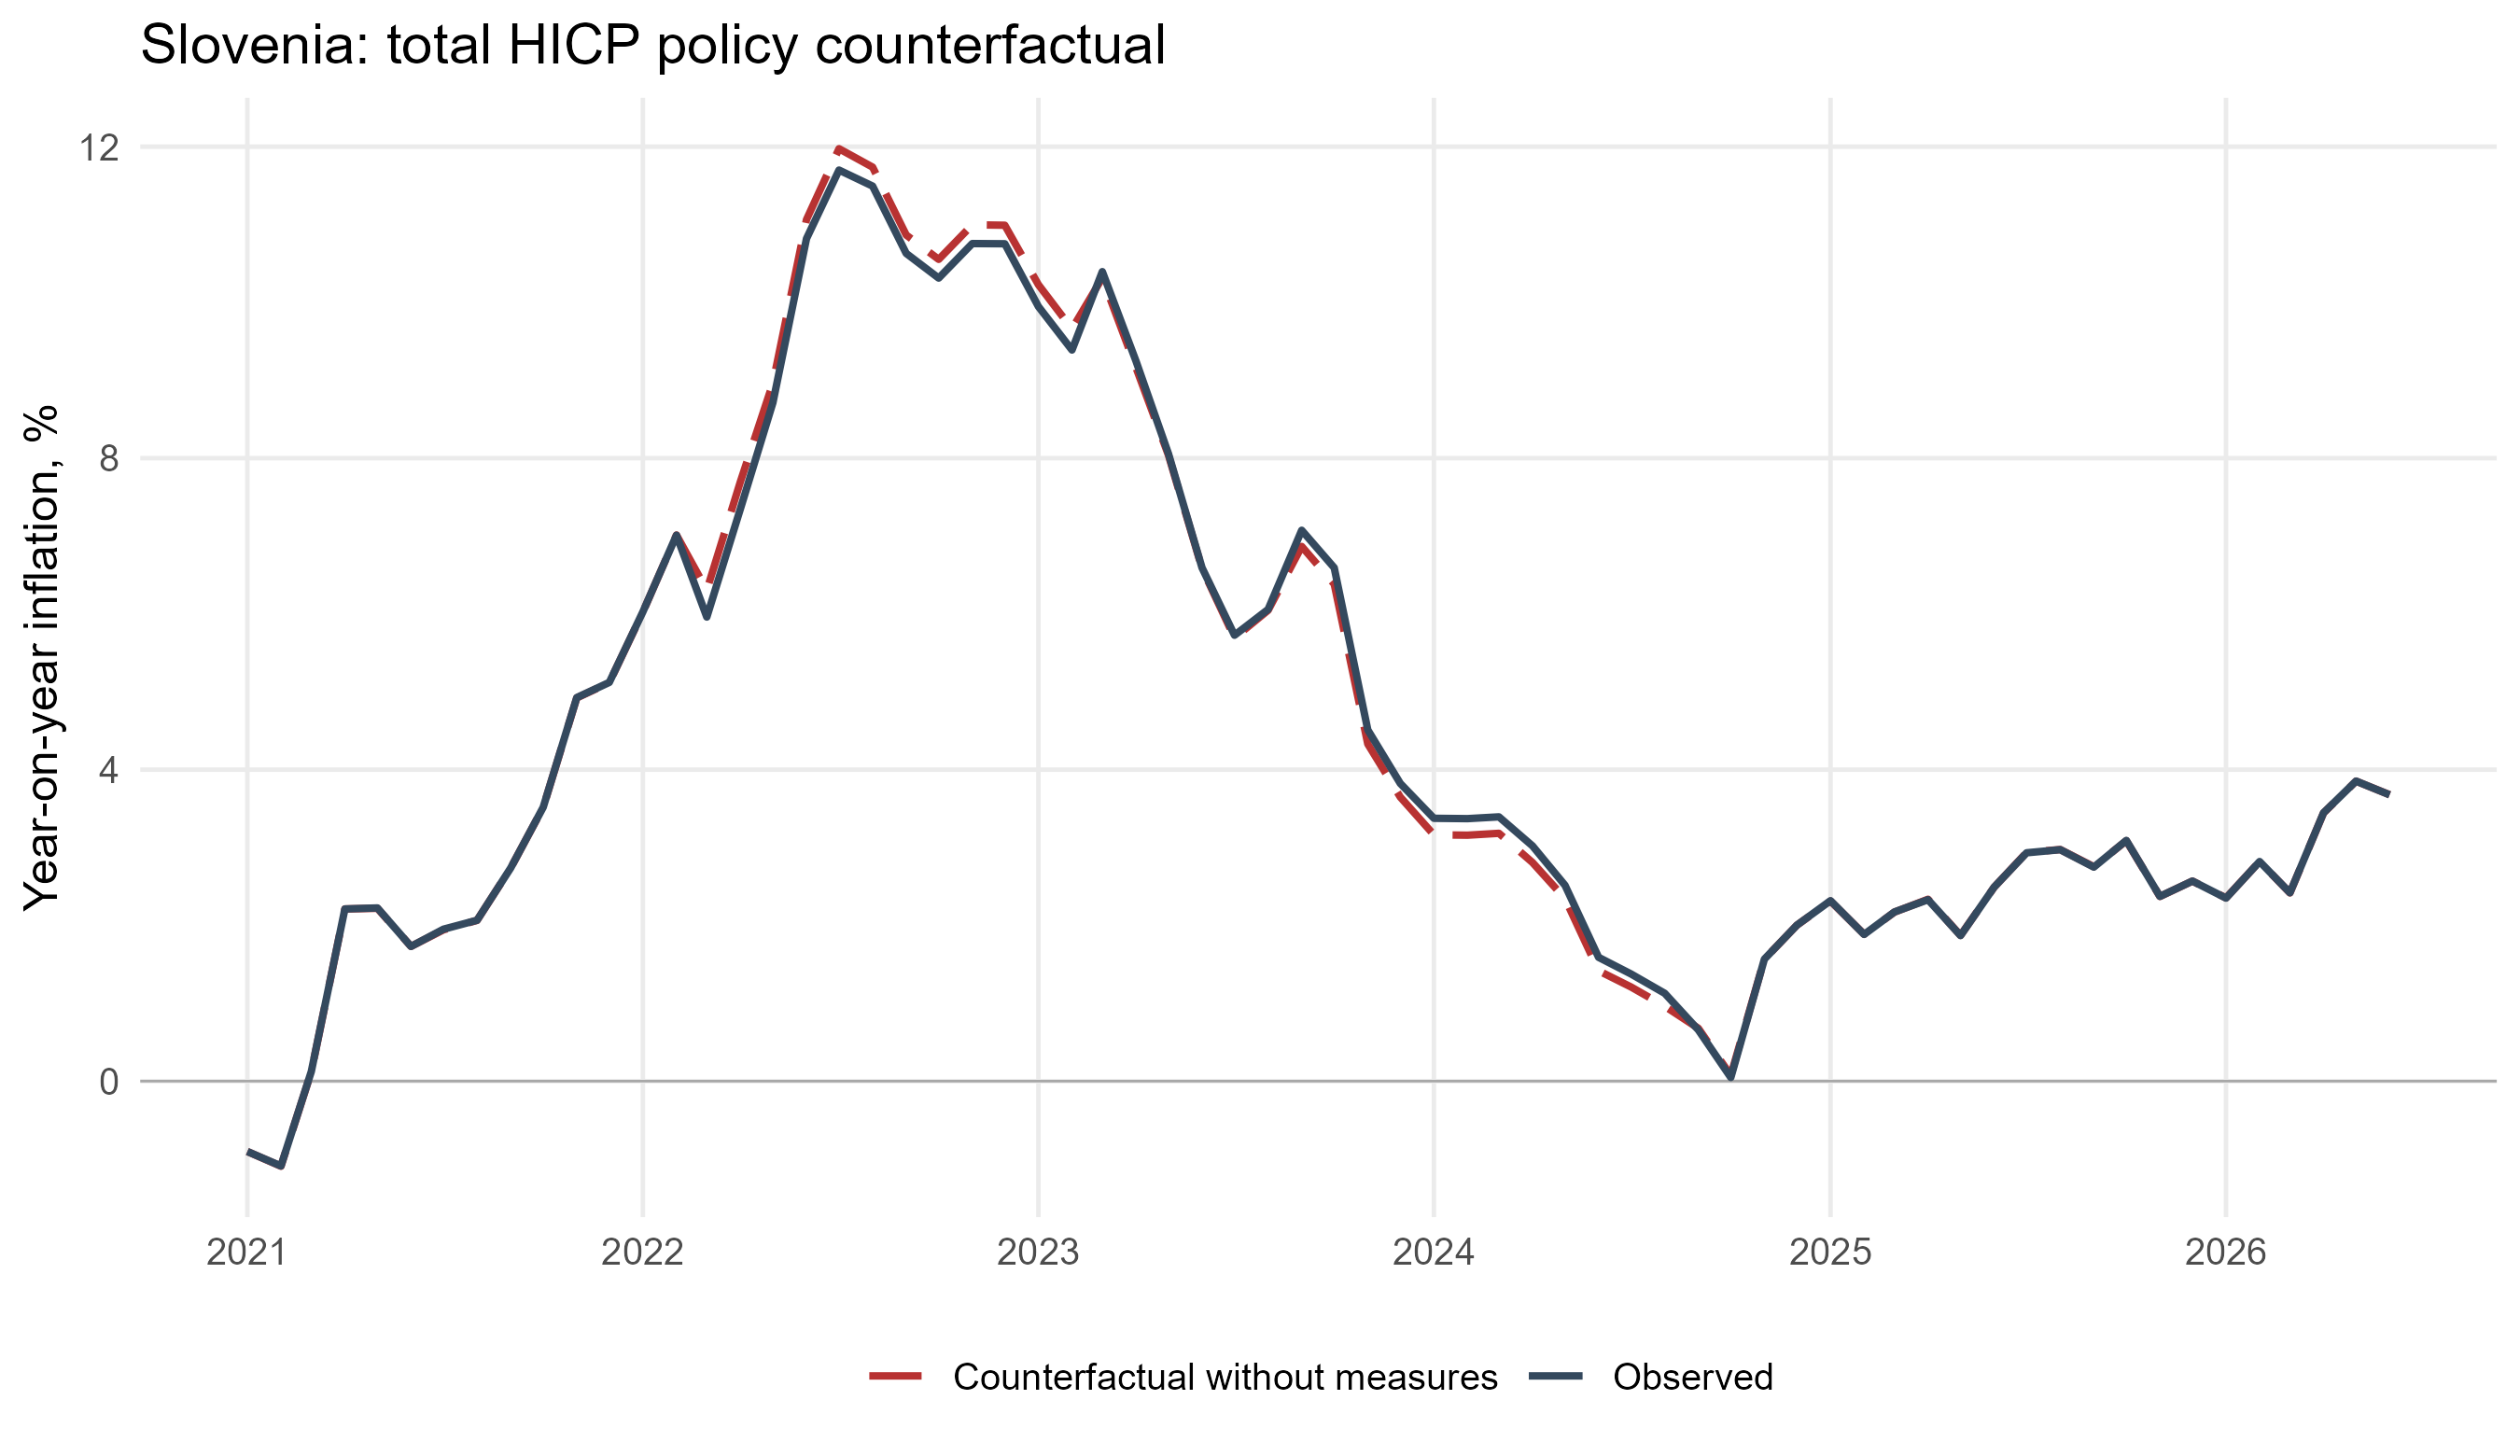
\includegraphics[width=0.86\textwidth,height=0.38\textheight,keepaspectratio]{fig/policy_total_cpi_counterfactual_inflation_SI_slovenia.png}
\caption{Slovenia: observed and counterfactual inflation}
\end{figure}



\clearpage

\section{The Household Budget Survey in Italy}
\label{sec:app-italy-hbs}

The most recent complete harmonized Eurostat HBS entry for Italy is 2005. We therefore combine it
with the 2015 and 2020 Istat public-use HBS files to construct the household-group baskets.

Age-group baskets are computed directly from the survey-weighted expenditure aggregates in the
Istat files, using the age of the household reference person.

For income quintiles, households are ranked by equivalized total consumption using the Carbonaro
scale and the survey weights. Because income quintiles are not observed in the target-year files, we
transport the relationship between income- and expenditure-quintile baskets observed in 2005. Let
$E_{jqy}$ denote expenditure on COICOP group $j$ by expenditure quintile $q$ in year $y$, and let
$s^{I}_{jq,2005}$ and $s^{E}_{jq,2005}$ denote the corresponding 2005 shares for income and
expenditure quintiles. The estimated income-quintile consumption structure is

\begin{equation}
\widehat{s}^{I}_{jqy}
=
\frac{E_{jqy}\left(s^{I}_{jq,2005}/s^{E}_{jq,2005}\right)}
{\sum_k E_{kqy}\left(s^{I}_{kq,2005}/s^{E}_{kq,2005}\right)}.
\label{eq:italy-income-expenditure-bridge}
\end{equation}

Thus, the 2005 income-to-expenditure ratio adjusts each 2015 or 2020 expenditure-quintile component,
after which the basket is renormalized to one. A few broad groups are combined to reconcile the two
2005 classifications. The resulting income-quintile structures are estimated rather than directly
observed. The procedure addresses the same
absence of jointly observed income and consumption discussed by \citet{donatiello2022joint}.

Table~\ref{tab:it-hbs-all-products} reports the resulting shares of total consumption. Age shares are
direct survey estimates; income-quintile shares are bridge estimates. The first and fifth income
quintiles account for about 8 and 39 percent of Italian consumption, respectively.

\clearpage

\input{tables/tab_IT_hbs_all_products_by_group}

\newpage
\setcounter{figure}{2}

\begin{figure}[H]
\centering
\caption{Price indices by household group, Italy, COICOP digit 3 (index, 1996 = 100)}
\label{fig:app-it-level2-price-indices}
\begin{subfigure}{0.98\textwidth}
  \centering
  \caption{Income quintiles}
  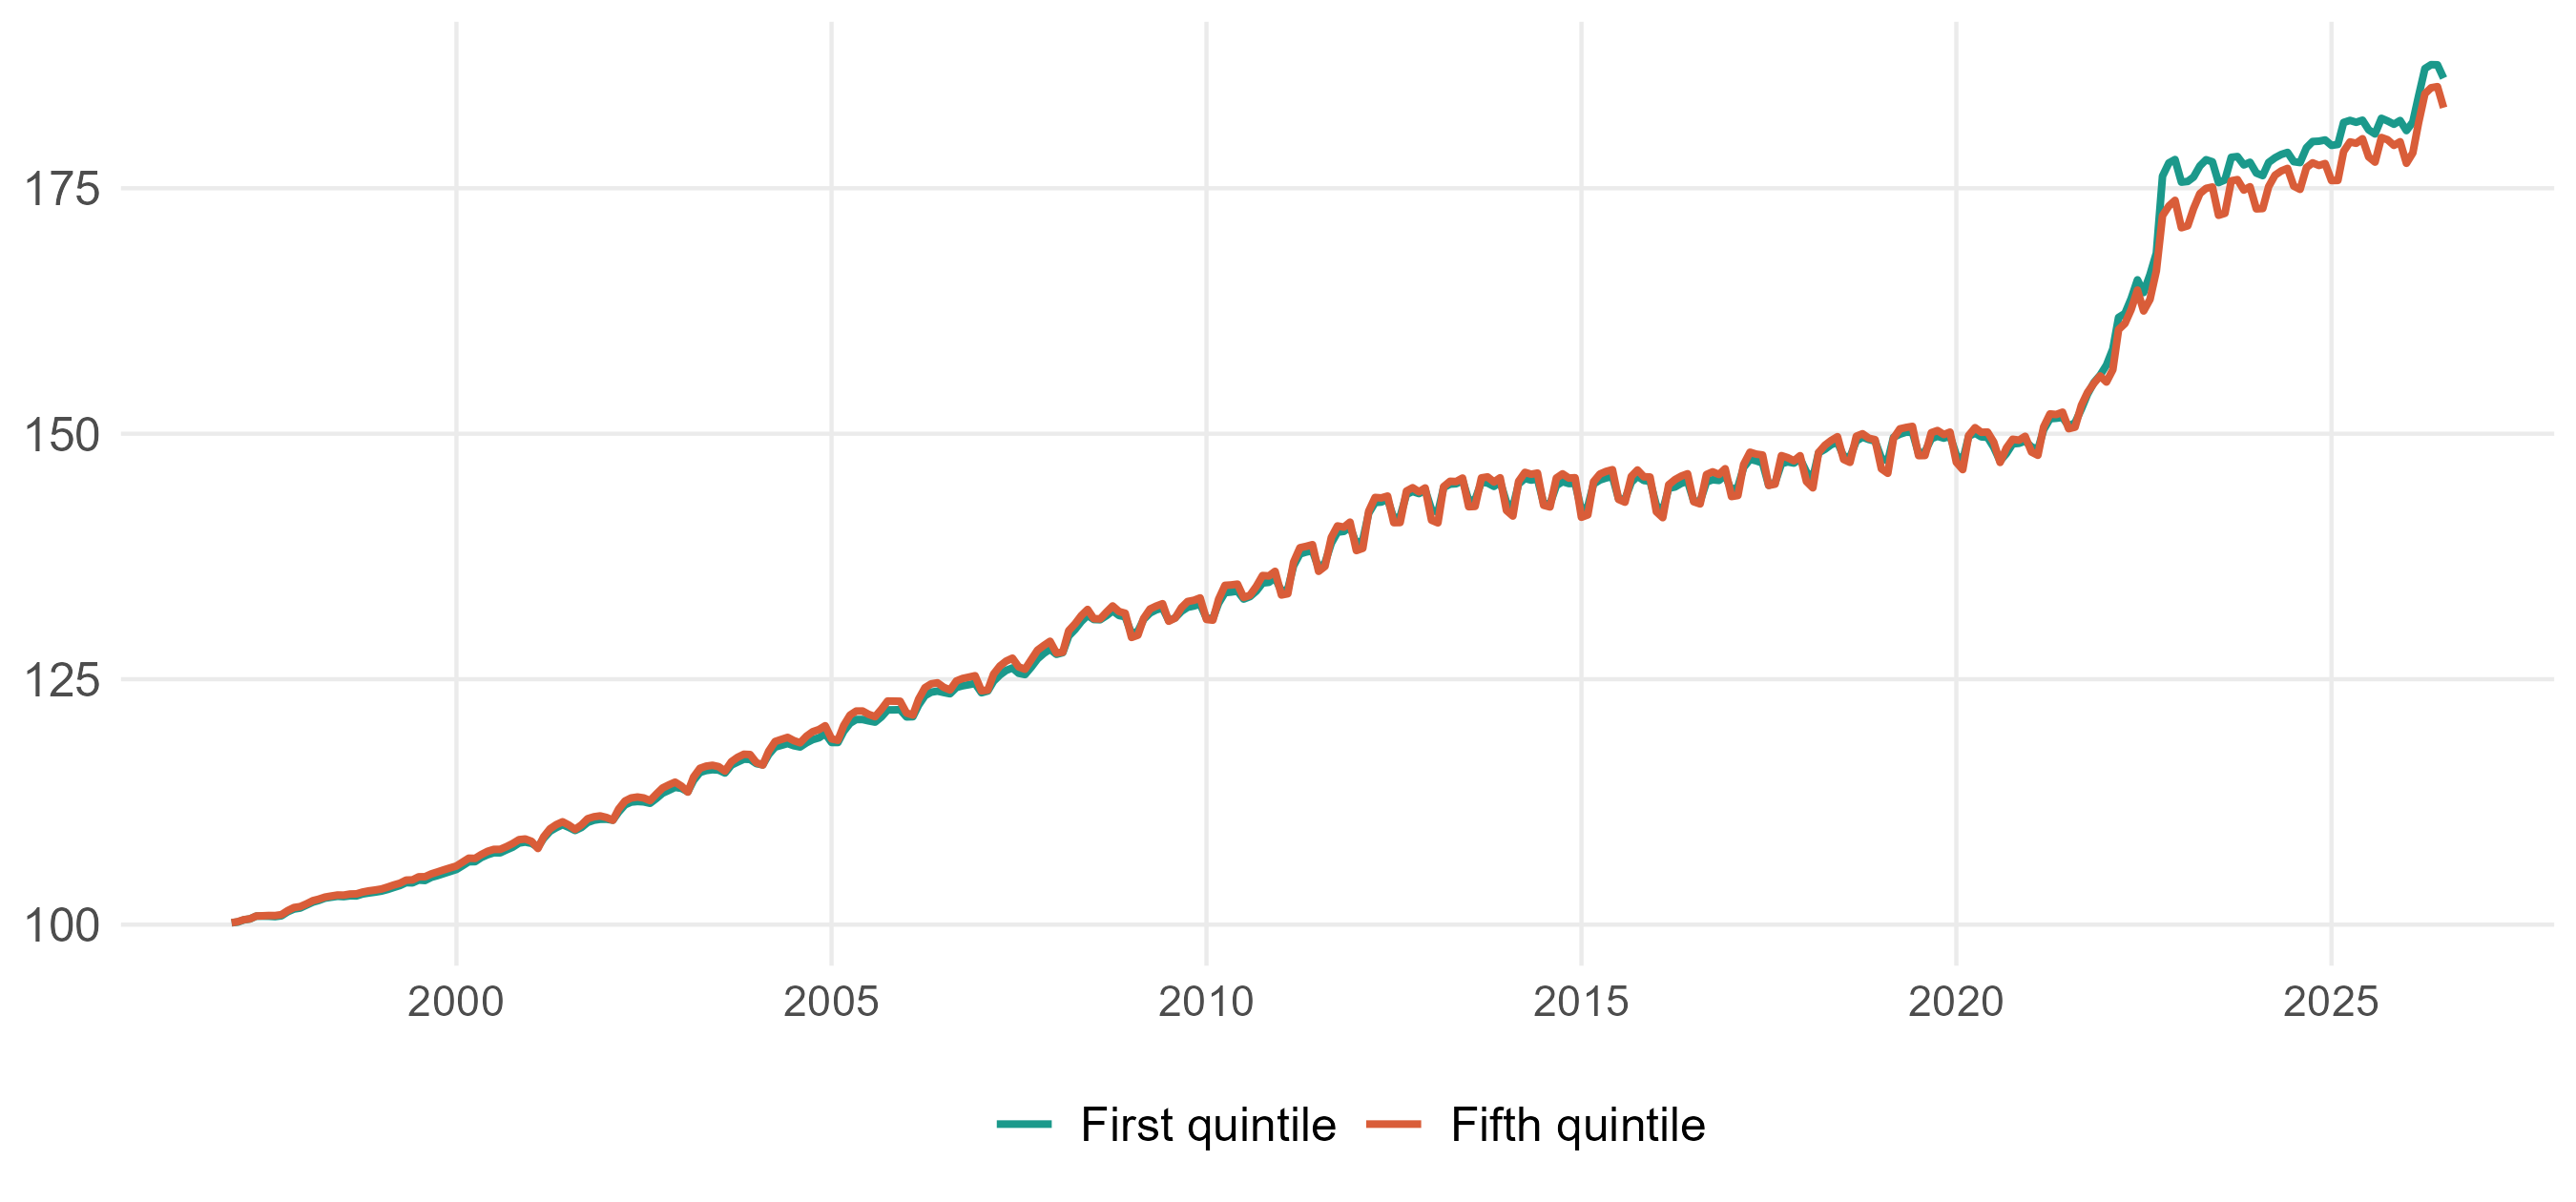
\includegraphics[width=\linewidth,height=0.32\textheight,keepaspectratio]{fig/fig_IT_1996_2026_income_price_index_level2_Q1_Q5.png}
\end{subfigure}
\vspace{6pt}
\begin{subfigure}{0.98\textwidth}
  \centering
  \caption{Age groups}
  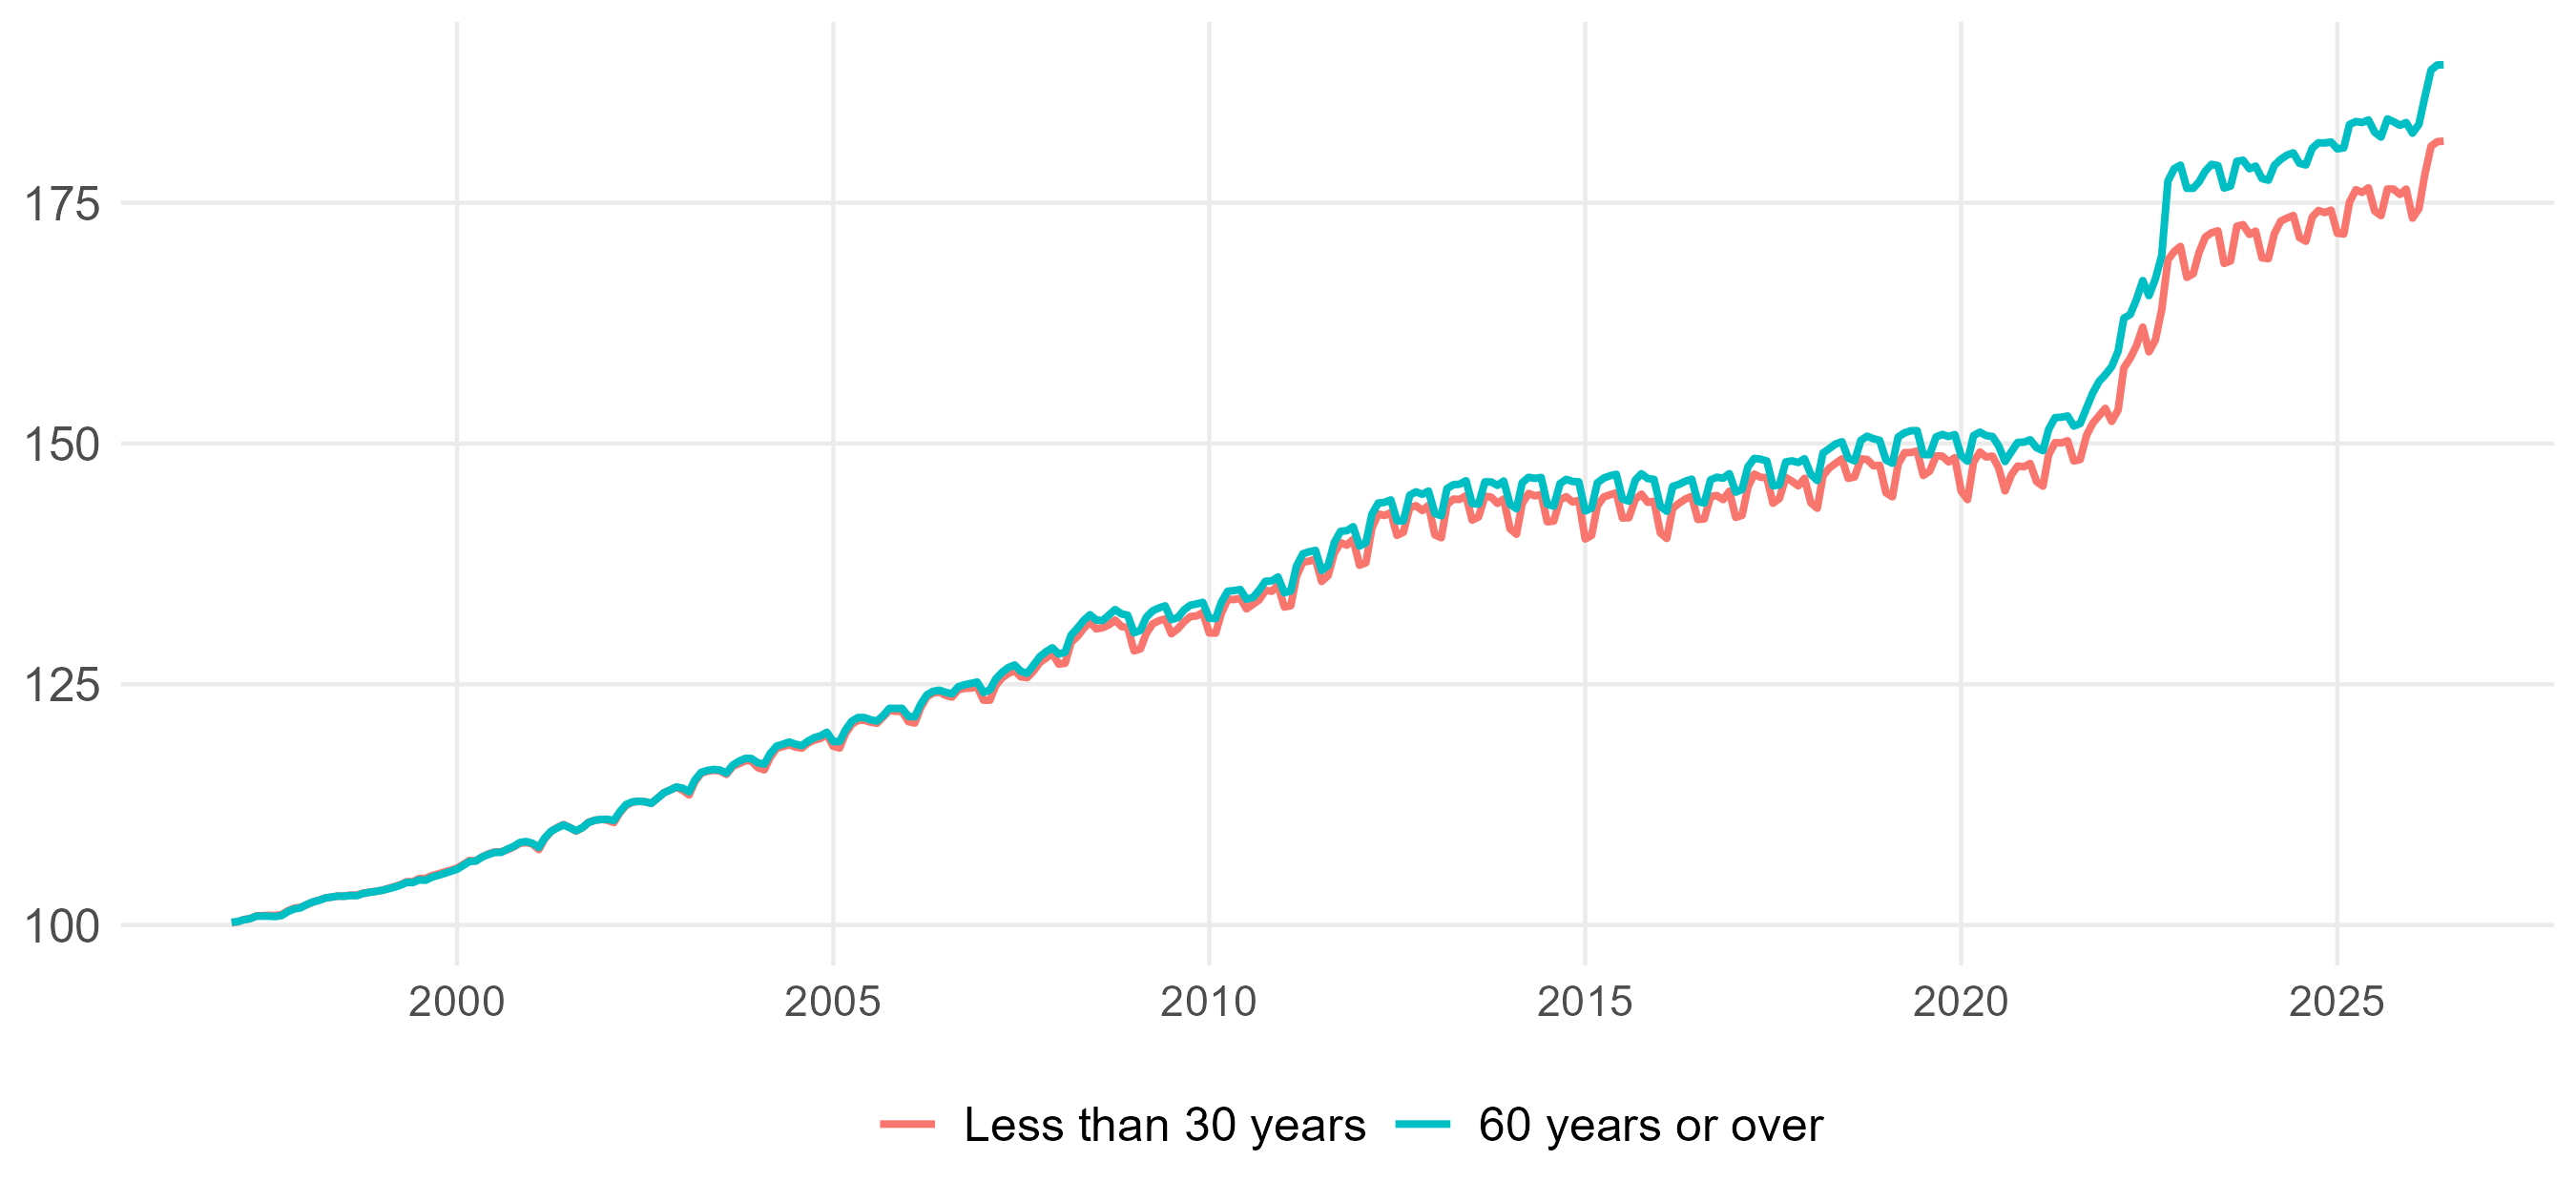
\includegraphics[width=\linewidth,height=0.32\textheight,keepaspectratio]{fig/fig_IT_1996_2026_age_price_index_level2_young_old.png}
\end{subfigure}
\vspace{8pt}
\captionsetup{font=footnotesize, format=hang, singlelinecheck=false, justification=justified}
\caption*{Notes: The figure reports chained price indices using RAS weighting. Income groups compare the first and fifth quintiles; age groups compare households whose reference person is under 30 with those aged 60 or over.\\
Sources: Eurostat HICP; Italian HBS inputs described in Appendix~\ref{sec:app-italy-hbs}; authors' calculations.}
\end{figure}
\newpage

\begin{figure}[H]
\centering
\caption{Inflation by household group, Italy, COICOP digit 3 (in \%)}
\label{fig:app-it-level2-inflation}
\begin{subfigure}{0.88\textwidth}
  \centering
  \caption{Income quintiles}
  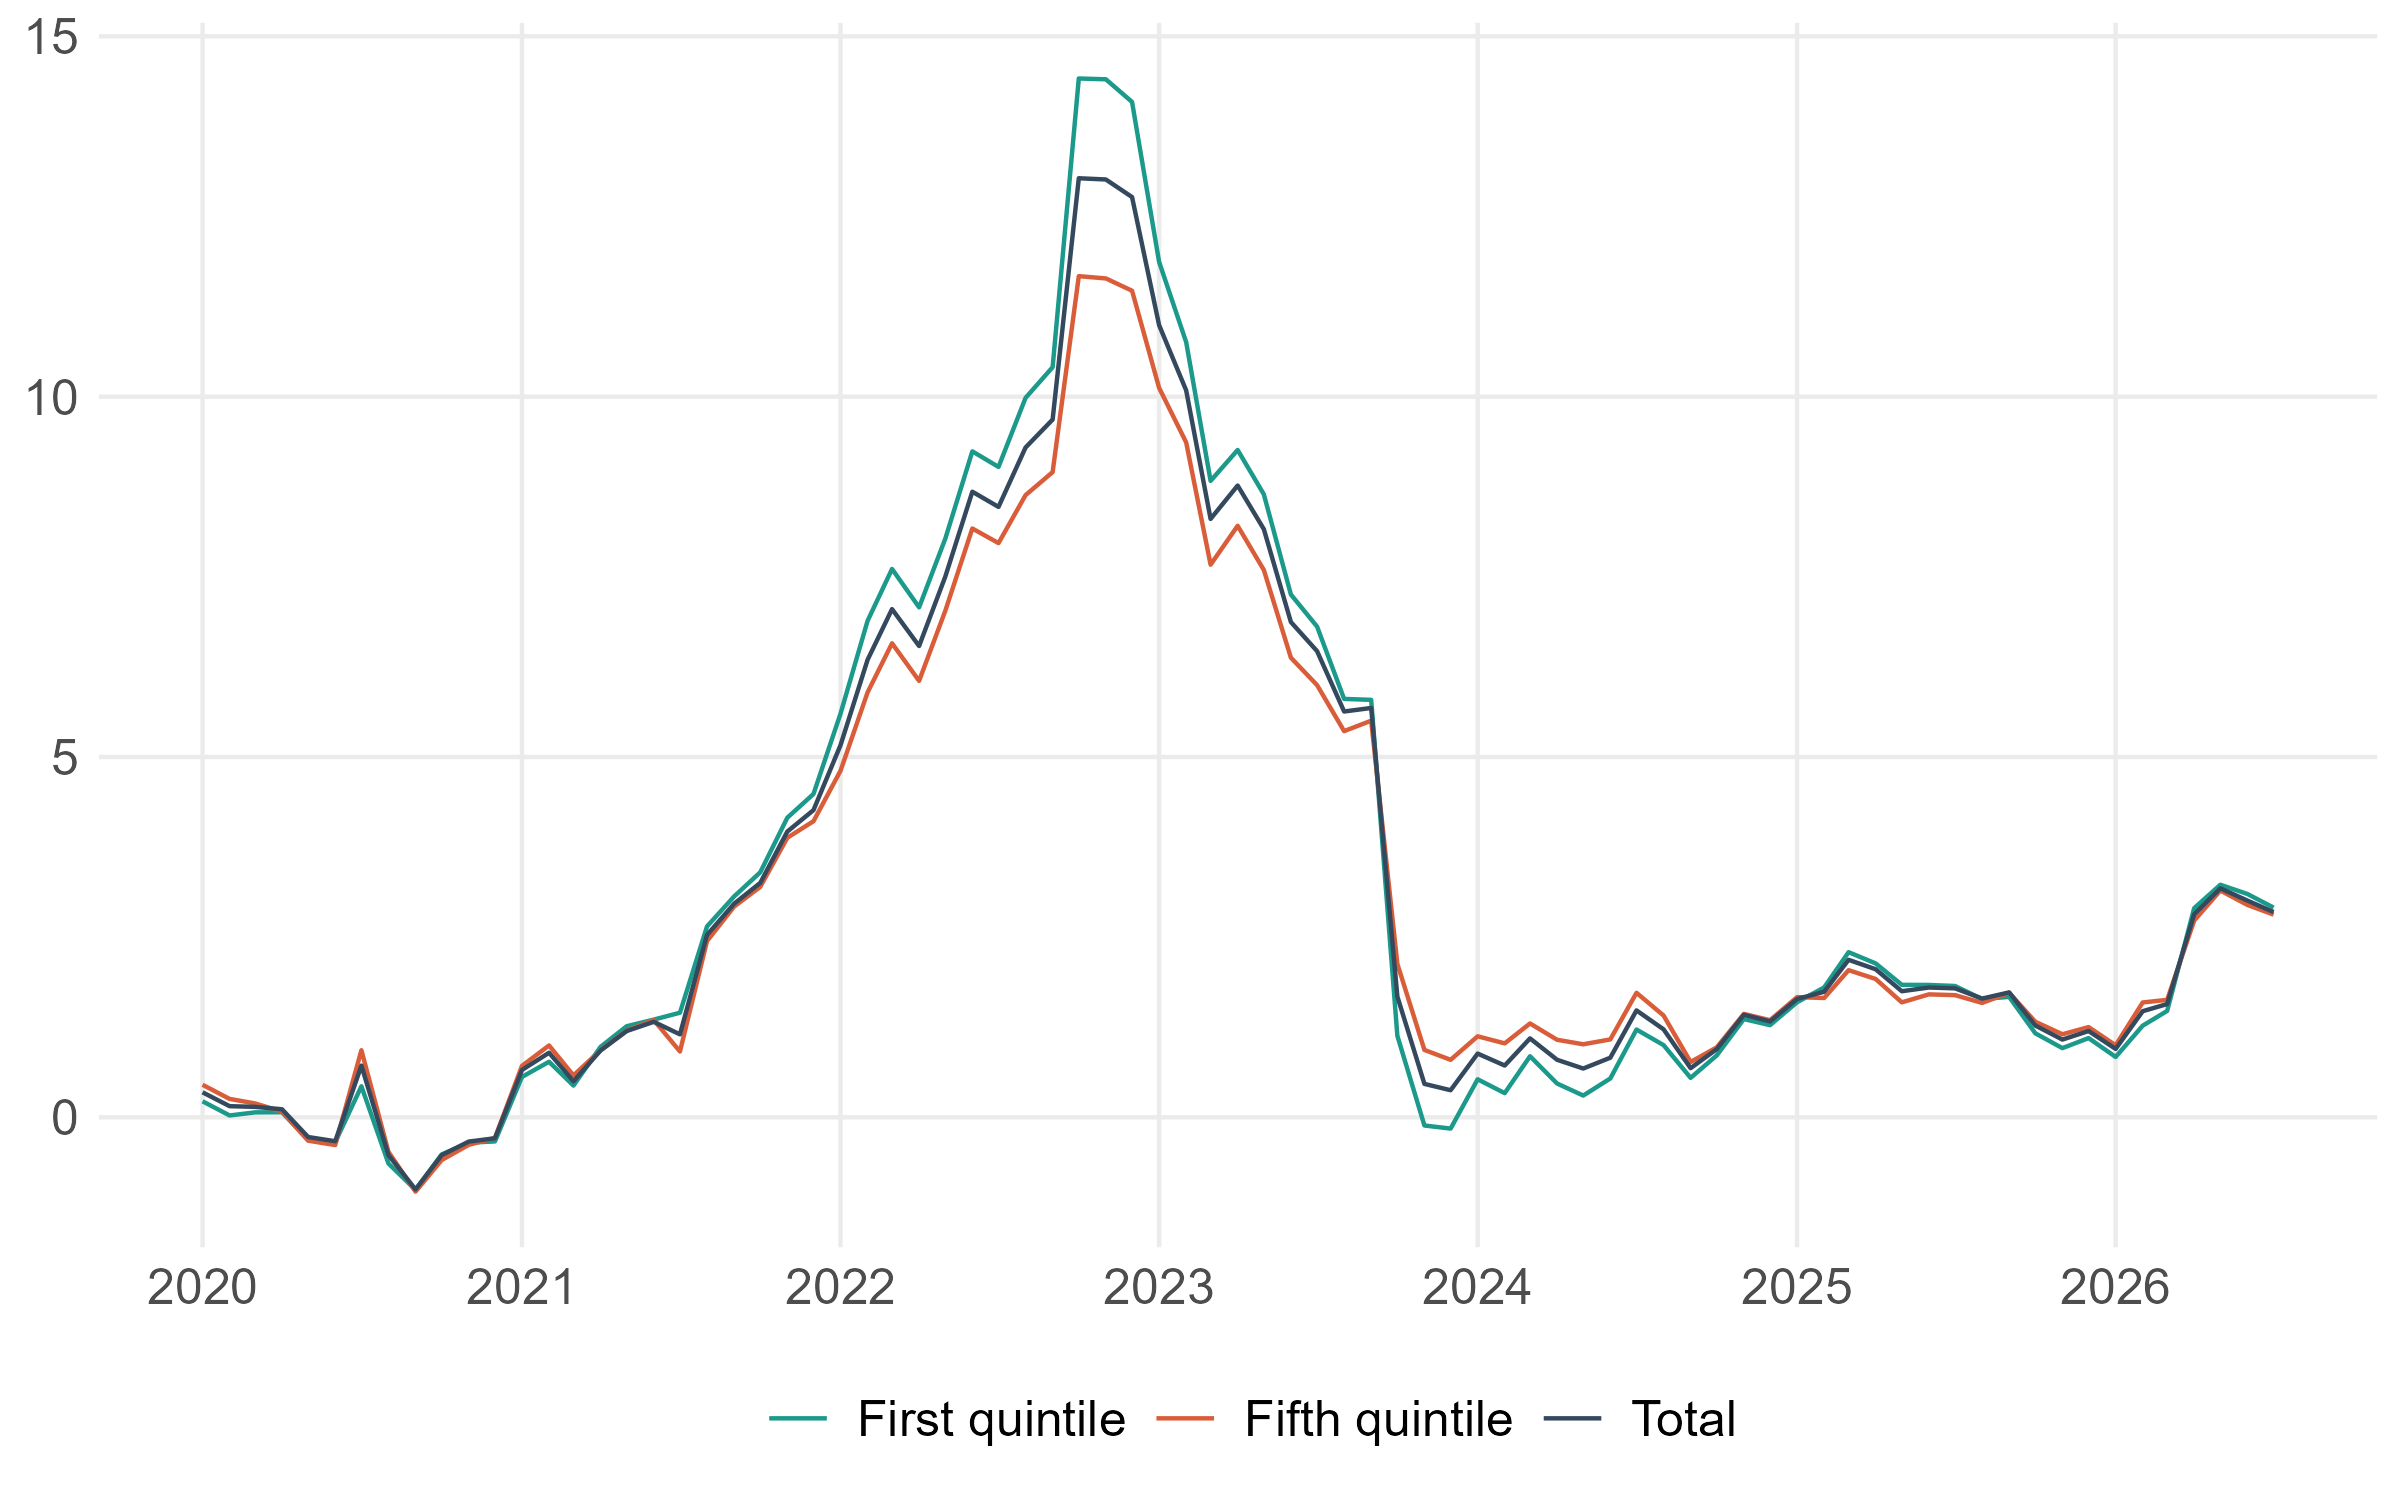
\includegraphics[width=\linewidth,height=0.30\textheight,keepaspectratio]{fig/fig_IT_2019_2026_income_inflation_level2_Q1_Q5.png}
\end{subfigure}
\vspace{6pt}
\begin{subfigure}{0.88\textwidth}
  \centering
  \caption{Age groups}
  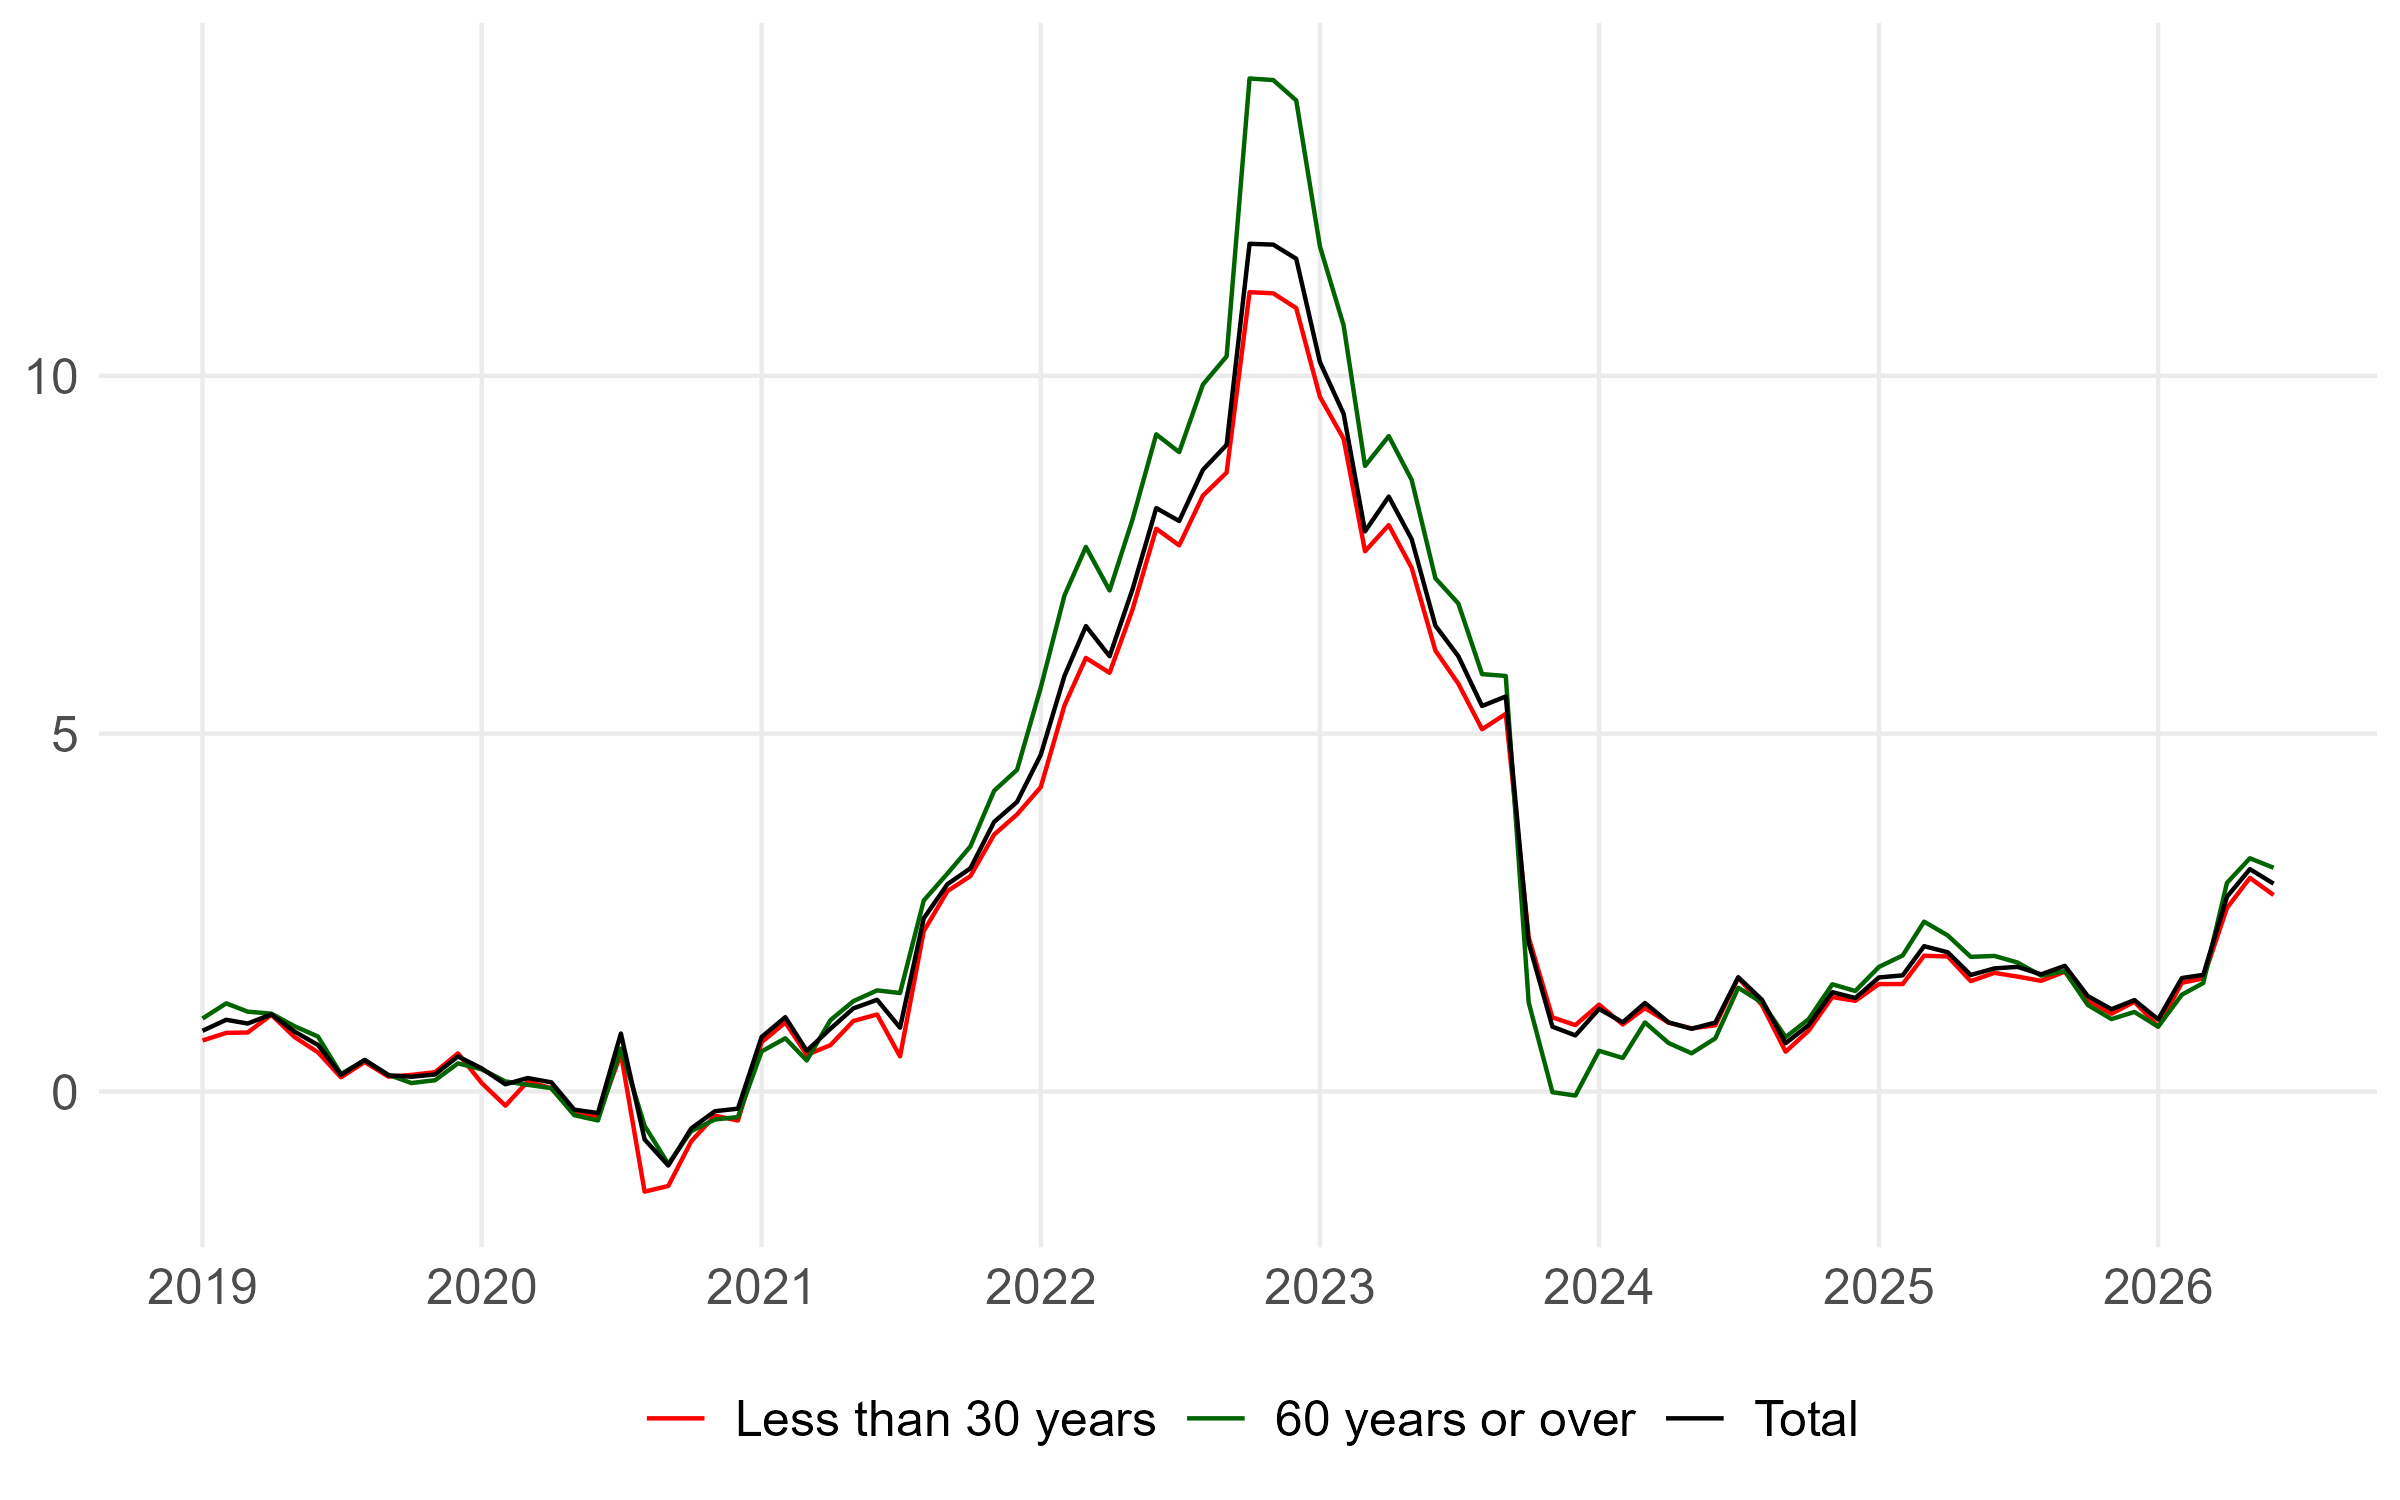
\includegraphics[width=\linewidth,height=0.30\textheight,keepaspectratio]{fig/fig_IT_2019_2026_age_inflation_level2_under30_60plus.png}
\end{subfigure}
\vspace{8pt}
\captionsetup{font=footnotesize, format=hang, singlelinecheck=false, justification=justified}
\caption*{Notes: The figure reports monthly year-on-year inflation rates using RAS weighting for income and age groups.\\
Sources: Eurostat HICP; Italian HBS inputs described in Appendix~\ref{sec:app-italy-hbs}; authors' calculations.}
\end{figure}
\newpage

\begin{figure}[H]
\centering
\caption{Contributions to inflation gaps, Italy, COICOP digit 3 (in pp)}
\label{fig:app-it-level2-contributions}
\begin{subfigure}{0.88\textwidth}
  \centering
  \caption{Income gap: Quintile 1 minus Quintile 5}
  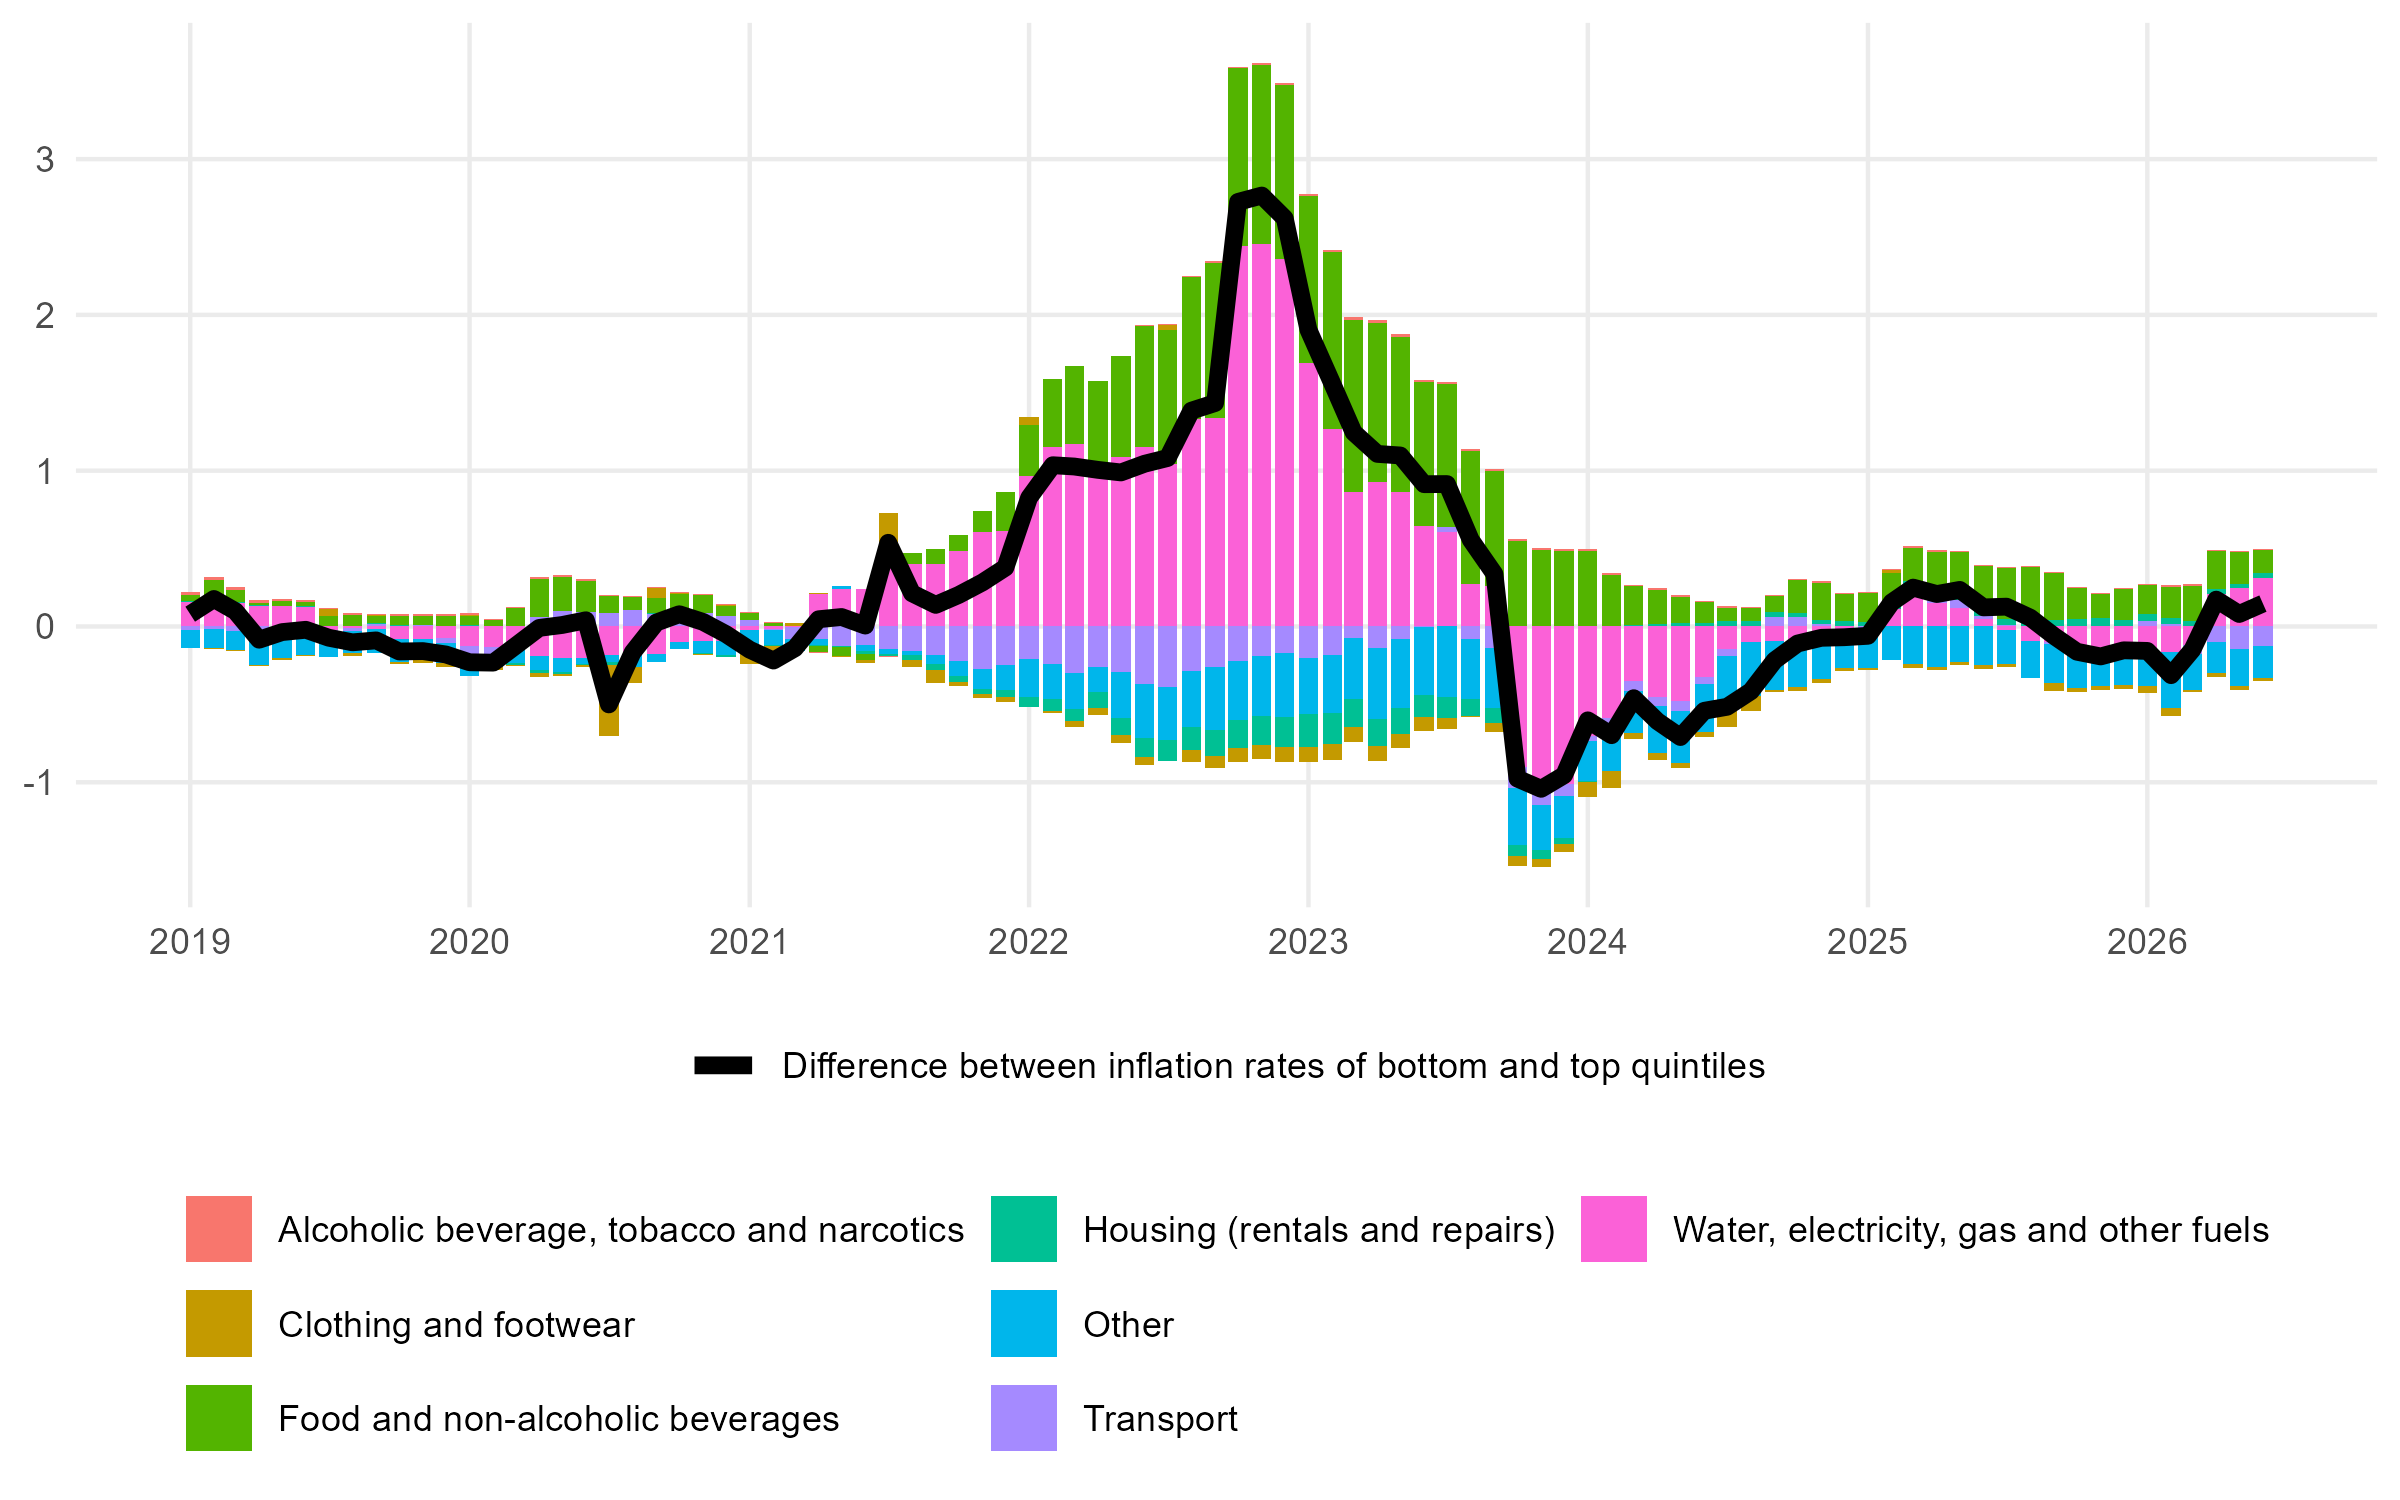
\includegraphics[width=\linewidth,height=0.30\textheight,keepaspectratio]{fig/fig_IT_2019_2026_income_contribution_gap_level2_Q1_Q5.png}
\end{subfigure}
\vspace{6pt}
\begin{subfigure}{0.88\textwidth}
  \centering
  \caption{Age gap: 60 years or over minus under 30}
  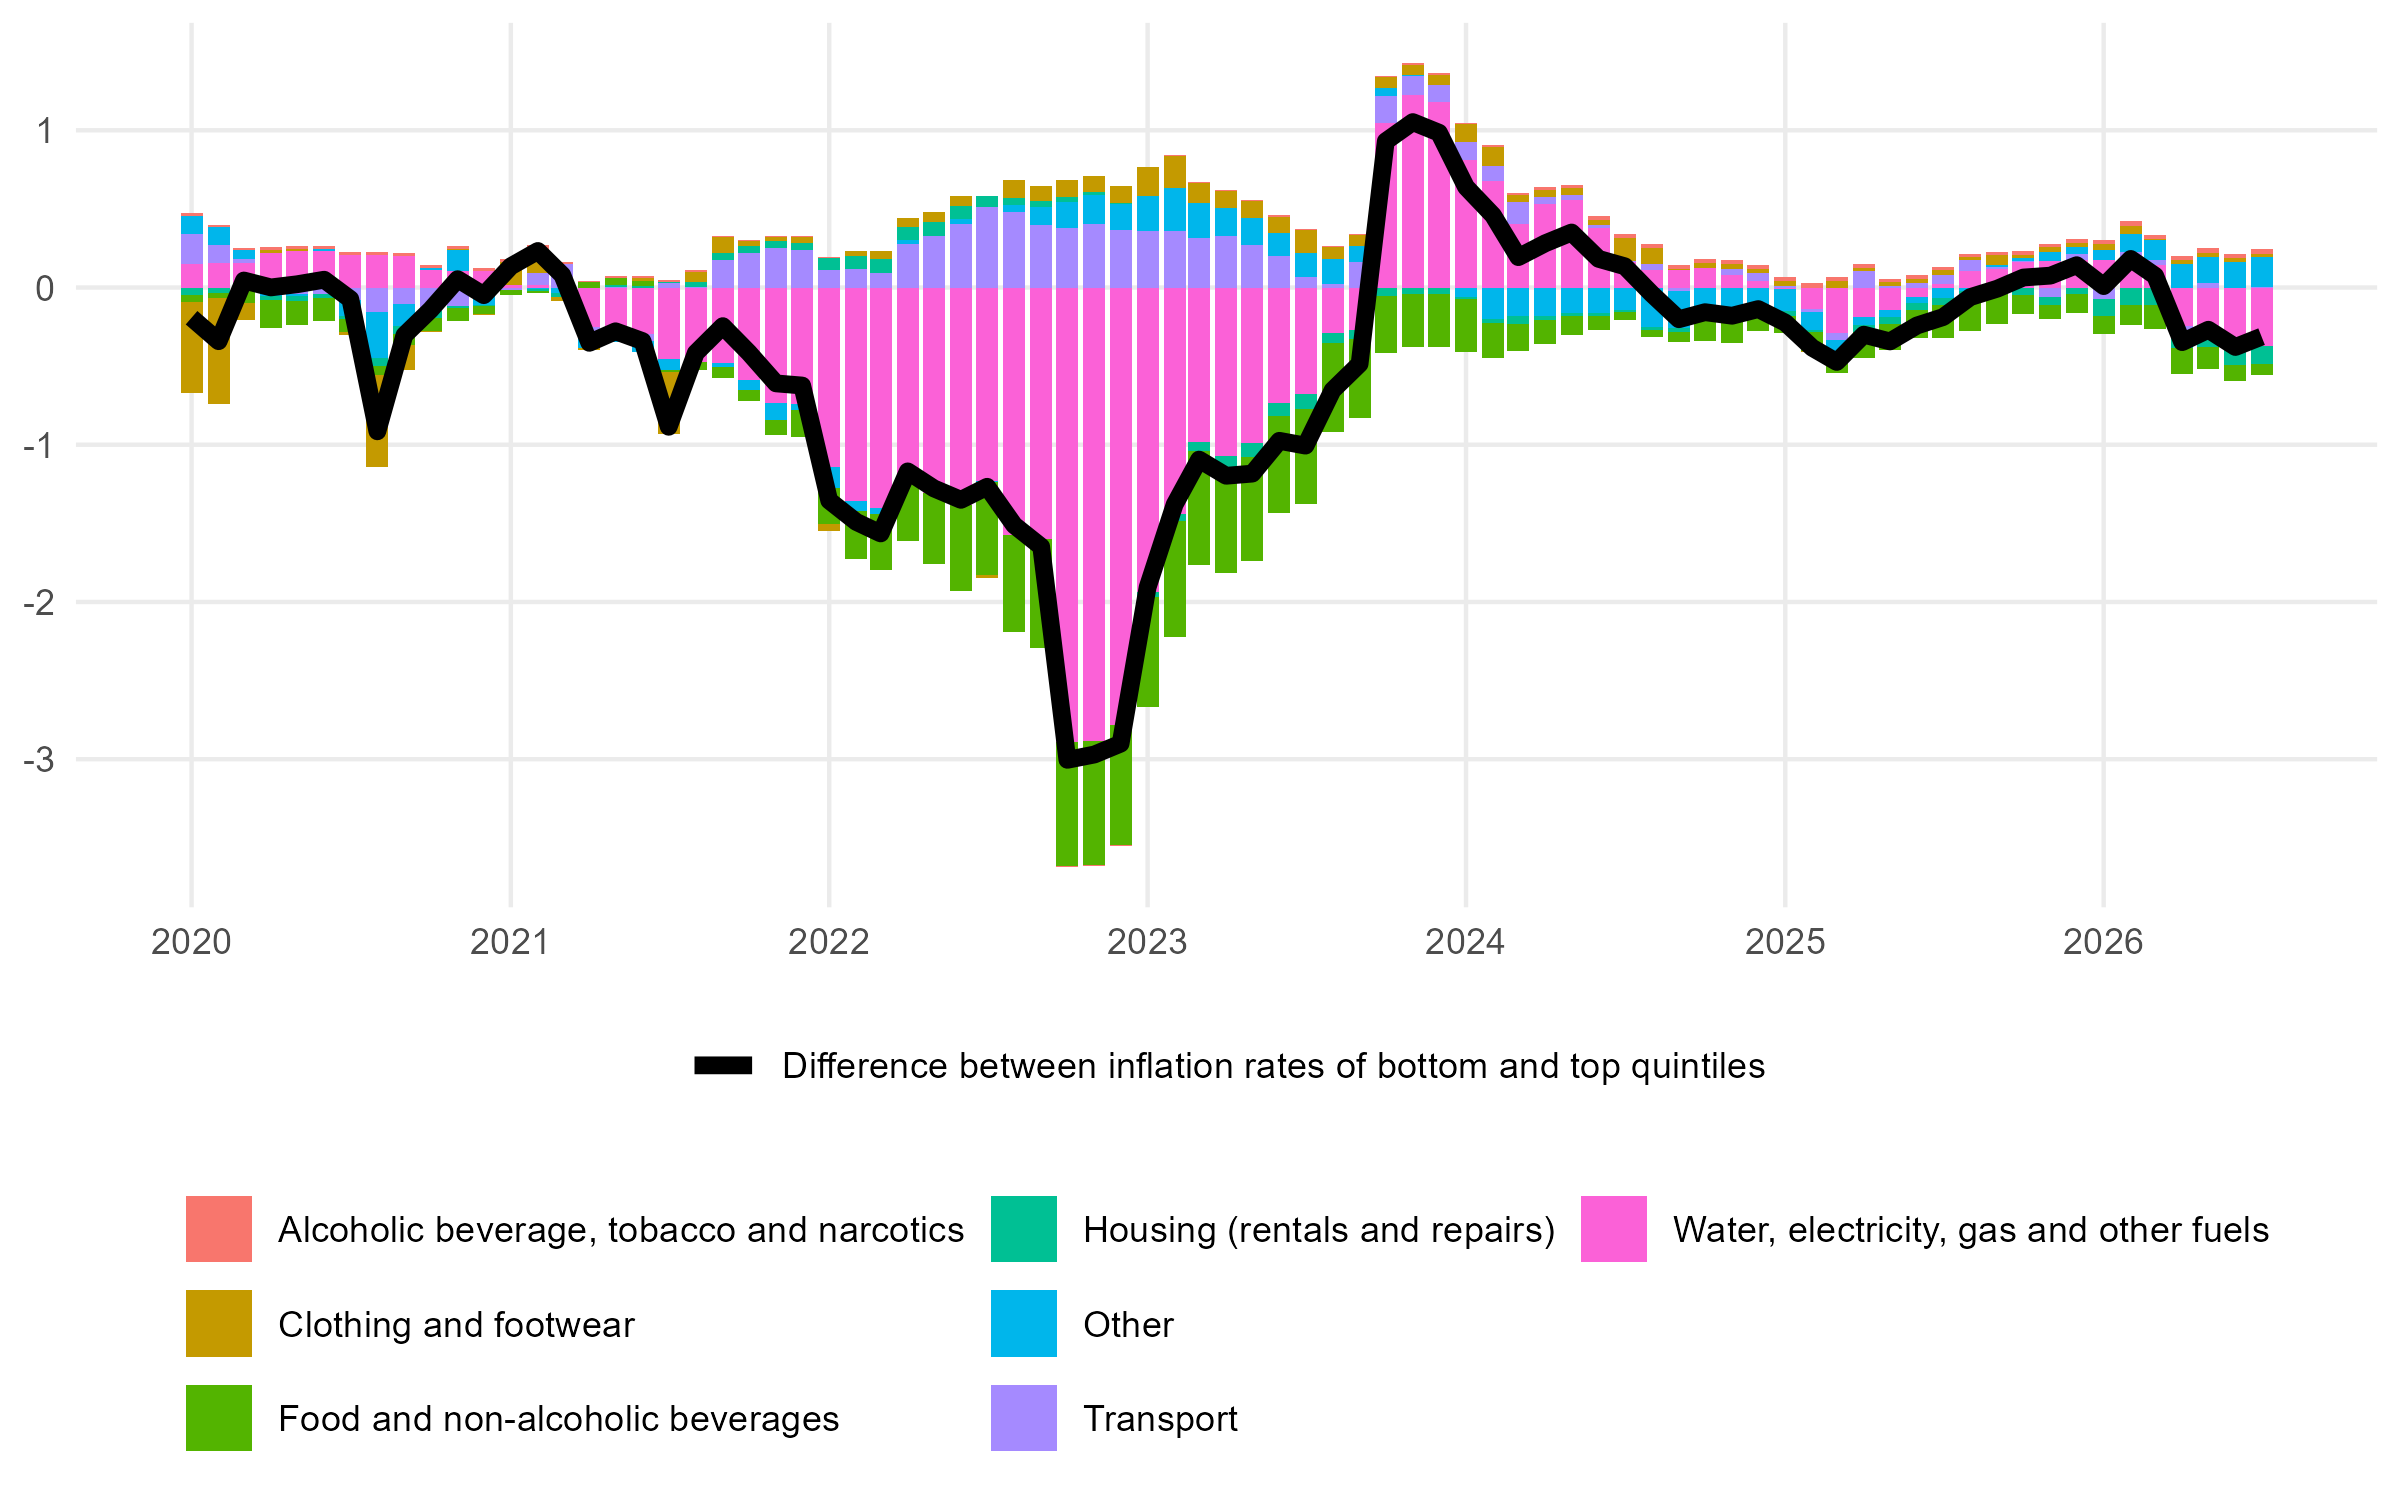
\includegraphics[width=\linewidth,height=0.30\textheight,keepaspectratio]{fig/fig_IT_2019_2026_age_contribution_gap_level2_60plus_under30.png}
\end{subfigure}
\vspace{8pt}
\captionsetup{font=footnotesize, format=hang, singlelinecheck=false, justification=justified}
\caption*{Notes: Bars decompose the monthly inflation gap into broad consumption components; the black line reports the total gap. Positive values indicate higher inflation for the first group named in each panel.\\
Sources: Eurostat HICP; Italian HBS inputs described in Appendix~\ref{sec:app-italy-hbs}; authors' calculations.}
\end{figure}
\newpage

\section{RAS Weighting}
\label{sec:app-weight-normalization}

We use the RAS (Row and Column Adjustment Scaling) algorithm. RAS is a bi-proportional matrix
scaling method that alternately rescales rows and columns until the required marginal totals are
matched \citep{bacharach1965estimating}. In our setting, we combine official HICP item weights with
the relative HBS expenditure profile of each household group.

We retain imputed rents in the HBS expenditure profiles even though they are not included in the
official HICP. Dropping them before normalizing each group's expenditures would implicitly treat
owner-occupiers as consuming no housing services and would mechanically redistribute the omitted
housing share across all remaining items. This is not a neutral rescaling: homeownership, and hence
the imputed-rent share, varies systematically across income, age, and residence-area groups. The
normalization would therefore inflate the non-housing weights most strongly for groups with high
homeownership rates, potentially attributing differences in measured inflation to their consumption
patterns when they instead arise from unequal omitted housing shares. \citet{geerolf2023inflation}
shows that this bias can be quantitatively important: because imputed rents are relatively more
important for richer, older, and rural households, excluding them can overstate their inflation and
can even reverse comparisons between household groups. We therefore preserve imputed rents in the
group-level HBS profiles used by the calibration. Their inclusion should be understood as a safeguard
against group-specific normalization bias, rather than as a claim that imputed rents belong to the
official HICP coverage.

Table~\ref{tab:rent-mapping-robustness} quantifies this sensitivity across countries. The baseline
combines HBS actual and imputed rents (041+042) before mapping them to HICP actual rents (041). The
first alternative retains only HBS actual rents, while the second removes rents from both the HBS
profiles and the HICP basket and renormalizes all remaining items.

%%%%%%%%%%%%%%%%%%%%%%%%%%%%%%%%%%%%%%%%%%%%%%%%%%%%%%%%%%%%%%
\begin{table}[H]
\scriptsize
\setlength{\tabcolsep}{2.5pt}
\renewcommand{\arraystretch}{1.05}

\caption{\label{tab:rent-mapping-robustness}Robustness of income-group inflation to the treatment of rents, June 2021--June 2023}
\centering
\begin{tabular}[t]{lllllll}
\toprule
 & \multicolumn{2}{c}{HBS 041+042 $\to$ HICP 041} & \multicolumn{2}{c}{HBS 041 $\to$ HICP 041} & \multicolumn{2}{c}{Excluding rents}\\
\cmidrule(lr){2-3} \cmidrule(lr){4-5} \cmidrule(lr){6-7}
Country & Cumulative inflation & Inflation gap & Cumulative inflation & Inflation gap & Cumulative inflation & Inflation gap\\
\midrule
Austria & 17.2 & 0.4 & 17.1 & -0.2 & 18.3 & 0.8\\
Belgium & 12.3 & -1.1 & 11.3 & -1.6 & 11.9 & -1.1\\
Croatia & 21.4 & -0.6 & 21.1 & -0.6 & 21.3 & -0.6\\
Cyprus & 12.0 & 0.7 & 12.6 & 0.6 & 12.9 & 0.8\\
Estonia & 33.0 & 7.5 & 38.4 & 7.1 & 38.8 & 7.4\\
\addlinespace
Finland & 12.5 & -1.2 & 10.0 & -3.3 & 12.8 & -0.7\\
France & 12.2 & 0.2 & 11.2 & -1.3 & 13.2 & 0.4\\
Germany & 15.6 & 1.3 & 14.7 & -1.2 & 18.4 & 2.0\\
Greece & 14.7 & 0.6 & 14.6 & -0.0 & 15.6 & 0.8\\
Ireland & 14.9 & 3.8 & 17.5 & 4.4 & 16.9 & 4.0\\
\addlinespace
Italy & 15.8 & 2.1 & 17.2 & 2.1 & 17.7 & 2.3\\
Latvia & 28.9 & 9.5 & 36.1 & 9.6 & 36.6 & 9.9\\
Lithuania & 30.4 & 4.6 & 33.5 & 4.5 & 33.6 & 4.7\\
Luxembourg & 11.4 & -0.2 & 10.0 & -1.5 & 11.4 & -0.2\\
Malta & 12.7 & 1.6 & 13.8 & 1.6 & 13.0 & 0.9\\
\addlinespace
Netherlands & 16.9 & 1.2 & 15.5 & -1.7 & 19.8 & 2.4\\
Portugal & 14.2 & -2.3 & 12.5 & -3.0 & 13.4 & -2.3\\
Slovakia & 25.4 & 2.7 & 26.1 & 2.0 & 27.3 & 3.0\\
Slovenia & 18.1 & 2.4 & 20.1 & 2.7 & 19.7 & 2.2\\
Spain & 11.8 & 0.1 & 11.3 & -0.6 & 12.2 & 0.2\\
\addlinespace
\midrule
\textbf{Euro area} & \textbf{14.7} & \textbf{0.9} & \textbf{14.2} & \textbf{-0.5} & \textbf{16.3} & \textbf{1.3}\\
\bottomrule
\end{tabular}
\vspace{-0.4em}
\begin{flushleft}
\footnotesize{Notes. Cumulative inflation refers to Q1; the gap is Q1 minus Q5. The baseline combines actual and imputed rent expenditure; alternatives use actual rent only or exclude rent. Entries are percentage points. Sources: Eurostat, authors' calculations.}
\end{flushleft}
\end{table}

%%%%%%%%%%%%%%%%%%%%%%%%%%%%%%%%%%%%%%%%%%%%%%%%%%%%%%%%%%%%%%

We distinguish three objects: the HICP product shares, the aggregate product-by-group expenditure
mass calibrated by RAS, and the resulting within-group baskets. First, let $s_{g,y}$ denote the
share of group $g$ in total consumption expenditure used for HICP weight year $y$:
\begin{equation}
s_{g,y}
=
\frac{E^{\mathrm{HBS}}_{g,y'}}{E^{\mathrm{HBS}}_{\mathrm{all},y'}},
\qquad
\sum_g s_{g,y}=1,
\end{equation}
where $y'$ is the HBS wave matched to HICP weight year $y$. In the implementation, $s_{g,y}$ is
selected from the group consumption-share table using the most recent HBS wave available at or
before $y$; if no prior wave is available, the earliest available wave is used. These targets are
expenditure shares, not population shares. For Italy, the income targets use the Istat-based HBS
inputs described in Appendix~\ref{sec:app-italy-hbs}.

Let $\mathcal{J}_y$ be the set of matched COICOP categories available in the HICP weighting
structure in year $y$. Let $E^{\mathrm{HBS}}_{j,g,y'}$ denote expenditure on item $j$ by group $g$ in the
matched HBS wave $y'$, and let $E^{\mathrm{HBS}}_{j,\mathrm{all},y'}$ denote expenditure on that item by all
households. Consistently with the implementation, the HBS correction factor used in the RAS seed is
the share of aggregate expenditure on item $j$ accounted for by group $g$:
\begin{equation}
c^{\mathrm{HBS}}_{j,g,y'}
=
\frac{E^{\mathrm{HBS}}_{j,g,y'}}{E^{\mathrm{HBS}}_{j,\mathrm{all},y'}}.
\end{equation}
Thus $c^{\mathrm{HBS}}_{j,g,y'}$ records how expenditure on item $j$ is distributed across household groups.
To avoid mixing index-weight units with expenditure shares, define the HICP weight normalized over
the matched product set as
\begin{equation}
\bar{\omega}^{\mathrm{HICP}}_{j,y}
=
\frac{\omega^{\mathrm{HICP}}_{j,y}}
{\sum_{k \in \mathcal{J}_y}\omega^{\mathrm{HICP}}_{k,y}},
\qquad
\sum_{j \in \mathcal{J}_y}\bar{\omega}^{\mathrm{HICP}}_{j,y}=1.
\end{equation}
The initial product-by-group mass is then
\begin{equation}
Z_{j,g,y}
=
\max\left\{
s_{g,y}\bar{\omega}^{\mathrm{HICP}}_{j,y}c^{\mathrm{HBS}}_{j,g,y'},\epsilon
\right\},
\qquad
\epsilon=10^{-12}.
\end{equation}
The small positive floor is a numerical safeguard to keep the RAS problem strictly non-negative
after HICP-HBS matching. RAS transforms this seed into a joint expenditure-share matrix
$M_{j,g,y}$. Its group margins equal the groups' expenditure shares, while its product margins equal
the normalized HICP shares:
\begin{equation}
\sum_{j \in \mathcal{J}_y} M_{j,g,y}
=
s_{g,y}
\quad \text{for all } g,
\qquad
\sum_g M_{j,g,y}
=
\bar{\omega}^{\mathrm{HICP}}_{j,y}
\quad \text{for all } j.
\end{equation}
Both sets of margins sum to one, so the constraints are mutually compatible.

The RAS algorithm starts from $M^{(0)}_{j,g,y}=Z_{j,g,y}$ and repeats two scaling steps. At
iteration $t$, the group-margin adjustment is
\begin{equation}
\widetilde{M}^{(t)}_{j,g,y}
=
M^{(t-1)}_{j,g,y}
\times
\frac{
s_{g,y}
}{
\sum_{\ell \in \mathcal{J}_y} M^{(t-1)}_{\ell,g,y}
},
\end{equation}
and the product-margin adjustment is
\begin{equation}
M^{(t)}_{j,g,y}
=
\widetilde{M}^{(t)}_{j,g,y}
\times
\frac{
\bar{\omega}^{\mathrm{HICP}}_{j,y}
}{
\sum_h \widetilde{M}^{(t)}_{j,h,y}
}.
\end{equation}
We iterate these two steps by weight year until the maximum absolute row or column marginal error is
below $10^{-10}$, with a maximum of 1,000 iterations.

The calibrated matrix $M$ is a joint expenditure distribution. The group-specific HICP basket is
the corresponding conditional product distribution within group $g$:
\begin{equation}
\omega_{j,g,y}
=
\frac{M_{j,g,y}}{s_{g,y}}
=
\frac{M_{j,g,y}}{\sum_{k \in \mathcal{J}_y}M_{k,g,y}}.
\end{equation}
The equality of the two denominators follows directly from the group-margin constraint. It implies
that each group basket sums to one. Moreover, the expenditure-share-weighted average of the group
baskets reproduces the normalized HICP product weights:
\begin{equation}
\sum_{j \in \mathcal{J}_y}\omega_{j,g,y}=1,
\qquad
\sum_g s_{g,y}\omega_{j,g,y}
=
\bar{\omega}^{\mathrm{HICP}}_{j,y}.
\end{equation}

The package implements the same system on a percentage scale. Internally, the calibrated mass is
$M^{\mathrm{pct}}_{j,g,y}=100M_{j,g,y}$, so its margins are $100s_{g,y}$ and
$100\bar{\omega}^{\mathrm{HICP}}_{j,y}$. The package returns
these percentage weights in the R variable \texttt{weighted\_consumption}. Denoting this variable
by $w^{\mathrm{code}}_{j,g,y}$, we have
\begin{equation}
w^{\mathrm{code}}_{j,g,y}
=
\frac{M^{\mathrm{pct}}_{j,g,y}}{s_{g,y}}
=
100\omega_{j,g,y},
\end{equation}
and sums to 100 within every household group. Thus division by $s_{g,y}$ in the code is the
percentage-scale counterpart of dividing $M_{j,g,y}$ by its group-row sum in the normalized
mathematical representation.

This preserves the relative information contained in the HBS expenditure profiles while making the
aggregate of the household-group baskets consistent with the published HICP weighting structure, up
to residual differences induced by product coverage and COICOP matching.

Table~\ref{tab:de-normalization-validation} compares the two weights for Germany at COICOP digit 3
over the period beginning in 2019. The RAS
calibration tracks the published German HICP more closely than the relative-expenditure weighting, whose implicit aggregate weights are equal across groups.%$\omega_{j,y)}*\c_{j,g,y'}$

\begin{table}[H]
\centering
\caption{\label{tab:de-normalization-validation}Germany HICP validation by weighting scheme (differences in pp)}
\small
\begin{tabular}{lrrrrr}
\toprule
Method & Obs. & Mean diff. & Mean abs. diff. & RMSE & Max abs. diff. \\
\midrule
RAS & 88 & -0.059 & 0.093 & 0.118 & 0.259 \\
Relative expenditure & 88 & -0.070 & 0.143 & 0.166 & 0.449 \\
\bottomrule
\end{tabular}
\begin{minipage}{0.86\textwidth}
\footnotesize
\emph{Notes:} Validation statistics compare the recalculated average of German
income-quintile inflation rates with the published all-items HICP inflation
rate. The sample is monthly, from January 2019 to April 2026. All differences
are recalculated minus published inflation and are reported in percentage
points.
\end{minipage}
\end{table}




\clearpage
\begingroup
\setlength{\textfloatsep}{4pt plus 1pt minus 1pt}
\setlength{\floatsep}{4pt plus 1pt minus 1pt}
\setlength{\intextsep}{4pt plus 1pt minus 1pt}
\captionsetup{font=scriptsize,hypcap=false}

\section{Validation Tests}
\label{sec:app-validation-tests}
\enlargethispage{2\baselineskip}

This appendix reports three validation checks for the recalculated French inflation series:
agreement with published HICP, aggregation of quintile inflation rates, and comparison with official
INSEE decile inflation.

\vspace{-0.5em}
\subsection{Internal Consistency}

Figure~\ref{fig:fr-validation-rate} compares COICOP digit-3 RAS recalculated French inflation with
published all-items HICP. Figure~\ref{fig:fr-validation-level} compares the total inflation rate
with the expenditure-weighted average of income-quintile inflation rates.

%%%%%%%%%%%%%%%%%%%%%%%%%%%%%%%%%%%%%%%%%%%%%%%%%%%%%%%%%%%%%%
\begin{center}
\centering
\captionof{figure}{Internal consistency: France total inflation and published HICP, COICOP digit 3 RAS (in \%)}\label{fig:fr-validation-rate}
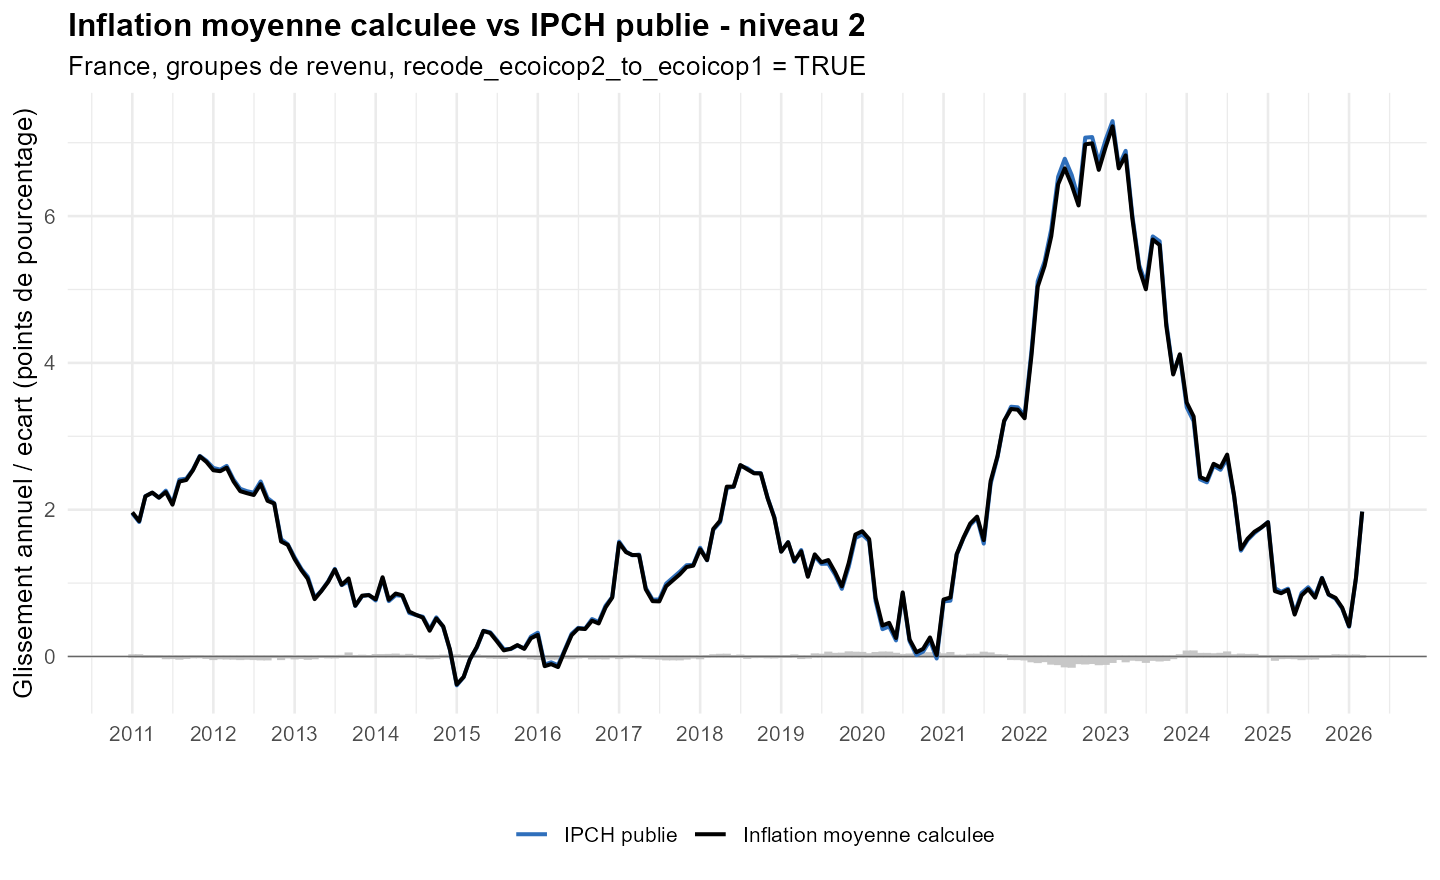
\includegraphics[width=0.95\textwidth,height=0.22\textheight,keepaspectratio]{fig/fig_FR_2010_2026_hicp_inflation_validation_level2_recode_mean_vs_published.png}
\vspace{-2pt}
\captionsetup{font=scriptsize, format=hang, singlelinecheck=false, justification=justified}
\caption*{Notes: Blue line: published all-items HICP. Black line: recalculation from 2019 onward. Grey bars: recalculation minus published HICP, in points.\\
Sources: INSEE, Eurostat, authors' calculations.}
\end{center}

%%%%%%%%%%%%%%%%%%%%%%%%%%%%%%%%%%%%%%%%%%%%%%%%%%%%%%%%%%%%%%
\begin{center}
\centering
\captionof{figure}{Internal consistency: France total inflation and weighted average of quintiles, COICOP digit 3 RAS (in \%)}\label{fig:fr-validation-level}
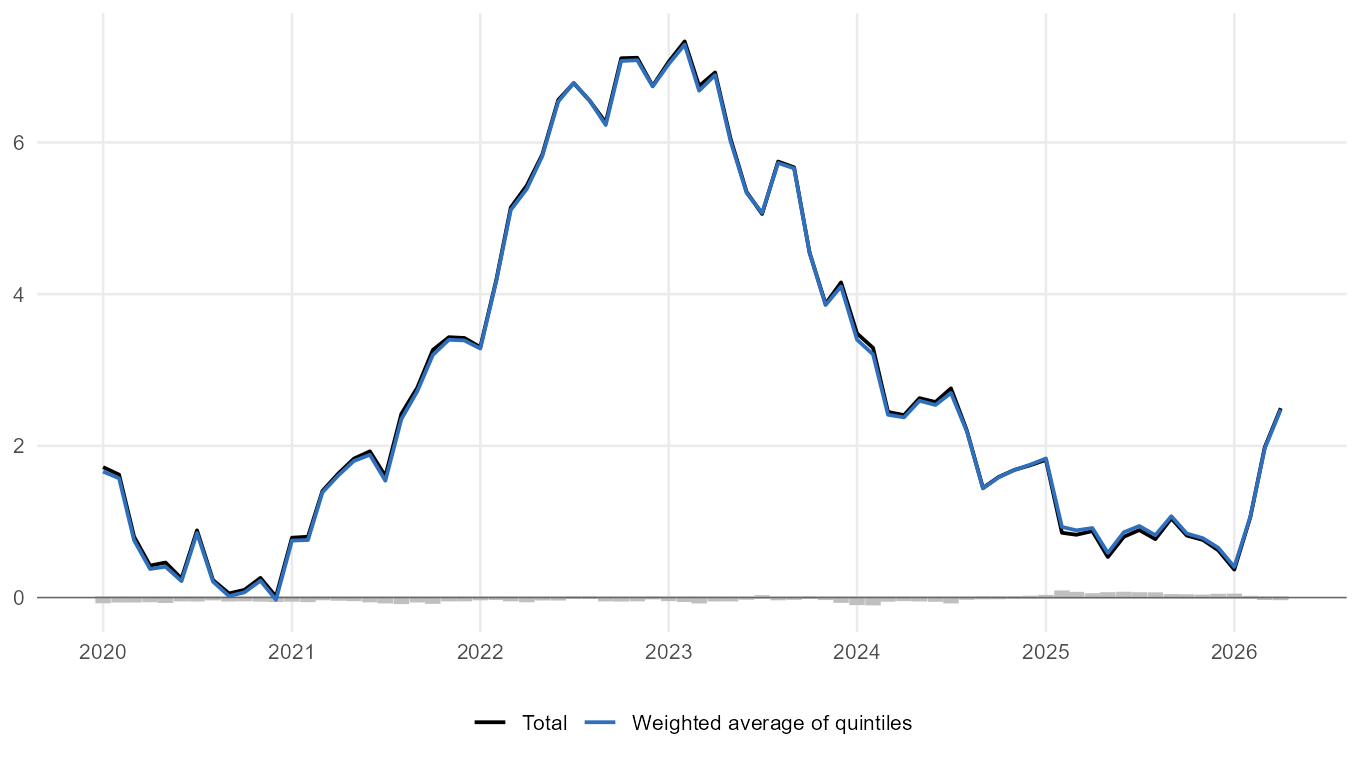
\includegraphics[width=0.95\textwidth,height=0.22\textheight,keepaspectratio]{fig/fig_FR_2010_2026_hicp_validation_level_mean_vs_published.png}
\vspace{-2pt}
\captionsetup{font=scriptsize, format=hang, singlelinecheck=false, justification=justified}
\caption*{Notes: Recalculated total inflation and the weighted average of recalculated income-quintile inflation rates. Grey bars: weighted average minus total, in points.\\
Sources: INSEE, Eurostat, authors' calculations.}
\end{center}
%%%%%%%%%%%%%%%%%%%%%%%%%%%%%%%%%%%%%%%%%%%%%%%%%%%%%%%%%%%%%%
\endgroup

\clearpage
\subsection{External Consistency}

Figure~\ref{fig:fr-decile-published-recalculated} compares the annualized inflation rates computed
at COICOP digit 4 with the official INSEE income decile series.

\begin{figure}[H]
\centering
\caption{External consistency: annual inflation by standard-of-living decile, France (in \%)}
\label{fig:fr-decile-published-recalculated}
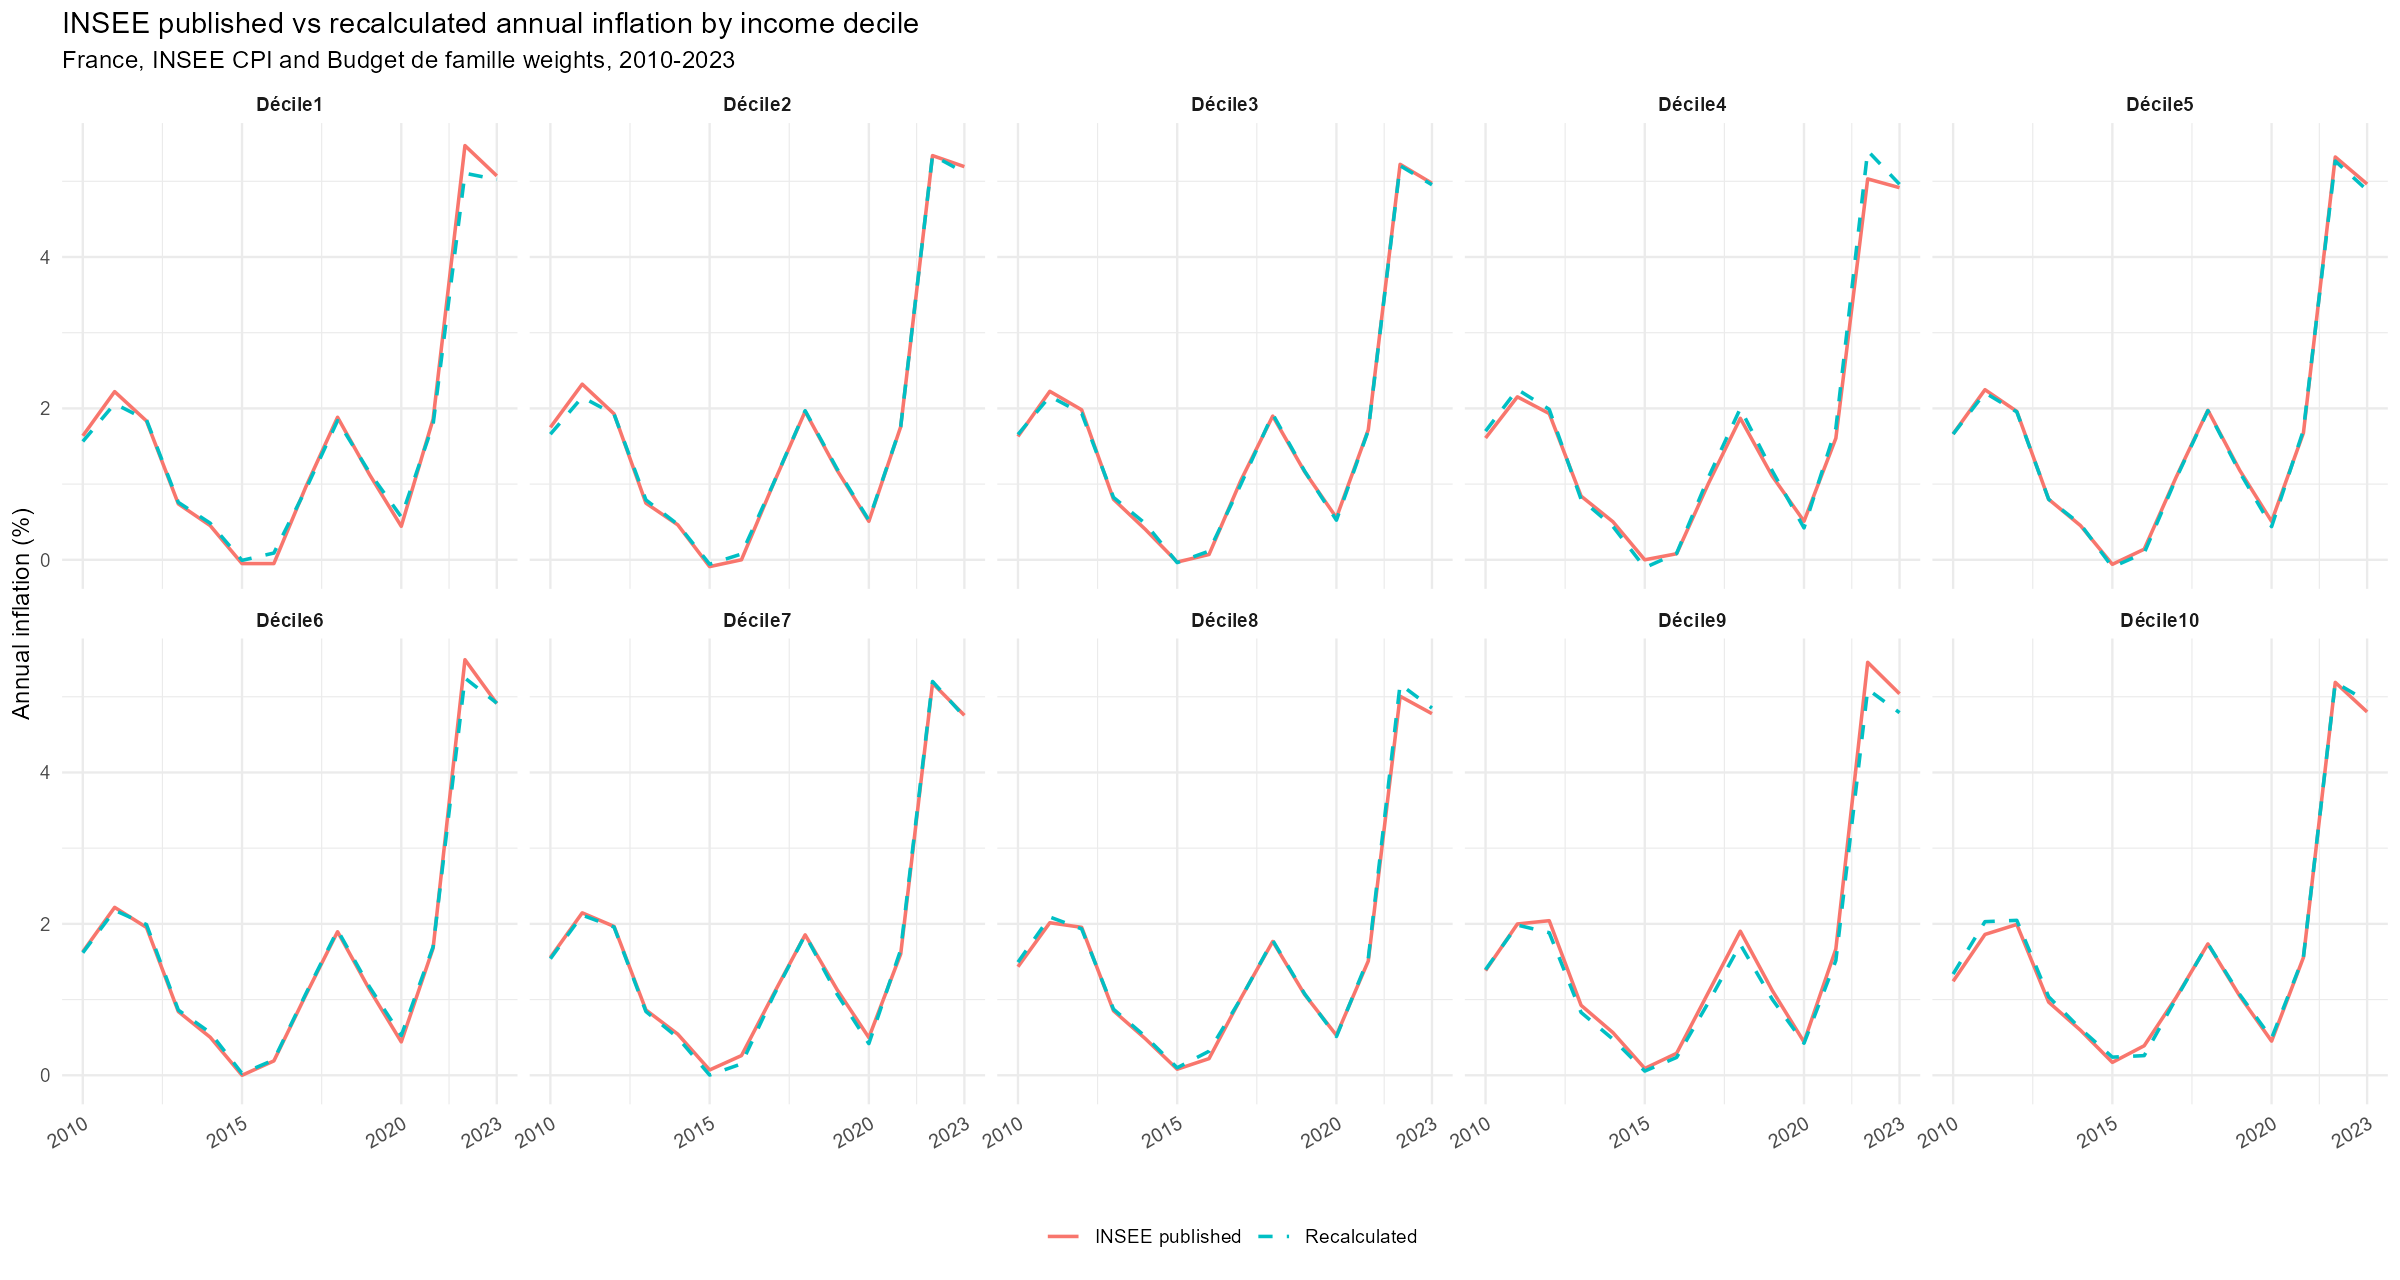
\includegraphics[width=0.98\textwidth,height=0.50\textheight,keepaspectratio]{fig/france-insee-decile-published-vs-recalculated-D1-D10-2010-2023.png}
\captionsetup{font=scriptsize, format=hang, singlelinecheck=false, justification=justified}
\caption*{Notes: Official INSEE annual inflation rates by standard-of-living decile are compared with the recalculated series.\\
Sources: INSEE, Eurostat, authors' calculations.}
\end{figure}

\end{document}
